\documentclass[a4paper,11pt,twoside]{book}
% Template Latex pour les thèses à Paris Sciences et Lettres (PSL university)

% Issu de template de Pierre Guillou https://pierre.guillou.net/psl-cover/2018/ (Version 1.2 (20 juillet 2019))
% couvertures accessibles sur le site du college doctoral de PSL : https://collegedoctoral.psl.eu/doctorat-psl/espace-ressources/

% Proposé par Arthur Chavignon, février 2022

% Encodage des caractères et langue du document
\usepackage{setspace}
\usepackage[T1]{fontenc}
\usepackage[utf8]{inputenc}
\usepackage{lmodern}
%\usepackage[english,french]{babel}
\usepackage[english]{babel}
\usepackage{textgreek}

\setcounter{tocdepth}{3} % Pour que les subsubsections n'apparaissent pas dans la TOC
\setcounter{secnumdepth}{3} % Pour que les subsubsections ne soient pas numérotées
%\usepackage{fixltx2e}

%%%%%%%%%% Gestions des marges %%%%%%%%%%
\usepackage{geometry} % Si on a besoin d'une configuration plus précise des marges
\geometry{a4paper,                % format de papier
% Définition des marges :
  left= 3cm,right = 2cm,  % marge intérieure extérieure à la page
  top = 3cm,bottom = 3cm,
% En-tête et pied de page :
  headheight=6mm,         % espace réservé à l'en-tête dans la marge top
  %headsep=3mm,            % espace entre le corps et l'en-tête
  %footskip=9mm            % espace entre le corps et le pied de page
  marginparwidth = 16mm
}

\raggedbottom
\reversemarginpar
% \usepackage{showframe} % pour afficher les traits des marges

%%%%%%%%%%%%%%%%%%%%%%%%%%%%%%%%%%%%%%%%%%%%%%%%%%%%%%%%%%%%%%%%%%%%
%%%%%%%%%%% Gestion maths %%%%%%%%%%
\usepackage{amsmath,amssymb,amsfonts,amsthm}
\usepackage{mathtools} % version modifiée de amsmath, ajoute des symboles, etc.
\usepackage{mathrsfs}% pour rajouter un format de lettres façon calligraphie en math mode.
\DeclareMathOperator{\sinc}{sinc}
\DeclareMathOperator{\e}{e}

%\usepackage[locale = FR]{siunitx} % Pour gérer les unités
%\sisetup{inter-unit-product=\ensuremath{{}\cdot{}}} % pour mettre des points médians entre les unités quand il y en a plusieurs
%\sisetup{separate-uncertainty=true,multi-part-units=single} % pour faire des incertitudes en écrivant \SI{valeur(incertitude)}{unité}
%\DeclareSIUnit\vitesse{\meter\per\second}
%\usepackage{eurosym}
%\DeclareSIUnit{\octet}{o}

%%%%%%%%%%%%%%%%%%%%%%%%%%%%%%%%%%%%%%%%%%%%%%%%%%%%%%%%%%%%%%%%%%%%
%%%%%%%%%%%  Graphics / Table / List %%%%%%%%%%%
\usepackage{graphicx,array,tikz,multirow}
\usepackage{caption,subcaption} % permet de faire des subfigures (remplace le package subfig)
\usepackage{svg,float}
\usepackage{booktabs,paralist}
\newcolumntype{x}[1]{>{\centering\arraybackslash\hspace{0pt}}p{#1}}
\usepackage[section]{placeins}
\usepackage{hanging}

%%%%%%%%%%%%%%%%%%%%%%%%%%%%%%%%%%%%%%%%%%%%%%%%%%%%%%%%%%%%%%%%%%%%
%%%%%%%%%%% Header / Foot %%%%%%%%%%%
\usepackage{fancyhdr,emptypage} % garantit que les pages blanches avant les débuts de chapitres soient vraiment blanches (pas d'en-tête ni de pied de page)
\let\cleardoublepage\clearpage

\fancypagestyle{plain}{ %% Page chapitre, toc ...
    \fancyhead{}\fancyfoot[C]{\thepage}
    \renewcommand{\headrulewidth}{0pt}
    \renewcommand{\footrulewidth}{0pt}
}

%%%%%%%%%%% Page normale
\pagestyle{fancy}
    % \renewcommand{\chaptermark}[1]{\markboth{\chaptername \ \thechapter.\ #1}{}} % sert à personnaliser l'affichage de \leftmark (ici : le mot "Chapitre", le numéro, un point, et le titre du chapitre, sans écrire en majuscules)
    % \renewcommand{\chaptermark}[1]{\markleft{\chaptername \ \thechapter.\ #1}{}}
    % \renewcommand{\sectionmark}[1]{\markright{\thesection.\ #1}} % sert à personnaliser l'affichage de \rightmark (ici : le numéro et le titre de la section en cours, sans écrire en majuscules)
    \fancyhf{} % assure que les entête et pieds de page sont vides au départ
    \fancyhead[LE]{\selectfont\nouppercase{\leftmark}}
    \fancyhead[RO]{\selectfont\nouppercase{\rightmark}}
    \fancyfoot[C]{\thepage}
% Explications :
% L = left, R = right, C = center, E = even pages, O = odd pages
%\leftmark : adds name and number of the current top-level structure (for example, Chapter for reports and books classes; Section for articles ) in uppercase letters.
%\rightmark : adds name and number of the current next to top-level structure (Section for reports and books; Subsection for articles) in uppercase letters.

%%%%%%%%%%% Personnaliser les premières pages des chapitres
\usepackage[Lenny]{fncychap}
\ChNameVar{\fontsize{25}{25}\usefont{OT1}{phv}{m}{n}\selectfont}
\ChRuleWidth{0pt}
\ChNumVar{\fontsize{60}{62}\selectfont\textcolor{curcolor}}

\makeatletter
\ChTitleVar{\Huge\rm}
\renewcommand{\DOCH}{%
\setlength{\fboxrule}{\RW} % Let fbox lines be controlled by
\fbox{\CNV\FmN{\@chapapp}\space \CNoV\thechapter}\par\nobreak
\vskip 20\p@}
\renewcommand{\DOTIS}[1]{%
\CTV\bfseries\FmTi{#1}\par\nobreak
\vskip 20\p@}
\makeatother

\renewcommand{\thesection}{\arabic{section}}

% Pour la table des matières
\usepackage[nohints,tight]{minitoc}		% Mini table des matières, en français
\setcounter{minitocdepth}{3} % Mini-toc détaillées (sections/sous-sections)
\setlength{\mtcindent}{-1em} % décalage des minitoc à gauche
\dominitoc

\usepackage[nottoc]{tocbibind} % pour que la bibliographie apparaisse dans la table des matières (avec l'option pour que la table des matières elle-même n'apparaisse pas dans la table des matières).
% \usepackage{tocloft}% pour pouvoir modifier les tailles d'espacement dans la table des matières
\usepackage[titles]{tocloft}

%%%%%%%%%%%%%%%%%%%%%%%%%%%%%%%%%%%%%%%%%%%%%%%%%%%%%%%%%%%%%%%%%%%%
%%%%%%%%%%% Divers %%%%%%%%%%%
\usepackage{textcomp} % rajoute des symboles
\usepackage{xcolor} % pour ajouter de la couleur (si besoin)
\usepackage{epigraph} % pour rajouter des citations en début de chapitre  \epigraph{Citation}}{Auteur}
\usepackage{titling}
\usepackage{lipsum}
\usepackage{csquotes} % added 07/09/21

\usepackage{xspace}
\usepackage{afterpage}
\renewcommand{\baselinestretch}{1.2} % interligne

\usepackage[textsize=footnotesize]{todonotes}




%%%%%%%%%%%%%%%%%%%%%%%%%%%%%%%%%%%%%%%%%%%%%%%%%%%%%%%%%%%%%%%%%%%%
%%%%%%%%%%% Links ref  %%%%%%%%%%%
%
% Configuration de hyperref (before clever ref)
\definecolor{color_ref}{rgb}{0.18, 0.31, 0.31} % couleur cite
\definecolor{color_link}{RGB}{36, 56, 141}
\definecolor{curcolor}{RGB}{113,127,184} % couleur des liens (bleu clair)
\usepackage{hyperref}
\hypersetup{
	colorlinks=true, % colore les liens au lieu de les encadrer
	pdfstartview=FitV, % ouvre le PDF de façon à ce qu'il prenne la taille verticale de l'écran
	urlcolor=color_link, % choix de la couleur des liens URL
	linkcolor= color_link, % choix de la couleur des liens internes (table des matières, etc.)
	citecolor=color_ref % choix de la couleur des liens de citations
}


%%%%%%%%%%%%%%%%%%%%%%%%%%%%%%%%%%%%%%%%%%%%%%%%%%%%%%%%%%%%%%%%%%%%
%%%%%%%%%%% Bibliography ref  %%%%%%%%%%%
\usepackage[hyperref=true,natbib=true,
			backref=true,date=year,
			backend=biber,
			url=false,doi=false,isbn=false,%
			minbibnames=6, % nb min authors in biblio
			maxbibnames=6, % nb max authors in biblio
			maxcitenames=1,mincitenames=1, % nb min authors as textual
			maxalphanames=1, %nb author ref
			style=alphabetic,%authoryear, numeric ,  alphabetic
			sorting=nyt]{biblatex}
\renewcommand*{\bibfont}{\footnotesize}
\setlength\bibitemsep{\itemsep}
\renewbibmacro{in:}{} % remove In
%
\usepackage{bookmark}
\usepackage{acronym}
\usepackage[nameinlink]{cleveref} % noabbrev
\crefname{chapter}{Chapter}{Chapters}
\crefname{section}{Section}{Sections}
\Crefname{figure}{Figure}{Figures} % traduction des références aux figures/tables/équations
\crefname{figure}{Figure}{Figures}
\Crefname{equation}{Equation}{Equations}
\crefname{equation}{eq.}{eqs.}
\Crefname{table}{Table}{Tables}
\crefname{table}{Table}{Tables}


%%% THEOREM (this should be defined after cleverref)
\theoremstyle{plain}
\newtheorem{theorem}{Theorem}[section]
\newtheorem{assumption}[theorem]{Assumption}
\newtheorem{proposition}[theorem]{Proposition}
\newtheorem{lemma}[theorem]{Lemma}
\newtheorem{corollary}[theorem]{Corollary}
\theoremstyle{definition}
\newtheorem{definition}[theorem]{Definition}
\theoremstyle{remark}
\newtheorem{remark}[theorem]{Remark}
\newtheorem{example}[theorem]{Example}

\crefname{theorem}{Theorem}{Theorems}
\crefname{lemma}{Lemma}{Lemmas}
\crefname{corollary}{Corollary}{Corollaries}
\crefname{example}{Example}{Examples}
\crefname{appendix}{Appendix}{Appendixes}
\crefname{remark}{Remark}{Remark}
\crefname{assumption}{Assumption}{Assumptions}
\crefname{proposition}{Proposition}{Propositions}
\crefname{definition}{Definition}{Definitions}

\crefname{algocf}{Algorithm}{Algorithms}


\renewcommand*{\labelalphaothers}{}
\DeclareLabelalphaTemplate{
  \labelelement{
    \field[final]{shorthand}
    \field{labelname}
    \field{label}
  }
  \labelelement{\literal{,\addhighpenspace}}
  \labelelement{\field{year}}
}

\AtEveryBibitem{%
    \clearfield{note} % Remove note
    \clearlist{language} % Remove doi
}

\usepackage{enumitem}
\usepackage{textcomp}
\newlist{enumthm}{enumerate}{1} % set up a dedicated enumeration env.
\setlist[enumthm]{label=\upshape(\alph*),ref=\upshape\thetheorem(\alph*)}
\crefalias{enumthmi}{theorem} % alias 'enumthmi' counter to 'thm'

\usepackage{appendix}
\usepackage{chngcntr}
\usepackage{etoolbox}

\AtBeginEnvironment{subappendices}{%
  \clearpage
  \section*{Appendices}
  \addcontentsline{toc}{section}{Appendices}
  \counterwithin{figure}{section}
  \counterwithin{table}{section}
  \counterwithin{theorem}{section}
}
 % mise en forme globale du document
\newcommand{\sujet}[1]{\renewcommand{\sujet}{#1}}
\newcommand{\auteur}[1]{\renewcommand{\auteur}{#1}}
\newcommand{\encadrant}[1]{\renewcommand{\encadrant}{#1}}

\newcommand{\objectif}[1]{%
\vspace{.1cm}
\begin{singlespace}
\tikzstyle{titlebox}=[rectangle,inner sep=10pt,inner ysep=10pt,draw=curcolor,draw]%
\tikzstyle{title}=[fill=white]%
\bigskip\noindent\begin{tikzpicture}
\node[titlebox] (box){%
    \begin{minipage}{0.88\textwidth}
#1
    \end{minipage}
};
\node[title] at (box.north west) {\color{curcolor}  Chapter goals};
\end{tikzpicture}\bigskip%
\vspace{.1cm}
\minitoc
\end{singlespace}
\newpage
}

\newcommand{\myparagraph}[1]{\paragraph{#1}\mbox{} \vskip .5\baselineskip \par}

\newcommand{\T}[1]{T\textsubscript{#1}}


%%% Macro pour la mise en forme de la liste des publiations
\newcommand{\Myprod}[3]{ % sans DOI
\begin{singlespace}{#1}. "\textit{{#2}}". {#3}.
\end{singlespace}}

\newcommand{\MyprodwithDOI}[4]{ % avec DOI
\begin{singlespace}{#1}. "\textit{{#2}}". {#3}.\newline
{DOI: \href{https://doi.org/#4}{#4}}
\end{singlespace}}

% Chapitre sans mise en forme particulière (remerciements, conclusion
\newcommand{\addchapnonumber}[1]{
\phantomsection
\addtocounter{chapter}{1}
\chapter*{#1}
\addcontentsline{toc}{chapter}{#1}
\markboth{#1}{#1}
\setcounter{section}{0}
}

%%% Macro pour mise en forme de l'abstract et résumé avec mots clés
\newcommand{\AddResumeAbstract}{
\chapter{Résumé}

\thefrabstract
\vskip 2em \noindent\makebox[\linewidth]{\rule{.5\linewidth}{0.4pt}}
\vfill
\noindent \textbf{Mots clés :}
\thefrkeywords

\chapter{Abstract}

\theenabstract
\vskip 2em \noindent\makebox[\linewidth]{\rule{.5\linewidth}{0.4pt}}
\vfill
\noindent\textbf{Keywords :}
\theenkeywords
}

\newcommand{\fix}{\marginpar{FIX}}
\newcommand{\new}{\marginpar{NEW}}


\newcommand{\Nystrom}[1]{{Nystr\"om}}

\providecommand{\abs}[1]{\lvert{#1}\rvert}
\providecommand{\set}[1]{\{#1\}}
\providecommand{\scal}[2]{\left\langle{#1},{#2}\right\rangle}
\providecommand{\nor}[1]{\bigl\|{#1}\bigr\|}
\providecommand{\ran}[1]{\operatorname{ran}{#1}}
\providecommand{\tr}{\operatorname{Tr}}

% Numbers
%\newcommand{\cal}[1]{\mathcal{#1}}
\newcommand{\R}{\mathbb R}
\newcommand{\CC}{\mathbb C}
\newcommand{\N}{\mathbb N}
\newcommand{\BH}{{{\mathcal B}(\hh)}}

% Hilbert spaces
\newcommand{\hh}{\mathcal H}
\newcommand{\kk}{\mathcal K}

% Greek letters
\newcommand{\la}{\lambda}
\newcommand{\eps}{\epsilon}
\newcommand{\rank}[1]{\operatorname{rank}\left(#1\right)}
\newcommand{\diag}[1]{\operatorname{diag}\left(#1\right)}
\newcommand{\lspan}[1]{\operatorname{span}\{#1\}}
\newcommand{\lspanc}[2]{\overline{\operatorname{span}\{#1~|~#2\}}}
\newcommand{\supp}[1]{\operatorname{supp}{#1}}
\newcommand{\argmin}[1]{\mathop{\operatorname{argmin}}_{#1}}

\newcommand{\prob}[1]{{\mathbb P}[#1]}
\newcommand{\expect}[1]{{\mathbb E}[#1]}

\newcommand{\G}{{\cal G}}
\newcommand{\Ln}{{L^2(\X,\rho_n)}}

\renewcommand{\set}[2]{{\{{#1}~|~{#2}\}}}
\newcommand{\Z}{{\cal Z}}
\newcommand{\X}{{\cal X}}
\newcommand{\Y}{{\cal Y}}
\newcommand{\vz}{{\mathbf z}}
\newcommand{\vx}{{\mathbf x}}
\newcommand{\vm}{\tilde{\mathbf m}}

\newcommand{\EE}{{\mathcal E}}
\newcommand{\cc}{C}
\newcommand{\rhox}{{\rho_{\X}}}
\newcommand{\Ltwo}{{L^2(\X,\rhox)}}
\renewcommand{\S}{{S}}
\renewcommand{\L}{{L}}
\newcommand{\C}{{C}}
\renewcommand{\k}{{K}}
\newcommand{\K}{K_n}
\newcommand{\Cl}{\C_\la}
\newcommand{\Cn}{{\C}_n}
\newcommand{\Cnl}{{\C}_{n\lambda}}
\newcommand{\Cj}{{\C}_j}
\newcommand{\Cjl}{{\C}_{j\lambda}}
\newcommand{\Aj}{A_j}
\newcommand{\Bj}{B_j}
\newcommand{\tj}{\theta_j}
\newcommand{\Vj}{V_j}
\newcommand{\Cm}{{\C}_m}
\newcommand{\Sn}{S_n}
\newcommand{\Sj}{S_j}
\newcommand{\yj}{\bar{y}_j}
\newcommand{\fh}{f_\hh}
\newcommand{\Tj}{T_j}
\newcommand{\Tjl}{T_{j\la}}
\newcommand{\Dj}{D_j}
\newcommand{\Djl}{D_{j\la}}
\newcommand{\Zm}{Z_m}
\newcommand{\Pm}{P_m}
\newcommand{\yn}{\widehat y_n}

\newcommand{\fn}{f_n}
\newcommand{\frho}{f_\rho}

\newcommand{\vy}{{\mathbf y}}
\newcommand{\vc}{{\mathbf c}}

\newcommand{\dd}{\mathrm{d}}

\newcommand{\MM}{{\bf M}}

\newcommand{\eqals}[1]{\begin{align*}#1\end{align*}}
\newcommand{\eqal}[1]{\begin{align}#1\end{align}}
\newcommand{\bpr}{\begin{proof}}
\newcommand{\epr}{\end{proof}}
\newcommand{\be}{\begin{equation}}
\newcommand{\ee}{\end{equation}}

\newcommand{\bi}{\begin{itemize}}
\newcommand{\ei}{\end{itemize}}

\newcommand{\bex}{\begin{example}}
\newcommand{\eex}{\end{example}}
\newcommand{\Lt}{L^2(\X, \rhox)}
\newcommand{\Ltn}{L^2(\X, \hat \rho _\X)}
\newcommand{\lc}{\left\{}
\newcommand{\rc}{\right\}}
\newcommand{\lp}{\left(}
\newcommand{\rp}{\right)}



\providecommand{\norh}[1]{\left\Vert{#1}\right\Vert_\hh}
\providecommand{\norf}[1]{\left\Vert{#1}\right\Vert_\mathcal F}
\providecommand{\norop}[1]{\lVert{#1}\rVert_{op}}
\providecommand{\scalh}[2]{\left\langle{#1},{#2}\right\rangle_\hh}

\newcommand{\mixing}{\sigma}
\DeclareMathOperator{\partialpsd}{\textsc{PartialEval}}
\DeclareMathOperator{\productpsd}{\textsc{Product}}
\DeclareMathOperator{\marginalpsd}{\textsc{Marginal}}
\DeclareMathOperator{\integralpsd}{\textsc{Integral}}
\DeclareMathOperator{\filtersteppsd}{\textsc{FilterStep}}
\newcommand\independent{\protect\mathpalette{\protect\independenT}{\perp}}
\def\independenT#1#2{\mathrel{\rlap{$#1#2$}\mkern2mu{#1#2}}}
\newcommand{\barhat}[1]{\tilde{{#1}}}

\usepackage[ruled]{algorithm2e}
 % macro Latex
%\usepackage[acronym,toc,nogroupskip,section=chapter,nonumberlist,nopostdot]{glossaries}
\makeglossaries

% Pour les anglicisme
% \newacronymen{ref}{accro}{longname}{traduction}
\newcommand{\newacronymen}[4]{\newacronym{#1}{#2}{\textit{#3} (#4)}}

%% Info
\newacronymen{gpu}{GPU}{Graphical Processing Unit}{processeur graphique}
\newacronym{ram}{RAM}{\textit{Random Access Memory}}
\newacronym{ssd}{SSD}{\textit{Solid-State Drive}}
 % import du glossaire
\usepackage[nomaketitle]{config/psl-cover/psl-cover}

\sujet{Contributions à l'apprentissage statistique structuré : théorie et algorithmes}
\author{Théophile Cantelobre}
\encadrant{Benjamin GUEDJ \\ Alessandro RUDI \\ Carlo CILIBERTO}

\institute{Inria Paris - École Normale Supérieure - PSL}
\doctoralschool{Sciences Mathématiques de Paris Centre}{386}
\specialty{Informatique}
\laboratory{Département d'informatique\\École Normale Supérieure}
\date{16 octobre 2024}

\pslassetspath{config/psl-cover}

\jurymember{1}{Gilles \textsc{Blanchard}}{Université Paris Saclay & \emph{Rapporteur}}{} % le président doit être en premier
\jurymember{2}{Eric \textsc{Moulines}}{École Polytechnique}{Rapporteur}
\jurymember{3}{Lorenzo \textsc{Rosasco}}{Università degli Studi di Genova}{Examinateur}
\jurymember{4}{Zoltan \textsc{Szábo}}{London School of Economics}{Examinateur}
\jurymember{5}{Gersende \textsc{Fort}}{Université de Toulouse}{Examinateur}
\jurymember{5}{Olivier \textsc{Cappé}}{École Normal Supérieure}{Examinateur}
\jurymember{7}{Benjamin \textsc{Guedj}}{Inria}{Directeur de thèse}

\frabstract{
Les méthodes d'apprentissage automatique exploitent des biais inductifs liés à la structure des données considérées. Cette structure peut être constituée de symétries, d'invariances, d'équivariances ou d'une structure de dépendance probabiliste. La structure peut être apprise à partir des données, imposée au moment de l'apprentissage à l'aide de techniques telles que l'augmentation de données, ou elle peut être conçue directement dans l'algorithme.

La prise en compte de structures riches dans les algorithmes permet de produire des algorithmes plus efficaces et plus performants. Nous développons, analysons et mettons en œuvre des méthodes permettant de tirer parti de la structure dans différents contextes d'apprentissage et d'inférence statistiques.

Tout d'abord, nous développons une divergence qui est invariante aux difféomorphismes sur des espaces de données généraux. Nous montrons que la divergence peut être calculée en forme close. Nous démontrons qu'elle est invariante, développons un algorithme pour l'approximer permettant de conserver ses propriétés invariantes et étudions ses performances empiriques sur des images.

Deuxièmement, nous développons une divergence différentiable entre les séries temporelles, similaire au Dynamic Time Warping. Nous étudions en détail son invariance, sa différentiabilité et ses propriétés d'approximation, nous présentons comment la calculer en pratique et nous démontrons ses performances sur différents ensembles de données et tâches.

Enfin, nous concevons un algorithme de filtrage séquentiel bayésien qui généralise les estimateurs précédemment proposés et applicable dans des contextes variés. L'algorithme est basé sur des modèles de la famille des kernel sum-of-squares. Nous montrons que l'algorithme est stable et robuste aux erreurs de modèle, et que ses propriétés s'adaptent à la régularité du problème en question. Enfin, nous prouvons qu'il peut avoir une performance comparable au filtre particulaire dans des configurations réalistes.}

\enabstract{
Machine learning methods encode inductive biases related to the structure of the data considered. Such structure can be symmetries, invariances, equivariances or probabilistic dependence structure. The structure can be learned from the data, enforced at learning time using techniques like data augmentation, or it can be designed into the algorithm.

Encoding richer structure in algorithms can yield more efficient and performant algorithms. We develop, analyse and implement methods for taking advantage of structure in different settings.

First, we develop a divergence which is invariant to diffeomorphisms over general data spaces. We show the divergence can be computed in closed-form. We prove it has invariance properties, develop an algorithm for approximating it in practice while keeping invariance and study its empirical performance on images.

Second, we develop a differentiable divergence between time-series, similar to Dynamic Time Warping. We thoroughly study its invariance, differentiability, and approximation properties, present how to compute it in practice and demonstrate its performance on different datasets and tasks.

Finally,  we design a Sequential Bayesian Filtering algorithm, which generalizes previously proposed estimators and can be applied to a wide variety of settings. The algorithm is based on kernel sum-of-squares models. We show it is stable and robust, and that its properties are adaptive to the regularity of the problem at hand. Finally, we show it can be competitive with the particle filter algorithm in realistic configurations.
}

\frkeywords{apprentissage statistique, apprentissage structurée, méthodes à noyaux}
\enkeywords{statistical learning theory, structured prediction, kernel methods}


%%%%%%% Paramètres PDF
\title{\sujet}
\hypersetup{
pdftitle={Thèse PHD CANTELOBRE},
pdfsubject={\sujet},
pdfauthor={\theauthor},
pdfkeywords={\thefrkeywords},
}
 % info de la thèse (titre, auteur, jury, résumé...)
\addbibresource{mabiblio.bib} % ajout de la bibliographie
\addbibresource{ch1-diffy/diffy_biblio.bib}
\addbibresource{ch2-hmm/biblio.bib}
\addbibresource{ch3-diffytw/biblio.bib}

%%%%%%%%%%%%%%%% DEBUT DU DOCUMENT %%%%%%%%%%%%%%%%%%
\begin{document}


\pslcover{} % création des couvertures, avec résumé/abstract

\frontmatter
\chapter{Remerciements}

À compléter avant la soutenance.

\AddResumeAbstract % macro pour résumé et abstract

\begin{singlespace} % réduction de l'interligne pour condenser
% Utiliser \adjustmtc si un décalage apparaît dans les petites tables des matières
\phantomsection \addcontentsline{toc}{chapter}{Table des matières}\adjustmtc
\tableofcontents\newpage
\renewcommand{\listfigurename}{Liste des figures}
\phantomsection\listoffigures\adjustmtc % Liste des figures
\phantomsection\listoftables\adjustmtc % Liste des tableaux
\phantomsection\listofalgorithms
%{\printglossary[type=\acronymtype,title=Acronymes et anglicismes]}\adjustmtc
\end{singlespace}

%%%%%%%%%%%%%%%% CHAPITRES %%%%%%%%%%%%%%%%%%
\mainmatter
%\setcounter{page}{1}
%\adjustmtc
\chapter{Introduction}\label{ch:intro}
\pagebreak
%\objectif{\begin{itemize}
%\item Inductive biases are key to machine learning algorithm performance. An example is translation invariance in CNNs.
%\item The goal of this thesis is to design, study and implement methods for leveraging structure in machine learning problems.
%\item Three methods are presented:
%\begin{itemize}
%\item in \cref{ch:diffy}, we show that we can build a divergence that is invariant to smooth diffemorphisms on general spaces. We study the divergence's theoretical and empirical properties.
%\item in \cref{ch:diffytw}, we tackle the time-series alignment problem in the presence of time-warping. Our alignement method is invariant to smooth reparametrizations and is differentiable.
%\item in \cref{ch:hmm}, we introduce a non-linear filtering algorithm in the Markovian setting using positive semi-definite models. Our algorithm offers stable and robust guarantees for smooth densities with computations complexity competitive or outperforming the particle filter.
%\end{itemize}
%\end{itemize}}
% Corps de l'introduction

\section{Inductive biases in machine learning}

During training and deployment of machine learning algorithms, scientists and engineers instill their knowledge to make the algorithms as performant as possible. This is done in a variety of ways: in the selection of the datasets (e.g. what is an outlier?), in the choice of the search space (e.g. convolutional or fully connected neural networks?), in the design of a regularization schema (e.g. should solutions have small $L_2$ or $L_1$ norms?), in the training recipe (e.g. which optimizer? small learning rate? large learning rate?), to mention a few examples. Each of these choices impacts the obtained algorithm, its performance and its properties. We call these choices inductive biases\footnote{See \cite{mitchell-inductive,1806.01261} for a formal definition and review of such concepts.}.

Inductive biases are -- often, implicit -- assumptions about the learning problem or the solution to learning problem such that constrain the space of solutions or influence the choice between several solutions. They can be opposed to an \emph{end-to-end} approach based solely on data. Deep learning is often cited as a poster child of the end-to-end approach: only the data dictates which model is chosen and deployed, free of any feature engineering or data tweaking.

However, the methods at the heart of the development of deep learning like Convolutional Neural Networks (CNN) encode inductive biases at their core. At their simplest, CNN are neural networks composed of a succession of convolutional layers and a linear classification layer. The parameters of the convolutional layers are learnable, but the same parameters are applied over the entire image. This implies that before the final classification layers, CNNs produce equivariant features\footnote{Loosely, equivariant features are such that $f(\tau \cdot x)=\tau f(x)$ where $x$ is a data point, $\tau$ is a transformation and $f$ is a model. In a nutshell: the features of the transformed datum are the transformed features of the datum.}. Put simply, a signal at the top left of an image will produce the same features as if it were at the bottom right of the image, but in a different position. This design choice constrains models to not be sensitive to the position of an object in an image, a prime example of an inductive bias.

Inductive biases in deep learning do not stop at CNNs. The importance of neural architectures (ResNet, YOLO, ...) or the recurrent structure of Natural Language Processing models that power ChatGPT are other examples.

While deep learning models have an impressive capacity for learning patterns from data and data is arguably the most valuable component of these systems, they are aided by indusctice biases in their design that enforce known structures, heuristics, symmetries or invariances. Beyond this anecdotal evidence, integrating symmetries and structure has been theoretically proven to make learning more efficient. This structure can be present in the features (e.g. in an image) or in the labels (e.g. the hierarchical structure of a classification). Put together, there is evidence enforcing structure and invariances make the learning process more efficient and \emph{in fine} makes for more performant algorithms.

\section{Goals \& organisation}
Given this high-level overview of the significance of inductive biases in machine learning, we turn to the goals of our work and our main contributions.

We focus on methods for leveraging structure in learning problems. These methods allow incoporating richer types of structure into machine learning algorithms. We study how these tools perform theoretically and empirically on datasets.

We consider two widely applicable categories of structure. In \Cref{part1}, we study two instances of invariance to diffeomorphisms. Diffeomorphisms are interesting because they contain common examples of invariances such as rotation and translation but also more complex, non-parametric transformations such as warps. In \cref{ch:diffy}, we consider invariance to smooth diffeomorphisms for general data types such as images, point clounds or videos. In \cref{ch:diffytw}, we tackle time warping and comparing time-series, a common and widely studied issue in time-series applications when the sensor modalities vary between instances or when the learning problem is invariant to time-warping. In \Cref{part2} and \cref{ch:hmm}, we turn to inference on time-series with Markovian structure. This type of structure is simple, widespread but remains hard to handle beyond the simplest cases (finite state-space or Kalman filter).


\paragraph{Reading guide}

This thesis is organized in five chapters: the introduction (\cref{ch:diffy}), two chapters on divergence invariant to diffeomorphisms (\cref{ch:diffytw,ch:hmm}, which make up \Cref{part1}), a chapter on the topic of using Markovian structure for inference on time-series (Chapter 4 which composes \Cref{part2}), and finally a conclusion.

We aim for this thesis to be self-contained and whenever possible include all proofs. To keep the developement readable, we keep the proofs and more extensive experiments for the appendices at the end of each chapter.

\pagebreak
\section{Key contributions}



\subsection*{\cref{ch:diffy}: Measuring dissimilarity with diffeomorphism invariance}

\emph{We focus on designing, analyzing, and implementing a divergence $D$ that remains invariant under smooth diffeomorphisms in general data spaces.}

%\subparagraph{An invariant divergence for invariant distance-based ML methods}

\paragraph{Motivation}
Distance-based methods -- such as k-nearest neighbors and k-means -- are widely used in practical machine learning settings. They have been studied as proxies for understanding the performance of more complex methods such as neural networks. \cite{thiry} introduces a dictionary-based model achieving comparable performance to shallow Convolutional Neural Networks (CNN). The model replaces the learnable filter in Convolution Neural Networks (CNN) with a fixed dictionary of patches taken from the dataset. The embedded features (before the linear classification layer) are computed via the Euclidean distance between each patch of the image being embedded and the patches of the dictionary, which are then discretized and pooled before a linear classification layer is applied. The main takeaway from \cite{thiry} is that a model that embeds an image according to the distance of its patches to a fixed dictionary sampled from the dataset can perform competitively on image classification tasks.

The model in \cite{thiry} enforces translation invariance, like CNNs do, but does not incorporate any of the other invariances that can be useful in computer vision. In practice, there are two main ways of incorporating invariances into a machine learning algorithm: group averaging and data augmentation.

Group averaging implies agreagating features over the set of invariances (which should have a group structure)
\begin{equation}
    \Phi(x) = \sum_{\tau \in \mathcal T} \phi(\tau \cdot x)
\end{equation}
where $\mathcal T$ is a group of transformations. An example for $\mathcal T$ is the set of rotations by $90$ degrees, which is a finite group. If $\tau_0\in\mathcal T$, then $\Phi(\tau_0 \cdot x) = \Phi(x)$. Computing $\Phi$ requires computing $\phi(\tau \cdot x)$ for every $\tau\in\mathcal T$. Handling a rich set of invariances makes $\mathcal T$ either very large or infinite. This makes $\Phi$ difficult to express and computationally expensive.

Data augmentation relies on enforcing the invariance at training time by adding transformed versions of training points $\tau \cdot x$ for $\tau \in \mathcal T$ to the training set. In essence, this augments the training set to account for invariances, which are not necessarily present (sufficiently). This makes training computationally more expensive, is limited in the richness of tranformations (augmented examples need to be generated) and does not guarantee invariance at inference.

The divergence we design and study in \cref{ch:diffy} enforces invariance and is meant as a drop-in replacement for other distances in distance-based machine learning methods.

\paragraph{Intuition} The problem we solve is to compare datapoints $x$ and $y$ such that they are close if $y$ is a transformed instance of $x$, i.e. if $y = \tau \cdot x$. A key insight to this problem is to consider data points as functions and transformations $\tau$ as diffeomorphisms that act on their domain\footnote{This insight is also central to \cref{ch:diffytw}.}. For instance, images can be thought as maps from $\mathbb R^2 \to \mathbb R^3$ and transformations of images as diffeomorphisms on $\mathbb R^2$. The problem we solve is thus to design a divergence between functions $D$ such that if $Q$ is a diffeomorphism, $D(f\circ Q, f) = 0$ (or is very small). To achieve this, we notice that diffeomorphisms play well with integration thanks to the change of variable theorem. When comparing $f\circ Q$ and $f$, instead of trying to estimate a $Q$ such that $f\circ Q^{-1}$ and $g$ are close, we estimate the Jacobian determinant of $Q$, which is key ingredient to the change of variable formula.

\paragraph{Main contributions} Diffy is a divergence between functions that is approximately invariant to smooth diffeomorphisms.
It is defined as an optimization problem (see \cref{sec:informal} for an intuitive derivation) and can be computed in closed-form:
\begin{mdframed}
\begin{informaltheorem}[based on \cref{def:D} and \cref{theorem:closed-form}]
Given $f, g$ to functions and $\mathcal H$ and $\mathcal F$ two reproducing kernel Hilbert spaces, $D_\lambda(f, g)$ is defined and can be computed in closed-form as follows:
\eqals{\label{eq:def-D}
    D_\lambda(f, g) := & \max_{\norh{h}\leq 1}\min_{q \in \mathcal H}\max_{\|v\|_{{\cal F}} \leq 1} \Big|  \int_X v(g(x))q(x)\dd x-  \int_X v(f(x))\mu(x)h(x)\dd x\Big|^2 + \lambda \norh{q}^2\\
   =& \lambda\norop{(GG^* + \lambda I)^{-1/2}F_\mu}^2.
}
where $G$, $F_\mu$ linear operators defined with $\phi$, $f$, $\psi$ and $\mu$.
\end{informaltheorem}
\end{mdframed}

Diffy is approximately invariant to smooth transformations to data. The residual term is related to the regularization term, which ensures that we only consider smooth solutions $q$ and, in spirit, smooth diffeomorphisms.
\begin{mdframed}
\begin{informaltheorem}[based on \cref{theorem:main-theorem}]
With smooth Sobolev kernels and a smooth diffeomorphism $Q$, we have:
\eqals{
 D_\la(f, f \circ Q) ~~\leq~~ \lambda ~ C^2_{\mu} C^2_{Q} \qquad \forall f\, \textrm{measurable},
}
where $C_\mu$ and $C_Q$ are independent of $f$.
\end{informaltheorem}
\end{mdframed}
\noindent In the limit of vanishing regularizsation, Diffy is invariant to smooth differomorphisms. Indeed, as $\la \to 0$, the set of admissible solutions become larger and contains all diffeomorphisms determinant jacobian functions and $D_\la(f, f\circ Q)\to 0$.

In practice, Diffy can be computed on discrete objects using domain samples and values. For images, this means the natural pixel locations and values. Plug-in estimators incorporating Nyström techniques achieve convergence of the approximate $\hat D_\lambda(f, g)$ to $D_\lambda(f, g)$ as the number of samples (e.g. of pixels) grows. This is proven in the informal result below:
\begin{mdframed}
\begin{informaltheorem}[based on \cref{thm:appr-error-widehatD}]
With rich enough Nyström approximations, with high probability over the draw of $N$ sample locations for each of $f$ and $g$,
\eqals{
 \vert D_\la(f, g) - \widehat D_\la(f, g) \vert = O(N^{-1/4}).
}
This induces computational complexity $O(N^{3/2})$.
\end{informaltheorem}
\end{mdframed}
\noindent \cref{thm:appr-error-widehatD} and \cref{theorem:main-theorem} imply that $\hat D_\lambda(f\circ Q, f)\to 0$ as $N\to \infty$.

We apply Diffy to comparing images with natural and synthetic transformations and study its behavior.

\paragraph{Key takeways}

\begin{itemize}
    \item Diffy is a divergence defined over functions between general spaces, defined as an optimization problem matching the integrals of embeddings of functions in Reproducing kernel Hilbert spaces.
    \item Diffy is efficient to compute and is useful for comparing a wide range of data types, including images, videos, and point clouds. Specifically, we demonstrate that Diffy is computable in $O(N^{3/2})$ time with a guaranteed bound on the error of order $O(N^{-1/4})$ (see \cref{sec:approximation}) where $N$ is the number of sample points (e.g. pixels for images) in each image, leveraging Nyström approximation methods.
    \item Diffy is approximately invariant to smooth diffeomorphisms, with level of invariance precisely controlled by a regularization parameter and the parameters of the kernels (see \cref{theorem:main-theorem}).
    \item We conduct comprehensive experiments to rigorously analyze the behavior of Diffy in practical applications. All code is made publicly available in the \texttt{diffy} library\footnote{Available at \url{github.com/theophilec/diffy}.}.
\end{itemize}


%\subparagraph{-- Computing Diffy in practice}
%One one hand, we show (Proposition A) that the optimization problem defined in \cref{eq:intro_diffy} can be computed in closed-form as operations on linear operators. In practice, data points are not functions but composed of discrete ``samples'': pixels for images, samples for time series, ... We leverage Nystr\"om approximations to control the computational complexity for the approximation and bound the error committed by the approximation. Basically, we prove that $\hat D_\lambda(f, g)$ can be computed in $O(ZYU)$ time (note that this is less than the square of the number of pixels) and that the error is bounded by


%\subparagraph{-- Invariance results}
%\todo{Add informal theorem env}
%Diffy is invariant to smooth diffeomorphisms. Indeed, if $Q$ is smooth diffeomorphism, then Theorem X states
%\begin{informaltheorem}[see \cref{thm:main-theorem}]
%\begin{equation}
%D_\lambda(f\circ Q, f) \leq C_QC_\mu\lambda
%\end{equation}
%\end{informaltheorem}

%This result can be combined with \cref{eq:intro_approx_diffy} to show (Theorem Y) that

%\begin{informaltheorem}[see \cref{thm:appr-error-widehatD}]
%\begin{equation}
%\hat D_\lambda(f\circ Q, f) \leq \frac{C}{\sqrt{N}}.
%\end{equation}
%\end{informaltheorem}
%\subparagraph{-- Experimental support \& library}

%We conduct extensive experiments to study the behavior of Diffy in practice. All code is released in the \texttt{diffy} library at \url{github.com/theophilec/diffy}.

\newpage
\subsection*{\cref{ch:diffytw}: Differentiable Dynamic Time Warping with invariance properties}
DiffyTW is a differentiable divergence tailored for time-series that is robust to time-warping.

\paragraph{Motivation}
Time-series exhibit naturally occurring variations make inference challenging.

One common issue is misalignment. Comparing two time-series of the same signal but with different sample points is not straightforward. Indeed, consider $(x_i, f(x_i))_{1\leq i\leq n}$ and $(y_j, f(y_j))_{1 \leq j \leq m}$ two time-series representing the same underlying signal but with different sampling patterns. Computing a distance between values is not a satisfying solution: indeed, it is even impossible to do so if $n\neq m$.

Dynamic Time Warping (DTW) is a time-tested solution to the time-series alignement problem. It has been successfully applied to many time-series analysis and machine learning tasks. Soft Dynamic Time Warping is a differentiabile variant with similar behavior and is used in deep neural network algorithms for time-dependent processing (time-series, videos, ...).

Beyond time-series alignement, a related problem is invariance to speed differences. A common example is gait analysis. Recordings of a step of running and a step of walking have different shapes, beyond the inherent speed difference. Analyzing this requires eliminating the speed difference. We provide a simple example based on hiking in \cref{sec:diffytw-introduction}.

In this continuous setting, the ultimate goal is the Fréchet distance:
\begin{equation}
d_{F}(f, g) = \min_{Q}\min_{R}\max_{x\in[0,1]}\vert f\circ Q(x) - g\circ R(x)\vert
\end{equation}

However, estimating the Fréchet distance is NP hard.

In both cases, the goal is to eliminate the sampling or speed differences between two time-series. Despite the empirical evidence of their performance, DTW-style methods do not have theoretical guarantees.

There is a fundamental difficulty in this problem. There exist pairs of diffeomorphisms $Q$ and $R$ such that at $n$ distinct points, $f\circ Q$ and $f \circ R$ coincide. For this reason, it is key to consider functions when designing a divergence that is invariant to diffeomorphisms, and check it has consistent properties when sampled.

We recast the problem of time-series alignment as one of comparing functions defined on $[0,1]$.

\paragraph{Intuition}
The key insight to our approach is inherited from \cref{ch:diffy} (although the methods differ from there): comparing integrals of functions instead of the functions themselves allows us to leverage the change of variable theorem and eliminate differences due to diffeomorphisms.

Contrary to Diffy.
One cannot infer $Q$ from $\vert \nabla Q(x)\vert$ and more generally, given a smooth, non-negative real function $q$, therethere is no guarantee that there exists a diffeomorphism $Q$ such that $q(x) = \vert \nabla Q(x) \vert$. On the other hand, DiffyTW is designed to produce a proper smooth reparametrization that aligns the two time-series. This stems from the fact that increasing diffeomorphisms on $[0,1]$ are exactly the integrals of smooth non-negative functions that integrate to $1$. In this sense, there is some familiarity between our approach and shape deformation approaches \cite{younes}.

As we explain below and prove in \cref{ch:diffytw}, we can define a discrete counterpart for DiffyTW for time-series that is consistent with DiffyTW. Intuitively, this consistency -- which indirectly guarantees that certain invariance properties are ``transferred'' to Discrete DiffyTW -- relies on using functions to interpolate the time-series and computing DiffyTW between them.

\paragraph{Main contributions}Following the intuition outlined above, we define DiffyTW as follows:
\begin{equation*}
d(f, g) = \min_{q \in \mathcal F_{0,1}}\left\Vert \int_0^1 \phi(f(x))q(x)dx - \int_0^1\phi(g(x))dx\right\Vert^2_\mathcal H,
\end{equation*}
where $\mathcal F_{0,1}$ is a set of smooth, non-negative functions that sum to $1$ and $\phi$ is an embedding map (for instance a neural network feature embedding or a positive definite kernel embedding).

DiffyTW is invariant to smooth reparametrizations. Indeed, thanks to the change of variable theorem:
\begin{mdframed}
\begin{informaltheorem}[based on \cref{thm:diffytw-invariance}]
For any $f:[0,1] \to\mathbb R^d$ and $Q:[0,1]\to[0,1]$ such that $Q^\prime \in\mathcal F_{0,1}$,
\begin{equation*}
d(f\circ Q, f) = 0
\end{equation*}
\end{informaltheorem}
\end{mdframed}

In defining Discrete DiffyTW $\hat d_M$, we tackle two issues: first, handling discrete time-series $\hat f, \hat g$ instead of functions $f, g$; second, choosing $\mathcal F_{0,1}$ to be set of functions we can optimize over. For the first, we interpolate $\hat f$ and $\hat g$ with piece-wise constant functions $f$ and $g$ and use the obtained expression of $d(f, g)$ as the definition of $\hat d_M$. For the second, we consider non-negaitve linear models with $M$ fixed basis functions, in the spirit of Gaussian Mixture Models. This leads to the following definition for Discrete DiffyTW as the optimal value of a Quadratic program with $M$ variables and linear inequality and equality constraints:
\begin{equation*}
    \hat d_M(\hat f, \hat g) :=\min_{\substack{q\in\mathbb R^{M}\\h^\top q=1\\0 \leq q}}\frac{1}{2}q^\top Pq - v^\top q + C
\end{equation*}
where $P$, $v$ and $C$ depend on $\hat f$, $\hat g$ and $h$ depends only on basis functions. Using interior point methods, solving the QP has $O(M^3)$ time complexity.

We show this definition is consistent with that of DiffyTW for piece-wise constant functions. This allows us to transfer invariance properties from DiffyTW to Discrete DiffyTW in the limit of a large number of samples (see \cref{thm:prob-qp}). Note that additionally, despite being applied to discrete time-series, Discrete DiffyTW still estimates a proper smooth reparametrization. \todo{Add this point to main paper}

Discrete DiffyTW is differentiable with respect to its second argument. To highlight where the difficulty is, let us recast this as differentiating $V(\theta) = \min_{q\in\mathcal C}\ell(q, \theta)$ where $\ell$ is the QP objective for parameter $\theta$ at $q$ and $\mathcal C$ is the set of constraints. In our setting, we prove we can differentiate ``through'' the $\min$ operator, that is:
\begin{mdframed}
\begin{informaltheorem}[based on \cref{thm:diffytw-grad}]
So long as it has a unique solution, then $V$ is differentiable at $\theta$ and its gradient is given by:
    \begin{equation}
        \nabla V(\theta) = J_\theta \ell(q^*(\theta), \theta) + \nabla C(\theta),
    \end{equation} where $q^*(\theta)$ is the unique solution to $\min_{q\in\mathcal C}\ell(q, \theta)$.
\end{informaltheorem}
\end{mdframed}
For intuition, this result can be read as ``$\hat d_M(\hat f, \cdot)$ is differentiable at $\hat g$ with gradient...''.

We apply DiffyTW time-series with synthetic reparametrizations as well as naturally occuring variations and study its behavior.

\paragraph{Key takeaways}
\begin{itemize}
    \item DiffyTW is a divergence specifically designed for comparing functions on $[0,1]$, tailored to represent time-series data.
    \item DiffyTW is provably invariant to a class of smooth reparametrizations, which can be configured depending on the problem. As a by product of the computations, it produces the reparametrization so the functions can be aligned.
    \item DiffyTW enables robust and efficient time-series comparison through its discrete counterpart, while approximately preserving the key invariance properties of DiffyTW.
    \item DiffyTW is differentiable with respect to its inputs, allowing seamless integration into broader machine learning workflows.
    \item We empirically demonstrate and analyze the behavior of DiffyTW on various time-series datasets, highlighting its effectiveness. All code is made publicly available in the \texttt{diffytw} library\footnote{Available at \url{github.com/theophilec/diffytw}.}.
\end{itemize}

\newpage
\subsection*{\cref{ch:hmm}: Closed-form filtering for non-linear systems}

\paragraph{Motivation}
We consider the filtering problem for discrete-time, dynamical models. The goal of filtering is to compute (or approximate) the filtering distribution $\pi_t(dx) = \mathbb P(X_t\vert Y_1, \ldots, Y_{t})$. The filtering distribution is the distributions of a state variable at time $t$, conditionnally on past observations $Y_1, \ldots, Y_t$. $Y_s$ can be any random variable, but one can think of it as a noisy, perhaps indirect, observation of the state $X_s$. The filtering distribution is also known as the optimal filter.

In general, computing $\pi_t$ is intractable as it requires full knowledge of the joint law of $X_t$  and $Y_1, \ldots, Y_t$. Markov assumptions on the model -- which is then called a Hidden Markov Model -- reduce computing the optimal filter to iterating the following equation:

\begin{equation}\label{eq:intro-hmm-iteration}
\pi_k(dx) = \frac{\int \pi_{k-1}(du)Q(u, dx)G(x, y_k)}{\int \int \pi_{k-1}(du)Q(u, dx)G(x, y_k)}
\end{equation}

Three main questions arise from the optimal filtering iteration \cref{eq:intro-hmm-iteration}. The first relates to the initialization of the sequence $\pi_k$. Assume two filters are initialized at $\mu$ and $\nu$ respectively. \emph{Stability} quantifies the behavior of $\Vert \pi_t^\mu - \pi_t^\nu \Vert_{TV}$ as $t$ grows. A stable filter sees this distance go to zero as $t$ grows, i.e. the filter forgets its initial condition.The second is \emph{robustness} to model error, which quantifies the behavior of $\Vert \hat\pi_t - \pi_t\Vert_{TV}$ where $\hat \pi$ is obtained by applying \cref{eq:intro-hmm-iteration} with $\hat Q$ and $\hat G$, approximate models, \emph{in lieu} of $Q$ and $G$. A robust filter will have bounded error, for a fixed time horizon. Finally, a filter must be computable in practice. \cref{eq:intro-hmm-iteration} requires complete knowledge of the transition and measurement kernels, which characterize the laws of $X_{t+1}$ conditionally on $X_t$ and $Y_t$ conditionnaly on $X_t$. Furthermore, it implies being able to compute arbitrary marginalizations in practice. Outside of well-known settings (Gaussian Linear Conditional Distributions and finite state space), this is intractable. Two approaches exist: make additional assumptions about the state space (for example the EFK and UKF assume it is Gaussian) ; or, use Monte Carlo sampling to approximate the optimal filter iterations (Sequential Monte Carlo methods such as the particle filter).

Our approach is to approximate $\hat Q$ and $\hat G$ using PSD models introduced in ref and compute the iterations in \cref{eq:intro-hmm-iteration} in closed-form.

\paragraph{Intuition}
Positive Semi-Definite Models (PSD models) are a class of non-negative functions based on the kernel sum-of-squares framework which optimally approximate smooth, non-negative functions such as (conditional) densities. These approximations are solutions to convex problems. When the RBF kernel is used, this family is useful for approximating probability densities. Indeed, products and marginals of PSD models are PSD models, which can be computed efficiently.

Taken together, this means we can approximate $G$ and $Q$ by PSD models $\hat G$ and $\hat Q$, then compute the filter $\hat \pi_k$ sequence by applying \cref{eq:intro-hmm-iteration}. Indeed, the approach we propose works in two steps. First, using function evaluations of $Q$ and $G$ (we assume the kernels have densities), we learn $\hat Q$, $\hat G$ as Gaussian PSD models. This step is done ``offline''. Second, when we receive a sequence $y_1, \ldots, y_N$, we compute the sequence of approximate filtering distributions $\hat\pi_k$ by applying \cref{eq:intro-hmm-iteration} with $\hat Q$, $\hat G$ and $\hat \pi_k$ \emph{in lieu} of $Q$, $G$ and $\pi_k$.

\paragraph{Main contributions}
\textsc{PSDFilter} is a non-linear filtering algorithm that approximates the filtering distribution using positive semi-definite models. \textsc{PSDFilter} recovers previously proposed estimators such as the Kalman filter and can be applied to any filtering problem where the transition kernels admit a smooth density.

In \cref{theorem:main-theorem} we show that \textsc{PSDFilter} is stable and robust, and that its performance is adaptive to the regularity properties of the Hidden Markov Model. This is summarized informally below:
\begin{mdframed}
\begin{informaltheorem}[based on \cref{theorem:bound-diagonal}]
For any $\varepsilon > 0$, if the optimal kernel is $\sigma$-mixing and bounded, and we use enough points to learn $\hat G$ and $\hat Q$ from function evaluations, for any observation sequence $y_1, \ldots, y_N$ (not necessarily sampled from the true distribution), with high probability, if $\pi_k$ is the true filter initialized at $\pi_0$ and $\hat \pi_k$ is the result of \textsc{PSDFilter} initialized at $\hat \pi_0$,
\begin{align*}
    \Vert \pi_k - \hat\pi_k\Vert_{TV} ~~\leq~~ \frac{C}{\mixing^2}\left(\frac{1-\mixing^2}{1 + \mixing^2}\right)^{k-1}\|\pi_0 - \hat{\pi}_0\|_{TV} ~~+~~ \frac{\varepsilon}{\sigma},
\end{align*}
\end{informaltheorem}
\end{mdframed}
The first right-hand term shows that the initialization error between the true filter $\pi_k$ and \textsc{PSDFilter} $\hat \pi_k$ is forgotten exponentially, which reflects the $\sigma$-mixing hypothesis. The second term shows that the error is bounded, uniformly on the observation sequence (which does not have to sampled from the HMM). In particular, we can make this bound as small as we want by reducing $\varepsilon$, at the cost of requiring a richer model and more data.

Indeed, we prove that we can learn approximations of the transition kernels with optimal learning rates by solving a convex problem. The approach is to approximate the transition kernel $Q$ by $\hat Q = \hat q^2$ where $\hat q$ is a Kernel Ridge Regression estimator of $\sqrt{Q}$ based on evaluations of $\sqrt{Q}$ (and similarly for the observation kernel $G$). This approach is justified by \cref{theorem:learning} summarized by this informal result:
\begin{mdframed}
\begin{informaltheorem}[based on \cref{theorem:learning}]
If $f$ is a $\beta$-smooth function in dimension $d$ and $\hat g$ is a Kernel Ridge Regression estimator of $g = \sqrt{f}$ with evaluations of $g$, then $\hat f = \hat g^2$ approximates $f$ with optimal rates. With the usual notations:
\begin{align}
    \Vert \hat f - f \Vert_{L^\infty(\Omega)}\leq C \Vert \sqrt{f}\Vert_{W^\beta_2(\Omega)}^2\epsilon^{1-\frac{d}{2\beta}}
\end{align}
where $C, C^\prime$ are constants depending only on $\beta, d$ and independent of $f$ and $\epsilon$.
\end{informaltheorem}
\end{mdframed}
\noindent \cref{theorem:learning} is interesting beyond the context of filtering since it gives $L_\infty$ learning rates for rank-one PSD models learned from function evaluations.

We show \textsc{PSDFilter} beats the particle filter in computational complexity for a given error level for smooth densities. Indeed, the particle filter relies solely on Monte Carlo sampling and is not adaptive to the smoothness of the densities.
\paragraph{Key takeaways of \cref{ch:hmm}}
%\newline
\begin{itemize}
    \item \textsc{PSDFilter} is a filtering algorithm that leverages positive semi-definite models to approximate the filtering distribution for a non-linear Hidden Markov Model, recovering classic estimators like the Kalman filter.
    \item \textsc{PSDFilter} is applicable to any filtering problem where the transition kernels have a smooth density, offering broad versatility.
    \item We demonstrate that \textsc{PSDFilter} is both stable and robust, with performance that adapts to the regularity properties of the Hidden Markov Model. The error bound for \textsc{PSDFilter} is uniformly controlled across observation sequences, with the ability to minimize this bound by refining the model and using more data.
    %\\\emph{See \cref{theorem:bound-diagonal} on \cpageref{theorem:bound-diagonal}.}
    \item Learning the components of \textsc{PSDFilter} is a convex problem, achieving optimal learning rates.
    %\\\emph{See \cref{theorem:learning} and \cref{alg:learn} in \cref{ch:hmm} on \cpageref{alg:learn,theorem:learning}.}
    \item \textsc{PSDFilter} surpasses the particle filter in computational efficiency for smooth densities, as it adapts to the smoothness of the densities, unlike the particle filter, which relies on Monte Carlo sampling.
\end{itemize}

\section{Contributions}

In this thesis, we design and study methods for leveraging structure in learning problems to create better algorithms.
Each of our three contribuions is motivated, described and studied in a chapter. Each chapter is meant to be self-contained, and all necessary notations and definitions are recalled.

In this section, we outline the structure of the manuscript before introducing each contribution below.

\begin{itemize}
\item In \cref{ch:diffy}, we design a dissimilarity on general data spaces that is invariant to smooth diffeomorphisms. This is motivated by the identification of stability to diffeomorphisms as a factor of performance of deep neural networks and of invariance and stability as way of reducing the difficulty of learning problems.

\item In \cref{ch:diffytw}, we turn to time-series and introduce a divergence between time-series that is invariant to smooth reparametrizations. Reparametrizations can eliminate common variations in time-series such as misalignment, which is a widely studied problem.

\medskip

Taken together, \cref{ch:diffy,ch:diffytw} identify smooth diffeomorphisms as a rich class of transformations which induce useful invariance on data and propose solutions to leverage this prior knowledge in algorithms.

\item  In \cref{ch:hmm}, we leverage the Markovian dependence structure between observations and the underlying signals in Hidden Markov models for filtering. We identify an additional form of structure: non-negativity of conditional densities. While it may seem trivial at first glance, by combining these structures we propose a non-linear filtering algorithm with strong guarantees and competitive computational complexity.
\end{itemize}

\noindent In the rest of the introduction, we present each contribution in turn.

\subsection{Enforcing diffeormorphism invariance in distance-based methods}\label{sec:contributions-ch2}
\begin{mdframed}
The contribution described in this section is presented in \cref{ch:diffy}.

\noindent It was published in the proceedings of the \emph{International Conference on Machine Learning} in 2022 in the following publication:
\begin{mdframed}
\Myprod{\textbf{Théophile Cantelobre}, Benjamin Guedj, Carlo Ciliberto, Alessandro Rudi}
{Measuring dissimilarity with diffeormorphism invariance}{International Conference on Machine Learning (ICML), Baltimore, Maryland (USA), 2022}
\end{mdframed}
The library developed accompanying \cref{ch:diffy} is available at \url{github.com/theophilec/diffy}.
\end{mdframed}

\paragraph{Motivation}
Distance-based methods -- such as k-nearest neighbors and k-means -- are widely used in practical machine learning settings. They have been studied as proxies for understanding the performance of more complex methods such as neural networks. \cite{thiry} introduces a dictionary-based model achieving comparable performance to shallow Convolutional Neural Networks (CNN). The model replaces the learnable filter in Convolution Neural Networks (CNN) with a fixed dictionary of patches taken from the dataset. The embedded features (before the linear classification layer) are computed via the Euclidean distance between each patch of the image being embedded and the patches of the dictionary, which are then discretized and pooled before a linear classification layer is applied. The main takeaway from \cite{thiry} is that a model that embeds an image according to the distance of its patches to a fixed dictionary sampled from the dataset can perform competitively on image classification tasks.

The model in \cite{thiry} enforces translation invariance, like CNNs do, but does not incorporate any of the other invariances that can be useful in computer vision. In practice, there are two main ways of incorporating invariances into a machine learning algorithm: group averaging and data augmentation.

Group averaging implies aggregating features over the set of invariances (which can have a group structure)
\begin{equation}
    \Phi(x) = \sum_{\tau \in \mathcal T} \phi(\tau \cdot x)
\end{equation}
where $\mathcal T$ is a group of transformations. An example for $\mathcal T$ is the set of rotations by $90$ degrees, which is a finite group. If $\tau_0\in\mathcal T$, then $\Phi(\tau_0 \cdot x) = \Phi(x)$. Computing $\Phi$ requires computing $\phi(\tau \cdot x)$ for every $\tau\in\mathcal T$. Handling a rich set of invariances makes $\mathcal T$ either very large or infinite. This makes $\Phi$ difficult to express and computationally expensive \cite{bietti}.

Data augmentation relies on enforcing the invariance at training time by adding transformed versions of training points $\tau \cdot x$ for $\tau \in \mathcal T$ to the training set. In essence, this augments the training set to account for invariances, which are not necessarily present (sufficiently). This makes training computationally more expensive, is limited in the richness of tranformations (augmented examples need to be generated) and does not guarantee invariance at inference.

The divergence we design and study in \cref{ch:diffy} enforces invariance and is meant as a drop-in replacement for other distances in distance-based machine learning methods.

\paragraph{Intuition}

The problem we tackle is designing a dissimilarity $D$ that compares datapoints such that $D(x, y) = 0$ if $y = \tau \cdot x$ if $\tau$ is a smooth transformation.

\subparagraph{Seeing datapoints as functions on continuous domains} A key insight to this problem is to consider data points as functions and transformations as diffeomorphisms that act on the domain of the functions. For instance, an image is seen as a function from $\mathbb R^2$ (position on the image) to $\mathbb R^3$ (RGB value at that point). Transformations on images are then diffeomorphisms on $\mathbb R^2$, which include rigid-body transformations (translation, rotations) but also dilatations and warpings.
In order to capture a rich set of transformations, representative of naturally occuring variations in data, we consider continuous domains instead of discrete domains. This is in contrast to \cite{bietti} which considers discrete domains for the considered transformations.
In the end, our goal becomes to design $D$ such that if $Q$ is a diffeomorphism and $f$ a datapoint (function), $D(f\circ Q, f) = 0$ (or is very small).

\subparagraph{Change of variable theorem}
In addition to being a rich class of transformations, smooth diffeomorphisms have the added benefit of working well with integration.
$f$ and $f \circ Q$ have the same integral up to reweighting by $\vert \nabla Q(x)\vert$. We can make this stronger (especially for low-dimensional data like images, since $f(x)$ only has 3 dimensions) by embedding image features in an RKHS. Then, weighting the integral of $\phi(f \circ Q)$ such as it matches that of $\phi(f)$ is akin to making all the statistics of the images $f\circ Q$ and $f$ match, while reweighting certain parts of $f\circ Q$. The reweighting $q$ that minimizes the distance between $\int \phi(f\circ Q(x))q(x)dx$ and $\int \phi(g(x))dx$ is $q(x) = \vert \nabla Q(x)\vert$. We then add two ingredients to this intuition to make it work. First, because we cannot ensure that a given reweighting is indeed the jacobian determinant term of a (global) diffeomorphism, we enforce that the reweightings match over the image. The intuition behind this is seeing reweightings as selecting a region of an image and enforcing the statistics to match. Second, we intuitively wish to consider only ``simple'' regions, i.e. smooth reweightings, and for this we regularize over the choice of reweightings. This interpretation has the added value of giving the dissimilarity a explainibility aspect: we can visualize which regions of an image are matching.

\paragraph{Main contributions}
Diffy is a divergence between functions that is approximately invariant to smooth diffeomorphisms.
It is defined as an optimization problem (see \cref{sec:informal} for an intuitive derivation) and can be computed in closed-form:
\begin{mdframed}
\begin{informaltheorem}[based on \cref{def:D} and \cref{theorem:closed-form}]
Given $f, g$ to functions and $\mathcal H$ and $\mathcal F$ two reproducing kernel Hilbert spaces, $D_\lambda(f, g)$ is defined and can be computed in closed-form as follows:
\eqals{\label{eq:def-D}
    D_\lambda(f, g) := & \max_{\norh{h}\leq 1}\min_{q \in \mathcal H}\max_{\|v\|_{{\cal F}} \leq 1} \Big|  \int_X v(g(x))q(x)\dd x-  \int_X v(f(x))\mu(x)h(x)\dd x\Big|^2 + \lambda \norh{q}^2\\
   =& \lambda\norop{(GG^* + \lambda I)^{-1/2}F_\mu}^2.
}
where $G$, $F_\mu$ linear operators defined with $\phi$, $f$, $\psi$ and $\mu$.
\end{informaltheorem}
\end{mdframed}

Diffy is approximately invariant to smooth transformations to data. The residual term is related to the regularization term, which ensures that we only consider smooth solutions $q$ and, in spirit, smooth diffeomorphisms.
\begin{mdframed}
\begin{informaltheorem}[based on \cref{theorem:main-theorem}]
With smooth Sobolev kernels and a smooth diffeomorphism $Q$, we have:
\eqals{
 D_\la(f, f \circ Q) ~~\leq~~ \lambda ~ C^2_{\mu} C^2_{Q} \qquad \forall f\, \textrm{measurable},
}
where $C_\mu$ and $C_Q$ are independent of $f$.
\end{informaltheorem}
\end{mdframed}
\noindent In the limit of vanishing regularization, Diffy is invariant to smooth differomorphisms. Indeed, as $\la \to 0$, the set of admissible solutions become larger and contains all diffeomorphisms determinant jacobian functions and $D_\la(f, f\circ Q)\to 0$.

In practice, Diffy can be computed on discrete objects using domain samples and values. For images, this means the natural pixel locations and values. Plug-in estimators incorporating Nyström techniques achieve convergence of the approximate $\hat D_\lambda(f, g)$ to $D_\lambda(f, g)$ as the number of samples (\emph{e.g.\ } of pixels) grows. This is proven in the informal result below:
\begin{mdframed}
\begin{informaltheorem}[based on \cref{thm:appr-error-widehatD}]
With rich enough Nyström approximations, with high probability over the draw of $N$ sample locations for each of $f$ and $g$,
\eqals{
 \vert D_\la(f, g) - \widehat D_\la(f, g) \vert = O(N^{-1/4}).
}
This induces computational complexity $O(N^{3/2})$.
\end{informaltheorem}
\end{mdframed}
\noindent \cref{thm:appr-error-widehatD} and \cref{theorem:main-theorem} imply that $\hat D_\lambda(f\circ Q, f)\to 0$ as $N\to \infty$.

We apply Diffy to comparing images with natural and synthetic transformations and study its behavior.

\paragraph{Key takeways}

\begin{itemize}
    \item Diffy is a divergence defined over functions between general spaces, defined as an optimization problem matching the integrals of embeddings of functions in Reproducing kernel Hilbert spaces.
    \item Diffy is efficient to compute and is useful for comparing a wide range of data types, including images, videos, and point clouds. Specifically, we demonstrate that Diffy is computable in $O(N^{3/2})$ time with a guaranteed bound on the error of order $O(N^{-1/4})$ (see \cref{sec:approximation}) where $N$ is the number of sample points (\emph{e.g.\ } pixels for images) in each image, leveraging Nyström approximation methods.
    \item Diffy is approximately invariant to smooth diffeomorphisms, with level of invariance precisely controlled by a regularization parameter and the parameters of the kernels (see \cref{theorem:main-theorem}).
    \item We conduct comprehensive experiments to rigorously analyze the behavior of Diffy in practical applications, making it a strong candidate for integration in machine learning pipelines. All code is made publicly available in the \texttt{diffy} library\footnote{Available at \url{github.com/theophilec/diffy}.}.
\end{itemize}

\subsection{Handling time-warping and misalignment when comparing time-series}
\begin{mdframed}
The contribution described is presented in \cref{ch:diffytw}.
\noindent It has previously been shared online and is under review in the following pre-publication:
\begin{mdframed}
\Myprod{\noindent\textbf{Théophile Cantelobre}, Benjamin Guedj, Carlo Ciliberto, Alessandro Rudi}
{Comparing time-series with smooth, time-warping invariance}{Under review (2024)}
\end{mdframed}
The library developed accompanying \cref{ch:diffytw} is available at \url{github.com/theophilec/diffytw}.
\end{mdframed}
\paragraph{Motivation}
Time-series exhibit naturally occurring variations make analysis and inference challenging.

One common issue is misalignment. Comparing two time-series of the same signal but with different sample points is not straightforward. Indeed, consider $(x_i, f(x_i))_{1\leq i\leq n}$ and $(y_j, f(y_j))_{1 \leq j \leq m}$ two time-series representing the same underlying signal but with different sampling patterns. Treating the time series as vectors in Euclidean space is not satisfying as the points do not align in time. In fact, if $n\neq m$, it is not even obvious how to do this.

Time warping is a related problem. There is an interest in having a way of comparing trajectories that is invariant to smooth transformations such as reparametrization of time caused by speed differences, while also eliminating the warping and aligning the time-series.

We posit that to be robust to these discrepancies, divergences between time-series should aim to be invariant to time-warping. Despite their practical utility, DTW \citep{dtw} and its variants such as Soft-DTW \citep{soft-dtw} do not have such guarantees. Other methods focus exclusively on aligning the time-series, as outlined in \cref{background:diffytw}.

\paragraph{Intuition}
The key insight to our approach is that a smooth reparametrization over $[0,1]$ is an increasing, smooth bijective function over $[0,1]$. Since these are 1D functions, they can be very efficiently estimated using function approximation. We combine this with the idea from \cref{sec:contributions-ch2} to compare reweighted integrals. In this case, the derivative of a repametrization $Q$ makes the statistics of a time-series and its warped counterpart match.

DiffyTW is designed to produce a proper smooth reparametrization that aligns the two time-series, in contrast to \cref{ch:diffy}. Indeed, in higher-dimension, one cannot infer $Q$ from $\vert \nabla Q\vert$ and more generally, given a smooth, non-negative real function $q$, there is no guarantee that there exists a diffeomorphism $Q$ such that $q(x) = \vert \nabla Q(x) \vert$.

As we explain below and prove in \cref{ch:diffytw}, we can define a discrete counterpart for DiffyTW for time-series that is consistent with DiffyTW. Intuitively, this consistency -- which indirectly guarantees that certain invariance properties are ``transferred'' to Discrete DiffyTW -- relies on considering functions to interpolate the time-series and defining Discrete DiffTW to coincide with their DiffyTW value.

\paragraph{Main contributions}Following the intuition outlined above, we define DiffyTW as follows:
\begin{equation*}
d(f, g) = \min_{q \in \mathcal F_{0,1}}\left\Vert \int_0^1 \phi(f(x))q(x)dx - \int_0^1\phi(g(x))dx\right\Vert^2_\mathcal H,
\end{equation*}
where $\mathcal F_{0,1}$ is a set of smooth, non-negative functions that sum to $1$ and $\phi$ is an embedding map (for instance a neural network feature embedding or a positive definite kernel embedding).

DiffyTW is invariant to smooth reparametrizations. Indeed, thanks to the change of variable theorem:
\begin{mdframed}
\begin{informaltheorem}[based on \cref{thm:diffytw-invariance}]
For any $f:[0,1] \to\mathbb R^d$ and $Q:[0,1]\to[0,1]$ such that $Q^\prime \in\mathcal F_{0,1}$,
\begin{equation*}
d(f\circ Q, f) = 0
\end{equation*}
\end{informaltheorem}
\end{mdframed}

In defining Discrete DiffyTW $\hat d_M$, we tackle two issues: first, handling discrete time-series $\hat f, \hat g$ instead of functions $f, g$; second, choosing $\mathcal F_{0,1}$ to be set of functions we can optimize over. For the first, we interpolate $\hat f$ and $\hat g$ with piece-wise constant functions $f$ and $g$ and use the obtained expression of $d(f, g)$ as the definition of $\hat d_M$. For the second, we consider non-negaitve linear models with $M$ fixed basis functions, in the spirit of Gaussian Mixture Models. This leads to the following definition for Discrete DiffyTW as the optimal value of a Quadratic program with $M$ variables and linear inequality and equality constraints:
\begin{equation*}
    \hat d_M(\hat f, \hat g) :=\min_{\substack{q\in\mathbb R^{M}\\h^\top q=1\\0 \leq q}}\frac{1}{2}q^\top Pq - v^\top q + C
\end{equation*}
where $P$, $v$ and $C$ depend on $\hat f$, $\hat g$ and $h$ depends only on basis functions. Using interior point methods, solving the QP has $O(M^3)$ time complexity.

We show this definition is consistent with that of DiffyTW for piece-wise constant functions. This allows us to transfer invariance properties from DiffyTW to Discrete DiffyTW in the limit of a large number of samples (see \cref{thm:prob-qp}). Note that additionally, despite being applied to discrete time-series, Discrete DiffyTW still estimates a proper smooth reparametrization.

Discrete DiffyTW is differentiable with respect to its second argument, making it amenable to being used in averaging tasks such as clustering. To highlight where the difficulty is, let us recast this as differentiating $V(\theta) = \min_{q\in\mathcal C}\ell(q, \theta)$ where $\ell$ is the QP objective for parameter $\theta$ at $q$ and $\mathcal C$ is the set of constraints. In our setting, we prove we can differentiate ``through'' the $\min$ operator, that is:
\begin{mdframed}
\begin{informaltheorem}[based on \cref{thm:diffytw-grad}]
If the problem is smooth with respect to $\theta$ (e.g. if an RBF kernel is used) and if it has a unique solution (e.g. if $P$ is positive definite), then $V$ is differentiable at $\theta$ and its gradient is given by:
    \begin{equation}
        \nabla V(\theta) = J_\theta \ell(q^*(\theta), \theta) + \nabla C(\theta),
    \end{equation} where $q^*(\theta)$ is the unique solution to $\min_{q\in\mathcal C}\ell(q, \theta)$.
\end{informaltheorem}
\end{mdframed}
For intuition, this result can be read as ``$\hat d_M(\hat f, \cdot)$ is differentiable at $\hat g$ with gradient...''.

We apply DiffyTW time-series with synthetic reparametrizations as well as naturally occuring variations, and study its sensitivity to kernel parameters.

\paragraph{Key takeaways}
\begin{itemize}
    \item DiffyTW is a divergence specifically designed for comparing functions on $[0,1]$, tailored to represent time-series data.
    \item DiffyTW is provably invariant to a class of smooth reparametrizations, which can be configured depending on the problem. As a by product of the computations, it produces the reparametrization so the functions can be aligned.
    \item DiffyTW enables robust and efficient time-series comparison through its discrete counterpart, while approximately preserving the key invariance properties of DiffyTW.
    \item DiffyTW is differentiable with respect to its inputs, allowing seamless integration into broader machine learning workflows.
    \item We empirically demonstrate and analyze the behavior of DiffyTW on various time-series datasets. All code is made publicly available in the \texttt{diffytw} library\footnote{Available at \url{github.com/theophilec/diffytw}.}.
\end{itemize}

\subsection{Leveraging PSD models for stable and robust non-linear filtering}
\begin{mdframed}
The contribution described is presented in \cref{ch:hmm}.
\noindent It has previously been shared online and is under review in the following pre-publication:
\begin{mdframed}
\Myprod{\textbf{Théophile Cantelobre}, Benjamin Guedj, Carlo Ciliberto, Alessandro Rudi}
{Closed-form filtering for non-linear systems}{Under review (2024)}
\end{mdframed}
%The library developed accompanying \cref{ch:hmm} is available at \url{github.com/theophilec/psdfilter}.
\end{mdframed}

\paragraph{Motivation}
We consider the filtering problem for discrete-time Hidden Markov Models on general state-spaces. The goal of filtering is to compute (or approximate) the filtering distribution $\pi_t(dx) = \mathbb P(X_t\vert Y_1, \ldots, Y_{t})$. Markov assumptions on the model reduce computing the optimal filter to iterating the following equation:
\begin{equation}\label{eq:intro-hmm-iteration}
\pi_k(dx) = \frac{\int \pi_{k-1}(du)Q(u, dx)G(x, y_k)}{\int \int \pi_{k-1}(du)Q(u, dx)G(x, y_k)},
\end{equation}
where $G$ and $Q$ describe the Hidden Markov Model.

In general state-spaces, computing \cref{eq:intro-hmm-iteration} implies either making strong assumptions on the model (\emph{e.g.\ } Kalman filter), approximating the iteration while assuming a functional form for $\pi_T$ (\emph{e.g.\ } variants of the Kalman filter) or approximation \cref{eq:intro-hmm-iteration} using Monte Carlo sampling (\emph{e.g.\ } the particle filter). The particle filter can be made stable and robust, but does not produce a closed-form distribution.

Beyond the Markovian structure, we aim to leverage a second source of structure in filtering, that (conditional) probability distributions are non-negative functions. This can seem trivial at first glance but the idea has recently attracted interest with the development of Positive Semi-Definite Models (PSD models) by \citet{ulysse-non-negative}. PSD models are a class of non-negative functions based on the kernel sum-of-squares framework which optimally approximate smooth, non-negative functions such as (conditional) densities. These approximations are solutions to convex problems. When the RBF kernel is used, this family is useful for approximating probability densities. Indeed, products and marginals of PSD models are PSD models, which can be computed efficiently. For a primer see \citet{rudi2021psd,sampling-ulysse}.



\paragraph{Intuition}

The approach we propose works in two steps. First, using function evaluations of $Q$ and $G$ (we assume the kernels have densities), we learn $\hat Q$, $\hat G$ as Gaussian PSD models. This step is done ``offline'' \emph{via} a convex problem. Second, when we receive a sequence $y_1, \ldots, y_N$, we compute the sequence of approximate filtering distributions $\hat\pi_k$ by applying \cref{eq:intro-hmm-iteration} in closed-form with $\hat Q$, $\hat G$ and $\hat \pi_k$ \emph{in lieu} of $Q$, $G$ and $\pi_k$.

We then derive bounds for the learning steps and generalize the results in \cite{oudjane} to quantify the stability and robustness of the approximate filter.

In this development, Gaussian PSD Models are central for two reasons. First, they can go through the filtering iterations in closed-form since they are closed with respect to operations on probability densities. Second, their approximation properties are adaptive to the target function, which allows us to have a tight control on the model error and \emph{in fine} on the robustness of the filter.

\paragraph{Main contributions}
\textsc{PSDFilter} is a non-linear filtering algorithm that approximates the filtering distribution using positive semi-definite models. \textsc{PSDFilter} recovers previously proposed estimators such as the Kalman filter and can be applied to any filtering problem where the transition kernels admit a smooth density.

In \cref{theorem:main-theorem} we show that \textsc{PSDFilter} is stable and robust, and that its performance is adaptive to the regularity properties of the Hidden Markov Model. This is summarized informally below:
\begin{mdframed}
\begin{informaltheorem}[based on \cref{theorem:bound-diagonal}]
For any $\varepsilon > 0$, if the optimal kernel is $\sigma$-mixing and bounded, and we use enough points to learn $\hat G$ and $\hat Q$ from function evaluations, for any observation sequence $y_1, \ldots, y_N$ (not necessarily sampled from the true distribution), with high probability (over the draw of the training set for $\hat G$ and $\hat Q$), if $\pi_k$ is the true filter initialized at $\pi_0$ and $\hat \pi_k$ is the result of \textsc{PSDFilter} initialized at $\hat \pi_0$,
\begin{align*}
    \Vert \pi_k - \hat\pi_k\Vert_{TV} ~~\leq~~ \frac{C}{\mixing^2}\left(\frac{1-\mixing^2}{1 + \mixing^2}\right)^{k-1}\|\pi_0 - \hat{\pi}_0\|_{TV} ~~+~~ \frac{\varepsilon}{\sigma},
\end{align*}
\end{informaltheorem}
\end{mdframed}
The first right-hand term shows that the initialization error between the true filter $\pi_k$ and \textsc{PSDFilter} $\hat \pi_k$ is forgotten exponentially, which reflects the $\sigma$-mixing hypothesis. The second term shows that the error is bounded, uniformly on the observation sequence (which does not have to sampled from the HMM). In particular, we can make this bound as small as we want by reducing $\varepsilon$, at the cost of requiring a richer model and more data.

Indeed, we prove that we can learn approximations of the transition kernels with optimal learning rates by solving a convex problem. The approach is to approximate the transition kernel $Q$ by $\hat Q = \hat q^2$ where $\hat q$ is a Kernel Ridge Regression estimator of $\sqrt{Q}$ based on evaluations of $\sqrt{Q}$ (and similarly for the observation kernel $G$). This approach is justified by \cref{theorem:learning} summarized by this informal result:
\begin{mdframed}
\begin{informaltheorem}[based on \cref{theorem:learning}]
If $f$ is a $\beta$-smooth function in dimension $d$ and $\hat g$ is a Kernel Ridge Regression estimator of $g = \sqrt{f}$ with evaluations of $g$, then $\hat f = \hat g^2$ approximates $f$ with optimal rates. With the usual notations:
\begin{align}
    \Vert \hat f - f \Vert_{L^\infty(\Omega)}\leq C \Vert \sqrt{f}\Vert_{W^\beta_2(\Omega)}^2\epsilon^{1-\frac{d}{2\beta}}
\end{align}
where $C, C^\prime$ are constants depending only on $\beta, d$ and independent of $f$ and $\epsilon$.
\end{informaltheorem}
\end{mdframed}
\noindent \cref{theorem:learning} is interesting beyond the context of filtering since it gives $L_\infty$ learning rates for rank-one PSD models learned from function evaluations.

We show \textsc{PSDFilter} beats the particle filter in computational complexity for a given error level for smooth densities. Indeed, the particle filter relies solely on Monte Carlo sampling and is not adaptive to the smoothness of the densities.
\paragraph{Key takeaways of \cref{ch:hmm}}
%\newline
\begin{itemize}
    \item \textsc{PSDFilter} is a filtering algorithm that leverages positive semi-definite models to approximate the filtering distribution for a non-linear Hidden Markov Model, recovering classic estimators like the Kalman filter.
    \item \textsc{PSDFilter} is applicable to any filtering problem where the transition kernels have a smooth density, offering broad versatility.
    \item We demonstrate that \textsc{PSDFilter} is both stable and robust, with performance that adapts to the regularity properties of the Hidden Markov Model. The error bound for \textsc{PSDFilter} is uniformly controlled across observation sequences, with the ability to minimize this bound by refining the model and using more data.
    \item Learning the components of \textsc{PSDFilter} is a convex problem (KRR) and achieves optimal learning rates.
    \item \textsc{PSDFilter} surpasses the particle filter in computational efficiency for smooth densities, as it adapts to the smoothness of the densities, unlike the particle filter, which relies on Monte Carlo sampling.
\end{itemize}


\part{Divergences for handling data with invariances to diffeomorphisms}\label{part1}
\chapter[Measuring dissimilarity with diffeomorphism invariance]{Measuring dissimilarity with diffeomorphism invariance}\label{ch:diffy}
\chaptermark{Measuring dissimilarity with diffeomorphism invariance}
\objectif{\begin{itemize}
    \item Diffy is a divergence defined over functions between general spaces.
    \item Diffy is efficient to compute and is useful for comparing a wide range of data types, including images, videos, and point clouds. Specifically, we demonstrate that Diffy is computable in $O(N^{3/2})$ time with a guaranteed bound on the error of order $O(N^{-1/4})$ (see \cref{theorem:main-theorem}) where $N$ is the number of sample points (\emph{e.g.\ } pixels for images) in each image, leveraging Nyström approximation methods.
    \item Diffy is approximately invariant to smooth diffeomorphisms, with level of invariance precisely controlled by a regularization parameter and the parameters of the kernels.
    \item We conduct comprehensive experiments to rigorously analyze the behavior of Diffy in practical applications. All code is made publicly available in the \texttt{diffy} library.
    \end{itemize}}
%\objectif{Measures of similarity (or dissimilarity) are a key ingredient to many machine learning algorithms. We introduce Diffy, a pairwise dissimilarity measure applicable to a wide range of data spaces, which leverages the data's internal structure to be invariant to diffeomorphisms. We prove that Diffy enjoys properties which make it relevant for theoretical study and practical use. By representing each datum as a function, Diffy is defined as the solution to an optimization problem in a Reproducing Kernel Hilbert Space and can be expressed in closed-form. In practice, it can be efficiently approximated via Nyström sampling. Empirical experiments support the merits of Diffy.}
\newcommand{\Diffy}{Diffy\xspace}



\section{Introduction}
One of the overarching goals of most machine learning algorithms is to generalize to unseen data. Ensuring and quantifying generalization is of course challenging, especially in the high-dimensional setting. One way of reducing the hardness of a learning problem is to study the invariances that may exist with respect to the distribution of data, effectively reducing its dimension. Handling invariances in data has attracted considerable attention over time in machine learning and applied mathematics more broadly. Two notable examples are image registration \citep{registration1,registration2} and time series alignment \citep{dtw,soft-dtw,vayer,diff-dtw,align-incomparable}.

In practice, data augmentation is a central tool in the machine learning practitioner's toolbox. In computer vision for instance, images are randomly cropped, color spaces are changed, and artifacts are added. Such heuristics enforce some form of invariance to transformations that are chosen by hand, often parametrically, and comes at the cost of a more demanding learning step (\emph{e.g.}, more data to store and process, more epochs, to name but a few).
%%
\paragraph{Prior work.}
Learning under invariances has also spurred significant theoretical interest.
\citet{decoste2002training}, \citet{haasdonk2007invariant}, \citet{kondor2008group} and \citet{mroueh2015} algebraically studied how kernels invariant to group actions behave for learning. \citet{bruna2013invariant} takes inspiration in signal processing (with wavelet spaces) to build scattering networks, which can present good properties with respect to invariances. Focusing on neural networks, \citet{CKN} and \citet{CKNInvariance} introduced and analyzed a model aiming to mimic Convolutional Neural Networks (CNNs). More recently, \citet{bietti2021} studied the sample complexity of learning in the presence of invariances, with invariant kernels. Conversely, the hypothesis that invariance can be a proxy for neural network performance has been put to test empirically by \citet{wyartdiffeo}.

\paragraph{Contributions.}
We introduce a dissimilarity called \Diffy (standing for Diffeomorphism Invariant Dissimilarity) which is invariant to smooth diffeomorphisms present between data points. Although \Diffy is somewhat less sophisticated than most of the models presented above, it is considerably more generic and can be seen as a building block for devising practical machine learning algorithms in the presence of invariances.

In order to exploit the internal structure of a data point (\emph{e.g.} of an image), we cast them as functions between two spaces (\emph{e.g.} coordinate and color spaces). This unlocks the potential of using the change of variable formula to eliminate diffeomorphisms between functions (\emph{i.e.} transformations between data points) when they exist. \Diffy is based on a generic method for identifying if a function $g$ is of the form $f\circ Q$, without any parametric model over $Q$, founded on the change of variable formula. This makes \Diffy a promising and flexible tool for image processing (\emph{e.g.}, image registration), time-series analysis (\emph{e.g.}, dynamic time warping) and machine learning (\emph{e.g.}, nearest neighbors).

\Diffy is defined as an optimisation problem in a Reproducing Kernel Hilbert Space (RKHS), of which we present a closed form solution
(\cref{theorem:closed-form}).
We then show how it can be approximated in practice, using Nyström sampling techniques (\cref{lm:widehatD}, \cref{thm:appr-error-widehatD}). By relying on standard matrix linear algebra, this approximation can be efficiently implemented with batch techniques, and accelerated hardware.

A key aspect is that \Diffy has very few ``hyper-parameters'' which can easily be chosen by a domain expert: the kernels on the input and output space and a regularization parameter. We provide guidance on choosing the regularization parameter in \cref{sec:approximation}.


\begin{figure*}[ht]
\centering
    \begin{subfigure}{0.25\textwidth}
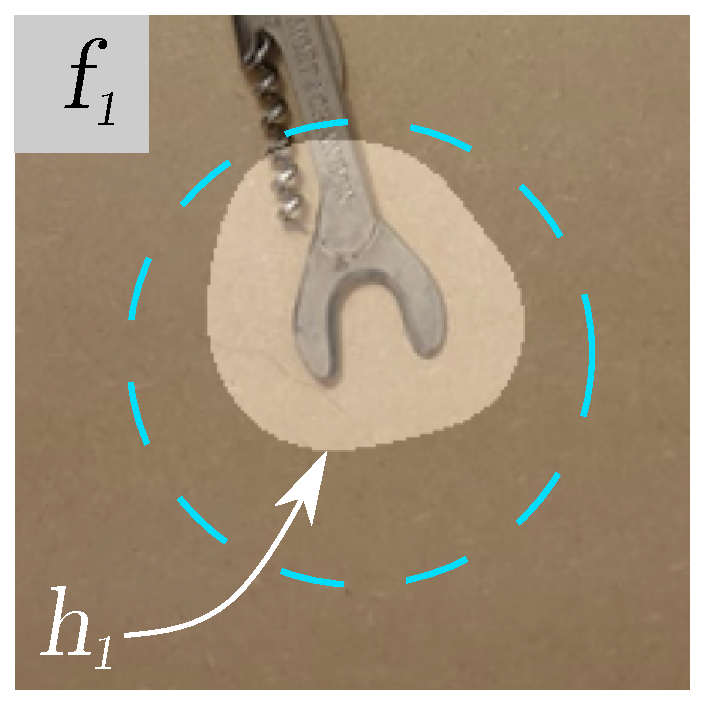
\includegraphics[width=\textwidth]{ch1-diffy/figures/fig_example/scene-h.pdf}
\caption{$f_1$ (close-up)}
\label{fig:sceneh}
    \end{subfigure}\hfil
    \begin{subfigure}{0.25\textwidth}
\includegraphics[width=\textwidth]{ch1-diffy/figures/fig_example/racoon_h.pdf}
\caption{$f_2$ (raccoon's paw)}
\label{fig:raccoonh}    \end{subfigure}\hfil
     \begin{subfigure}{0.25\textwidth}
\includegraphics[width=\textwidth]{ch1-diffy/figures/fig_example/peppers_h.pdf}
\caption{$f_3$ (pepper close-up)}
\label{fig:flowersh}
    \end{subfigure}
\smallskip
     \begin{subfigure}{0.25\textwidth}
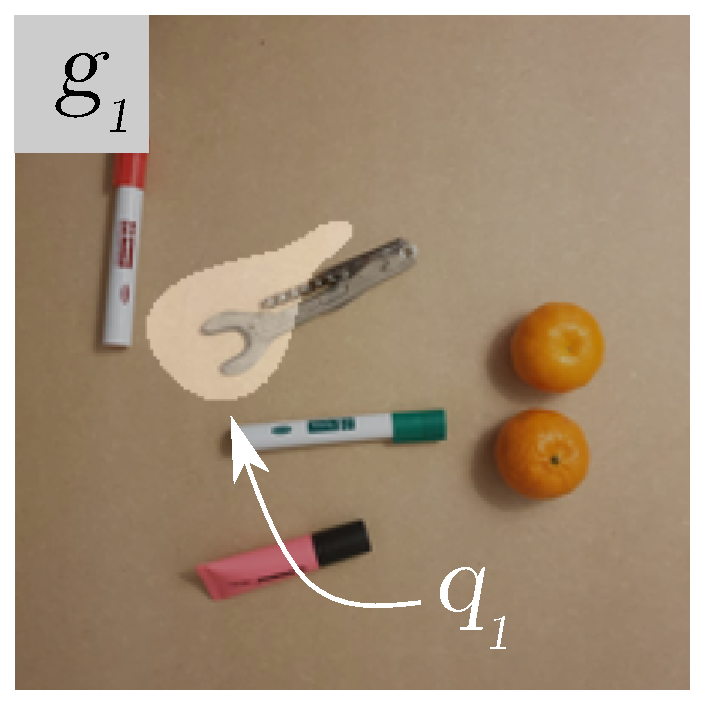
\includegraphics[width=\textwidth]{ch1-diffy/figures/fig_example/scene-q.pdf}
\caption{$g_1$ (scene with multiple objects)}
\label{fig:sceneq}
    \end{subfigure}\hfil
     \begin{subfigure}{0.25\textwidth}
\includegraphics[width=\textwidth]{ch1-diffy/figures/fig_example/racoon_q.pdf}
\caption{$g_2$ (raccoon's abdomen, with natural keystone deformation.)}
\label{fig:raccoonq}
    \end{subfigure}\hfil
     \begin{subfigure}{0.25\textwidth}
\includegraphics[width=\textwidth]{ch1-diffy/figures/fig_example/peppers_q.pdf}
\caption{$g_3$ (peppers among vegetables)}
\label{fig:flowersq}
    \end{subfigure}
\caption[Illustration of Diffy on images.]{\emph{Illustration of $\widehat D_\lambda$ on images.} We compute $\widehat D_\lambda(f_i, g_i)$ and materialize the optimal $h_i$ and $q_i$ selected by \Diffy (with thresholding for visualisation purposes), for $f_i$ and $g_i$ images taken with a smartphone. The mask $\mu$ is illustrated by the dashed circle (in light blue), see \cref{sec:details} for details. The images are taken from different views so as to provide different angles and lighting. \cref{fig:sceneh,fig:sceneq} show a scene of \texttt{objects} and a close-up on one of them (bottle opener). \cref{fig:raccoonh,fig:raccoonq} are taken from images of a raccoon (\texttt{raccoon}). \cref{fig:flowersh,fig:flowersq} are sub-patches from \texttt{peppers}, a scene with vegetables. Notice that $q_i$ visually matches the area highlighted by $h_i$, despite the perspective and scale changes. Additional details are gathered in \cref{sec:illustration}.}
\label{fig:example}
    \end{figure*}

Using tools from functional analysis, we prove that \Diffy behaves as expected when comparing $f$ and $f\circ Q$ (\emph{i.e.}, that it considers these two functions to be close) in the limit of vanishing regularization (\cref{theorem:main-theorem}). We support our theoretical claims with numerical experiments on images.

\paragraph{Outline.} We introduce our new dissimilarity in \cref{sec:dissimilarity}. In \cref{sec:robustness}, we prove that the intuition leading to the definition in \cref{sec:dissimilarity} is well founded and discuss the theoretical properties of the dissimilarity. We then show how to compute the dissimilarity in \cref{sec:computing}: we first show that it has a closed-form expression; we then present and justify an approximation scheme based on Nyström sampling. We illustrate the behavior of the dissimilarity with experiments on images in \cref{sec:experiments}.

\section{The dissimilarity}\label{sec:dissimilarity}

\subsection{Informal derivation of the dissimilarity}\label{sec:informal}

The dissimilarity we describe in this chapter relies on the internal structure of the objects it compares. An efficient way of encoding this structure is to, whenever possible, view objects as maps between an input space and an output space. In this way, we can consider both the values taken by the function and the locations at which these values were taken.

Consider $f$ and $g$ two maps between $\R^d$ and $\R^p$. Our goal is to determine whether there exists a diffeomorphism $Q:\R^d \to \R^d$ such that $g = f \circ Q$. In practice, such transformations could be rigid-body transformations, a non-singular projective transformation or more generally a mild distorsion of the space (such as warping). The goal is thus to find a measure of dissimilarity between $f$ and $g$ that is robust to such diffeomorphisms. We derive such a measure informally in this section around three key ideas.

\paragraph{Change of variable formula.} Integrals offer a natural way to ``eliminate'' a diffeomorphism from a function, via the change of variable formula
\eqals{
\int f(Q(x)) |\nabla Q(x)| \dd x = \int f(x) \dd x.
}
As $|\nabla Q|$ (the determinant of the Jacobian of $Q$) is unknown, we can approximate the above formula with:
\eqal{\label{eq:prob}
\min_{q} \left|\int g(x) q(x) \dd x - \int f(x) \dd x\right|,
} where $q$ lies in a space of functions.

Indeed, when $g = f\circ Q$ for some diffeomorphism $Q$, choosing $q = \vert\nabla Q\vert$ minimizes \eqref{eq:prob}. However, this solution is not unique. Indeed there exist trivial solutions as $q = f / g$, that are irrespective of the existence of a $Q$ such that $g=f\circ Q$ or not.

\paragraph{Range of statistics.} One way of reducing the class of solutions to ones that are relevant to our original question is to study not only how well the weighted integral of $g$ can approximate the integral of $f$, but also require that the same weight approximate a wide class of transformations of $f$. A natural example with inspiration in probability theory is to be able to approximate all moments of $f$, \emph{i.e.}, the integrals of the moments $v_1(f) = f, v_2(f) = f^2, \dots$, or more general statistics. The function $q = f / g$ may match the integral of $v_1(g)$ with that of $v_1(f)$, but cannot work for $v_2$. However, if $g = f\circ Q$, $q = |\nabla Q(x)|$ (the solution we are seeking), satisfies that for any continuous function $v: \R^p \to \R$,
\eqals{
\int v(f(Q(x))) |\nabla Q(x)| \dd x = \int v(f(x)) \dd x.
}
Problem \eqref{eq:prob} is thus replaced by the following one, which also has $q$ as a solution when $g = f \circ Q$:
\eqal{\label{eq:prob2}
\min_q \max_{v \in V} \left|\int v(g(x)) q(x) \dd x - \int v(f(x)) \dd x\right|,
} where $V$ is a rich set of statistics, \emph{e.g.}, continuous integrable functions on $\R^p$.

% %\begin{figure}[t]
% %    \centering
% %    \includegraphics[width=0.35\textwidth]{ch1-diffy/figures/cartoon_export.pdf}
% %    \caption{Illustration of our method. Top: $f$ image with mask $\mu$ (dashed area). Bottom: $g$ is the transformation of $f$ by a diffeomorphism $Q$. Two solutions $q_1$ and $q_2$ are illustrated. $q_1$ (blue, solid line) is obtained with regularization $\lambda_1$. $q_2$ (red, dashed line) is obtained with regularization $\lambda_2 > \lambda_1$. Notice that $q_2$ is a simpler function than $q_1$ (i.e. $\norh{q_2} < \norh{q_1}$) as \Diffy is applied with stronger regularization.}
% %    \label{fig:reg}
% %\end{figure}


\paragraph{Uniformity over regions.} Problem \eqref{eq:prob2} averages the statistics uniformly over the whole space irrespectively of the fact that a witness of $g \neq f \circ Q$ could live in a lower dimensional region. For instance $g$ and $f$ might be non-zero only on a small region of the space, consequently yielding to a relatively small value for \cref{eq:prob2}. To enhance such regions, we choose to integrate with respect to a smooth function $h$, that is chosen adversarially to maximize the dissimilarity between $f$ and $g$.  %We require that for any region of the domain of $f$ and $g$ (encoded by $h$), there exists an equally smooth function $q$ whose induced transformation on $v(g)$ matches that of $h$ on $\phi(f)$.
In other words, we arrive at the following optimization problem:
\eqals{
\max_{h \in \hh_1} \min_{q} \max_{v \in V} \left|\int v(g(x)) q(x) \dd x - \int v(f(x)) h(x) \dd x\right|,
}
where $\hh_1$ is a suitable set of smooth functions.
Again, if $g = f\circ Q$, the above is solved by $q \,=\, h\circ Q \, |\nabla Q|$.



Note that the smoothness of $h$ and $q$ is crucial. On the one hand, the smoothness of $h$ ensures that the considered regions are of interest with respect to the underlying metric on $\R^d$, i.e. they cannot be too close to diracs on pathological sets. On the other, the smoothness of $q$ ensures that the transformations are not matched by ``cherry-picking'' dispersed points on the domain such that the integrals match.


 %\begin{figure*}[ht]
 %    \centering
 %    \begin{subfigure}[b]{0.40\textwidth}
 %        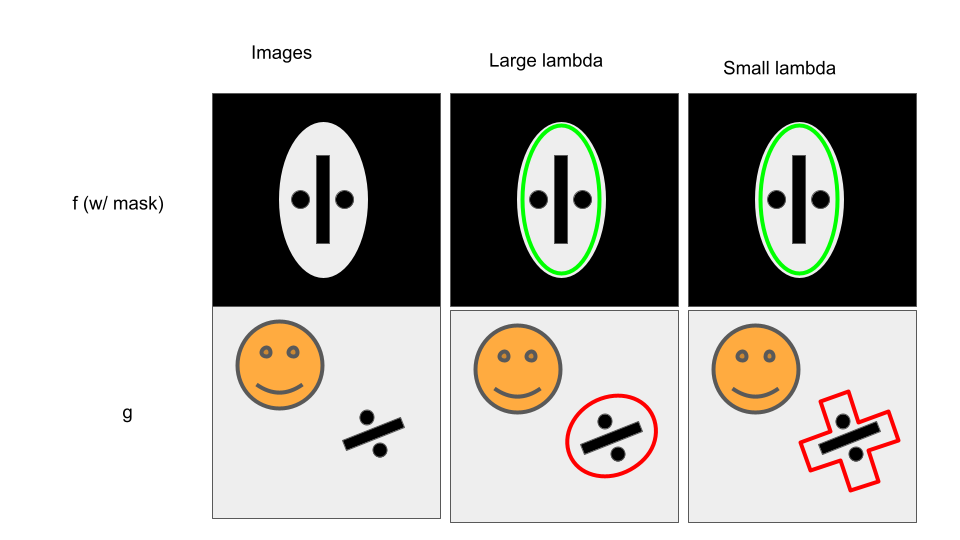
\includegraphics[width=\textwidth]{ch1-diffy/figures/sketch_reg.png}
 %        \caption{When there is a diffeomorphism: regularization ensures that the smoothest solution is found.}
 %    \end{subfigure}\quad
 %    \begin{subfigure}[b]{0.40\textwidth}
 %        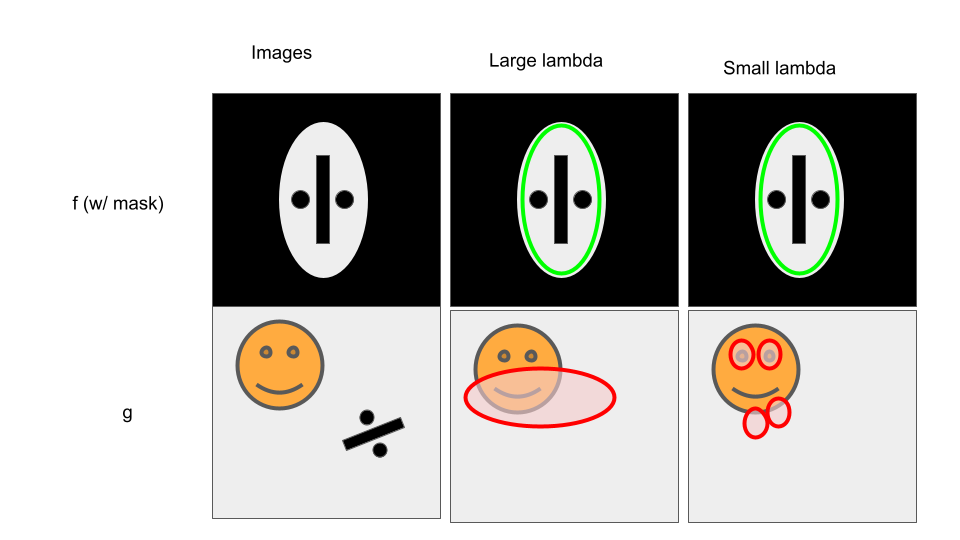
\includegraphics[width=\textwidth]{ch1-diffy/figures/sketch_reg_2.png}
 %        \caption{When there is not a diffeomorphism: regularization is essential to ensure that the distance does not try to find one at all costs!}
 %    \end{subfigure}
 %    \caption{Effect of regularization}
 %    \label{fig:reg}
 %\end{figure*}

\subsection{Definition of the dissimilarity}
Now that we have given the motivation as well as the intuition behind our method, we can formally introduce it.


Let $X \subseteq \R^d$ and $Y \subseteq \R^p$ where $d, p \geq 1$. In this chapter, the objects of interest are maps from $X$ to $Y$. Note that this is quite flexible and can reflect many of the rich types of data considered in image processing, time-series modelling and machine learning. Indeed, an image can be seen as a map from $\R^2$ (the coordinates of the pixels) to $\R^3$ (the color space, RGB for instance). A time-series can be seen as a map from $\R^1$ (time) to $\R^n$ (the space of the sample values).

Let $k_X$ be a reproducing kernel on $X$ with Reproducing Kernel Hilbert Space (RKHS) $\mathcal H$  \cite{aronszajn1950theory} and $k_Y$ be a reproducing kernel on $Y$ with RKHS $\mathcal F$. In particular, we assume that they are bounded.


To conclude, the formalization below allows naturally for the presence of a mask function $\mu$, with the role of focusing the matching process on a subregion of interest of $f$. The role of the mask will be discussed after the definition.


\begin{definition}[Dissimilarity $D_\lambda(f, g)$]\label{def:D}
    Let $\la \geq 0$ and bounded integrable $\mu:\X \to \R$.  For any $f,g:X\to Y$, we define the dissimilarity
\eqal{\label{eq:def-D}
    D_\lambda(f, g) := \max_{\norh{h}\leq 1}\min_{q \in \mathcal H} \Delta_{f,g}(h, q) + \lambda \norh{q}^2
}
where $\Delta_{f, g}(h, q)$ is defined as follows,
\begin{align*}
\Delta_{f, g}(h, q) := \max_{\|v\|_{{\cal F}} \leq 1} &\Big|  \int_X v(g(x))q(x)\dd x-  \int_X v(f(x))\mu(x)h(x)\dd x\Big|^2.
\end{align*}
\end{definition}

\noindent When clear from context, we write $D$ instead of $D_\la$ for the sake of conciseness.

%The reader should easily recognize the construction described in \cref{sec:informal}. We have made the space in which we search for $q$ and $h$ precise: $\hh$, the RHKS of $k_X$. Regularity of $h$ is enforced by searching in the unit ball, while regularity of $q$ is enforced with Tikhonov regularization. This choice allows at the same time to compute the dissimilarity in closed form (see \cref{sec:computing}), while not sacrificing its expressivity (see \cref{sec:approximation}). In particular, to allow a very rich set of statistics that is also manageable from a computational viewpoint, we choose $V$ to be the unit ball of ${\mathcal F}$. For example, if $Y$ is a bounded subset of $\R^p$ and $k_Y$ is chosen as the Laplace kernel $k_Y(y,y') = \exp(-\|y-y'\|)$, then a rescaled version of any infinitely smooth function belongs to $V$ (including in particular all polynomials, smooth probabilities, Fourier basis -- see \cref{app:background} for more details). For the same reason we choose $\hh_1$ to be the unit ball of $\hh$ and we choose also $q \in \hh$.
\cref{fig:example} shows a few examples of the role played by the $h$ and $q$ optimizing the problem in \cref{eq:def-D}.


\begin{figure*}
    \centering
    \begin{subfigure}[t]{0.45\textwidth}
        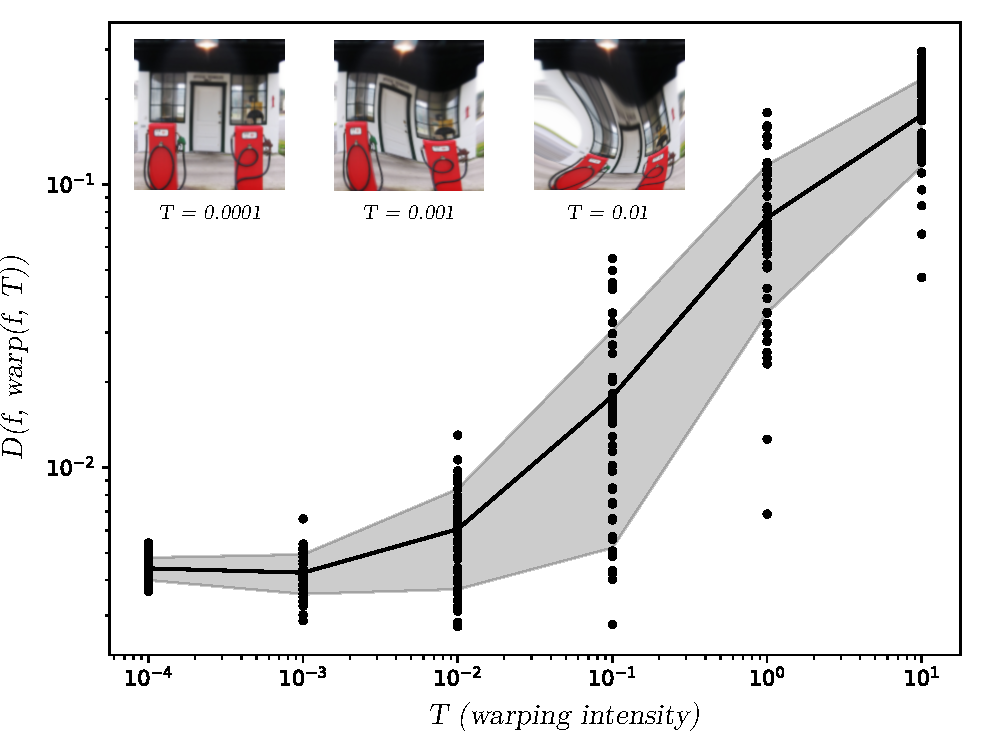
\includegraphics[width=\textwidth]{ch1-diffy/figures/fig_warping/warping_left.pdf}
        \label{fig:warping-left}
        \caption{\emph{$\widehat D_\lambda(f, \text{warp}(f, T))$ as a function of $T$.} We repeat the warp $50$ times ($+$ markers) on the same image and represent average values $\pm$ standard deviation (in grey).}
    \end{subfigure}\qquad
    \begin{subfigure}[t]{0.45\textwidth}
        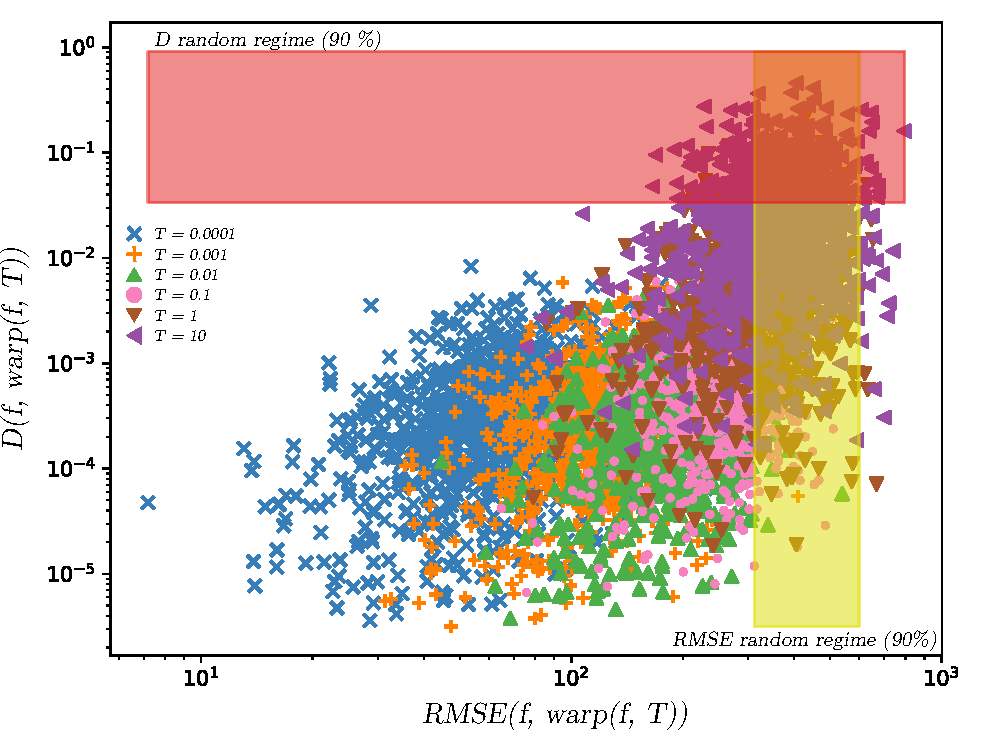
\includegraphics[width=\textwidth]{ch1-diffy/figures/fig_warping/warping_right.pdf}
        \caption{\emph{$\textrm{RMSE}(f, \textrm{warp}(f, T))$ against $\widehat D_\lambda(f, \textrm{warp}(f, T))$ for various values of $T$ and images $f$.} $1000$ images are each warped once for each value of $T$. We represent the random regime for each metric.}
    \end{subfigure}
    \caption[Invariance of Diffy to general diffeomorphisms (warping).]{\emph{Invariance to general diffeomorphisms (warping).} Warping is randomly generated, its intensity controlled by a temperature parameter $T$ (higher $T$ produces, on average, warps with higher displacement norm). In (a): $\widehat D_\la$ stays constant (i.e. invariant to the warps) as long as their norm is not too strong (small T), while RMSE increases exponentially. When $T$ becomes large the transformations become intense (indeed they are non-diffeomorphic) and $\widehat D_\la$ grows to reflect this fact.  In (b): we see that $\widehat D_\la$ stays invariant to warps as long as $T \leq 0.1$ (far from the random regime interval), while the Euclidean distance increases exponentially with $T$, even for small $T$. See \cref{sec:invariance-warping} for more details.}
    \label{fig:warping}
\end{figure*}


\paragraph{The role of the mask $\mu$.} We introduced a function $\mu:X \to \R$ which applies to the term depending on $f$ and $h$. This function is meant to be a mask which focuses the distance on a certain region of $f$, discounting other regions. Such presence is useful in practice, since typically the space $X$ is given by the problem. For example, if we want to use the dissimilarity to check if the content of a given image ($f$) is contained in an image ($g$), the shape $X$ is typically rectangular, while the region of interest is the interior of the image. In this case the mask is useful to avoid the artifacts introduced by the corners. Notice that this addition further breaks the symmetry between $f$ and $g$: $f$ becomes a \emph{reference}, and we search in $g$ for matching statistics. In the experiments, we relied for example on a Blackman Window, a classical window function in signal and image processing (see \cref{sec:details}) to reduce the impact of the corners.



%%%%%%%%%%%%%%%%%%%

\section{Robustness to diffeomorphisms}\label{sec:robustness}


The dissimilarity $D$ is designed (consistently with the derivation in \cref{sec:informal}) to be small when $f$ and $g$ are equal up to a diffeomorphism. The ideal result would be something along the lines of the following \emph{informal} theorem:

\begin{theorem}[Ideal]\label{thm:ideal}
    For any $f: X \to Y$ and any $Q$ diffeomorphism over $X$, $D(f, f\circ Q) \approx 0.$
\end{theorem}

This is of course too much to ask. Indeed, the regularization over the choice of $q$ (which in turn controls the regularity of the jacobian of a hypothetical $Q$) introduces a bias:  even if $g = f \circ Q$, the dissimilarity is not $0$. This bias vanishes if and only if $q^*=0$ (by definiteness of the norm).

However, when the RKHS is assumed to be rich enough and $Q$ and $\mu$ are regular enough, then we have the following result. Before stating it, we recall that the Laplace kernel $k_X(x,x^\prime) = \exp(-\|x-x^\prime\|)$ belongs to the more general family of Sobolev kernels \cite{wendland2004scattered}. In particular, it corresponds to the Sobolev kernel of smoothness $m$, with $m = (d+1)/2$, where $d$ is the dimension of $X \subset \R^d$.
\begin{theorem}\label{theorem:main-theorem}
Let $X \subset \R^d$ be an open bounded set with Lipschitz boundary. Let $\mu \in C^\infty(\R^d)$ with compact support $\Omega \subset X$. Choose $k_X$ to be a Sobolev kernel of smoothness $m$, with $m > d/2$. Then for any $C^{m+1}$ diffeomorphism $Q$ on $\R^d$ satisfying $Q^{-1}(\Omega) \subset X$, we have that
\eqals{
 D_\la(f, f \circ Q) ~~\leq~~ \lambda ~ C^2_{\mu} C^2_{Q} \qquad \forall f\, \textrm{measurable},
}
where $C_\mu = \|\mu\|_{H^m(\R^d)}$, and $C_Q$ is defined in \cref{eq:def-CQ} in \cref{sec:general-theorem} and depends only on $\Omega, X, Q, d, m$.
\end{theorem}
%%%%%%
The theorem above is a special case of \cref{thm:general-theorem}, presented in \cref{sec:general-theorem}. There we prove the more general result: $D_\lambda(f,g) \leq \lambda C^2_{\mu} C^2_{Q}$, for all measurable $f, g$ that satisfy $g(x) = (f \circ Q)(x)$, only in the region not canceled by the mask, \emph{i.e.}, $\forall x \in Q^{-1}(\Omega)$.



A first consequence of \cref{theorem:main-theorem} is that the regularization parameter $\lambda$ controls the threshold to decide whenever $g \approx f \circ Q$. In particular, we easily see that $D_\la(f, f \circ Q) \to 0$, when $\la \to 0$. This result confirms that in the limit where the regularization vanishes, so does the bias and we have the result we would have imagined à la \cref{thm:ideal}. We will see in \cref{sec:approximation} that $\la$ has also an important role in controlling the approximation error of $D(f,g)$. This shows that $\la$ controls a similar bias-variance trade-off as in classical kernel supervised learning \cite{shawe-taylor2004}.

To illustrate  the dependence of $C_Q$ with respect to $Q$, in the following example we explicitly compute $C_Q$ for an interesting class of diffeomorphisms.

\begin{example}[Magnitude of $C_Q$ for rigid transforms]\label{ex:diffeo}
Let $X$ be the unit ball in $\R^d$ and let $\mu$ be a mask supported on $\Omega$, the ball of radius $r < 1$. We consider the diffeomorphisms $Q(x) = \alpha R x$, with $R$ a unitary matrix and $r < \alpha < 1/r$. We use the Laplace kernel $k_X(x,x^\prime) = \exp(-\|x-x^\prime\|)$ for $k_X$ (analogously for $k_Y$).
Then, we compute explicitly the bound in \cref{eq:def-CQ}, since the Laplace kernel corresponds to Sobolev kernel with exponent $m = (d+1)/2$, obtaining
$$C_Q ~~\leq~~ C_0 \left(\frac{\alpha}{\min(\alpha,1) - r}\right)^{m+d/2}\alpha^d (1 + \alpha + \alpha^m).$$
\end{example}
\begin{remark}
By seeing data points as functions, we are able to efficiently reason about them. Hence, since data points are continuous objects, $d=\dim(X)$, the dimensions of $X$, and not the number of pixels, which we denote $N$ below. Indeed, $X$ is low-dimensional by nature: for images, $d=2$ since images are 2-d objects, while $N$ could be very large. This way, the dimensional dependence of $C_Q$ is very reasonable. In the extreme case where we consider time series of point clouds (for example, brain scans through time), $d = 4$ (time $+$ 3 spatial coordinates). If we consider a scale change range of $50\%$, then $C_Q$ is of the order of $3/2^4 \approx 5$. We emphasize that $C_Q$ is not related to the number of samples (for images, the number of pixels) used to compute DID in practice.
\end{remark}
\subsection{Discussion on the discriminatory power of $D_\la$} \label{sec:discussion-selectivity}
In \cref{theorem:main-theorem}, we proved that when $g = f \circ Q$ for some diffeomorphism $Q$, then $D(f,g)$ is small, i.e. that the dissimilarity is essentially invariant to the diffeomorphisms. However, to fully characterize the properties of the proposed dissimilarity it would be interesting to study also its discriminatory power, i.e. the fact that $D(f,g)$ is small {\em only if} there exists a diffeomorphism $Q$ such that $g = f \circ Q$. \cref{fig:warping} investigates this question from the empirical perspective. The details of these experiments are reported in \cref{sec:experiments} (and further explored in \cref{app:additional-experiments}). They show that, \Diffy is very robust to significant transformations $f\circ Q$ of the original signal $f$. Additionally we observe that $D_\la$ is very discriminative, in contrast to less diffeomorphism invariant metrics such as the euclidean distance, when comparing $D_\la(f,f\circ Q)$ with $D_\la(f,g)$ for a random signal $g$. We care to point out however, that the theoretical analysis of \Diffy's the discriminative abilities is beyond the scope of this chapter (whose aim is to introduce the discrepancy and study its invariance properties) and we postpone it to future research.

%%%%%% However, the experimental analysis performed in \cref{sec:experiments} and further in \cref{app:additional-experiments} strongly supports it.



%%%%%%%%%%%%%%%%%%%%%

\section{Computing the dissimilarity}\label{sec:computing}

Before deriving the closed form solution for $D_\la$, we need to recall some basic properties of kernels. Reproducing kernels and RKHSs satisfy the so called {\em reproducing property}, i.e. There exists a map $\psi:X \to \hh$ such that, for any $f \in \hh$ and $x \in X$, it holds that $f(x) = \scal{f}{\psi(x)}_\hh$, where $\scal{\cdot}{\cdot}_\hh$ is the scalar product associated to the RKHS $\hh$. Moreover $k_X(x,x^\prime) = \scal{\psi(x)}{\psi(x^\prime)}_{\hh}$, for all $x,x^\prime \in X$. The same holds for $k_Y$ and $\cal F$. i.e., there exists $\Phi:Y \to {\cal F}$ such that $v(y) = \scal{v}{\Phi(y)}_{\cal F}$ for all $v \in {\cal F}, y \in Y$ and $k_Y(y,y^\prime) = \scal{\Phi(y)}{\Phi(y^\prime)}$ for all $y,y^\prime \in Y$, where $\scal{\cdot}{\cdot}_{\cal F}$ is the inner product associated to ${\cal F}$. In particular, note that, since we assumed that $k_X, k_Y$ are bounded kernels, then there exist two constants $\kappa_X, \kappa_Y$ such that $\sup_{x \in X} \|\psi(x)\|_{\hh} \leq \kappa_X$ and analogously $\sup_{y \in Y} \|\Phi(y)\|_{\cal F} \leq \kappa_Y$.



\subsection{Closed form solution}
In \cref{def:D}, we define $D_\lambda(f,g)$ as an optimization problem in $\hh \times \hh$. In fact, this optimization problem has a closed-form solution, as the solution of an eigenvalue problem of an operator between $\hh$ and $\mathcal F$ as derived in \cref{eq:cl-form-eig-Dla}. We introduce the relevant objects and prove \cref{theorem:closed-form}.

\begin{definition}[Operators $F_\mu$, $G$]\label{def:operatorsFG}
Given $f, g: X \to Y$, the feature map $\Phi: Y\to \mathcal F$ and the mask function $\mu:X \to \R$, define the linear operators $F_\mu, G:\hh \to {\cal F}$ as follows:
\eqal{
F_\mu &= \int_X \Phi(f(x)) \otimes \psi(x) \mu(x) \dd x, \\ G~&= \int_X \Phi(g(x)) \otimes \psi(x) \dd x.
}
\end{definition}

\cref{def:operatorsFG} is a compact notation for the the integral operators in the RKHS. Noticing that we can rewrite $\Delta_{f,g}$ (see below) as a function of $F_\mu$ and $G$ is key to deriving the closed-form expression and the finite-dimensional approximation in \cref{eq:widehatA,eq:widehatB}, that can be computed in practice.

When $X$ is a bounded set, the two operators above are trace class and, by the representer property  $\scal{v}{F_\mu h}_{\cal F} = \int_X v(f(x)) h(x) \mu(x) dx$ and also $\scal{v}{G q}_{\cal F} = \int_X v(f(x)) q(x) dx$ (see \cref{lm:explicit-Fmu-G} in \cref{sec:additional-proofs} for a detailed proof). Using this result and considering the linearity of $\scal{\cdot}{\cdot}_{\cal F}$ and the variational characterization of the Hilbert norm (i.e. $\|u\|_{\cal F} = \max_{\|v\|_{\cal F} \leq 1} |\scal{v}{u}_{\cal F}|$), we have
\eqals{
\Delta_{f,g}(h,q) & = \|F_\mu h - G q\|_{\cal F}^2,
}
for any $h, q \in \hh$. From which we characterize $D_\lambda$ as
\eqal{
D_\lambda(f, g) = \max_{\norh{h}\leq 1} \min_{q\in\hh} \norf{F_\mu h - G q}^2 + \lambda \norh{q}^2.
}
To conclude, note that the optimization problem in the equation above has a closed-form expression in terms of the operatorial norm of an operator depending on $F_\mu$ and $G$. All the reasoning above is formalized below.
\begin{theorem}[Closed-form solution]\label{theorem:closed-form}
Let $X \subset \R^d$ be an open bounded set. Using the notations above, we have:
\eqal{\label{eq:cl-form-eig-Dla}
D_\lambda(f, g) = \lambda\norop{(GG^* + \lambda I)^{-1/2}F_\mu}^2.
}
\end{theorem}
The proof of \cref{theorem:closed-form} comes from identifying the inner optimization problem as a linear regression problem, and the the outer maximization problem as an eigenproblem. The complete proof is presented in \cref{sec:proof-closed-form}.

\begin{figure}[t]
    \centering
    \includegraphics[width=0.8\textwidth]{ch1-diffy/figures/fig_rotation/rotation}
    \caption[Invariance of Diffy to rotation.]{\emph{Invariance to rotation.} We consider a patch $f$ (size $100\times 100$) of a larger scene (\texttt{peppers.jpeg}) and compare it to its rotated versions $\text{rotate}(f, \alpha)$, where $\alpha$ is an angle. $D(f, \text{rotate}(f, \alpha))$ is represented with $+$ symbols and $\textrm{RMSE}(f, \text{rotate}(f, \alpha))$ with $\times$ symbols. Random regimes are represented by shaded areas (see text). Both $\widehat D_\la$ and the RMSE seem constant as a function of $\alpha$ (although with $\alpha=0$ or $\alpha=180$ a smaller value is achieved). However, the RMSE of the rotated patches falls in (or close to) the confidence interval, making them indistinguishable from random patches from the same image. $\widehat D_\la$ takes values that are over $10 \times$ smaller for rotated patches that for random patches. Hence, \Diffy is invariant to rotation, whereas RMSE is constant (for $\alpha > 0$). Here $\la = 10^{-6}$. See \cref{sec:invariance-rotation} for more details.}
    \label{fig:rotation}
\end{figure}

\section{Approximate computation}\label{sec:approximation}

Although \cref{theorem:closed-form} gives a closed-form expression of $D_\lambda(f,g)$, $F_\mu$ and $G$ are defined as integral operators between infinite dimensional Hilbert spaces. In practice, we only have access to a discretization of $f$ and $g$ (e.g. an image is a discretized spatial signal represented by $N$ pixels). A first natural approximation is thus to replace the integral with an empirical counterpart. This estimate is then a sum of rank-one operators between $\mathcal H$ and $\mathcal F$. To reduce the computational cost, while keeping good accuracy, we can then further approximate it using Nyström methods for kernels. The resulting estimator is $\widehat{D}_\la$ presented in \cref{eq:widehatD-finite-dimensional}, its convergence to $D_\la$ is studied in \cref{thm:appr-error-widehatD}.


\paragraph{Quadrature approximation.}

We replace $F_\mu$ with an estimator $F_{\mu, N}$ and $G$ with an estimator $G_N$:
\eqal{
F_{\mu, N} &= \frac{v_X}{N}\sum_{i=1}^N \Phi(f(x_i)) \otimes \psi(x_i) \mu(x_i)\label{eq:F-sum}\\
G_{N} &= \frac{v_X}{N}\sum_{i=1}^N \Phi(g(x_i)) \otimes \psi(x_i),\label{eq:G-sum}
}
where $v_X := \int_X \dd x$ is the volume of the domain $X$.
Note that the set of $\lbrace x_1, \ldots, x_N \rbrace$ can be chosen at random or arbitrarily to best approximate the integrals. $F$ and $G$ can be approximated using different points. In practice, they are often given as the positions of pixels of images, sample times of a time series.

\paragraph{Nyström approximation.}

From the previous section, it is clear that $\rank{F_{\mu, N}} \leq N$ and $\rank{G_N} \leq N$. This justifies using the low-rank approximations we introduce in this section. It is possible to further reduce the rank of the matrices, while keeping a good accuracy, by using the so-called {\em Nystr\"om approximation} \cite{williams2001using,drineas2005nystrom,rudi2015less}.

Let $M_X, M_Y \in \N$ and choose the set of points $\widetilde{X} = \lbrace \widetilde x_1, \ldots, \widetilde x_{M_X}\rbrace \subset X$ and $\widetilde{Y} = \lbrace \widetilde y_1, \ldots, \widetilde y_{M_Y} \} \subset Y$. The Nystr\"om approximation of a vector $v \in \hh$ is the projected vector $P_{\tilde{X}} v$, where $P_{\tilde{X}} :\hh \to \hh$ is the projection operator with range corresponding to $\textrm{span} \{\psi(\tilde{x}_1),\dots,\psi(\tilde{x}_{M_X})\}$. Note, in particular, that $P_{\tilde{X}}$ has rank $M_X$ when $k_X$ is universal. $P_{\tilde{Y}}: {\cal F} \to {\cal F}$ on $\tilde{Y}$ in defined analogously.


\paragraph{Combining the two approximations.}
Assume in this section, that the kernels of choice are universal (as, e.g., the Laplacian or the Gaussian kernel).
Let $P_{\tilde{X}}:\hh \to \hh$ be the projection operator associated to the Nystr\"om points on $X$ and $P_{\tilde{Y}}$ the one associated to the Nystr\"om point on $Y$. Combining the two approximations, we define the following estimator for $D_\la$,
\eqals{
\widehat{D}_\la(f,g) := \la \|(P_{\tilde{Y}} G_N P_{\tilde{X}} G_N^*P_{\tilde{Y}} + \la)^{-\frac{1}{2}} P_{\tilde{Y}} F_{\mu, N} P_{\tilde{X}} \|^2_{\mathrm{op}}.
}
Note, however, that $\widehat{D}_\la(f,g)$ has a finite dimensional characterization that we are going to derive now.
Let $K_{\widetilde Y f} \in \mathbb R^{M_Y \times N}$ the matrix defined by $(K_{\widetilde Y f})_{i, j} = k_Y(\widetilde y_i, f(x_j))$, $K_{\widetilde Y g}$ in an analogous way, and finally, $K_{X \widetilde X}\in\R^{N \times M_X}$ the matrix defined by $(K_{X\widetilde X})_{i, j} = K_X(x_i, \widetilde x_j)$. Let $\widehat \mu = \left[ \mu(x_1), \ldots, \mu(x_{M_X})\right]$ and $R_{\widetilde X} \in\R^{M_X \times M_X}$ be the upper-triangular Cholesky decomposition of $K_{\widetilde X \widetilde X}$ defined by $(K_{\widetilde X \widetilde X})_{ij} = k_X(\widetilde x_i, \widetilde x_j)$. Analogously, define $K_{\widetilde Y \widetilde Y}$ and define $R_{\widetilde Y}\in\R^{M_Y \times M_Y}$ its Cholesky decomposition. Note that the decomposition exists since the kernel $k_X$ is universal and so the kernel matrix $K_{\tilde{X},\tilde{X}}$ is invertible.


We introduce the following operators $\widehat{A}, \widehat{B} \in \R^{M_Y \times M_X}$, which are the finite dimensional representations in appropriate spaces $\R^{M_X}, \R^{M_Y}$ of, respectively, $\tilde{P}_Y F_{\mu, N} \tilde{P}_X$ and $\tilde{P}_Y G_N \tilde{P}_X$:
\eqal{
\widehat{A} ~&=~ \frac{v_X}{N} R_{\widetilde Y}^{-T} K_{\widetilde Y f} \diag{\widehat \mu} K_{X\widetilde X} R_{\widetilde X}^{-1},\label{eq:widehatA}\\
\widehat{B} ~&=~ \frac{v_X}{N} R_{\widetilde Y}^{-T} K_{\widetilde Y g} K_{X\widetilde X} R_{\widetilde X}^{-1}. \label{eq:widehatB}
}
In particular, we have the following characterization for $\widehat{D}_\la$.
\begin{lemma}\label{lm:widehatD}
With the notation above,
\eqal{\label{eq:widehatD-finite-dimensional}
\widehat{D}_\la(f,g) = \la \|\widehat{A}^* (\widehat{B} \widehat{B}^* + \la I)^{-1} \widehat{A}\|_{\mathrm{op}}.
}
\end{lemma}

Note that, in practice, $\widetilde X$ and $\widetilde Y$ can be chosen either deterministically, e.g. on a grid, or randomly. Now, we provide a bound on the approximation error associated to $\widehat{D}_\la(f,g)$. We assume that the $N$ points in $x_1,\dots, x_N$ are sampled independently and uniformly at random in $X$ and, moreover, that the $M_X$ points in $\widetilde{X}$ and the $M_Y$ points in $\widetilde{Y}$ are sampled independently and uniformly at random in, respectively, $X, Y$ (similar result can be derived for a grid).
\begin{theorem}\label{thm:appr-error-widehatD}
Let $\delta \in (0,1)$. Let $X \subset \R^d, Y \subset \R^p$ be bounded sets and $k_X, k_Y$ be Sobolev kernels with smoothness, respectively, $s + d/2$ and $z+p/2$, for some $s,z > 0$. There exists two constants $c_1, c_2$ s. t., when $M_X \geq c_1$ and $M_Y \geq c_2$, then the following holds with probability $1-\delta$,
$$|\widehat{D}_\la(f,g) - D_\la(f,g)| \leq c\left(\tfrac{\log\frac{1}{\delta}}{\la\sqrt{N}} + \tfrac{\left(\log \frac{M_X}{\delta}\right)^{\alpha}}{\la M_X^{s/d}} + \tfrac{\left(\log\frac{M_Y}{\delta}\right)^{\beta}}{\la M_Y^{z/p}}\right),$$
for any measurable $f,g : X \to Y$, where $\widehat{D}_\la(f,g)$ is defined as in \cref{eq:widehatD-finite-dimensional}. Here $c_1, c_2, c$ depend only on $X, Y, \mu, s, z, d, p$, while $\alpha = s/d+1/2$, $\beta = z/p+1/2$.
\end{theorem}

The theorem above shows that the estimation error of $\widehat{D}_\la$ with respect to $D_\la$ goes to $0$ when $N, M_X, M_Y \to \infty$. On the contrary, the error diverges in $\la$. This is in accordance with the fact that the error is of variance type and shows that $\la$ plays the role of a regularization parameter. The bound shows also that, when $s \gg d$ and $z \gg p$, i.e. when we are choosing very smooth Sobolev kernels, the decay rate of the error in $M_X$ and $M_Y$ is faster. For example, if we choose $s = r d$, $z = r p$, for some $r > 0$, then choosing $M_X = M_Y =  O(N^{r/2})$ leads to the rate
$$ |\widehat{D}_\la(f,g) - D_\la(f,g)| = O\left(\frac{1}{\la \sqrt{N}}\right).$$

\paragraph{On the choice of $\la$.}
To conclude, a choice of $\la$ as $\la = N^{-1/4}$ guarantees a final convergence rate of $\widehat{D}_\la$ to $D_\la$ in the order of $N^{-1/4}$ and, together with \cref{theorem:main-theorem} a level of invariance to diffeomorphism for $\widehat{D}_\la$ of the order
$$\widehat{D}_\la(f, f \circ Q) = O(N^{-1/4} C_\mu^2 C_Q^2),$$
which can become a statistically significant threshold to decide if, in practice $f \approx g$ up to diffeomorphism.
Clearly the choice of $r,s$ while reducing the number of Nystr\"om points required in the approximation (with important computational implications that we see below) increases the constant $C_Q$ as shown, e.g., in \cref{ex:diffeo}, where $m = s + d/2$.


%%%%%{\color{red}\bf[Algorithm?]}

\paragraph{Algorithm and computational complexity.}
The final form of the empirical estimator $\widehat{D}_\la$ is \cref{eq:widehatD-finite-dimensional}. An efficient algorithm to compute it is, for instance, (1) first computing the matrices $\widehat{A}$ and $\widehat{B}$, then the inverse $\widehat{C} = (\widehat{B}\widehat{B}^* + \la)^{-1}$ and finally compute the largest eigenvalue of $\widehat{A}^* \widehat{C} \widehat{A}$ via a power iteration method \cite{trefethen1997numerical}. %that is a method based on matrix vector products. In particular this last step avoids to compute explicitly the product of the three matrices, $\widehat{A}^* \widehat{C} \widehat{A} v = \widehat{A}^* (\widehat{C} (\widehat{A} v))$.

Assuming that (a) the cost of one kernel computation in $\R^d$ is $O(d)$ (as in the case of any translation invariant kernel as the Laplace kernel) (b) $M_X \leq N$ and $M_Y \leq N$ (which is reasonable in light of \cref{thm:appr-error-widehatD}), then the cost of computing $\widehat{D}_\la$ with the algorithm above is
$O(d N M_X + p N M_Y + M_XM_Y^2 + M_X^3 + M_Y^3)$.
Choosing the parameters, as in the discussion after \cref{thm:appr-error-widehatD}, with $r = 1$, would lead to a total computational cost of
$O(N^{3/2}(p+d)).$

Computing \Diffy between different pairs of data-points can easily be parallelized as each computation relies on matrix-vector products and matrix inversions.

\paragraph{Choice of kernel hyperparameters.}
As in any kernel-based method, selecting kernel hyper-parameters is important. The usual considerations apply: we advise cross-validation should be used to choose hyper-parameters (such as the bandwith). We do not discuss this further for space considerations.

In the theoretical analysis above, the rates in $N$ hold for any parameter of the kernel, but constants depend on the chosen parameters. This is typical of the Sobolev analysis technique, where the important parameter is the kernel regularity $m$, which corresponds to the differentiability class of the diffeormorphisms one aims to capture.

Finally, the method introduced is empirically quite robust to the choice of parameters.

 %Here we study an efficient strategy to compute it and its computational complexity. Denote $T(d)$ the cost of one kernel evaluation between two points in $\R^d$ (e.g. for the Laplace kernel $T(d) = O(d)$).

 %\textbf{Offline pre-computation~}

 %$R_{\widetilde X}$ is constructed by first computing $K_{\widetilde X\widetilde X}$ in $O(T(d)M_X^2)$ time, then a Cholesky decomposition computation in $O(M_X^3)$ time, for a total ost of $O(T(d)M_X^2 + M_X^3)$. Similarly, computing $R_{\widetilde Y}$ costs $O(T(p)M_Y^2 + M_Y^3)$.  Finally, computing $K_{X\widetilde X}$ costs $O(T(d)M_XN)$.

 %Thus, the computations that can be done offline cost: $O(T(d)M_X(M_X + N) + T(p)M_Y^2 + M_X^3 + M_Y^3)$.

\begin{figure}[t]
    \centering
    \includegraphics[width=0.8\textwidth]{ch1-diffy/figures/fig_regularization/regularization.pdf}
    \caption[Effect of regularization on Diffy.]{\emph{Effect of regularization.} We consider the same image and setting as in \cref{fig:warping} and vary $T$ and $\lambda$ (shaded areas are std deviation over $50$ warps). Observe: (1) $\widehat D_\la$ increases as a function of $T$ (as the norm of the diffeomorphism increases); (2) $\widehat D_\la$ is  proportional to $\lambda$. Both of these phenomena are predicted by \cref{theorem:main-theorem}. See \cref{sec:regularization} for more details.}
    \label{fig:regularization}
\end{figure}


 %$\widehat F$ (and $\widehat G$) can be computed in  $O(M_Y^2 N + NM_XM_Y + M_YM_X^2)$ time. This assumes that the computation is done from right to left. If it is done from left to right, then it becomes $O(M_X^2N + N M_XM_Y + M_XM_Y^2)$, which reduces the complexity in $M_Y$. Depending on the application, $M_X$ or $M_Y$ can tend to be larger and in this case one of the orders is advantageous.

 %The inverse of $\widehat G \widehat G^* + \lambda I$ is computed in $O(M_X^3)$ time, and its product with $\widehat F_\mu$ and $\widehat F_\mu^*$ is $O(M_X^2M_Y + M_Y^2M_X)$.


 %Finally, using a power iteration algorithm
 %\cite{trefethen1997numerical} to compute the operator norm of the computed $M_X \times M_X$ matrix is (naïvely) in $O(kM_X^3)$, where the algorithm does $k$ iterations. If $M_Y \ll M_X$ then we can permute terms in the operator norm and reduce the computation to $O(kM_Y^3)$.

 %In the online phase of the algorithm, that is when we compute $\widehat D_\lambda(f, g)$ for many pairs $(f, g)$, the complexity is of order $O(NM_XM_Y + N\max(M_X, M_Y)^2)$. As we hinted above, this complexity can be reduced by adapting the order of operations and the computation to the problem, i.e. to the relative sizes of $M_X$, $M_Y$ and $N$.



%%%%%%%%%%%%%%%


\section{Experiments}\label{sec:experiments}

This section investigates the empirical performance of \Diffy. We observe that, in line with our results in \cref{theorem:main-theorem}, when $g=f\circ Q$ the resulting $D_\la$ is small, while it is consistently large for signals that are not diffeomorphic versions of $f$.


\subsection{Implementation details}\label{sec:details}

We implemented $\widehat{D}_\la$ as in \cref{eq:widehatD-finite-dimensional} as described in the end of \cref{sec:approximation} using standard linear algebra routines such as matrix and matrix-vector products, matrix inversions, and eigendecompositions. The Python source code used for the experiments presented here is freely available at \href{https://github.com/theophilec/diffy}{https://github.com/theophilec/diffy}, depends on Numpy and Pytorch and supports using GPUs.

\paragraph{Normalization.}
In practice we normalize $\widehat A$ and $\widehat B$ by their operator norms $\norop{\widehat A}$ and $\norop{\widehat B}$. This normalizes $D_\lambda$ between $0$ and $1$ and makes interpretation easier.

\paragraph{Choice of mask.}
We choose $\mu$ to be a Blackman window, a standard windowing function in image processing. In 1-D, the Blackman window is defined for any $0 \leq t \leq 1$ as:
$\mu(t) = 0.42 - 0.5\cos(2\pi t) + 0.08 \cos(4\pi t)$ \cite{oppenheim99}.
We generalize it to higher-dimension by considering its tensor-product over dimensions.

\paragraph{Choice of kernel.}
Because we work with images in the experiments we present, $X = \R^2$ (coordinate space) and $Y = \R^3$ (color space). We consider the Gaussian kernel defined as $k(x, x^\prime) = \exp(- \|x - x^\prime\|^2/(2\sigma^2))$ on $X$ and the Laplace kernel defined as $k(y, y^\prime) = \exp(-a \| y - y^\prime \|)$ on $Y$. For the experiments presented in this chapter, unless otherwise stated, \Diffy has parameters: $M_X = 100$, $M_Y = 16^3$, $\sigma = 1/6$ and $a=5$.

\paragraph{Datasets.}
We rely on images from Imagenet (more precisely from the \texttt{Imagenette} subset), example images from the Matlab software (\texttt{peppers}), and finally images taken with our personal devices for illustrations (\texttt{raccoon, flowers, objects}). All images are made available with the source code.

\paragraph{Diffeomorphism generation.} Diffeomorphism are obtained either by affine transformations or by generating warpings. In particular, for warpings, we use the code from \cite{wyartdiffeo}. We generate random transformations of images by displacing each of its coordinates independently (while enforcing zero displacement at the edge of the grid) then interpolating the colors.  We choose the standard deviation of the displacements of each pixel so as to obtain a transformation of given (average) displacement norm. This can be controlled by two parameters $T$ (a temperature, between $10^{-4}$ and $10^1$) and $c$ (a cut-off parameter, taking $c=2$). We denote $\text{warp}(f, T)$ such a (random) warp. Examples of warps for various $T$ parameters (and samples) are provided in \cref{sec:appendix-warping}.

\subsection{Illustrative examples}\label{sec:illustration}

In \cref{fig:example}, we show how the $h$ and $q$ that optimize \Diffy concentrate on related regions on for different scenes which which are related by a diffeomorphism, in particular rigid-body and perspective for \texttt{objects} and keystone deformation for \texttt{raccoon}. We present supplementary illustrative examples in \cref{app:additional-experiments}.

\subsection{Invariance to warping}\label{sec:invariance-warping}
Diffeomorphisms (even infinitely regular) are a much wider class of transformations than rigid body transformations such as scale, rotation and translation (or combinations thereof). In this experiment (\cref{fig:warping}), we evaluating \Diffy's behavior against a wide family of transformations (we call warps). Consider $f$ an image from $\texttt{Imagenette}$. For $T = 10^{k}$ for $-4 \leq k \leq 2$ and various images, we evaluate $\widehat D_\lambda(f, \text{warp}(f, T))$ as well as $\textrm{RMSE}(f, \text{warp}(f, T))$. We compare the values observed to $\widehat D_\la(f, g)$ and $\textrm{RMSE}(f, g)$ for random images $f$ and $g$. We call this the \emph{random regime} ($90\%$ confidence interval). Finally, we look at the performance of \Diffy on a fixed image (gas station), with repeating warps. \cref{fig:warping} shows that \Diffy is invariant to diffeomorphic warping for $T \leq 10^{-1}$ whereas the Euclidean distance increases exponentially with $T$ (making $\text{warp}(f, T)$ indistinguishable from $g$, a random image).

\subsection{Invariance to rotation}\label{sec:invariance-rotation}
The \texttt{peppers} image is often used to demonstrate image registration techniques. In this experiment (see \cref{fig:rotation}) we show that \Diffy is invariant to rotation using patches taken from it. Consider $f$ a patch from \texttt{peppers} and $g = \text{rotate}(f, \alpha)$, rotated version of $f$ by angle $\alpha$ (in practice, we rotate a larger patch then crop to avoid artifacts). We then compare $D(f, \text{rotate}(f, \alpha))$ and $\textrm{RMSE}(f, \text{rotate}(f, \alpha))$. We show that while the Euclidean distance is \emph{constant} for $\alpha \neq 0$, \Diffy is \emph{invariant}. We compare \Diffy's and the Euclidean distance values with their values for random patches from the image. As before, we call this the \emph{random regime} ($90\%$ confidence interval). This shows that the Euclidean distance is not able to distinguish between a random patch and a rotated version of the same patch, while \Diffy can. See \cref{fig:rotation} for the results of the experiments.

\subsection{Effect of regularization}\label{sec:regularization}
In order to understand the effect of regularization, we reuse the setup from \cref{sec:invariance-warping} with a single image, with varying $\lambda$. In \cref{fig:regularization}, we observe two phenomena: (1) as $T$ increases, so does $D$; (2) as $\lambda$ decreases, so does $D$. This shows that \Diffy behaves close to what is predicted by \cref{theorem:main-theorem}. Indeed, $D$ seems proportional to $\lambda$. Also, as $T$ increases, so does the norm of the transformation between $f$ and $\text{warp}(f, T)$. This makes the upper bound of \cref{theorem:main-theorem} increase in turn.

% todo
%\begin{subappendices}
%\section{Background} \label{app:background}


We recall here the classical version of change of variable theorem for $\R^d$, see e.g. Thm. 40.7 of \citet{aliprantis1998principles}.
\begin{theorem}[Change of Variables]\label{thm:change-of-variable}
Let $V$ be an open set in $\R^d$ and $Q:\R^d \to \R^d$ be an injective continuosly differentiable map. Let $f \in L^1(V)$. Denote by $\nabla Q(x) \in \R^{d\times d}$ the gradient of $Q$ for any $x \in \R^d$. Then, we have
$$\int_{Q^{-1}(V)} f(Q(x)) |\nabla Q(x)| dx = \int_{V} f(y) dy. $$
\end{theorem}


\subsection{Sobolev spaces}

We recall some basic properties of Sobolev spaces. The Sobolev space $H^m(Z)$ for $m > 0$ and an open set $Z \subseteq \R^d$ is defined as follows \cite{adams2003sobolev}
$$H^m(Z) = \big\{f \in L^2(\R^d) ~\big|~ \|f\|_{H^m(Z)}\big\} < \infty\big\}, \quad \|f\|^2_{H^m(Z)} = \sum_{\alpha_1+\dots+\alpha_d \leq m} \int_{Z} \left|\frac{\partial^{\alpha_1 + \dots + \alpha_d} f(x)}{\partial x_1^{\alpha_1} \dots \partial x_d^{\alpha_d}}\right|^2 dx.$$
Analogously, we define the space $H^m(Z, \R^t)$ for functions with output in $\R^t$, $t \geq 1$, with norm $\|f\|_{H^m(Z,\R^t)}^2 = \sum_{j=1}^t \|f_j\|_{H^m(Z)}^2$.
In the following theorem we collect some important properties of $H^m(Z)$ that will be useful for the proof of \cref{theorem:main-theorem}.
\begin{theorem}\label{thm:good-rkhs}
Let $m > d/2$ and $Z$ be an open set with locally Lipschitz continuous boundary. The following properties hold
\begin{enumthm}
    \item \label{thm:sobolev-containCinfty} $H^m(Z)$ is a Reproducing Kernel Hilbert space. Moreover, $H^m(Z) \subset C(Z)$, and, when $Z$ is bounded we have $f|_Z \in H^m(Z)$, for any $f \in C^m(\R^d)$.
    \item \label{thm:sobolev-restriction-extension} {\em Restriction and extension.}
    For any $u \in H^m(\R^d)$, it holds that $u|_Z \in H^m(Z)$ and $\|u|_Z\|_{H^m(Z)} \leq c_1 \|u\|_{H^m(\R^d)}$. Moreover, for any $u \in H^m(Z)$ there exists a function $E_Z[u] \in \hh(\R^d)$ such that  $(E_Z[u])|_Z = u$ and $\|E_Z[u]\|_{H^m(\R^d)} \leq c_2\|u\|_{H^m(Z)}$. The constants $c_1,c_2$ depend only on $Z, m, d$.
    \item \label{thm:sobolev-pointwise-product} {\em Pointwise product.}
    For any $u, v \in H^m(Z)$ we have $u \cdot v \in H^m$. In particular, there exists $c_0 > 0$ depending only on $Z, m, d$ such that $\|u \cdot v\|_{H^m(Z)} \leq c_0 \|u\|_{H^m(Z)}\|v\|_{H^m(Z)}$.
\end{enumthm}
\end{theorem}
\begin{proof}
The space $H^m(\R^d)$ is a RKHS due to the characterization of the norm with respect to the Fourier transform \cite{wendland2004scattered}. The space $H^m(Z)$ is a RKHS since any restriction of a RKHS to a subset of the set of definition is still a RKHS \cite{aronszajn1950theory}. The inclusions derive directly by the definition of the $H^m$ norm \citep[see][for more embeddings of Sobolev spaces]{adams2003sobolev}.

The second point is a classical result on Sobolev space and is derived in \citet{adams2003sobolev}. The third point is equivalent to showing that the Sobolev spaces with $m > d/2$ are Banach algebras and it is derived in \citet{adams2003sobolev}. For the case $Z=\R^d$ an explicit derivation based on the Fourier transform is done in Lemma 10 of \citet{rudi2020finding}.
\end{proof}



\section{Proof of the more general version of Theorem~\ref{theorem:main-theorem}}


In the next subsection we introduce some preliminary results that will be necessary to prove the more general version of Theorem~\ref{theorem:main-theorem}, which is in the subsection \cref{sec:general-theorem}.

\subsection{Preliminary result on composition of Sobolev functions}\label{sec:functions}
The following theorem quantifies the fact that a Sobolev space with $m > d/2$ is closed with respect to composition with diffeomorphisms. There exists many abstract results about the closure of composition in Sobolev space in the literature  \citep[see \emph{e.g.}][]{bruveris2017regularity}. Here, however, we want a quantitative bound. We base our result on the explicit bound in \citet{bourdaud2011composition}. To obtain a final readable form we have to do a bit of slalom between restriction and extension between $Z$ and $\R^d$. Indeed, we need functions that are equivalent to the functions of interest on $Z$, but whose norm does not diverge when going to $\R^d$. For example, constant functions don't belong to $H^m(\R^d)$, but for us it is enough to have a function that is equal to a constant on $Z$ and that goes to zero at infinity fast enough to have finite $H^m(Z)$ norm.


\begin{theorem}[Smooth composition]\label{thm:sobolev-smooth-composition}
 Let $m > d/2$. Let $Q:\R^d \to \R^d$ be an invertible $m$-times differentiable map whose inverse has continuous Lipschitz derivative. Let $Z$ be open bounded set with Lipschitz boundary and a compact $\Omega$ such that $\Omega \subset Z$ and $Q^{-1}(\Omega)\subset Z$. Assume also, without loss of generality, that $0$ is in the interior of $\Omega$. For any $h \in H^m(\R^d)$ supported on $\Omega$ the following holds:
 \begin{enumerate}
     \item there exists $b \in H^m(\R^d)$ satisfying $b(x) = h(Q(x))$ for any $x \in Q^{-1}(\Omega)$.
     \item if $h(x) = 0$ for any $x \in \R^d\setminus \Omega$, then $b(x) = 0$ for any $x \in \R^d \setminus Q^{-1}(\Omega)$,
     \item the norm of $b$ is controlled by
\eqal{
\|b\|_{H^m(\R^d)} & ~\leq~ C\, \|h\|_{H^m(Z)}\, d_{\Omega, Q}^{-m-d/2} \, (1 + \|Q\|_{H^m(Z, \R^d)} + D^m + L^m),
}
\end{enumerate}
where $d_{\Omega,Q} := \min[1,~d_H(Q^{-1}(\Omega), Q^{-1}(Z) \cap Z)]$, $d_H(A,B)$ is the Haussdorff distance between two sets $A, B$ and $D := \textrm{diam}(Z)$, $L = \max_{x \in Z} \|\nabla Q (x)\|$, while $C$ depends only on $d, m, Z$.
\end{theorem}
\begin{proof}

To apply \citet{bourdaud2011composition} we need a function such that $h(0) = 0$. With this aim, we rewrite $h \circ Q$ as
$$h \circ Q = h(0) + ((h-h(0)) \circ Q).$$
\paragraph{Step 1. Construction of $b$.}

Denote by $U$ the open set $U = Q^{-1}(Z) \cap Z$. Note that the set is not empty since, by construction, $Q^{-1}(\Omega) \subset U$.
Define $\tilde{Q} = E_{Z}[Q|_{Z}]$, i.e. the extension to the whole $\R^d$ of the restriction of $Q$ on the set $Z$ (restriction and extension done componentwise). By the first point we have that $Q|_{Z}$ belongs to $H^m(Z,\R^d)$ and, by the second point, that $\tilde{Q}$ belongs to $H^m(\R^d, \R^d)$ and moreover $\tilde{Q}(x) = Q(x)$ for any $x \in Z$.
Denote by $s = h(0) \in C^\infty(\R^d)$ the constant function equal to $h(0)$ everywhere on $\R^d$. In particular, note that $s|_Z \in H^m(Z)$ via \cref{thm:sobolev-restriction-extension}. Denote by $\tau$, the extension of $s|_Z$ to $\R^d$, i.e., $\tau = E_Z[s|_Z]$. Denote by $u$, the function $u = h|_Z - s|_Z$ and by $\tilde{u} \in H^m(\R^d)$ the function $\tilde{u} = E_{Z}[h|_Z - s|_Z]$. Note that $\tilde{u}(x) = h(x) - h(0)$ for any
$x \in Z$, and, in particular for any $x \in \Omega$. Define by $\rho$ the $C^\infty(\R^d)$ function that is $1$ on $Q^{-1}(\Omega)$ and $0$ on $\R^d \subseteq U$.

Now define,
$$b ~~=~~ \rho ~\cdot~ (\tau ~+~ \tilde{u} \circ \tilde{Q}).$$
Denote by $\tilde{b}$ the function $\tilde{b} = \tau + \tilde{u} \circ \tilde{Q}$. We have that $\tilde{b}(x) = h(Q(x))$ for any $x \in U$. Since $Q(U) \subseteq Z$ and that $\tilde{h}(x) = h(x), \tilde{Q}(x) = Q(x)$ for any $x \in Z$. In particular, since $\tilde{b}(x) = 0$ for all $x \in U \setminus Q^{-1}(\Omega)$ and by definition of $\rho$, we have: (a)  $\rho \cdot \tilde{b} = \tilde{b} = h(Q(x))$ on $Q^{-1}(\Omega)$, (b) $\rho \cdot \tilde{b} = 0$ on $U Q^{-1}(\Omega)$; (c) $\rho \cdot \tilde{b} = 0$ and $0$ on $\R^d \setminus U$. Then $b = \rho \cdot \tilde{b} = h(Q(x))$ for any $x \in \R^d$.



\paragraph{Step 2. Bound of $b$.}
Now, let us bound the norm of $b$. By applying \cref{thm:sobolev-pointwise-product} we have
\eqal{\label{eq:bound-composition}
\|b\|_{H^m(\R^d)} & \leq c \|\rho\|_{H^m(\R^d)}(\|\tau\|_{H^m(\R^d)} ~+~ \|\tilde{u} \circ \tilde{Q}\|_{H^m(\R^d)}).
}
The bound for $\tau$ is obtained applying \cref{thm:sobolev-restriction-extension} and the definition of $H^m(Z)$ norm, as follows,
$$\|\tau\|_{H^m(\R^d)} \leq c_2(Z) \|s|_Z\|_{H^m(Z)} = c_2 h(0) \textrm{vol}(Z)^{1/2}.$$
Now we bound the norm $\|\tilde{u} \circ \tilde{Q}\|_{H^m(\R^d)}$ with respect to the norms of $\tilde{u}$ and $\tilde{Q}$. We use a result on the composition of Sobolev functions \citep[][Theorem 27]{bourdaud2011composition} that is highly technical, but allows to highlight the quantities of interests for us. For a more extensive treatment of the topic see for example \citet{runst2011sobolev}. Since $\tilde{u}(0) = 0$ by construction, by applying Theorem 27 of \citet{bourdaud2011composition} with $p=2$ and considering that their norm $\|\cdot\|_{\dot{W}_{E^p}^m}$ is bounded by $\|\cdot\|_{H^m(\R^d)}$ and analogously $\|\cdot\|_{\dot{W}^1_{mp}} \leq \|\cdot\|_{\dot{W}^1_{\infty}} \leq \|\cdot\|_{W^1_\infty(\R^d)}$,
\eqal{
\|\tilde{u} \circ \tilde{Q}\|_{H^m(\R^d)} \leq c (\|\tilde{u}\|_{H^m(\R^d)} + \|\tilde{u}\|_{\dot{W}^1_\infty(\R^d)})(\|\tilde{Q}\|_{H^m(\R^d, \R^d)} + \|\tilde{Q}\|^m_{\dot{W}^1_\infty(\R^d, \R^d)})
}
Here $\|z\|_{\dot{W}^1_\infty(A, \R^d)} = \sup_{x \in A, j \in \{1,\dots,t\}} \|\nabla z_j\|$ for any differentiable $z:A \to \R$ and open set $A$.
Now to conclude, note that
$$\|\tilde{u}\|_{H^m(\R^d)} = \|E_{Z}[h|_Z - s|_Z]\|_{H^m(\R^d)} \leq c_2 \|h|_Z - s|_Z\|_{H^m(Z)} \leq c_2 \|h\|_{H^m(Z)} + c_2 h(0) \textrm{vol}(Z)^{1/2},$$
moreover
$$\|\tilde{Q}\|_{H^m(\R^d,\R^d)} = \|E_Z(Q|_Z)\|_{H^m(\R^d, \R^d)} \leq c_2 \|Q|_Z\|_{H^m(Z, \R^d)}.$$
Note also that for the Sobolev space $W^1_\infty$ there exists the same type of result as \cref{thm:sobolev-restriction-extension} and for the same extension operator defined in \cref{thm:sobolev-restriction-extension} (which is a {\em total extension operator}, see e.g. the Stein extension theorem, Thm 5.4 page 154 of \citealp{adams2003sobolev}), so, as above, we have
$$\|\tilde{u}\|_{W^1_\infty(\R^d)} \leq c_2 \|h\|_{W^1_\infty(Z)} + c_2 h(0),$$
and also
\eqals{
\|\tilde{Q}\|_{W^1_\infty(\R^d,\R^d)}  &\leq c_2 \|Q|_Z\|_{W^1_\infty(Z, \R^d)}  = c_2\sup_{x \in Z} \max(\|Q(x)\|, \|\nabla Q(x)\|) \leq  c_2\textrm{diam}(Z) + c_2 \sup_{x \in Z} \|\nabla Q (x)\|.
}
Substituting the six bounds above in \cref{eq:bound-composition}, we obtain
$$
\|b\|_{H^m(\R^d)} \leq c \|\rho\|_{H^m(\R^d)}(c_2 h(0) \textrm{vol}(Z)^{1/2} ~+~ c^\prime ( \|h\|_{H^m(W)} + \|h\|_{W^1_\infty(Z)} + h(0) c^{\prime\prime})(\|Q|_Z\|_{H^m(Z, \R^d)} + D^m + L^m)),
$$
where $D =\textrm{diam}(Z)^m $, $L = \sup_{x \in Z} \|\nabla Q (x)\|$ and $c^\prime = c c_2^2 (1 + 2^m c_2^{m-1})$, $c^{\prime\prime}=1+\textrm{vol}(Z)^{1/2}$, with $c, c_2$ depending only on $d, m, Z$.
The final result is obtained considering that $x A + d (B + y A) R \leq (1+ d + d y)(B+A)(1+R)$ for any $x,y,d,A,B, R \geq 0$, and applying this result with $x=c_2(Z)\textrm{vol}(Z)^{1/2}$, $A = h(0)$, $d = c^\prime$, $B = \|h\|_{H^m(Z)} + \|h\|_{W^1_\infty(Z)}$, $y= c^{\prime \prime}$, $R = \|Q|_Z\|_{H^m(Z, \R^d)} + D^m + L^m$. In particular, in the final result, the constant $C$ corresponds to $C = 3(1+ d + d y)$ and we used the fact that $h(0) \leq \|h\|_{W^1_\infty(Z)} \leq \|h\|_{H^m(Z)}$, then $\|h\|_{H^m(Z)} + \|h\|_{W^1_\infty(Z)} + h(0) \leq 3 \|h\|_{H^m(Z)}$.


\paragraph{Step 3. The norm of $\rho$}.  Let $A_{t}$ be the set $A_{t} = \{x ~|~ \min_{y \in Q^{-1}(\Omega)} \|x-y\| \leq t\}$. Let $\eta = d_H(Q^{-1}(\Omega), \overline{U})$, i.e., the Haussdorff distance between the sets $Q^{-1}(\Omega)$ and $\overline{U}$, corresponding to the largest $\eta$ for which $A_\eta \subseteq U$. Note that $\eta > 0$ since $Q^{-1}(\Omega)$ is compact, while $U$ is open and $Q^{-1}(\Omega) \subset U$. The fact that $\eta > 0$ implies that for any $\eta^\prime < \eta$ it holds that $A_{\eta^\prime} \subset U$.

The function $\rho$ is obtained by the convolution of the indicator function $1_{A_{\eta/2}}$ with the bump function $\psi_{\eta/2}(x) =  (\eta/2)^{-d} \psi(x/(\eta/2))/S$ where $S = \int_{\R^d} \psi(x) dx$ and $\psi$ is an infinitely smooth non-zero non-negative function that is $0$ on $\|x\| \geq 1$ as for example $\psi(x) = \exp(-1/(1-\|x\|^2)_+)$ for any $x \in \R^d$, where $(z)_+ = \max(0,z)$. In particular, since (a) $\|f(y-\cdot)\|_{H^m(\R^d)} = \|f\|_{H^m(\R^d)}$ for any $y \in \R^d$, by construction of the norm $H^m(\R^d)$, and (b) $\|t^{-d} f(\cdot/t)\|_{H^m(\R^d)} \leq c_6 t^{-d/2} \max(1,t^{-m}) \|f\|_{H^m(\R^d)}$ (see, e.g., Proposition 3 of \citealp{runst2011sobolev}) we have
\eqals{
\|\rho\|_{H^m(\R^d)} &\leq \int_{A_{\eta/2}} \|\psi_\eta(y-\cdot)\|_{H^m(\R^d)} dy  \leq \textrm{vol}(A_{\eta/2}) \|\psi_\eta\|_{H^m(\R^d)} \\
& \leq c_6 \|\psi\|_{H^m(\R^d)} ~ \textrm{vol}(A_{\eta/2}) ~ (\eta/2)^{-d/2} \max(1,(\eta/2)^{-m}).
}
To conclude note that $\textrm{vol}(A_\eta) \leq \textrm{vol}(Z)$, since $A_{\eta/2} \subset U \subseteq Z$.
\end{proof}


\begin{lemma}[Existence and norm of $\tilde{q} \in H^m(\R^d)$]\label{lm:existence-q}
Let $\mu$ be an infinitely differentiable function, with compact support $\Omega \subset \R^d$. Let $Q:\R^d \to \R^d$ be a $C^{m+1}$ diffeomorphism. Let $Z$ be an open bounded set with Lipschitz boundary and such that $\Omega \subset Z$ and $Q^{-1}(\Omega) \subset Z$. Moreover, assume without loss of generality that $0$ is in the interior of $\Omega$.
For any $h \in H^m(\R^d)$, there exists a function $\tilde{q} \in H^m(\R^d)$ satisfying
\eqal{\label{eq:q-equivalence}
 \tilde{q}(y) = \begin{cases} h(Q(y)) \mu(Q(y)) |\nabla Q(y)| &  y \in Q^{-1}(\Omega) \\
 0 & y \in \R^d \setminus Q^{-1}(\Omega)
 \end{cases}.
}
In particular, let $b \in H^m(\R^d)$ be defined according to \cref{thm:sobolev-smooth-composition}, then
$$ \|q\|_{H^m(\R^d)} \leq C^\prime \|h\|_{H^m(\R^d)}\|\mu\|_{H^m(\R^d)} d_{\Omega,Q}^{-m-d/2} \|\nabla Q\|_{H^m(Z, \R^d)}^d (1 + \|Q\|_{H^m(Z, \R^d)} + D^m + L^m),
$$
the constant $C$ depends only on $d, m, Z$, while $d_{\Omega, Q} := \min[1, d_H(Q^{-1}(\Omega), Q^{-1}(Z) \cap Z)$ and $d_H(A, B)$ is the Haussdorff distance between two sets $A, B$.
\end{lemma}
\begin{proof}
Let $h \in H^m(\R^d)$ and $\tilde{\mu}$ to be the extension of $\mu$ on $\R^d$ (which corresponds to $\tilde{\mu}(x) = \mu(x)$ for any $x \in \Omega$ and $\tilde{\mu}(x) = 0$ for $x \in \R^d \setminus \Omega$). Define the function $s(x) = h \cdot \tilde{\mu}$ and note that $s \in H^m(\R^d)$ since it is the product of two functions in $H^m(\R^d)$ (see \cref{thm:sobolev-pointwise-product}).

Second, note that the function $r = (|\nabla Q|)|_Z \in H^m(Z)$ since (a) the map $\nabla Q$ belongs to $C^{m+1}(\R^d, \R^d)$ so its entries $(\nabla Q)_{i,j}|_Z$ belong to $H^m(Z)$ (see \cref{thm:sobolev-containCinfty}); and (b) the determinant of a matrix, by the Leibniz formula, is defined in terms of sums and products of its entries and $H^m(Z)$ is closed with respect to multiplication, by \cref{thm:change-of-variable}. To quantify its norm let's write explicitly the Leibniz formula \cite{trefethen1997numerical},
$$ |\nabla Q| = \sum_{\sigma \in S_d} sgn(\sigma) \prod_{i=1}^d e_{\sigma_i}^\top\frac{\partial Q(x)}{\partial x_i},$$
where $sgn(\sigma) \in \{-1,1\}$, $S_n$ is the set of permutations of of $d$ elements and $e_1,\dots,e_d$ is the canonical basis of $\R^d$. Note, in particular, that, by the equation above, since $|S_d| = d!$ and that $\|e_{\sigma_i}^\top\frac{\partial Q(x)}{\partial x_i}\|_{H^m(Z)} \leq \|\nabla Q\|_{H^m(Z,\R^d)}$, we have that
$$\|r\|_{H^m(Z)} \leq d! \|\nabla Q\|_{H^m(Z, \R^d)}^d.$$

Now consider the function $b \in H^m(\R^d)$ defined according to \cref{thm:sobolev-smooth-composition} we have that $b(x) = s(Q(x))$ for any $x \in \R^d$. Now, define $\tilde{q}$ as follows
$$ \tilde{q} = b  \cdot  E_Z[r].$$
The function $\tilde{q}$ is in $H^m(Z)$, since it is the product of two functions in $H^m(Z)$ (see \cref{thm:sobolev-pointwise-product} and $r \in H^m(Z)$ (see \cref{thm:sobolev-restriction-extension}). Note, in particular, that \cref{eq:q-equivalence} holds, by construction. To conclude, note that, by applying \cref{thm:sobolev-pointwise-product} and \cref{thm:sobolev-restriction-extension}, we have
$$ \|q\|_{H^m(\R^d)} \leq c_0 \|E_Z[r]\|_{H^m(\R^d)} \|b\|_{H^m(\R^d)} \leq c_0 c_2 \|r\|_{H^m(Z)} \|b\|_{H^m(\R^d)} \leq d! c_0 c_2 \|\nabla Q\|_{H^m(Z,\R^d)}^d \|b\|_{H^m(\R^d)}.$$
To conclude, we bound $b$ according with \cref{thm:sobolev-smooth-composition}, obtaining
$$\|b\|_{H^m(\R^d)} \leq C\, \|s\|_{H^m(W)}\, d_{\Omega, Q}^{-m-d/2}(1 + \|Q\|_{H^m(Z, \R^d)} + D^m + L^m), $$
and $\|s\|_{H^m(W)} \leq \|s\|_{H^m(\R^d)} \leq c_0 \|h\|_{H^m(\R^d)}\|\mu\|_{H^m(\R^d)}$, by \cref{thm:sobolev-pointwise-product}.
\end{proof}

\subsection{Proof of the general version of Theorem~\ref{theorem:main-theorem}}\label{sec:general-theorem}

\cref{theorem:main-theorem} is a particular case of the following theorem

\begin{theorem}\label{thm:general-theorem}
Let $X \subset \R^d$ be an open bounded set with Lipschitz boundary. Let $\mu \in C^\infty(\R^d)$ with compact support $\Omega \subset X$. Let the RKHS $\hh$ be $\hh = H^m(\R^d)$, i.e. the Sobolev space of smoothness $m$, with $m > d/2$. Denote by ${\cal F}$ the RKHS induced by the kernel $k_Y$ on $Y$, that we assume uniformly bounded. Then for any $C^{m+1}$ diffeomorphism $Q$ on $\R^d$ satisfying $Q^{-1}(\Omega) \subset X$, we have that for all $f, g$ measurable functions,
\eqals{
 g(x) = (f \circ Q)(x), ~~ \forall x \in Q^{-1}(\Omega) \qquad \textrm{implies} \qquad D(f, g) ~~\leq~~ \lambda ~ C_{\mu} C_{Q},
}
where $C_\mu = \|\mu\|_{H^m(\R^d)}$, and $C_Q$ is defined in \cref{eq:def-CQ} below and depends only on $\Omega, X, Q, d, m$.
\end{theorem}
\begin{proof}
Now we have all the elements to prove the main theorem of the paper. Let $\tilde{q}$ as defined in \cref{lm:existence-q}, with $Z = X$. Moreover, let
$v \in {\cal F}$, where ${\cal F}$ is the reproducing kernel Hilbert space associated to the kernel $k_Y$ which is bounded by assumption. Then for any continuous $f$, we have that $v \circ f$ is continuous and bounded.
Denote by $\Theta_{f,g}(h,v,q)$ the quantity
$$\Theta_{f,g}(h,v,q) := \int_X v(f(x)) h(x) \mu(x) dx - \int_X v(g(y)) q(y) dy.$$
%
\paragraph{Step 1. Simplifying $\Theta_{f,g}(h,v,\tilde{q})$.}
Since $\mu$ is supported on $\Omega \subseteq X$, by assumptions, we have
$$\int_X v(f(x)) h(x) \mu(x) dx = \int_\Omega v(f(x)) h(x) \mu(x) dx.$$
Moreover, by expanding the characterization of $\tilde{q}$ in \cref{eq:q-equivalence}, we have that $\tilde{q}(x) = 0$ for any $x \in \R^d \setminus Q^{-1}(\Omega)$, since $Q^{-1}(\Omega) \subseteq X$, we have
\eqals{
\int_X v(g(y)) \tilde{q}(y) dy &= \int_{Q^{-1}(\Omega)} v(g(y)) h(Q(y)) \mu(Q(y)) |\nabla Q(y)| dy,\\
& = \int_{Q^{-1}(\Omega)} v(f(Q(y))) h(Q(y)) \mu(Q(y)) |\nabla Q(y)| dy,
}
where we used in the last step that $g(y) = f(Q(y))$ for any $y \in Q^{-1}(\Omega)$, which is now the domain of integration.
%
\paragraph{Step 2. Applying the Change of Variable theorem.}
Note that the function $\tilde{q}$ is continuous since $H^m(\R^d)$ is subset of continuous functions. By applying the change of variable theorem we have
$$\int_{Q^{-1}(\Omega)} v(f(Q(x))) h(Q(x)) \mu(Q(x)) |\nabla Q(x)| dx = \int_{\Omega} v(f(y)) h(y) \mu(y) dy.$$
Then, by using the characterizations in Step 1, we have
\eqals{
\Theta_{f, g}(h,v,\tilde{q}) & = \int_X v(f(x)) h(x) \mu(x) dx - \int_X v(g(y)) \tilde{q}(y) dy \\
& = \int_\Omega v(f(x)) h(x) \mu(x) dx - \int_{Q^{-1}(\Omega)} v(f(Q(y))) h(Q(y)) \mu(Q(y)) |\nabla Q(y)| dy\\
& = 0.
}

\paragraph{Step 3. Bound on $D_\la(f, g)$.}
Now, denote by $\hh$ the set $H^m(\R^d)$. Since $\tilde{q} \in \hh$, and $\Delta_{f, g}(h,v,\tilde{q}) = 0$, we have that
\eqal{
D_\la(f, g) = \max_{\|h\|_{\hh} \leq 1} \min_{q \in \hh} \max_{\|v\|_{\cal F} \leq 1} |\Theta_{f, g}(h,v,q)|^2 + \la \|q\|^2_{\hh} & \leq \max_{\|h\|_{\hh} \leq 1} \max_{\|v\|_{\cal F} \leq 1} |\Theta_{f, g}(h,v,\tilde{q})|^2 + \la \|\tilde{q}\|^2_{\hh} \\
& = \max_{\|h\|_{\hh} \leq 1} \la \|\tilde{q}\|^2_{\hh}.
}

\paragraph{Step 4. Simplifying $\|\tilde{q}\|_{H^m(\R^d)}$.}
We bound $\|\tilde{q}\|_{H^m(\R^d)}$ as in \cref{lm:existence-q}, where $b$ is bounded according to \cref{thm:sobolev-smooth-composition},
$$\|\tilde{q}\|_{H^m(\R^d)} \leq C^\prime\|h\|_{H^m(\R^d)} C_\mu C_Q,$$
where $C_\mu := \|\mu\|_{H^m(\R^d)}$ and
\eqal{\label{eq:def-CQ}
C_Q  ~~:= ~~ d_{\Omega, Q}^{-m - d/2} ~ \|\nabla Q\|_{H^m(X, \R^d)}^d (1 + \|Q\|_{H^m(X, \R^d)} + D^m + L^m),
}
where $D := \textrm{diam}(X)$,  $L = \max_{x \in X} \|\nabla Q (x)\|$ and $d_{\Omega, Q} := \min[1, d_H(Q^{-1}(\Omega), Q^{-1}(X) \cap X)]$ and $d_H(A, B)$ is the Haussdorff distance between two sets $A, B$.

The final result is obtained by considering that we are optimizing with the constraint $\|h\|_{H^m(\R^d)} \leq 1$.
\end{proof}


\section{Proof of closed form of $D_\la$ and computational results}\label{sec:additional-proofs}

In the next lemma, we prove some important properties useful for the characterization of $D_\la$ in terms of $F_\mu, G$.


\begin{lemma}\label{lm:explicit-Fmu-G}
Let $X \subset \R^d$ be an open bounded set. The linear operators $F_\mu, G$ defined above are compact and trace class.
Moreover, for any $h, q \in \hh$ and $v \in {\cal F}$, we have
\eqals{
\scal{v}{F_\mu h}_{\cal F} &= \int_X v(f(x)) h(x) \mu(x) dx, \\
\scal{v}{G q}_{\cal F} &= \int_X v(f(x)) q(x) dx.
}
\end{lemma}
\begin{proof}
Since $k_Y$ is bounded, and $f, g$ are measurable, then $\Phi(f(\cdot)):X \to {\cal F}$ is bounded and measurable. Since $\mu \in C^\infty(\R^d)$ by assumption $X$ is bounded and $h$ is bounded and continuous since it belongs to $\hh$ and $k_X$ is bounded and continuous, so $J := \int_X \|\Phi(f(x))\|_{\cal F} \|\psi(x)\|_{\hh}|\mu(x)| \dd x < \infty$. This guarantees the existence of the following Bochner integral
$F_\mu:=\int_X \Phi(f(x)) \otimes \psi(x) \mu(x)\dd x ~~ \in {\cal F} \otimes {\hh}.$
In particular, denoting by $\|\cdot\|_*$ the trace norm, i.e. $\|A\|_* = \tr(\sqrt{A^*A})$, and recalling that
$\|u \otimes v\|_* = \tr(\sqrt{(u \otimes v)^*(u \otimes v)}) = \|u\|_{F}\|v\|_{\hh}$ for any $u \in {\cal U}, v \in {\cal V}$ and any two separable Hilbert spaces ${\cal U}, {\cal V}$, we have
$$\|F_\mu\|_* \leq \int_X \|\Phi(f(x)) \otimes \psi(x)\|_* |\mu(x)| dx = \int_X \|\Phi(f(x))\|_{\cal F} \|\psi(x)\|_\hh |\mu(x)| dx =: J < \infty.$$
Then $F_\mu$ is trace class.
The same reasoning hold for $G$, considering that $\int_X \|\Phi(f(x))\|_{\cal F} \|\psi(x)\|_{H} \dd x < \infty$, since $X$ is compact.
\end{proof}

\subsection{Proof of \cref{theorem:closed-form}}\label{sec:proof-closed-form}
\begin{proof}
We have seen in \cref{lm:explicit-Fmu-G}, that since $X$ is a bounded set, then $F_\mu$ and $G$ are trace class and, by the representer property
\eqals{
\scal{v}{F_\mu h}_{\cal F} &= \int_X v(f(x)) h(x) \mu(x) dx,\\
\scal{v}{G q}_{\cal F} &= \int_X v(f(x)) q(x) dx
}
Using this result and considering the linearity of the inner product and the variational characterization of the Hilbert norm (i.e. $\|u\|_{\cal F} = \max_{\|v\|_{\cal F} \leq 1} |\scal{v}{u}|_{\cal F}$  for any $u \in {\cal F}$), we have
\eqals{
\Delta_{f,g}(h,q) &= \max_{\|v\|_{\cal F} \leq 1} |\scal{v}{F_\mu h}_{\cal F}  - \scal{v}{G q}_{\cal F}|^2 \\
& = \max_{\|v\|_{\cal F} \leq 1} |\scal{v}{F_\mu h - G q}_{\cal F}|^2 \\
& = \|F_\mu h - G q\|_{\cal F}^2,
}
for any $h, q \in \hh$. From which we characterize $D_\lambda$ as
\eqal{
D_\lambda(f, g) = \max_{\norh{h}\leq 1} \min_{q\in\hh} \norf{F_\mu h - G q}^2 + \lambda \norh{q}^2.
}
Now, we prove that the problem above has a characterization in terms of the operatorial norm of a given operator.
First, notice that $q\mapsto \norf{Fh - Gq}^2 + \lambda \norh{q}^2$ is $2\lambda$-strongly convex. It therefor has a unique global minimizer $q^*(h)$ which is also a critical point. This leads to $q^*(h) = ZFh$ where $Z = (GG^* + \lambda I)^{-1}G^*$. Here $GG^* + \lambda I$ is a positive linear operator, and therefor invertible.

So far, we have shown that: \eqal{D(f, g) = \max_{\norh{h}\leq 1}\norf{Fh - GZFh}^2 + \lambda \norh{ZFh}^2.}

Rewriting both squared norms as scalar products in $\mathcal F$ and $\hh$ and using the adjoint operators, we have that:
$\norf{Fh - GZFh}^2 + \lambda \norh{ZFh}^2 = \langle h, Th\rangle_\hh$ with $T = F^*(I - Z^*G^*)(I-GZ)F + \lambda F^* Z^*ZF$. Thus, we have rewritten $D$ as the operator norm of $T$: \eqal{D(f, g) = \max_{\norh{h}\leq 1}\langle h, Th\rangle_\hh = \norop{T}.}

We can now simplify $T$. Recall that for any bounded operator $A$, $A(A^*A + \lambda I)^{-1} = (AA^* + \lambda I)^{-1}A$ and $(A + \lambda I)^{-1}A = I - \lambda(A + \lambda I)^{-1}.$

Thus, $GZ = Z^*G^*= G(G^*G + \la I) ^{-1} G^*= (GG^* + \la I)^{-1}GG^* = I - \la (GG^* + \la I)^{-1}.$ Similarly,
\eqal{Z^*Z &= G(G^*G + \la I) ^{-1}(G^*G + \la I) ^{-1} G^* = (GG^* + \la I) ^{-1}GG^*(GG^* + \la I) ^{-1}\\
&= (I - \la (GG^* + \la I)^{-1}(GG^* + \la I) ^{-1}= (GG^* + \la I) ^{-1} -\la (GG^* + \la I) ^{-2}.
}

Replacing these expression in $T$, we obtain:
\eqal{
T &= \la^2F^*(GG^* + \la I)^{-1})(GG^* + \la I)^{-1})F + \lambda F^* \left[(GG^* + \la I) ^{-1} -\la (GG^* + \la I) ^{-2}\right]F\\
  &= \la F^*(GG^* + \la I)^{-1}F.
}
Finally,
\eqal{D_\lambda(f, g) = \norop{T} = \la \norop{F^*(G^* + \la I)^{-1} F}= \la\norop{(GG^* + \la I)^{-1/2}F}^2.}
\end{proof}



\subsection{Proof of \cref{lm:widehatD}}


Before proceeding with the proof of \cref{lm:widehatD}, we introduce some operators, that will be useful also in the rest of the paper. We recall that for this set of results we are assuming that the kernel $k_X$ is universal. This implies that the kernel matrix $K_{\tilde{X},\tilde{X}}$ is invertible and so $R_{\tilde{X}}$ exists and is invertible. The same holds for $R_{\tilde Y}$.

\begin{definition}[The operators $S, V:\hh\to\R^{M_X}$ and $Z, U: {\cal F} \to \R^{M_Y}$]\label{def:operators}
First define $S:\hh \to \R^{M_X}$ as
\eqals{
Su & = (\scal{\psi(\tilde{x}_1)}{u}_\hh, \dots, \scal{\psi(\tilde{x}_{M_X})}{u}_\hh) \in \R^{M_X}, \quad S^* \alpha = \sum_{i=1}^{M_X} \alpha_i \psi(\tilde{x}_i),
}
for all $u \in \hh$ and $\alpha \in \R^{M_X}$.
Analogously define $Z:{\cal F} \to \R^{M_Y}$ as
\eqals{
Zv & = (\scal{\Phi(\tilde{y}_1)}{v}_{\cal F}, \dots, \scal{\Phi(\tilde{y}_{M_Y})}{v}_{\cal F}) \in \R^{M_Y}, \quad Z^* \beta = \sum_{i=1}^{M_Y} \beta_i \Phi(\tilde{y}_i),
}
for all $v \in {\cal F}$ and $\beta \in \R^{M_Y}$.
Moreover, define $V, U$ as
$$V = R^{-\top}_{\tilde X} S, \qquad V = R^{-\top}_{\tilde Y} Z.$$
\end{definition}

\begin{remark}\label{rem:operators}
We recall the following basic facts about the operator above, together with a short proof, when needed.
\begin{enumerate}
    \item The range of $S^*$ is $\textrm{span}(\psi(x_1),\dots,\psi(x_{M_X})$,
    \item $S$ is full rank and  $SS^* = K_{\tilde{X} \tilde{X}}$,
    \item $R_{\tilde{X}}^\top R_{\tilde{X}} = K_{\tilde{X} \tilde{X}}$, since $R_{\tilde{X}}$ is the upper-triangular Cholesky of $K_{\tilde{X} \tilde{X}}$.
    \item  $VV^* = I$, indeed, $VV^*  = R^{-\top}_{\tilde X} S S^* R^{-1}_{\tilde X}  = R^{-\top}_{\tilde X} K_{\tilde{X} \tilde{X}} R^{-1}_{\tilde X}  = R^{-\top}_{\tilde X} R_{\tilde{X}}^\top R_{\tilde{X}} R^{-1}_{\tilde X} = I.$
    \item $V$ is a partial isometry, since $VV^* = I$ and it is full rank, since it is the product of two full rank operators.
    \item $P_{\tilde{X}} = V^*V$, indeed, $V^*V$ is a projector and the range of $V^*$ is the range of $S^*$ that is $\textrm{span}(\psi(x_1),\dots,\psi(x_{M_X})$.
\end{enumerate}
For the same reasons, we have that: (a) The range of $Z^*$ is $\textrm{span}(\Phi(\tilde{y}_1),\dots,\Phi(\tilde{y}_{M_Y})$ (b) $Z$ is full rank and $ZZ^* = K_{\tilde{Y} \tilde{Y}}$ (c) $R_{\tilde{Y}}^\top R_{\tilde{Y}} = K_{\tilde{Y} \tilde{Y}}$ (d) $UU^* = I$ (e) $U$ is a partial isometry (f) $P_{\tilde{Y}} = U^*U$.
\end{remark}

Now we are ready to state the proof of \cref{lm:widehatD}.

\begin{proof}
First, note that since $\|A\|_{op}^2 = \|A^*A\|_{op}$ for any bounded linear operator $A$, we have
$$
\widehat{D}_\la = \la \|P_{\tilde{X}} F_{\mu, N}^* P_{\tilde{Y}} (P_{\tilde{Y}} G_N P_{\tilde{X}} G_N^*P_{\tilde{Y}} + \la)^{-1} P_{\tilde{Y}} F_{\mu, N} P_{\tilde{X}} \|_{op}.
$$
From \cref{rem:operators} we recall that $P_{\tilde X} = V^*V$ where $V$ is a partial isometry defined in \cref{def:operators}. Analogously $P_{\tilde Y} = U^*U$ where $V$ is a partial isometry defined in \cref{def:operators}.
Now, we have $U(U^*BU + \la I)^{-1}U^* = (B + \la I)^{-1}$ for any positive semidefinite operator $B \in \R^{M_Y \times M_Y}$, since since $UU^*=I$ and so $U^*UU^* = U^*$, indeed
\eqals{
U(U^*BU + \la I)^{-1}U^*(B + \la I) &= U(U^*BU + \la I)^{-1}U^*(B + \la I)UU^* \\
& = U(U^*BU + \la I)^{-1}(U^*BU + \la U^*U)U^* \\
& = U(U^*BU + \la I)^{-1}(U^*BU + \la I)U^* -  \la U(U^*BU + \la I)^{-1}(I - U^*U)U^* \\
& = UU^* -  \la U(U^*BU + \la I)^{-1}(U^* - U^*UU^*) = I.
}
In particular, we will use now the result above. Let $C = U G_N P_{\tilde{X}} G_N^* U^*$. So,
\eqals{
\widehat{D}_\la & = \la \|V^* VF_{\mu, N}^* U^*U(U^*CU + \la I)^{-1} U^*U F_{\mu, N} V^* V \|_{op}\\
& = \la \|V^* A^* (C + \la I)^{-1} A V \|_{op}\\
& = \la \|A^* (C + \la I)^{-1} A \|_{op}
}
where $A = U F_{\mu, N} V^*$ and we used the fact that $\|V^* T U\|_{op} = \|T\|_{op}$ for any couple of partial isometries such that $VV^* = I$ and $UU^* = I$.
By applying the definition of $U, V$ and $F_{\mu, N}$, we see that $A = \widehat{A}$ as in \cref{eq:widehatA}.
Indeed, by expanding the definitions of $U, V$ from \cref{def:operators} and denoting by $c_i \in \R^{M_Y}$ and $d_i \in \R^{M_X}$ respectively the vectors
$c_i = Z\,\Phi(f(x_i)) = \left(k_Y(\tilde{y}_1,f(x_i)), \dots,  k_Y(\tilde{y}_{M_Y},f(x_i)) \right)$ and
$d_i = S\psi(x_i) = \left(k_X(\tilde{x}_1,x_i), \dots,  k_X(\tilde{x}_{M_X},x_i) \right)$, we have
\eqals{
U F_{\mu, N} V^* &= \frac{v_X}{N}\sum_{i=1}^N (U\Phi(f(x_i))) \otimes (V\psi(x_i)) \mu(x_i)\\
& = \frac{v_X}{N}\sum_{i=1}^N R^{-\top}_{\tilde Y} \left((Z\Phi(f(x_i))) \otimes (S\psi(x_i))\right)R^{-1}_{\tilde X} \mu(x_i)\\
& = \frac{v_X}{N}\sum_{i=1}^N R^{-\top}_{\tilde Y} \left(c_i d_i^\top\right)R^{-1}_{\tilde X} \mu(x_i).
}
Note now, that by construction $c_i$ is the $i$-th column of $K_{\tilde{Y},f}$ while $d_i$ is the $i$-th row of the matrix $K_{X,\tilde{X}}$ for $i=1,\dots,N$. Denoting by $\diag{\hat{\mu}}$ the diagonal matrix whose $i$-th element of diagonal is $\mu(x_i)$, we have
$$ \sum_{i=1}^N \mu(x_i) \, c_i d_i^\top   = K_{\tilde{Y},f}\diag{\hat{\mu}}K_{X,\tilde{X}}.$$
From which have
$$
U F_{\mu, N} V^* = \frac{1}{N}R^{-\top}_{\tilde Y} K_{\tilde{Y},f}\diag{\hat{\mu}}K_{X,\tilde{X}} R^{-1}_{\tilde X} = \widehat{A}.
$$
To conclude, note that
$$C = U G_N P_{\tilde{X}} G_N^* U^* = (U G_N V^*) (V G_N^* U^*) = (U G_N V^*)\,(U G_N V^*)^*  ,$$
Analogously as we proved that $A = \widehat{A}$, we have that $U G_N V^* = \widehat{B}$, where $\widehat{B}$ is defined in \cref{eq:widehatB}. Then
$$\widehat{D}_\la = \la \|A^* (C + \la I)^{-1} A \|_{op} = \la \|\widehat{A}^* (\widehat{B}\widehat{B}^* + \la I)^{-1} \widehat{A} \|_{op}.$$
\end{proof}


\section{Proof of \cref{thm:appr-error-widehatD}}

Before proving the theorem, we need some preliminary lemmas

\begin{lemma}\label{lm:nystrom}
Let $\delta \in (0,1)$. Let $X \subseteq \R^d$ be an open bounded set with locally Lipschitz boundary. Let $k$ be a Sobolev kernel of smoothness $m$, with $m > d/2$ on $X$ and denote by $\hh$ and $\psi:X\to\hh$ the associated RKHS and canonical feature map. Let $\tilde{X} = \{\tilde{x}_1,\dots,\tilde{x}_M\} \subset X$ be $M$ points sampled independently and uniformly at random in $X$.
Denote by $P_{\tilde{X}}$ the projection operator whose range corresponds to $\textrm{span}\{\psi(\tilde{x}_1),\dots,\psi(\tilde{x}_M)\}$.
There exists $M_0$ such that for all $M \geq M_0$, the following holds with probability at least $1-\delta$:
\eqals{
\sup_{x \in X}\|(I-P_{\tilde{X}})\psi(x)\|_{\hh} \leq C M^{-m/d + 1/2} (\log \tfrac{C^\prime M}{\rho})^{m/d},
}
where $C,C^\prime$ are constants depending only on $X, m, d$.
\end{lemma}
\begin{proof}
To prove this result we use the same reasoning of Theorem C.3 of \citet{rudi2021psd}, but applied to the Sobolev kernel. First, by applying, first Lemma C.2 of \citet{rudi2021psd}  we have that
$$\sup_{x \in X}\|(I-P_{\tilde{X}})\psi(x)\|_{\hh} \leq \sup_{\|f\|_{\hh} \leq 1} \|f-P_{\tilde{X}}f\|_{L^\infty(X)}.$$
Now, denote by $\eta$ the so called {\em fill distance} \citep{narcowich2005sobolev} defined as $\eta = \sup_{x \in X}\min_{i \in {1,\dots, M}} \|x - \tilde{x}_i\|$.
By applying Proposition 3.2 of \citet{narcowich2005sobolev} with $\alpha = 0, q = \infty, \tau = m_X$, we have that  there exists an $\eta_0$ such that when $\eta \geq \eta_0$ then
$$
\|f-P_{\tilde{X}}f\|_{L^\infty(X)} \leq  C \eta^{-m+d/2}\|f\|_\hh, \quad \forall ~ f \in \hh,
$$
where $\eta_0$ and $C$ are constants depending only on $d,X,m$.
To conclude, note that, by using Lemma~11 and 12 of \citet{vacher2021dimension},
$$\eta \leq (C_1 M^{-1} \log(C_2 M/\delta))^{1/d},$$
with probability $1-\delta$, where $C_1,C_2$ depend only on $X,d$. The result is obtained by combining the three inequalities above and selecting $M_0$ as the minimum integer satisfying $(C_1 M_0^{-1} \log(C_2 M_0/\rho))^{1/d} \leq \eta_0$.
\end{proof}

Now we are ready to prove \cref{thm:appr-error-widehatD}.

\paragraph{Proof of Theorem~\ref{thm:appr-error-widehatD}.}
\begin{proof}
Let $\rho = \delta/4$.Denote by $\kappa_X$ and $\kappa_Y$ the constants bounding the kernel $k_X, k_Y$ (which are Sobolev kernels of smoothness $s$ and $z$, see \citet{wendland2004scattered} for the explicit definition of such kernel). Note that $\kappa_X, \kappa_Y$ are constants depending, respectively, only on $s, d$ and on $z, p$.
We recall here that $v_X := \textrm{vol}(X) = \int_X dx$.

\paragraph{Step 1. }
We recall that $x_1,\dots,x_N$ are independently and uniformly distributed with uniform measure over $X$.
Define the random variable $\zeta_i \in {\cal F} \otimes \hh$ as
$$\zeta_i = v_X \Phi(f(x_i)) \otimes \psi(x_i) \mu(x_i)$$
for $i=1,\dots,n$. Note now, that
$$F_{\mu, N} = \frac{1}{N} \sum_{i=1}^n \zeta_i, \quad F_\mu = \mathbb{E} \zeta_1.$$
Note moreover that
$$\|\zeta_i\| ~\leq~ v_X \kappa_X \kappa_Y \|\mu\|_{L^\infty} ~=:~ L.$$
Denote by $\scal{A}{B}_{HS}$ the Hilbert-Schmidt inner product defined as $\scal{A}{B}_{HS} = \tr(A^*B)$. We recall that the space of $HS(\hh,{\cal F})$ with finite $HS$ norm, is a separable Hilbert space. We recall also that $\|\cdot\|_{op} \leq \|\cdot\|_{HS} \leq \|\cdot\|_*$ where the last is the trace norm and that $F_{\mu, N}$ has finite trace norm.
By applying the Bernstein inequality for random vectors (see, e.g. Prop. 11 of \citet{rudi2015less} and references therein), we have that the following holds with probability $1-\rho$
\eqal{\label{eq:bound-Fmu-FmuN}
\|F_{\mu, N} - F_{\mu}\|_{HS} \leq \frac{4 L}{\sqrt{N}} \log \frac{2}{\rho}.
}
Applying the same reasoning for $G$, we obtain
\eqal{\label{eq:bound-G-GN}
\|G_N - G\|_{HS} \leq \frac{4 L^\prime}{\sqrt{N}} \log \frac{2}{\rho},
}
with probability $1-\rho$, where $L^\prime := \textrm{vol}(X)\kappa_X \kappa_Y.$
% Now, for any measurable $a:X \to Y$ define the operator $Z_a: {\cal F} \to \R^{N}$ as
% $$Z_a b = (\scal{b}{\Phi(a(x_1))}_{\cal F},\dots, \scal{b}{\Phi(a(x_n))}_{\cal F}), \quad Z_a^* \alpha = \sum_{i=1}^N \alpha_i \Phi(a(x_i)),
% $$
% for any $b \in {\cal F}, \alpha \in \R^N$.
% Now we have that, by construction $F_{\mu, N} = Z_f^* \diag(\hat{\mu}) S$ and that $G_N = Z_g^* S$, where $\diag(\hat{\mu}) \in \R^{N\times N}$ is the diagonal matrix that has $\hat{\mu}$ as diagonal.

\paragraph{Step 2.}
Now, recall that $P_{\tilde{X}}$ is a projection operator whose range is $\textrm{span}\{\psi(\tilde{x}_1),\dots, \psi(\tilde{x}_{M_X})\}$, $X$ is bounded with Lipschitz boundary and $k_X$ is a Sobolev kernel of smoothness $m_X$.
By applying \cref{lm:nystrom}, we have that there exists $C_0$ such that, when $M_X \geq C_0$, then with probability $1-\rho$
\eqal{\label{eq:bound-nystr-X}
\sup_{x \in X}\|(I-P_{\tilde{X}})\psi(x)\|_{\hh} \leq C_1 M_X^{-s/d} (\log \tfrac{C_2 M_X}{\rho})^{s/d+1/2},
}
where $C_0, C_1, C_2$ depend only on $X, s, d$. Applying the same reasoning on $P_{\tilde{Y}}$, we have that there exists $C^\prime_0$ such that, when $M_Y \geq C^\prime_0$, then with probability $1-\rho$
\eqal{\label{eq:bound-nystr-Y}
\sup_{y \in Y}\|(I-P_{\tilde{Y}})\psi(y)\|_{\cal F} \leq C^\prime_1 M_Y^{-z/p} (\log \tfrac{C^\prime_2 M_Y}{\rho})^{z/p+1/2},
}
where $C^\prime_0, C^\prime_1, C^\prime_2$ depend only on $Y, z, p$.

\paragraph{Step 3.}
Now we can estimate the distance between $F_\mu$ and $P_{\tilde{Y}}F_{\mu,N} P_{\tilde{X}}$ and, analogously between $G$ and $P_{\tilde{Y}}G_N P_{\tilde{X}}$. In particular, we can rewrite $F_\mu - P_{\tilde{Y}}F_{\mu,N} P_{\tilde{X}}$ as
\eqals{
F_\mu - P_{\tilde{Y}}F_{\mu,N} P_{\tilde{X}} \leq (F_\mu - F_{\mu,N}) + (I -  P_{\tilde{Y}})F_{\mu,N} + P_{\tilde{Y}}F_{\mu,N}(I - P_{\tilde{X}}),
}
from which, using $\|\cdot\|_{op} \leq \|\cdot\|_{HS}$, we derive
\eqals{
\|F_\mu - P_{\tilde{Y}}F_{\mu,N} P_{\tilde{X}}\|_{op} \leq \|F_\mu - F_{\mu,N}\|_{HS} + \|(I -  P_{\tilde{Y}})F_{\mu,N}\|_{op} + \|P_{\tilde{Y}}\|_{op}\|F_{\mu,N}(I - P_{\tilde{X}})\|_{op}.
}
Now, the term $\|F_\mu - F_{\mu,N}\|_{HS}$ is already studied in \cref{eq:bound-Fmu-FmuN}. For the second term, note that by expanding the definition of $F_{\mu,N}$ and using \cref{eq:bound-nystr-X} we obtain,
\eqals{
\|(I -  P_{\tilde{Y}})F_{\mu,N}\|_{op} &\leq \frac{v_X}{N} \sum_{i=1}^N \|(I -  P_{\tilde{Y}})(\Phi(f(x_i)) \otimes \psi(x_i))\|_{op} |\mu(x_i)|  \leq \\
& \frac{v_X}{N} \sum_{i=1}^N \|(I -  P_{\tilde{Y}})\Phi(f(x_i))\|_{\cal F} \|\psi(x_i)\|_\hh |\mu(x_i)|\\
& \leq \kappa_X v_X \|\mu\|_{L^\infty} C^\prime_1 M_Y^{-z/p} (\log \tfrac{C^\prime_2 M_Y}{\rho})^{z/p+1/2},
}
with probability $1-\rho$.
Applying the same reasoning to the third term, we obtain
\eqals{
\|F_{\mu,N}(I - P_{\tilde{X}})\|_{op} \leq \kappa_Y v_X \|\mu\|_{L^\infty} C_1 M_X^{-s/d} (\log \tfrac{C_2 M_X}{\rho})^{s/d+1/2},
}
with probability $1-\rho$.
Combining all the terms and considering that $\|P_{\tilde{X}}\|_{op} = 1$ since it is a projection, we have
\eqal{\label{eq:BB}
\|F_\mu - P_{\tilde{Y}}F_{\mu,N} P_{\tilde{X}}\|_{op} \leq \beta
}
with
$$ \beta := \frac{4 L}{\sqrt{N}} \log \frac{2}{\rho} + \kappa_X \|\mu\|_{L^\infty} C^\prime_1 M_Y^{-z/p} (\log \tfrac{C^\prime_2 M_Y}{\rho})^{z/p+1/2} + \kappa_Y \|\mu\|_{L^\infty} C_1 M_X^{-s/d} (\log \tfrac{C_2 M_X}{\rho})^{s/d+1/2}.$$

To conclude, note that
$$\|F_{\mu}\|_{op} \leq \int \|\Phi(f(x))\|_{op}\|\psi(x)\|_{op} |\mu(x)| dx \leq v_X \kappa_X \kappa_Y \|\mu\|_{L^\infty(X)} = L,$$
and with the same reasoning we have $\|F_{\mu,N}\| \leq L$. Then, by considering that $\|AA^* - \hat{A}\hat{A}^*\| \leq (\|A\|_{op} + \|\hat{A}\|_{op})\|A-\hat{A}\|_{op}$ for any bounded operators $A,A^*$ between the same two Hilbert spaces, we have
$$
\|F_\mu F_{\mu}^* - P_{\tilde{Y}}F_{\mu,N} P_{\tilde{X}} F_{\mu,N}^*P_{\tilde{Y}}\|_{op} \leq 2L \beta.
$$
Repeating the same reasoning of the beginning of Step 3 for $G$ and $G_N$ we obtain
\eqal{\label{eq:QQ}
\|GG^* - P_{\tilde{Y}}G P_{\tilde{X}} G^*P_{\tilde{Y}}\|_{op} \leq 2L^\prime \beta^\prime,
}
where
$$
\beta^\prime := \frac{4 L^\prime}{\sqrt{N}} \log \frac{2}{\rho} + \kappa_X \textrm{vol}(X) C^\prime_1 M_Y^{-z/p} (\log \tfrac{C^\prime_2 M_Y}{\rho})^{z/p+1/2} + \kappa_Y \textrm{vol}(X) C_1 M_X^{-s/d} (\log \tfrac{C_2 M_X}{\rho})^{s/d+1/2}.
$$



\paragraph{Step 4.}
Before deriving the final result, we need an algebraic inequality between bounded operators. Let $B,\hat{B},Q,\hat{Q}$ be bounded operators and assume that $Q,\hat{Q}$ are also symmetric and invertible. We recall that $\|A\|^2_{op} = \|A^*A\|_{op} = \|AA^*\|_{op}$ for any bounded operator $A$. We have
\eqals{
\|Q^{-1/2} B\|^2_{op} - \|\hat{Q}^{-1/2} \hat{B}\|^2_{op} = (\|Q^{-1/2} B\|^2_{op} - \|\hat{Q}^{-1/2} B\|^2_{op}) +(\|\hat{Q}^{-1/2} B\|^2_{op} - \|\hat{Q}^{-1/2} \hat{B}\|^2_{op}).
}
Then, using the equality $A^{-1} - B^{-1} = B^{-1}(A - B)A^{-1}$, valid for any bounded and invertible operator, we have
\eqals{
|\|Q^{-1/2} B\|^2_{op} - \|\hat{Q}^{-1/2} B\|^2_{op}| &= |\|B^* Q^{-1} B\|_{op} - \|B^*\hat{Q}^{-1} B\|_{op}| \\
& \leq \|B^* (Q^{-1} - \hat{Q}^{-1}) B\|_{op} = \|B^* \hat{Q}^{-1} (Q - \hat{Q})Q^{-1} B\|_{op}\\
& \leq \|B^*\|_{op} \|\hat{Q}^{-1}\|_{op} \|Q - \hat{Q}\|_{op} \|Q^{-1}\|_{op} \|B\|_{op}.
}
moreover, we have
\eqals{
|\|\hat{Q}^{-1/2} B\|^2_{op} - \|\hat{Q}^{-1/2} \hat{B}\|^2_{op}| & = |\|\hat{Q}^{-1/2} BB^*\hat{Q}^{-1/2}\|^2_{op} - \|\hat{Q}^{-1/2} \hat{B}\hat{B}^*\hat{Q}^{-1/2} \|_{op}| \\
& \leq \|\hat{Q}^{-1/2} (BB^* - \hat{B}\hat{B}^*) \hat{Q}^{-1/2} \|_{op} \\
& \leq \|\hat{Q}^{-1/2}\|^2_{op} \|BB^* - \hat{B}\hat{B}^*\|_{op}.
}
Now, noting that $\|\hat{Q}^{-1/2}\|^2_{op} = \|\hat{Q}^{-1}\|_{op}$ and combining the inequalities above, we obtain
\eqal{\label{eq:alg-ineq}
|\|Q^{-1/2} B\|^2_{op} - \|\hat{Q}^{-1/2} \hat{B}\|^2_{op}| \leq \|B\|^2_{op} \|\hat{Q}^{-1}\|_{op}\|Q^{-1}\|_{op} \|Q - \hat{Q}\|_{op} + \|\hat{Q}^{-1}\|_{op} \|BB^* - \hat{B}\hat{B}^*\|_{op}.
}

\paragraph{Step 5.}
With the tools derived above we can proceed to bound $\widehat{D}_\la(f,g) - D_\la(f,g)$.
First, note that, by \cref{lm:widehatD}, $\widehat{D}_\la(f,g)$ of \cref{eq:widehatD-finite-dimensional} is equivalent to
\eqals{
\widehat{D}_\la(f,g) := \la \|(P_{\tilde{Y}} G_N P_{\tilde{X}} G_N^*P_{\tilde{Y}} + \la)^{-\frac{1}{2}} P_{\tilde{Y}} F_{\mu, N} P_{\tilde{X}} \|^2_{op}.
}
Then,
\eqals{
|D_\la(f,g) - \widehat{D}_\la(f,g)| \leq = \la | \|(GG^* + \la)^{-\frac{1}{2}} F_{\mu}\|^2_{op} - \|(P_{\tilde{Y}} G_N P_{\tilde{X}} G_N^*P_{\tilde{Y}} + \la)^{-\frac{1}{2}} P_{\tilde{Y}} F_{\mu, N} P_{\tilde{X}}\|^2_{op}|.
}
By applying \cref{eq:alg-ineq} with $Q = GG^* + \la$, $\hat{Q} = P_{\tilde{Y}} G_N P_{\tilde{X}} G_N^*P_{\tilde{Y}} + \la$, $B = F_{\mu}$ and $\hat{B} = P_{\tilde{Y}} F_{\mu, N} P_{\tilde{X}}$ and noting that $Q \succeq \la I$ and $\hat{Q} \succeq \la I$, then $\|Q^{-1}\|_{op} \leq \la^{-1}$ and $\|\hat{Q}^{-1}\|_{op} \leq \la^{-1}$,
and that $\|F_{\mu}\|_{op} \leq L$, we have
\eqals{
|D_\la(f,g) - \widehat{D}_\la(f,g)| &\leq \la \|B\|^2_{op} \|\hat{Q}^{-1}\|_{op}\|Q^{-1}\|_{op} \|Q - \hat{Q}\|_{op}  + \|\hat{Q}^{-1}\|_{op} \|BB^* - \hat{B}\hat{B}^*\|_{op} \\
& \leq L^2 \la^{-1} \|Q - \hat{Q}\|_{op}  + \|BB^* - \hat{B}\hat{B}^*\|_{op}.
}
Now, since $\|Q - \hat{Q}\|_{op} = \|GG^* - P_{\tilde{Y}}G_{N} P_{\tilde{X}}\|_{op}$ and  $\|BB^* - \hat{B}\hat{B}^*\|_{op} = \|F_\mu - P_{\tilde{Y}}F_{\mu,N} P_{\tilde{X}}\|_{op}$, which are bounded in \cref{eq:QQ,eq:BB}
\eqals{
|D_\la(f,g) - \widehat{D}_\la(f,g)| \leq 2L^\prime L^2 \la^{-1} \beta^\prime  + 2L\beta.
}
\end{proof}


\section{Computing the optimal $h$ and $q$}\label{sec:appendix-hq}

Using the finite-rank approximate described in the paper, we observe $h$ and $q$ using the following formulas, where $[h] = [h(x_1), \ldots, h(x_N)]$ and $[q] = [q(x_1), \ldots, q(x_N)]$, the values at grid points (discretization of the integral):
\eqals{
[h] &= K_{X \widetilde X} R_X^{-1/2}\widetilde h,\\
[q] &= K_{X \widetilde X} R_X^{-1/2}\widehat G^* (\widehat G\widehat G^* + \lambda I)^{-1}\widehat F\widetilde h.
}
where $\widetilde h$ is computed as a byproduct of the computation of $\widehat D$ (for example, power-iteration).
%\clearpage
\section{Information for reproducing experiments}

\paragraph{Dependencies}
We conduct our experiments using Pytorch version 1.9.0 (torchvision 0.10.0) and Numpy 1.20.1 (but our implementation does not require any special functions so should generalize to any recent version). We also make use of Kornia version 0.5.7 and PIL version 8.2.0 for IO.

\paragraph{Code}

Our source code is organized as follows:

\bi
    \item \texttt{warping} (dir): contains the necessary code for generating random warps. Code modified from \citet{wyartdiffeo} at \href{https://github.com/pcsl-epfl/diffeomorphism}{https://github.com/pcsl-epfl/diffeomorphism}.
    \item \texttt{did} (dir): implements objects necessary for the computation of \Diffy.
    \item \texttt{imagenet.py}: implements as ImageFolder torchvision dataset for Imagenet (and Imagenette).
    \item \texttt{scenes} (dir), \texttt{perspective} (dir), \texttt{peppers.mat}: provide images taken us for the experiments (the \texttt{.mat} is a Matlab binary object which can be read thanks to \texttt{scipy}).
    \item \texttt{demo\char`_XXX.py} are used for the demonstrations in \cref{fig:example}. They are the easiest way to get familiar with \Diffy.
    \item \texttt{exp\char`_XXX.py} are used for the different experiments quantitative experiments.
\ei

Note that the path to the Imagenette dataset must be set in each experiment file or in the \texttt{imagenet.py} source file.

\paragraph{Imagenette} We use images from the Imagenet dataset for our experiments. We use the subset called Imagenette, available at: \href{https://github.com/fastai/imagenette}{https://github.com/fastai/imagenette}.

\paragraph{ImageNet statistics}
We use the following Imagenet statistics to normalize \emph{all} images:

$$ \mu = [0.485, 0.456, 0.406]$$
$$ \sigma =[0.229, 0.224, 0.225]$$

\clearpage
\section{\Diffy in action (supplementary experiments)} \label{app:additional-experiments}

We propose a collection of experiments with \Diffy on the \texttt{peppers} (see \cref{fig:peppers}) image (with random square patches). We show the values \Diffy takes and the shapes of the optimal $h$ and $q$ for a choice of $\lambda$.


\begin{figure}[!h]
    \centering
    \includegraphics[width=0.5\textwidth]{ch1-diffy/figures/peppers.pdf}
    \caption{Peppers image from Matlab software.}
    \label{fig:peppers}
\end{figure}

\Diffy has parameters: $M_X = 100$, $M_Y = 16^3$, $k_X$ Gaussian with $\sigma = 1/6$ and $k_Y$ Abel with $a=5$. We ran several experiments and chose $\lambda = 10^{-2}$ as the ``best'' value. Indeed, as shown in \cref{fig:appendix-peppers-matching}, the regions found by $h$ and $q$ for this value are coherent.

We consider a random square area $f$ of size $150 \times 150$. We rotate, translate and scale it and denote it $g = \textrm{transform}(f)$. We then show $f$, $h$ (over $f$), $g$ and $q$ (over $g$) as well as the value of $\widehat D_\lambda(f, g)$. \cref{fig:appendix-peppers-matching} is obtained with \texttt{appendix\char`_peppers\char`_match.py}.

% TODO : hidden for compilation speed
%\begin{figure}[!h]
%    \centering
%    \begin{subfigure}{0.60\textwidth}
%    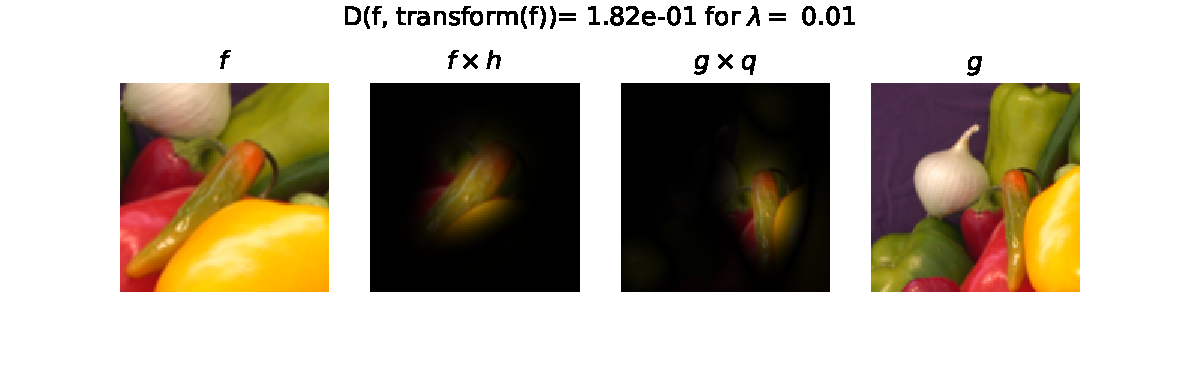
\includegraphics[width=\textwidth]{ch1-diffy/figures/fig_peppers/appendix_match_0.01_14.pdf}
%    \end{subfigure}
%    \begin{subfigure}{0.60\textwidth}
%    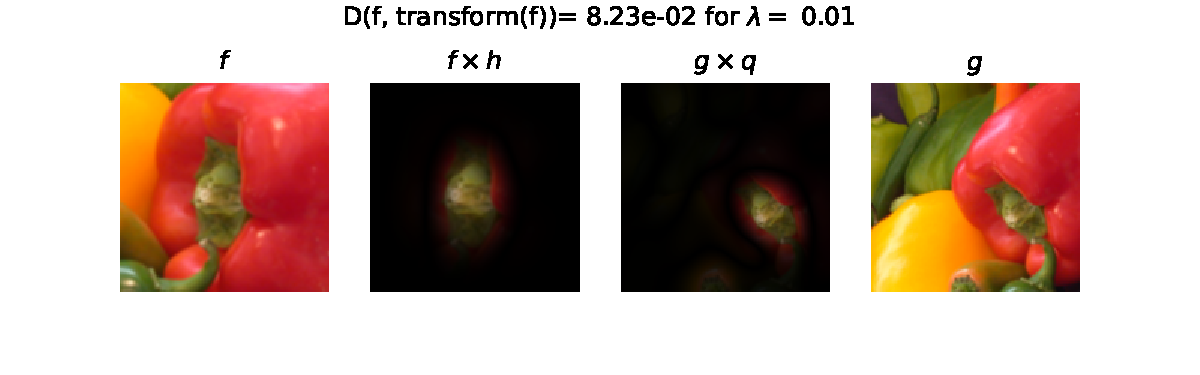
\includegraphics[width=\textwidth]{ch1-diffy/figures/fig_peppers/appendix_match_0.01_19.pdf}
%    \end{subfigure}
%    \begin{subfigure}{0.60\textwidth}
%    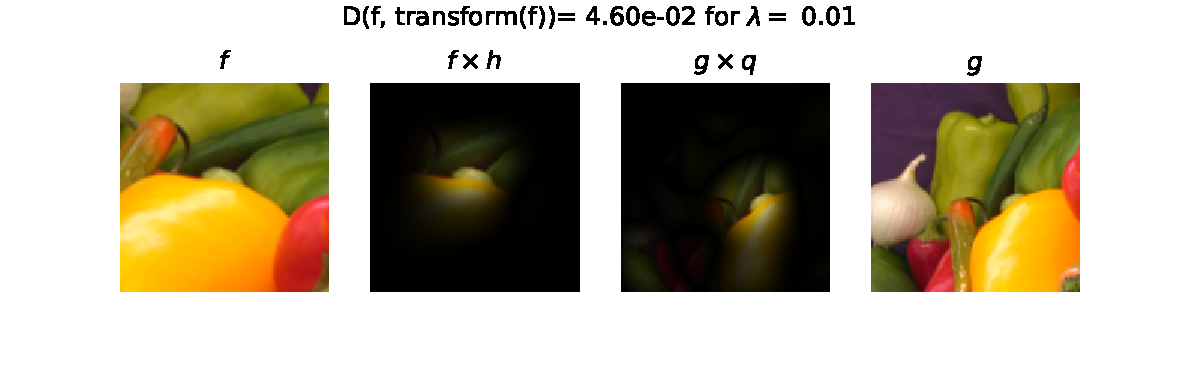
\includegraphics[width=\textwidth]{ch1-diffy/figures/fig_peppers/appendix_match_0.01_8.pdf}
%    \end{subfigure}
%    \begin{subfigure}{0.60\textwidth}
%    \includegraphics[width=\textwidth]{ch1-diffy/figures/fig_peppers/appendix_match_0.01_9.pdf}
%    \end{subfigure}
%    \begin{subfigure}{0.60\textwidth}
%    \includegraphics[width=\textwidth]{ch1-diffy/figures/fig_peppers/appendix_match_0.01_15.pdf}
%    \end{subfigure}
%    \begin{subfigure}{0.60\textwidth}
%    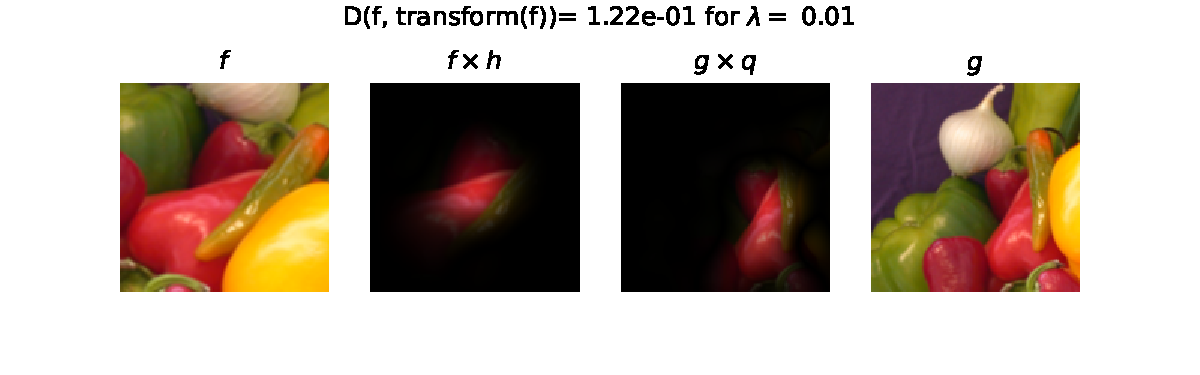
\includegraphics[width=\textwidth]{ch1-diffy/figures/fig_peppers/appendix_match_0.01_5.pdf}
%    \end{subfigure}
%    \caption{$\widehat D_\lambda(f, \textrm{transform}(f))$ for $f$ random patches from \texttt{peppers}. We show $f$, $g=\textrm{transform}(f)$ as well as the optimal functions $h$ and $q$.}
%    \label{fig:appendix-peppers-matching}
%\end{figure}


\section{Warping demonstrations}\label{sec:appendix-warping}
The warps below were generated using file \texttt{appendix\char`_warp.py} in our source code, using an image from ImageNet. Rows are from different samples, columns for different warp temperatures. All waps use $c=2$.

%todo : hidden for compilation speed
%\begin{figure}[!h]
%    \centering
%    \begin{subfigure}{0.18\textwidth}
%    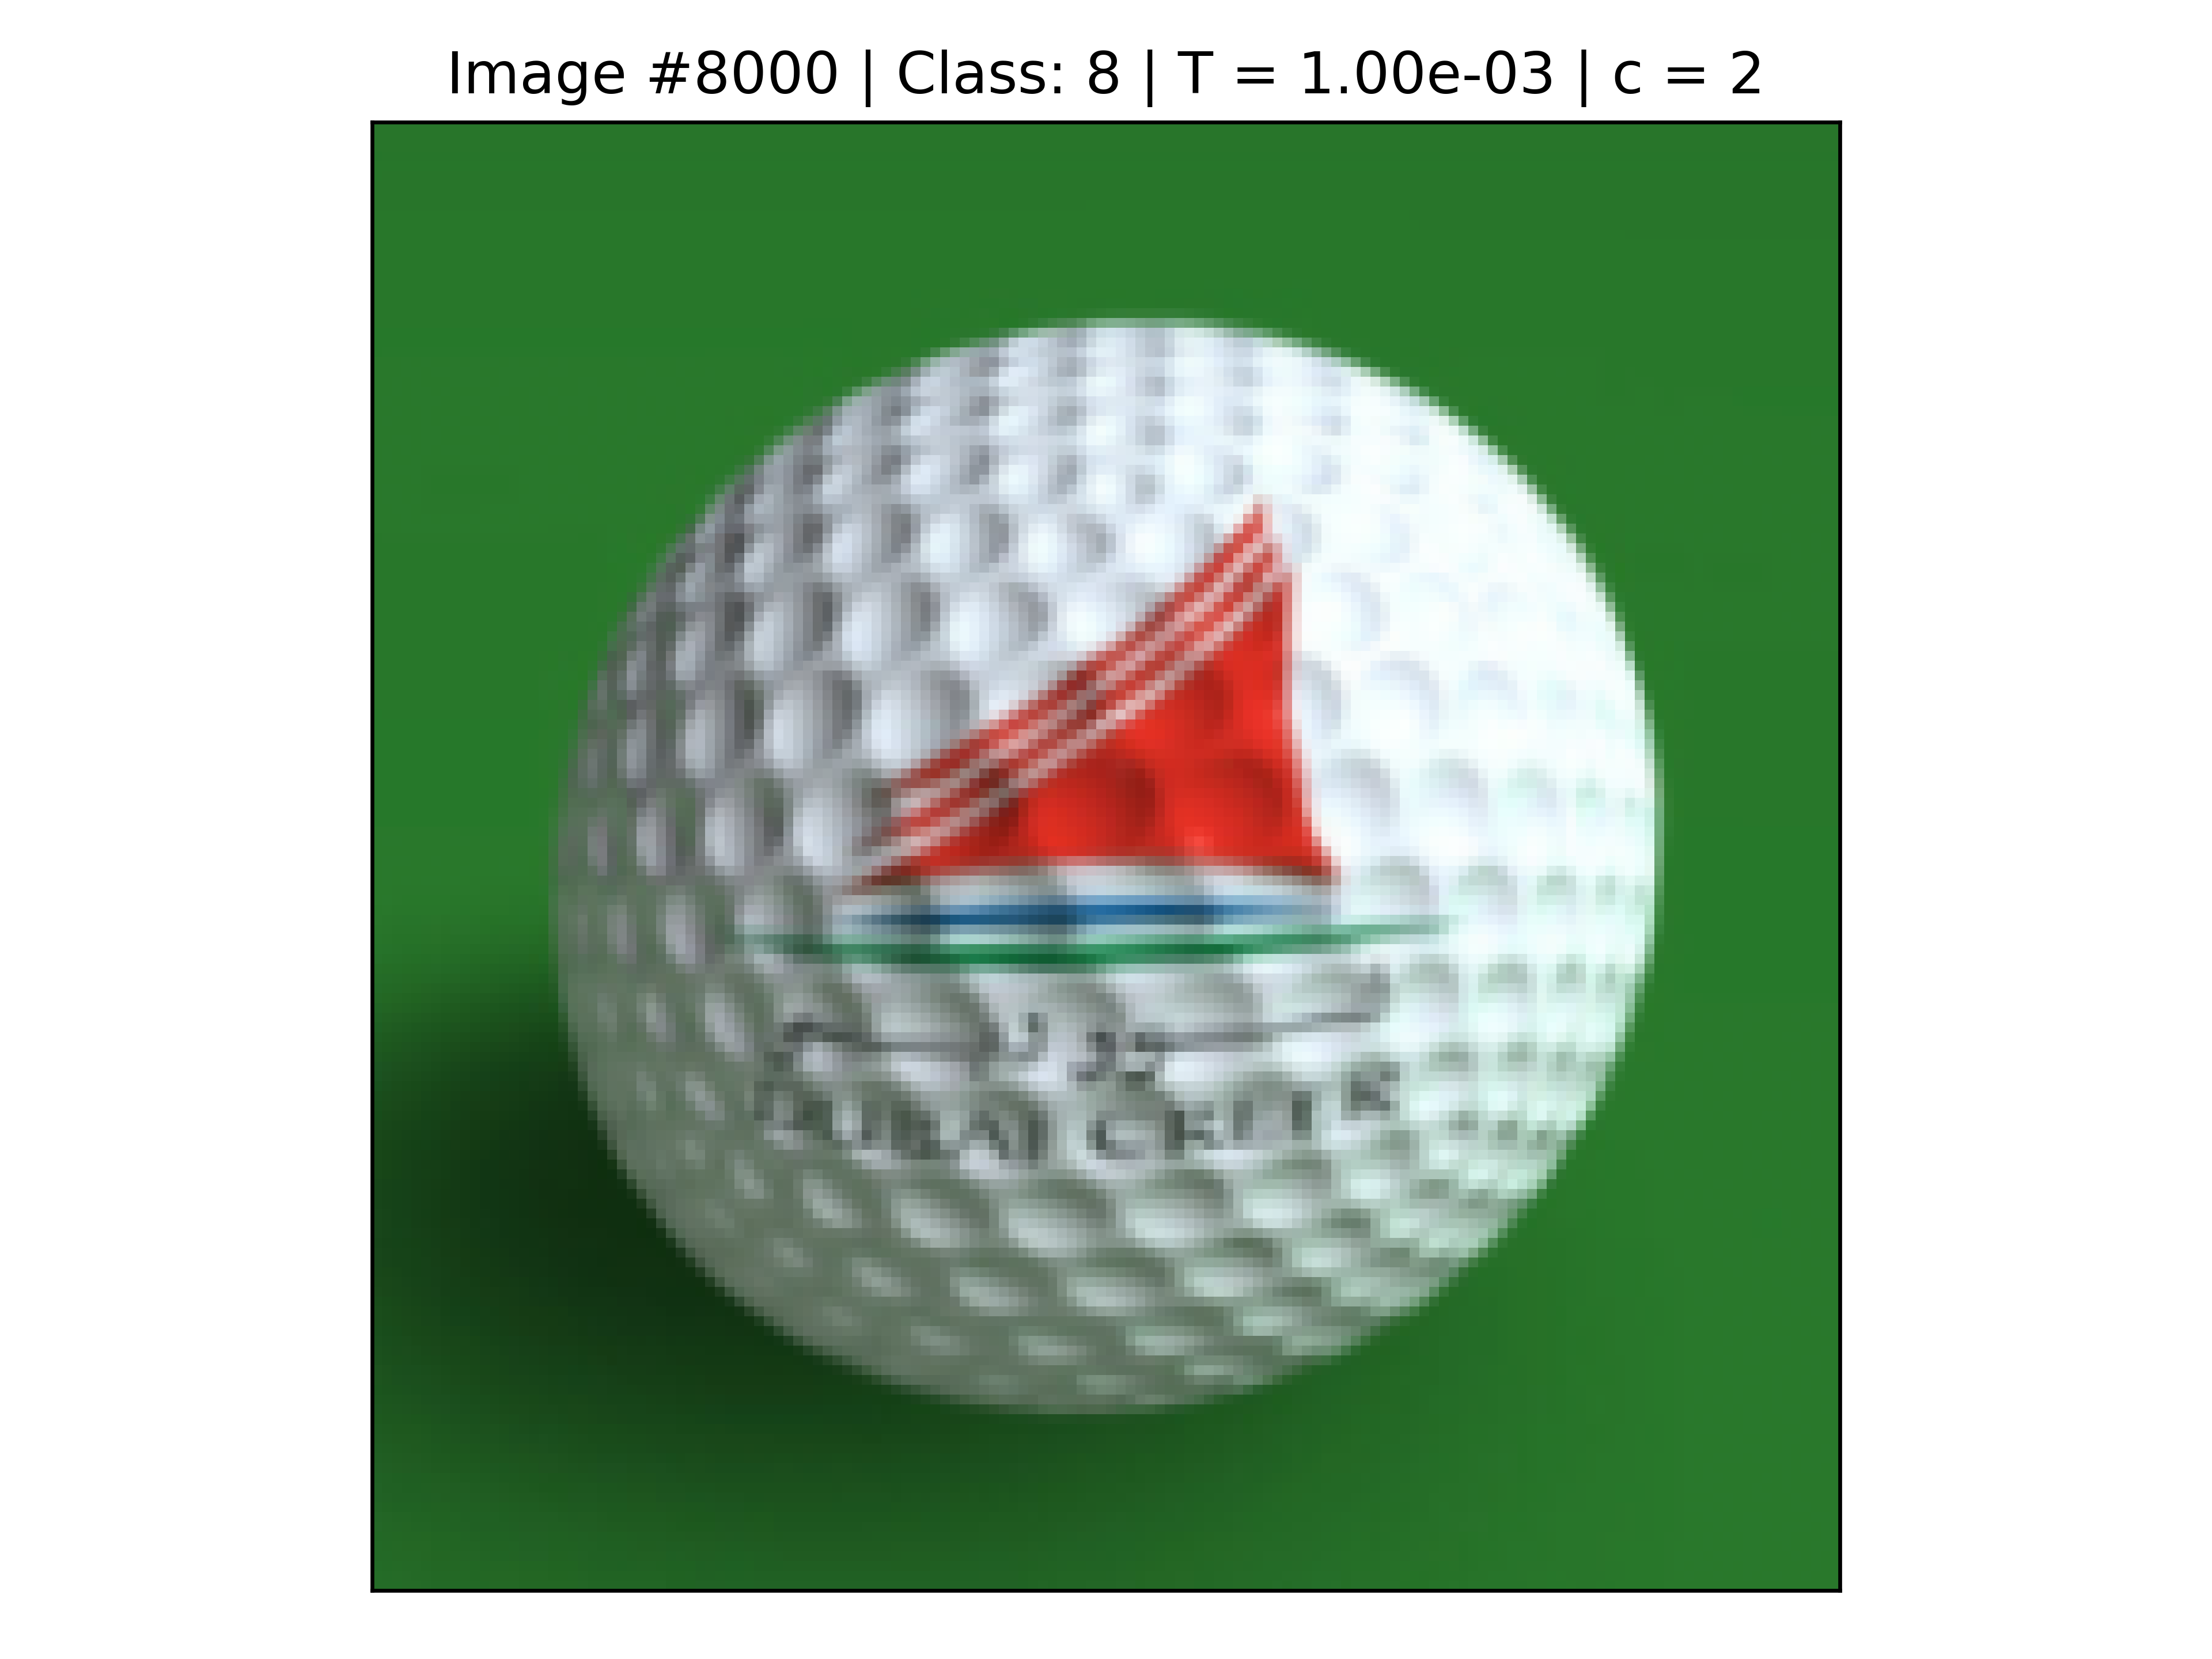
\includegraphics[width=\textwidth]{ch1-diffy/figures/warping_examples/8000_3_0.png}
%    \caption{$T=10^{-3}$}
%    % \label{fig:my_label}
%    \end{subfigure}
%    \begin{subfigure}{0.18\textwidth}
%    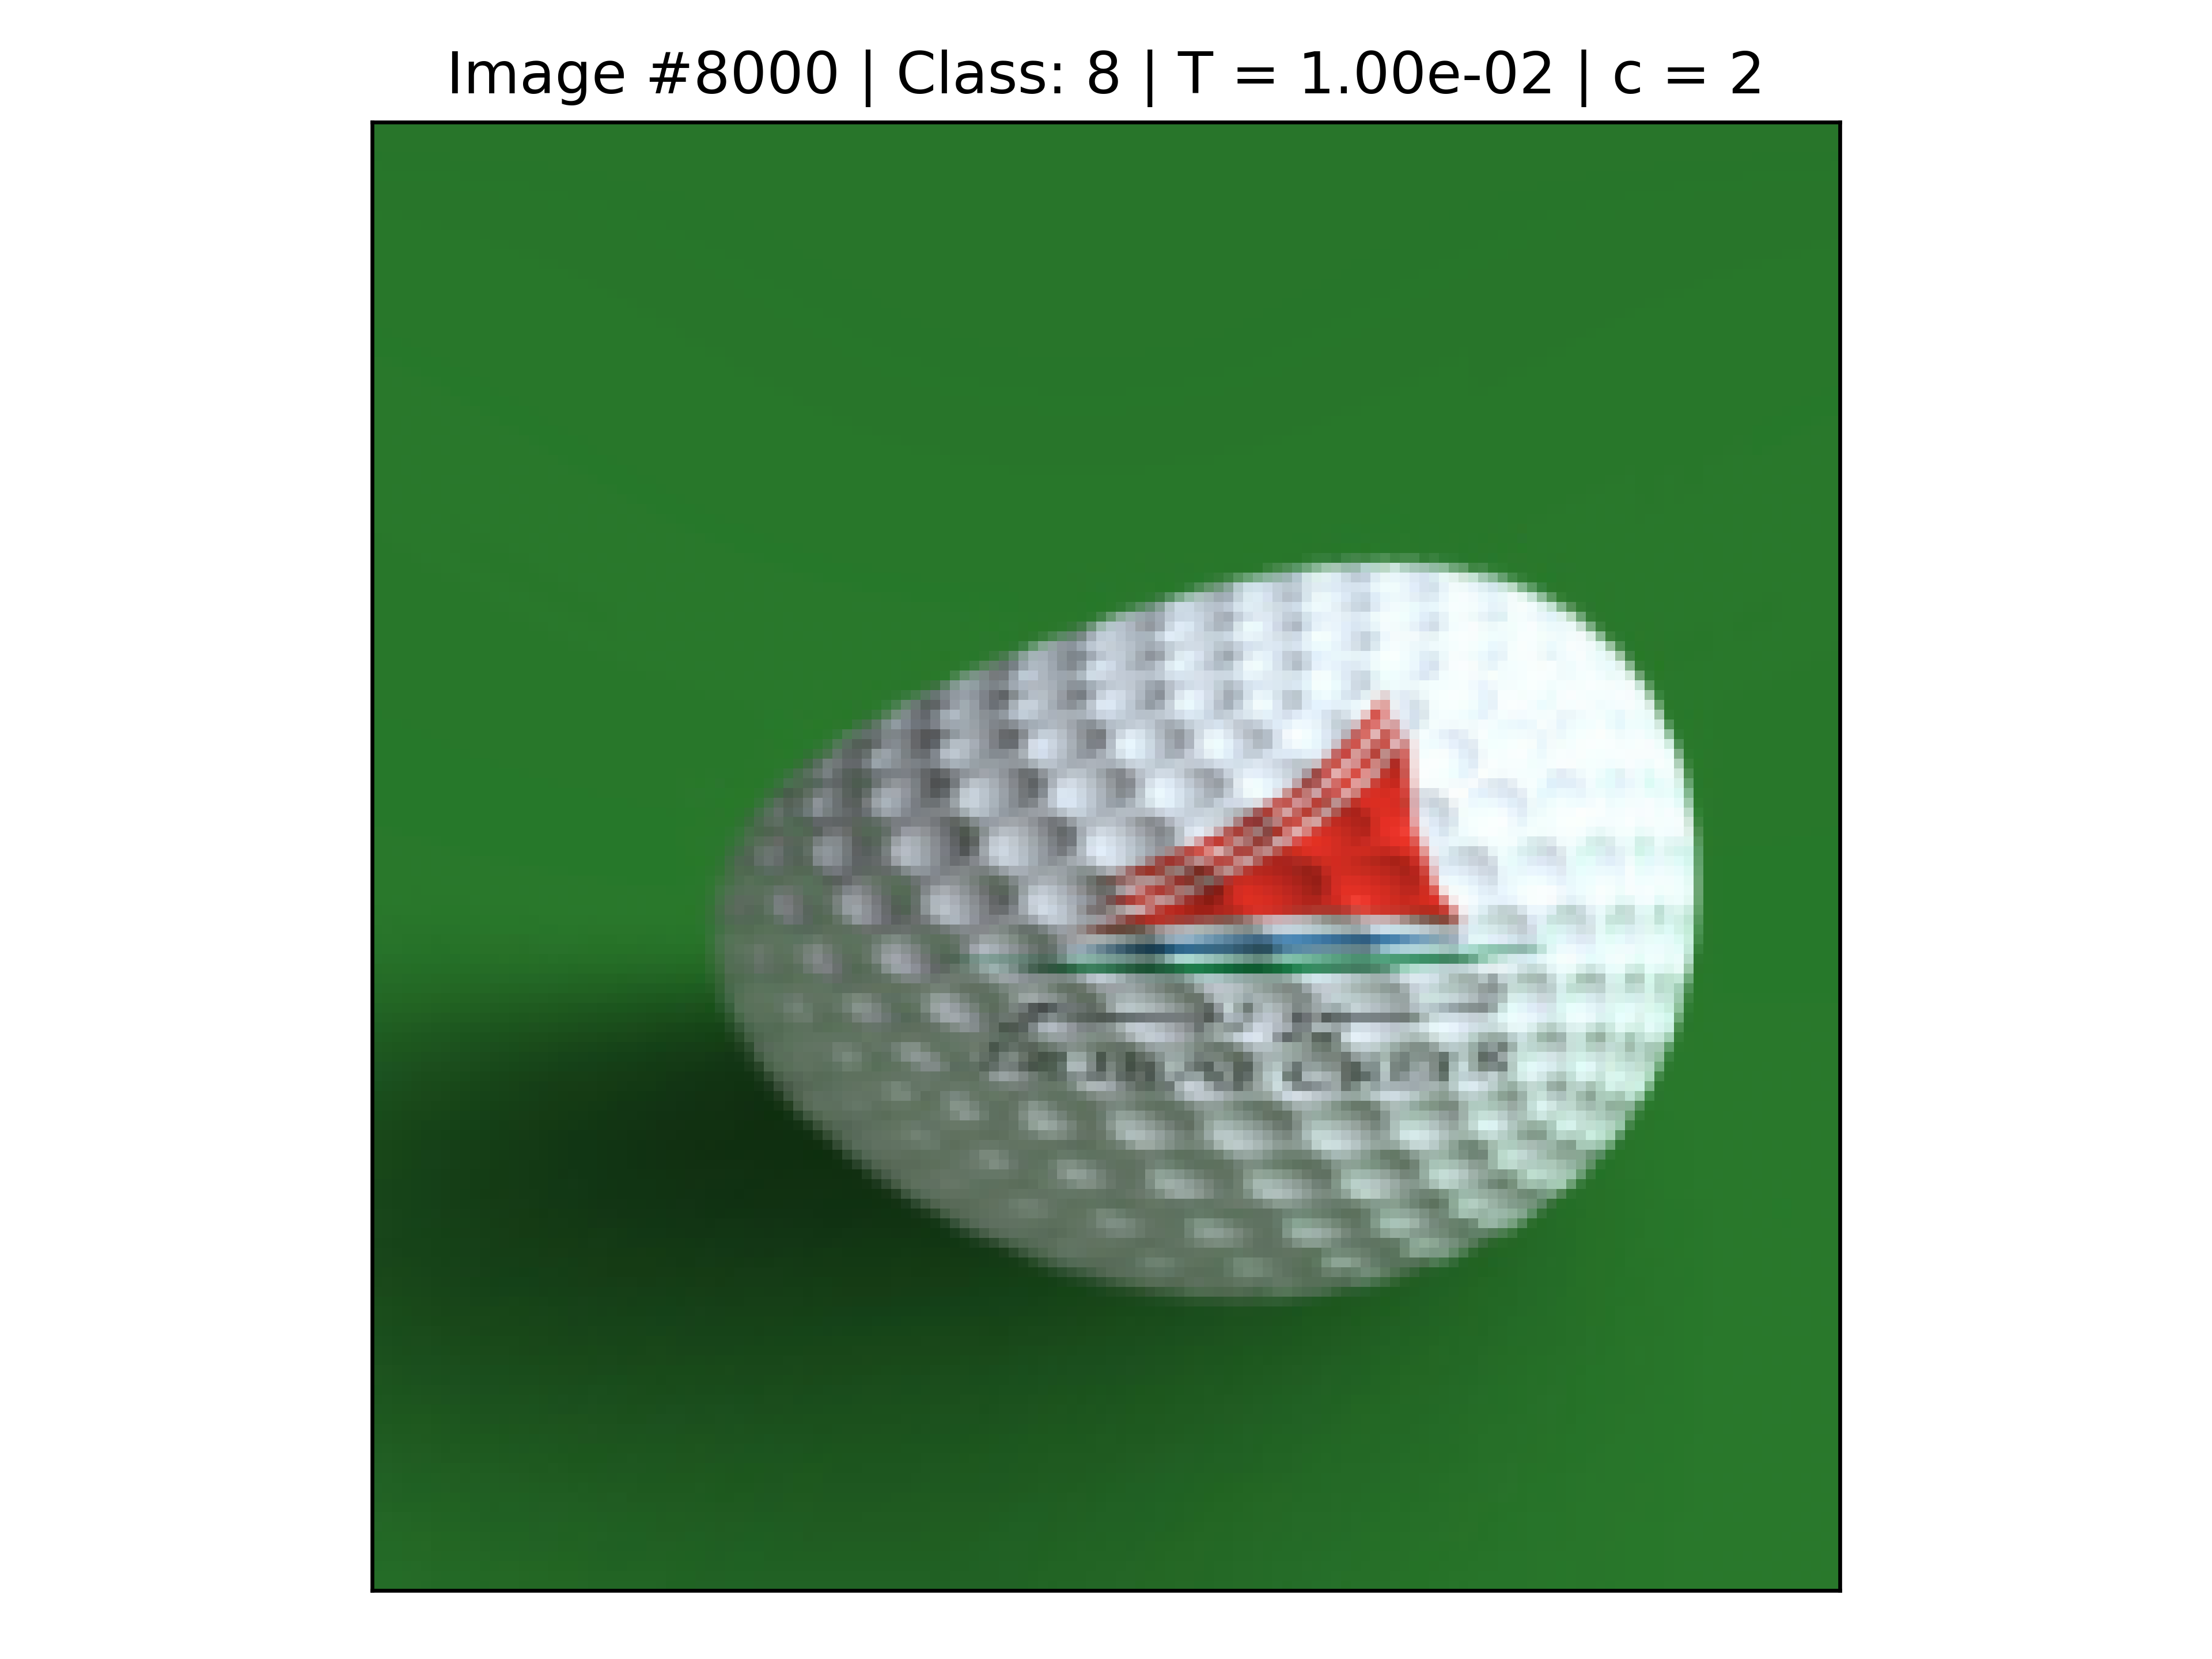
\includegraphics[width=\textwidth]{ch1-diffy/figures/warping_examples/8000_2_0.png}
%    \caption{$T=10^{-2}$}
%    % \label{fig:my_label}
%    \end{subfigure}
%    \begin{subfigure}{0.18\textwidth}
%    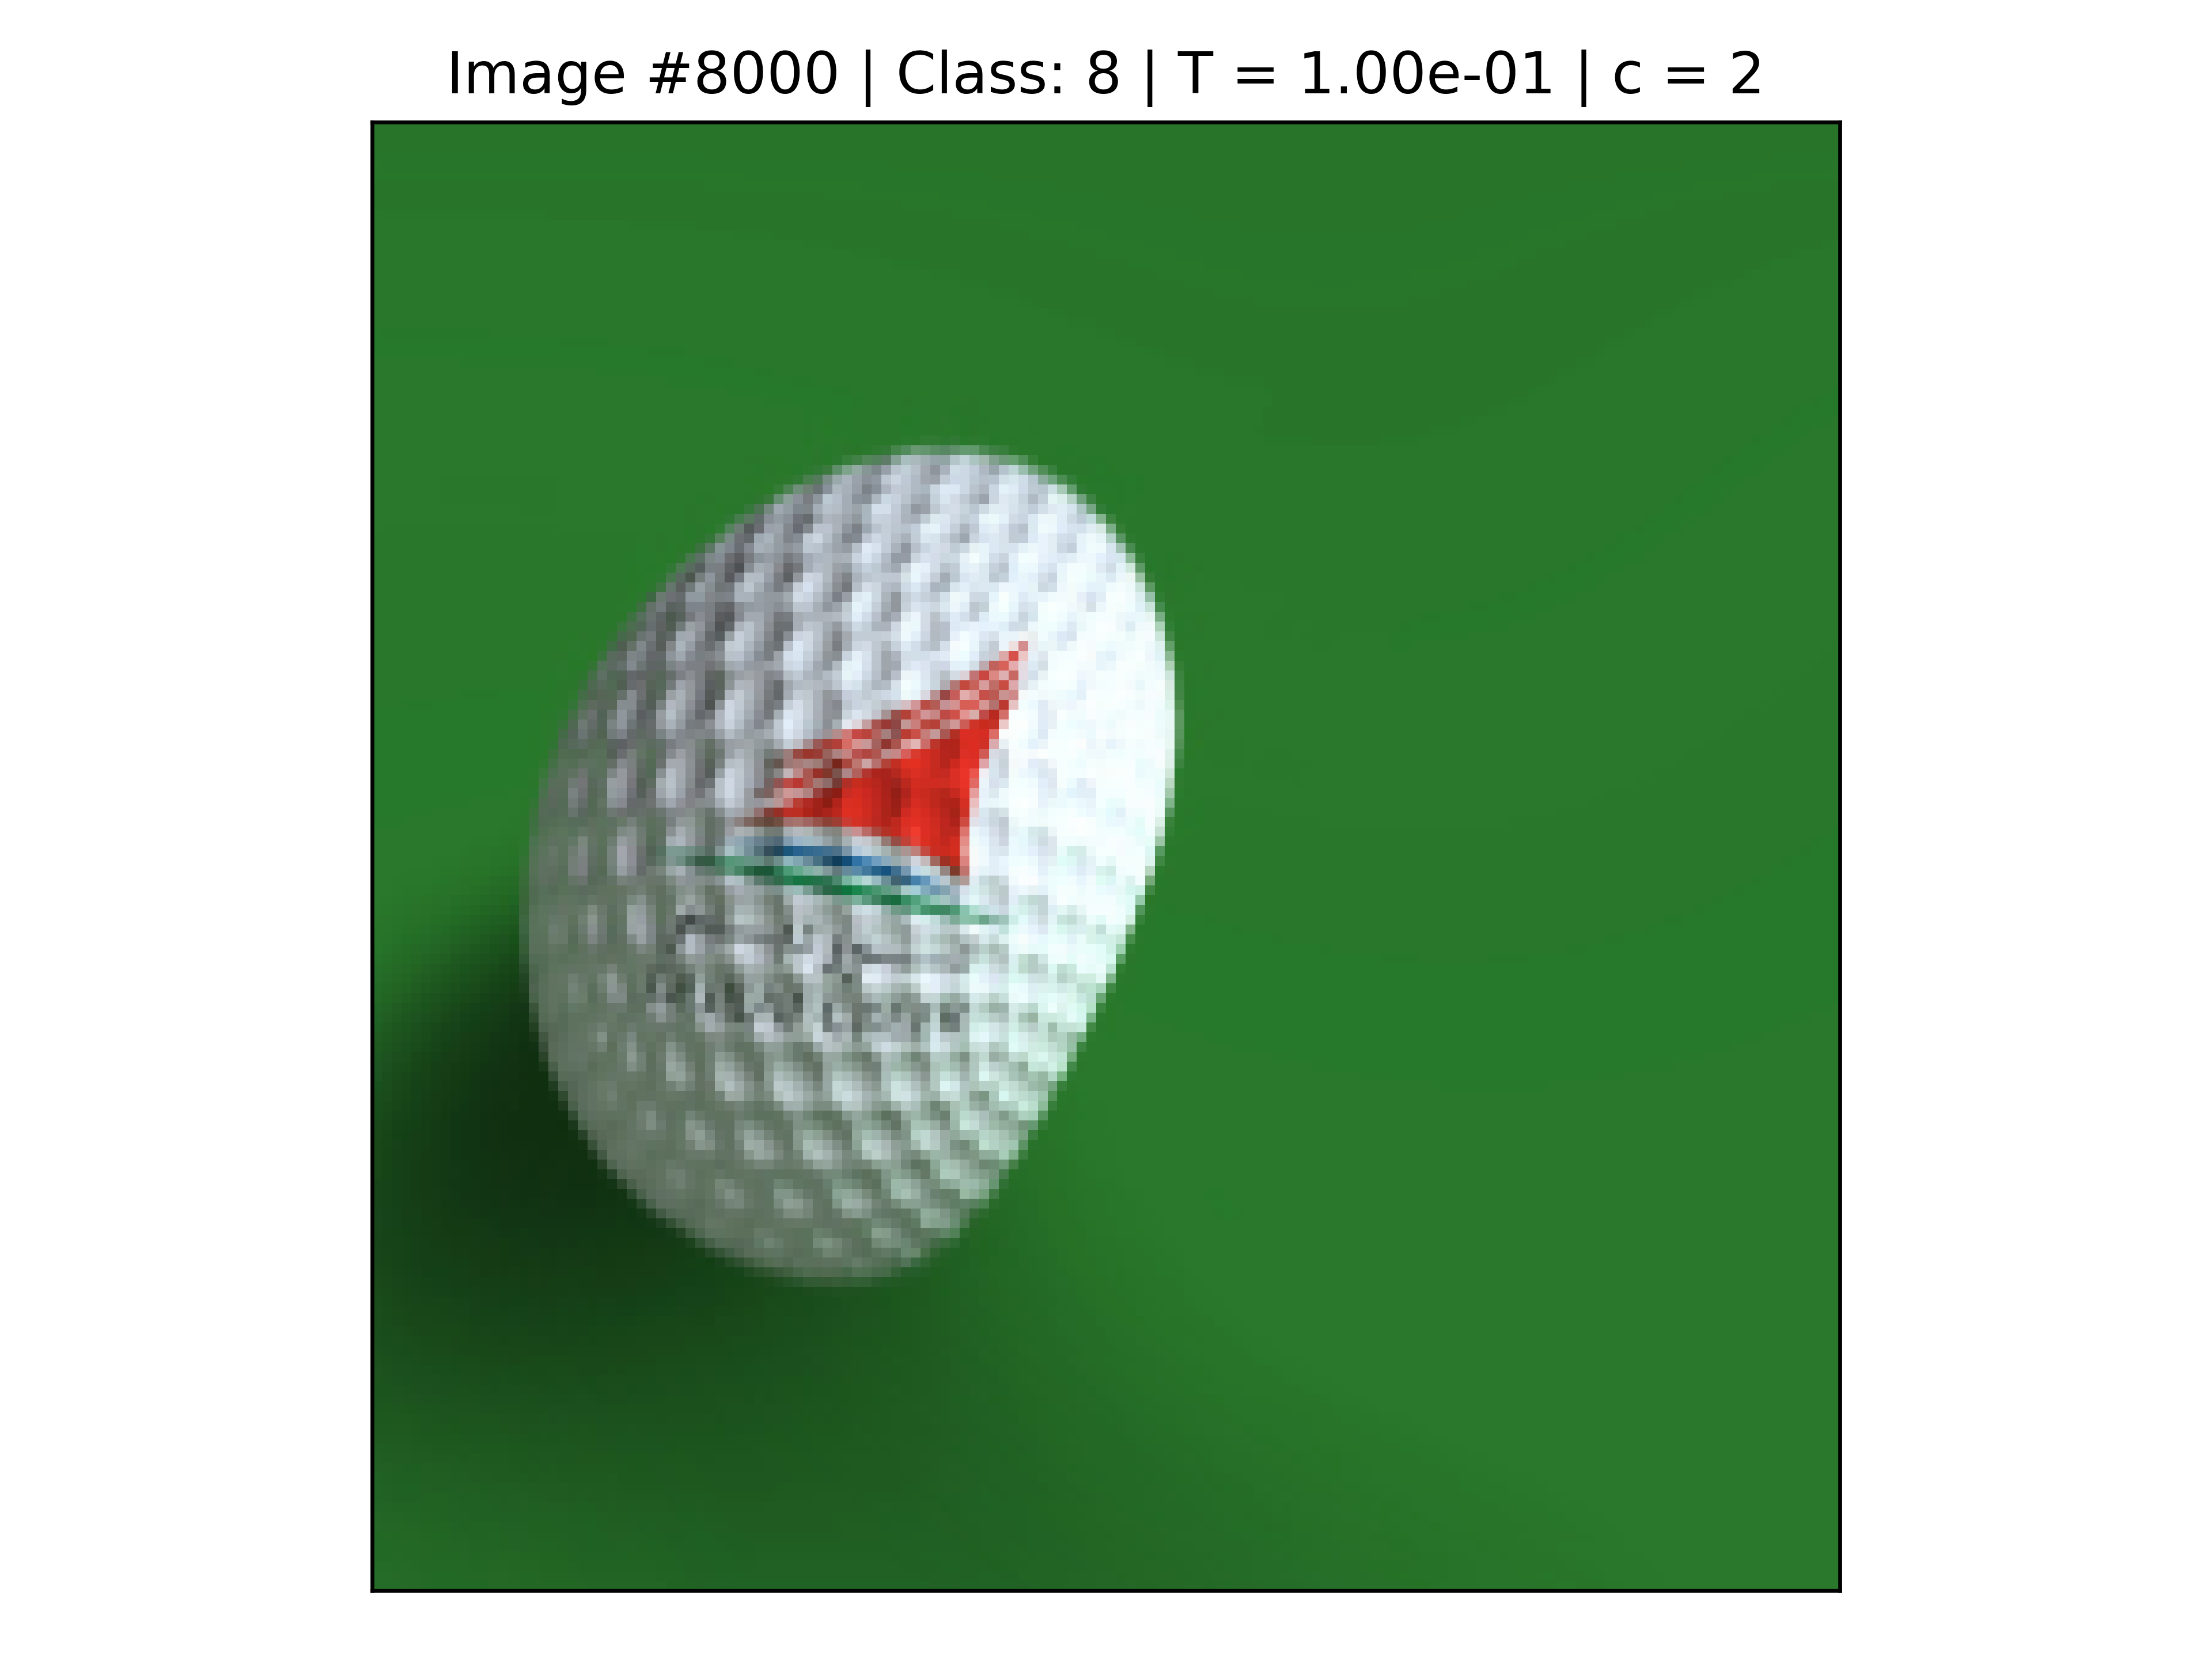
\includegraphics[width=\textwidth]{ch1-diffy/figures/warping_examples/8000_1_0.png}
%    \caption{$T=10^{-1}$}
%    % \label{fig:my_label}
%    \end{subfigure}
%    \begin{subfigure}{0.18\textwidth}
%    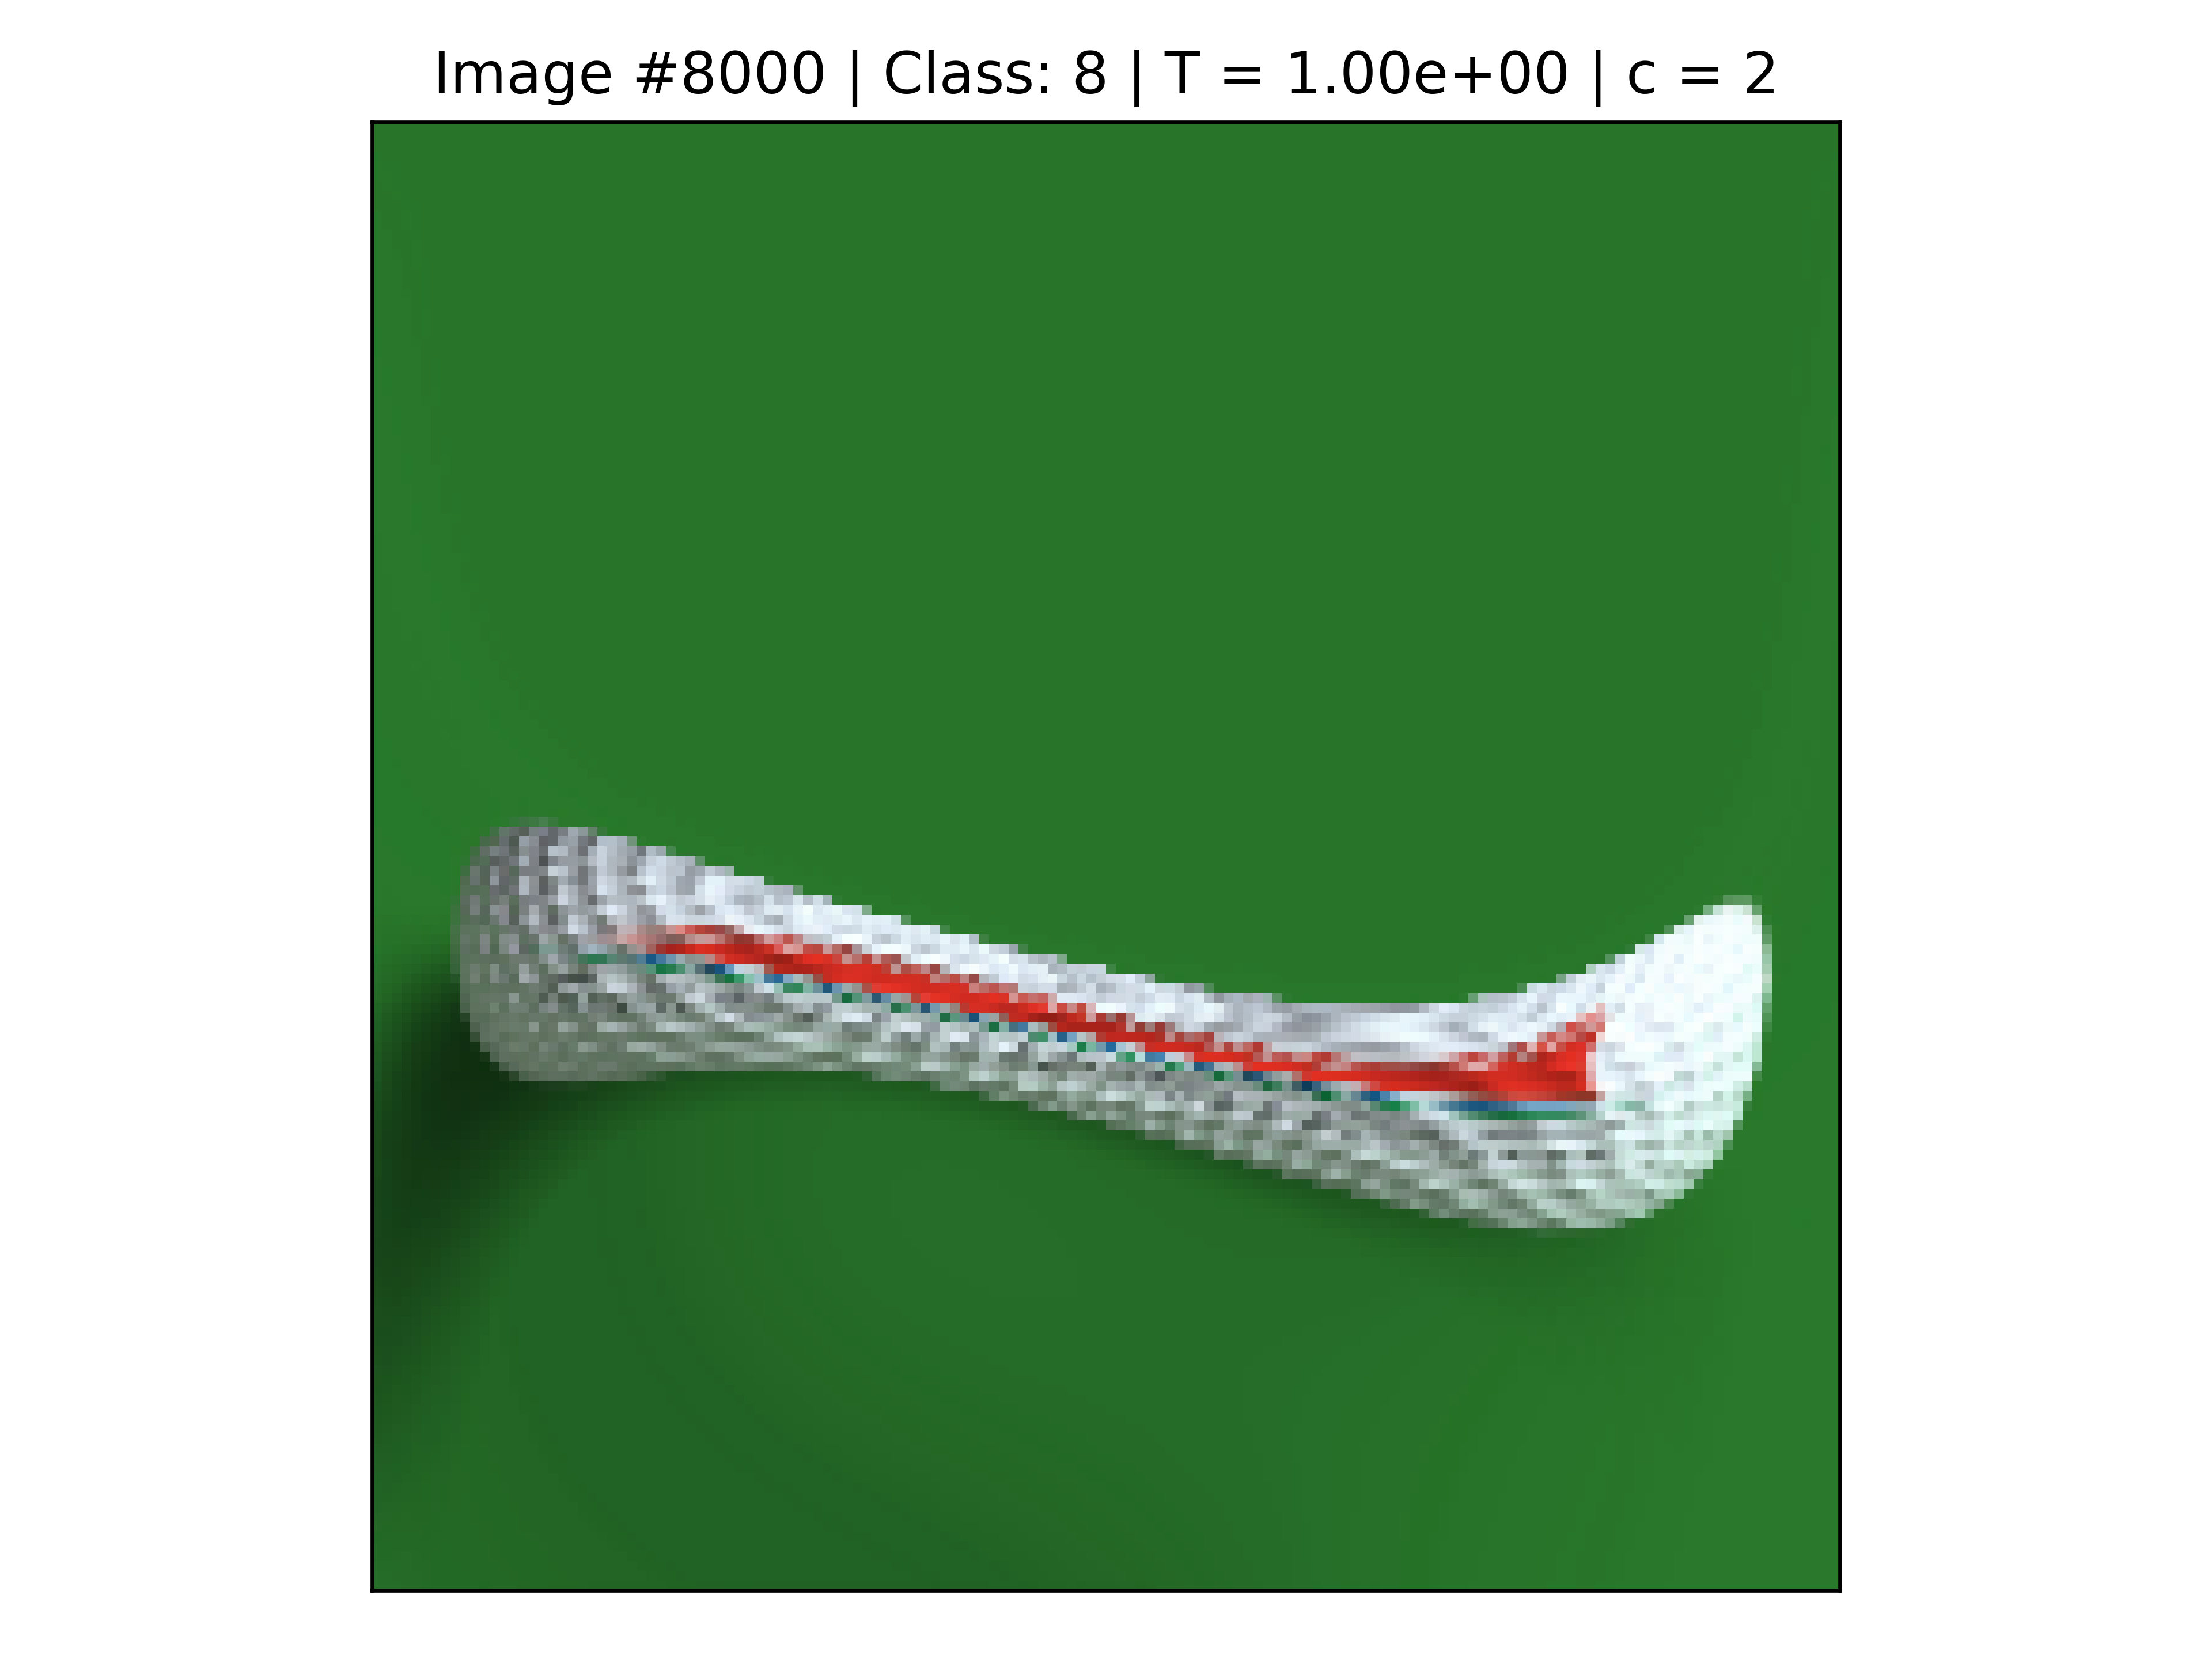
\includegraphics[width=\textwidth]{ch1-diffy/figures/warping_examples/8000_0_0.png}
%    \caption{$T=1$}
%    % \label{fig:my_label}
%    \end{subfigure}
%    \begin{subfigure}{0.18\textwidth}
%    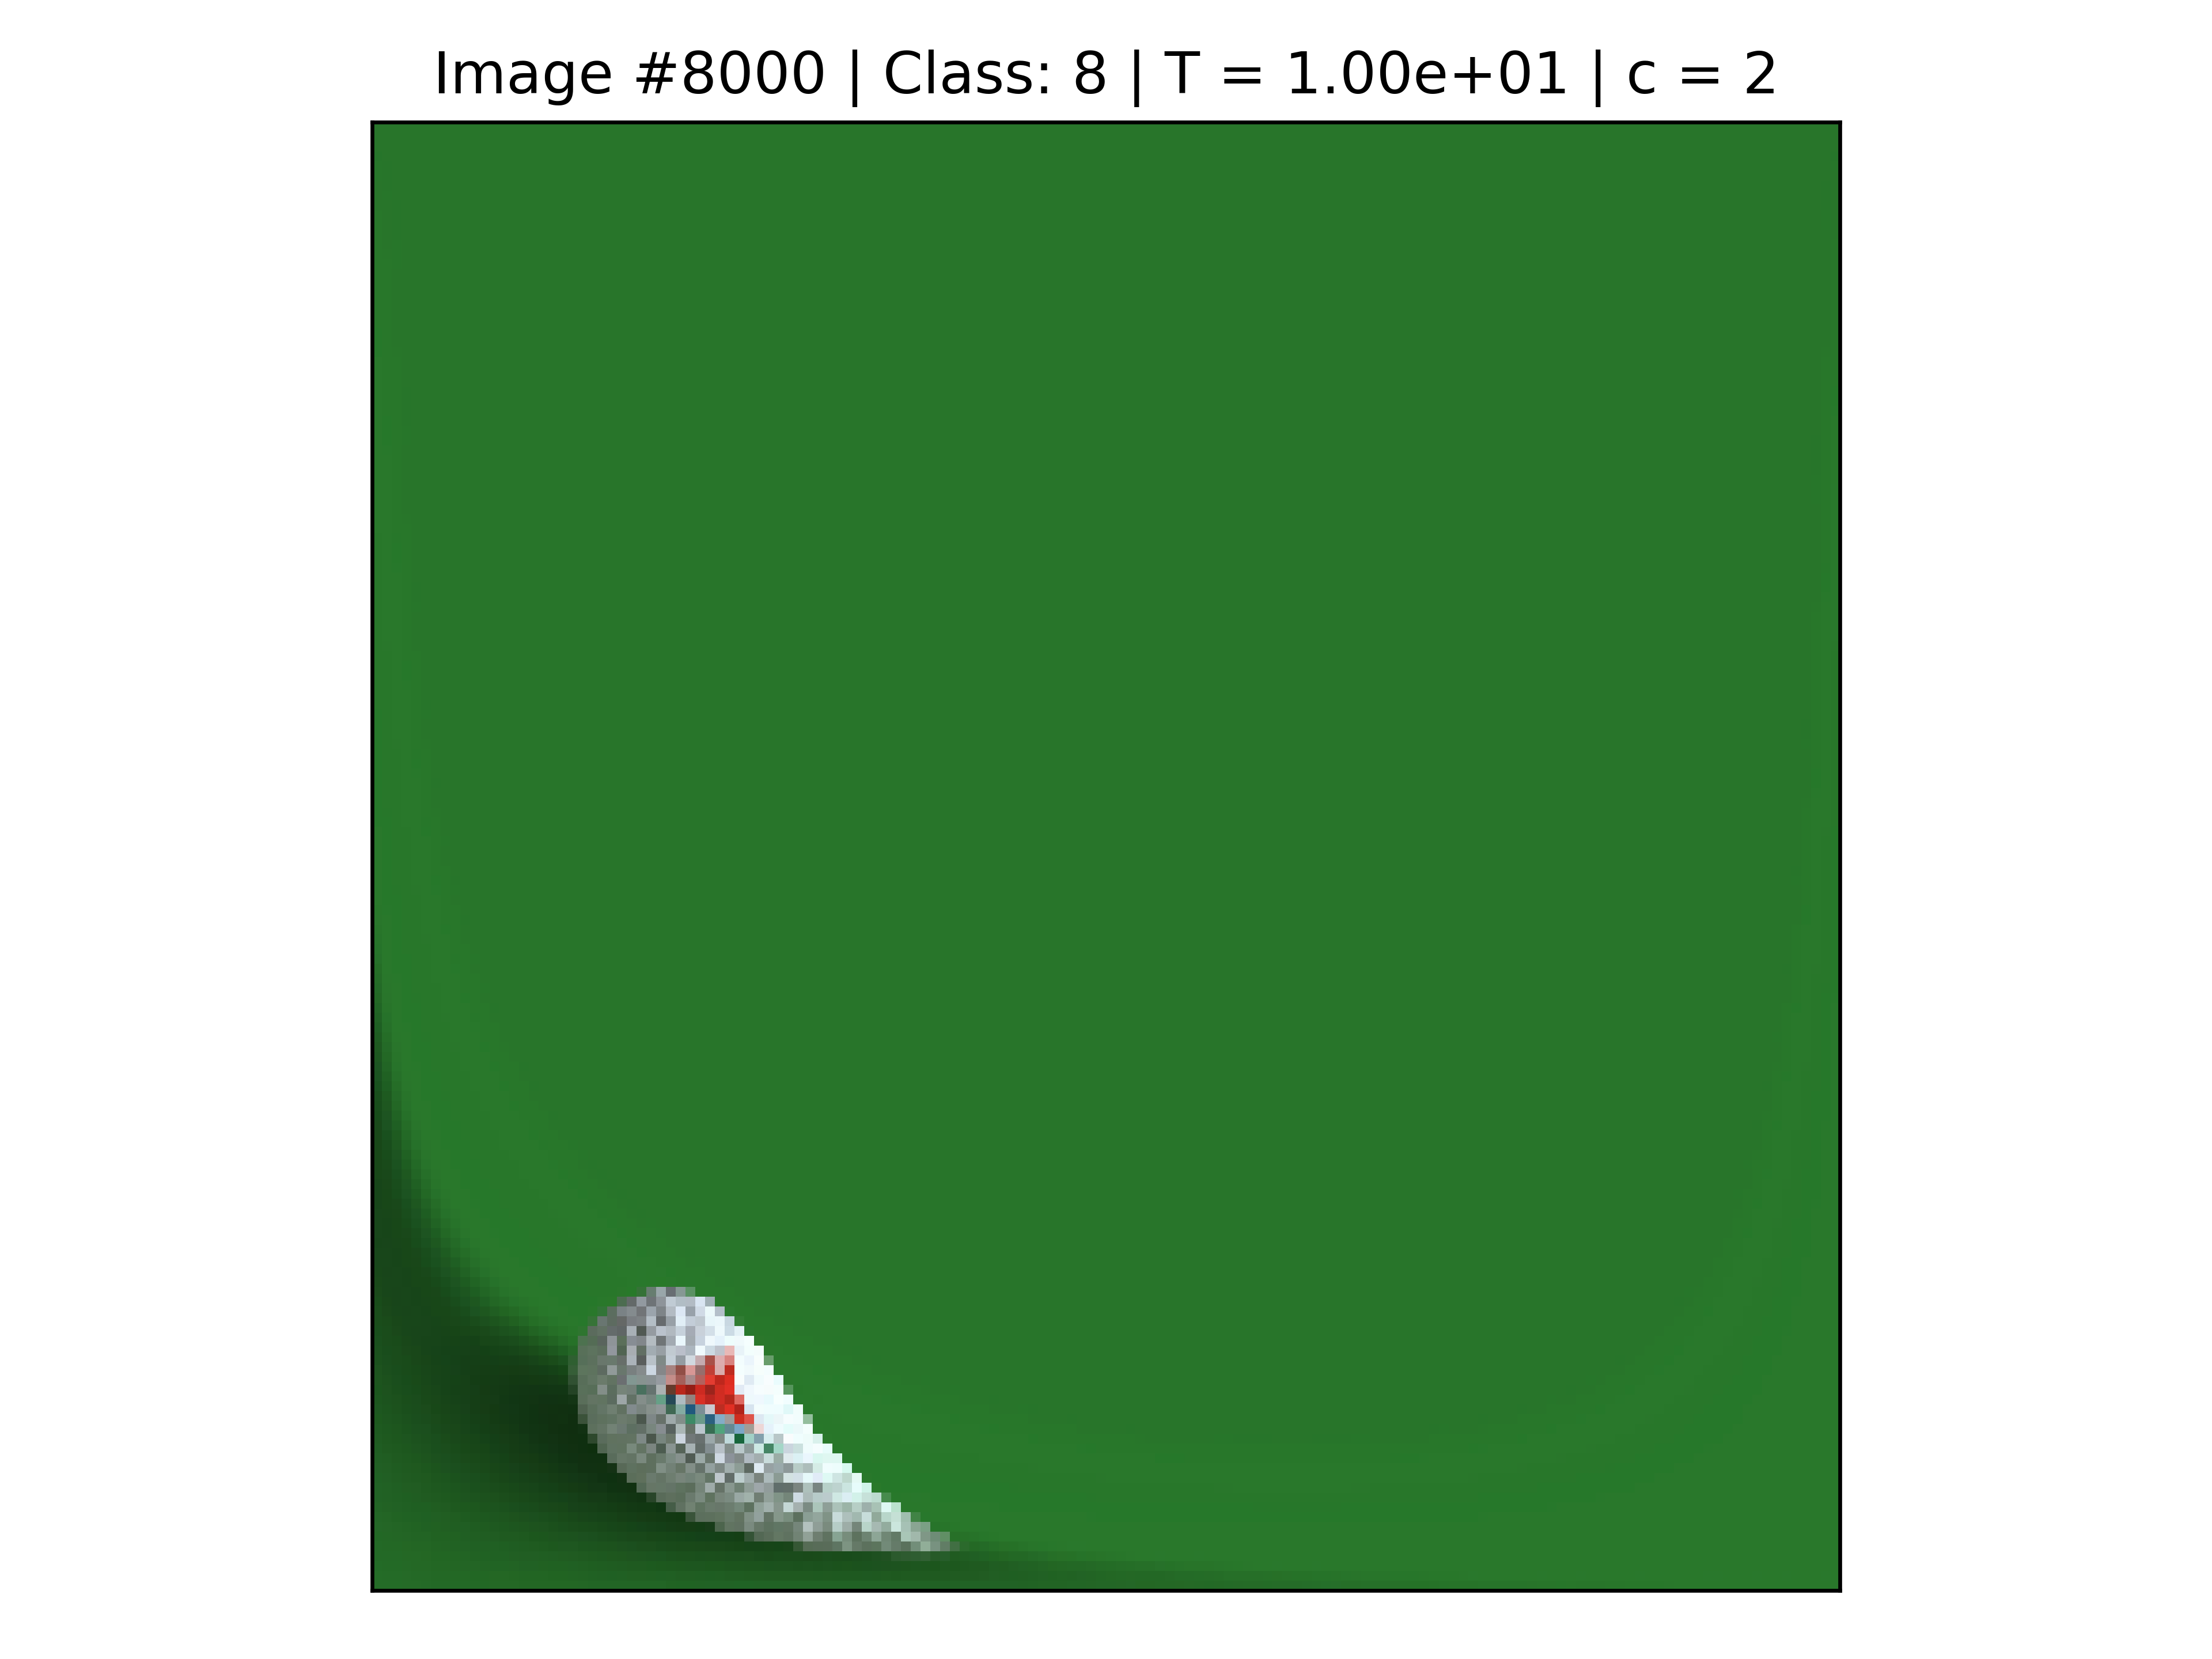
\includegraphics[width=\textwidth]{ch1-diffy/figures/warping_examples/8000_-1_0.png}
%    \caption{$T=10$}
%    % \label{fig:my_label}
%    \end{subfigure}
%    %%%%%
%    \begin{subfigure}{0.18\textwidth}
%    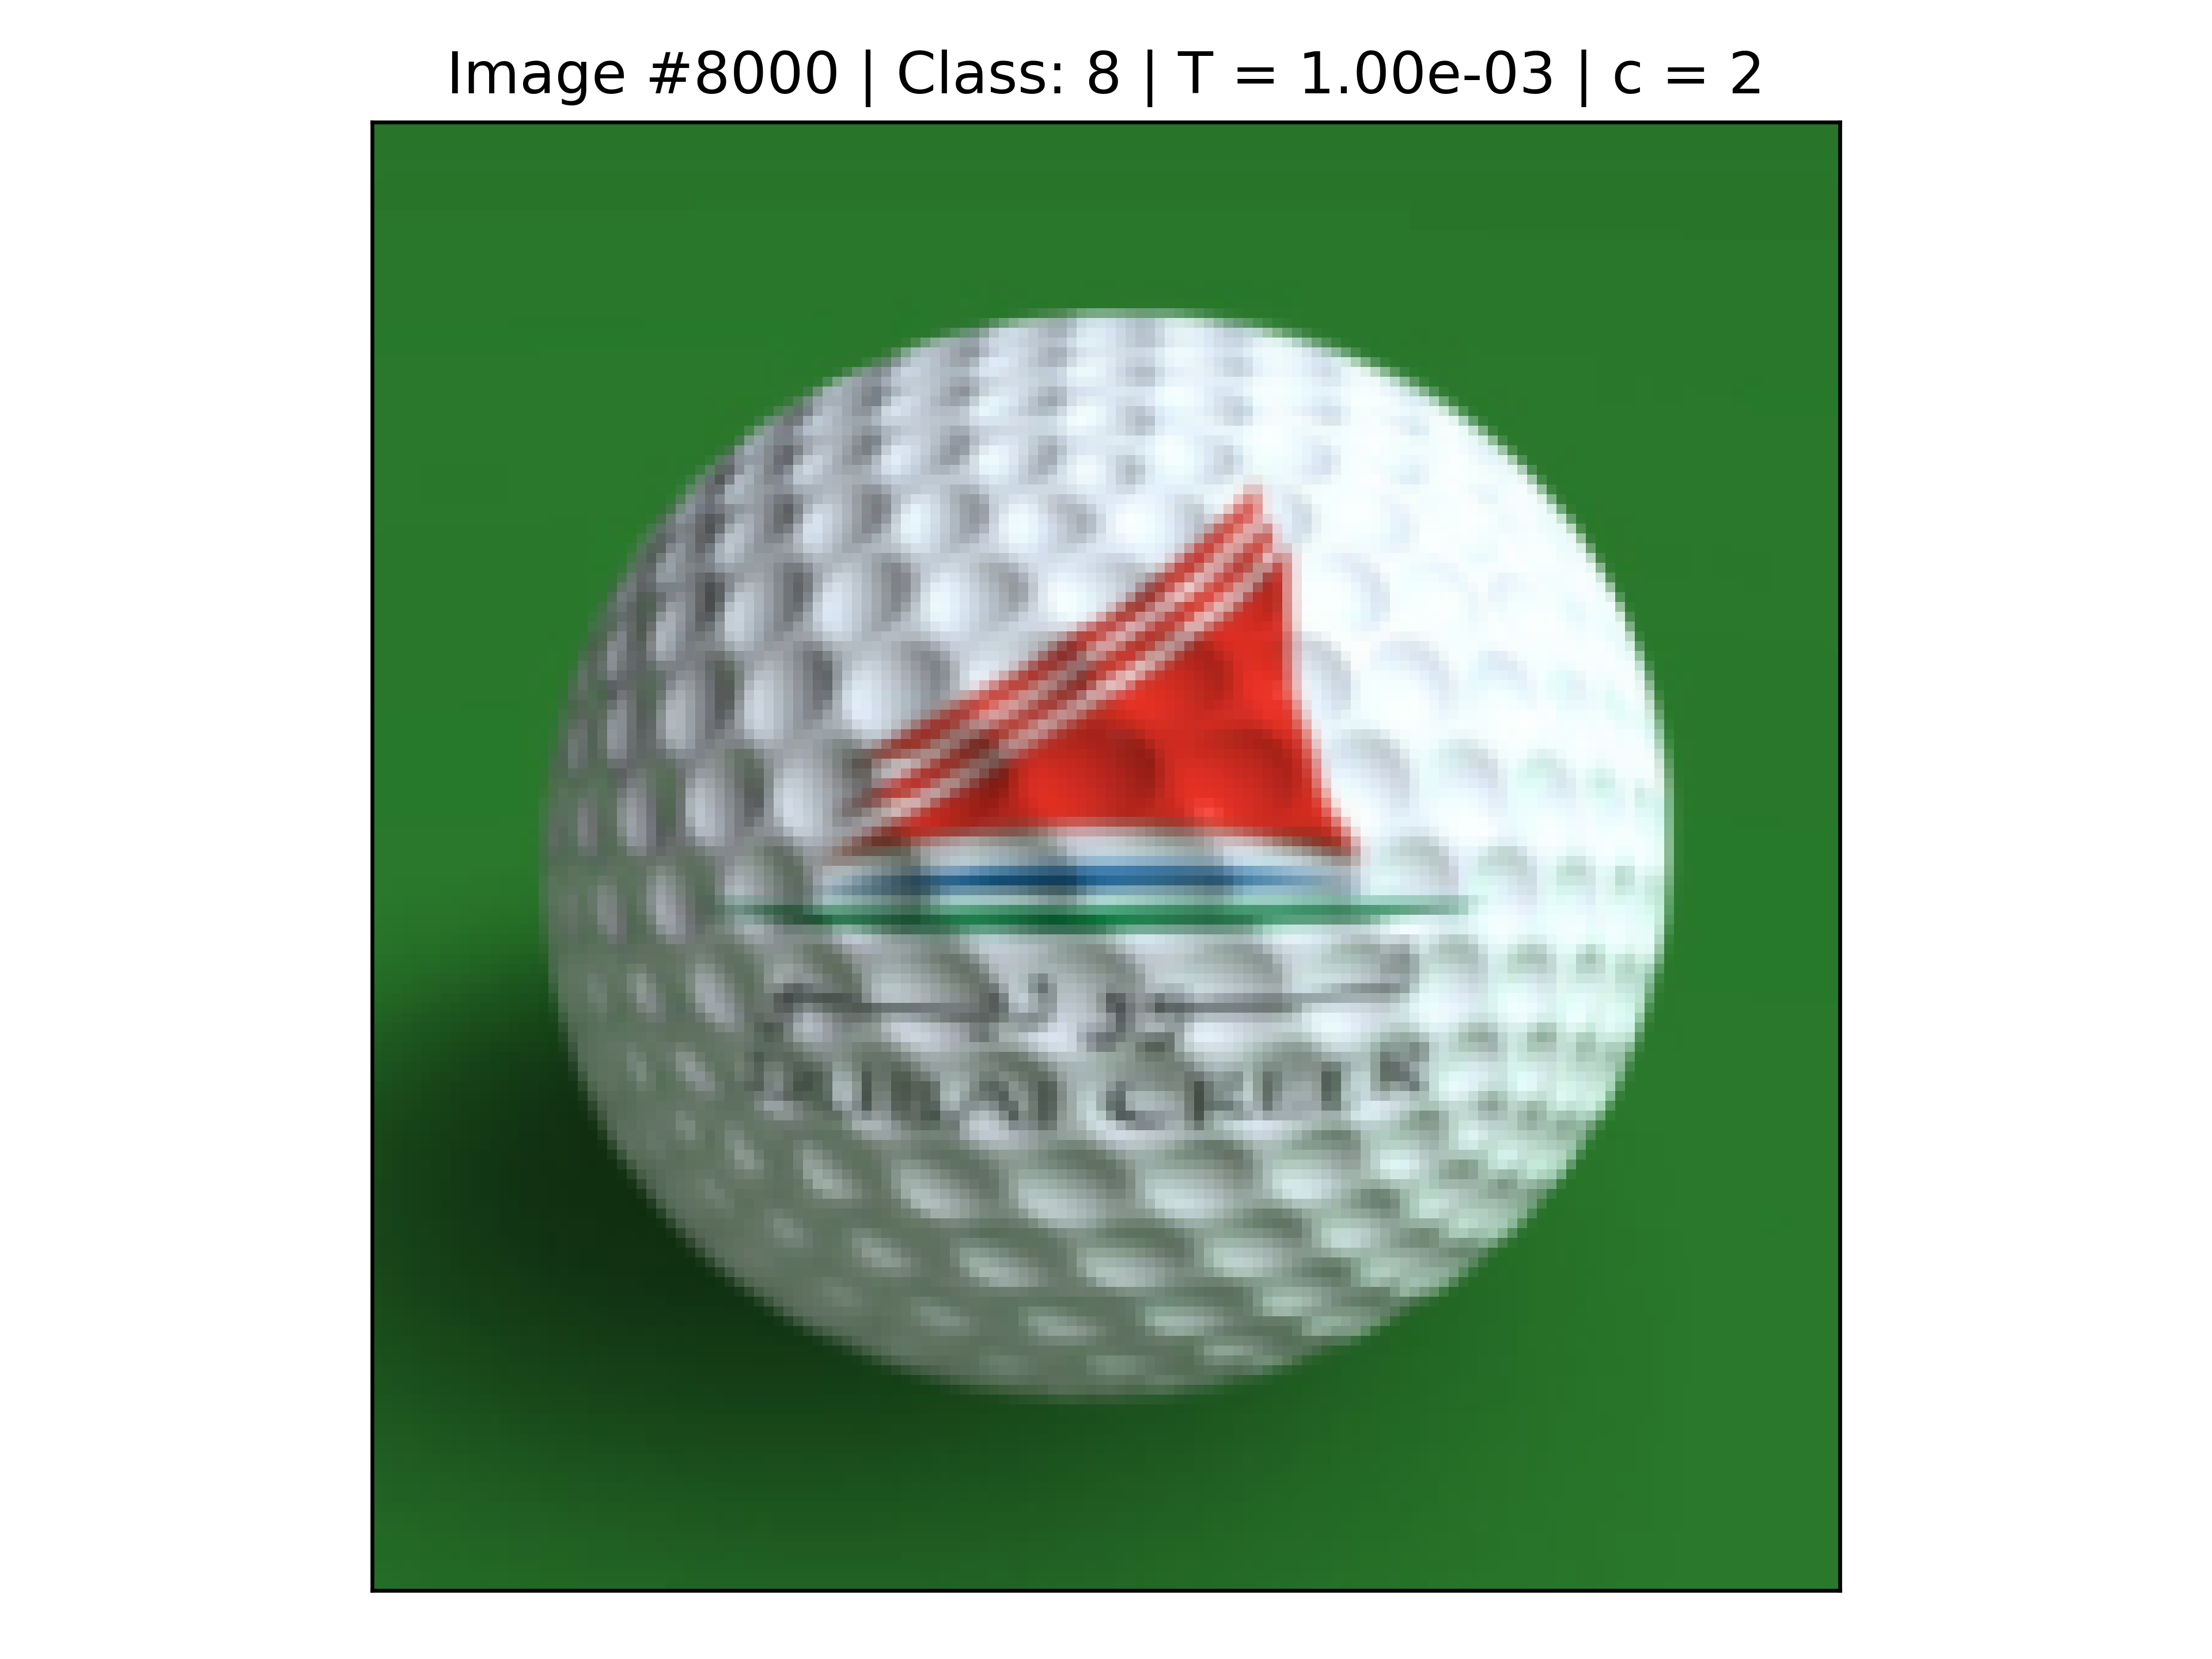
\includegraphics[width=\textwidth]{ch1-diffy/figures/warping_examples/8000_3_1.png}
%    \caption{$T=10^{-3}$}
%    % \label{fig:my_label}
%    \end{subfigure}
%    \begin{subfigure}{0.18\textwidth}
%    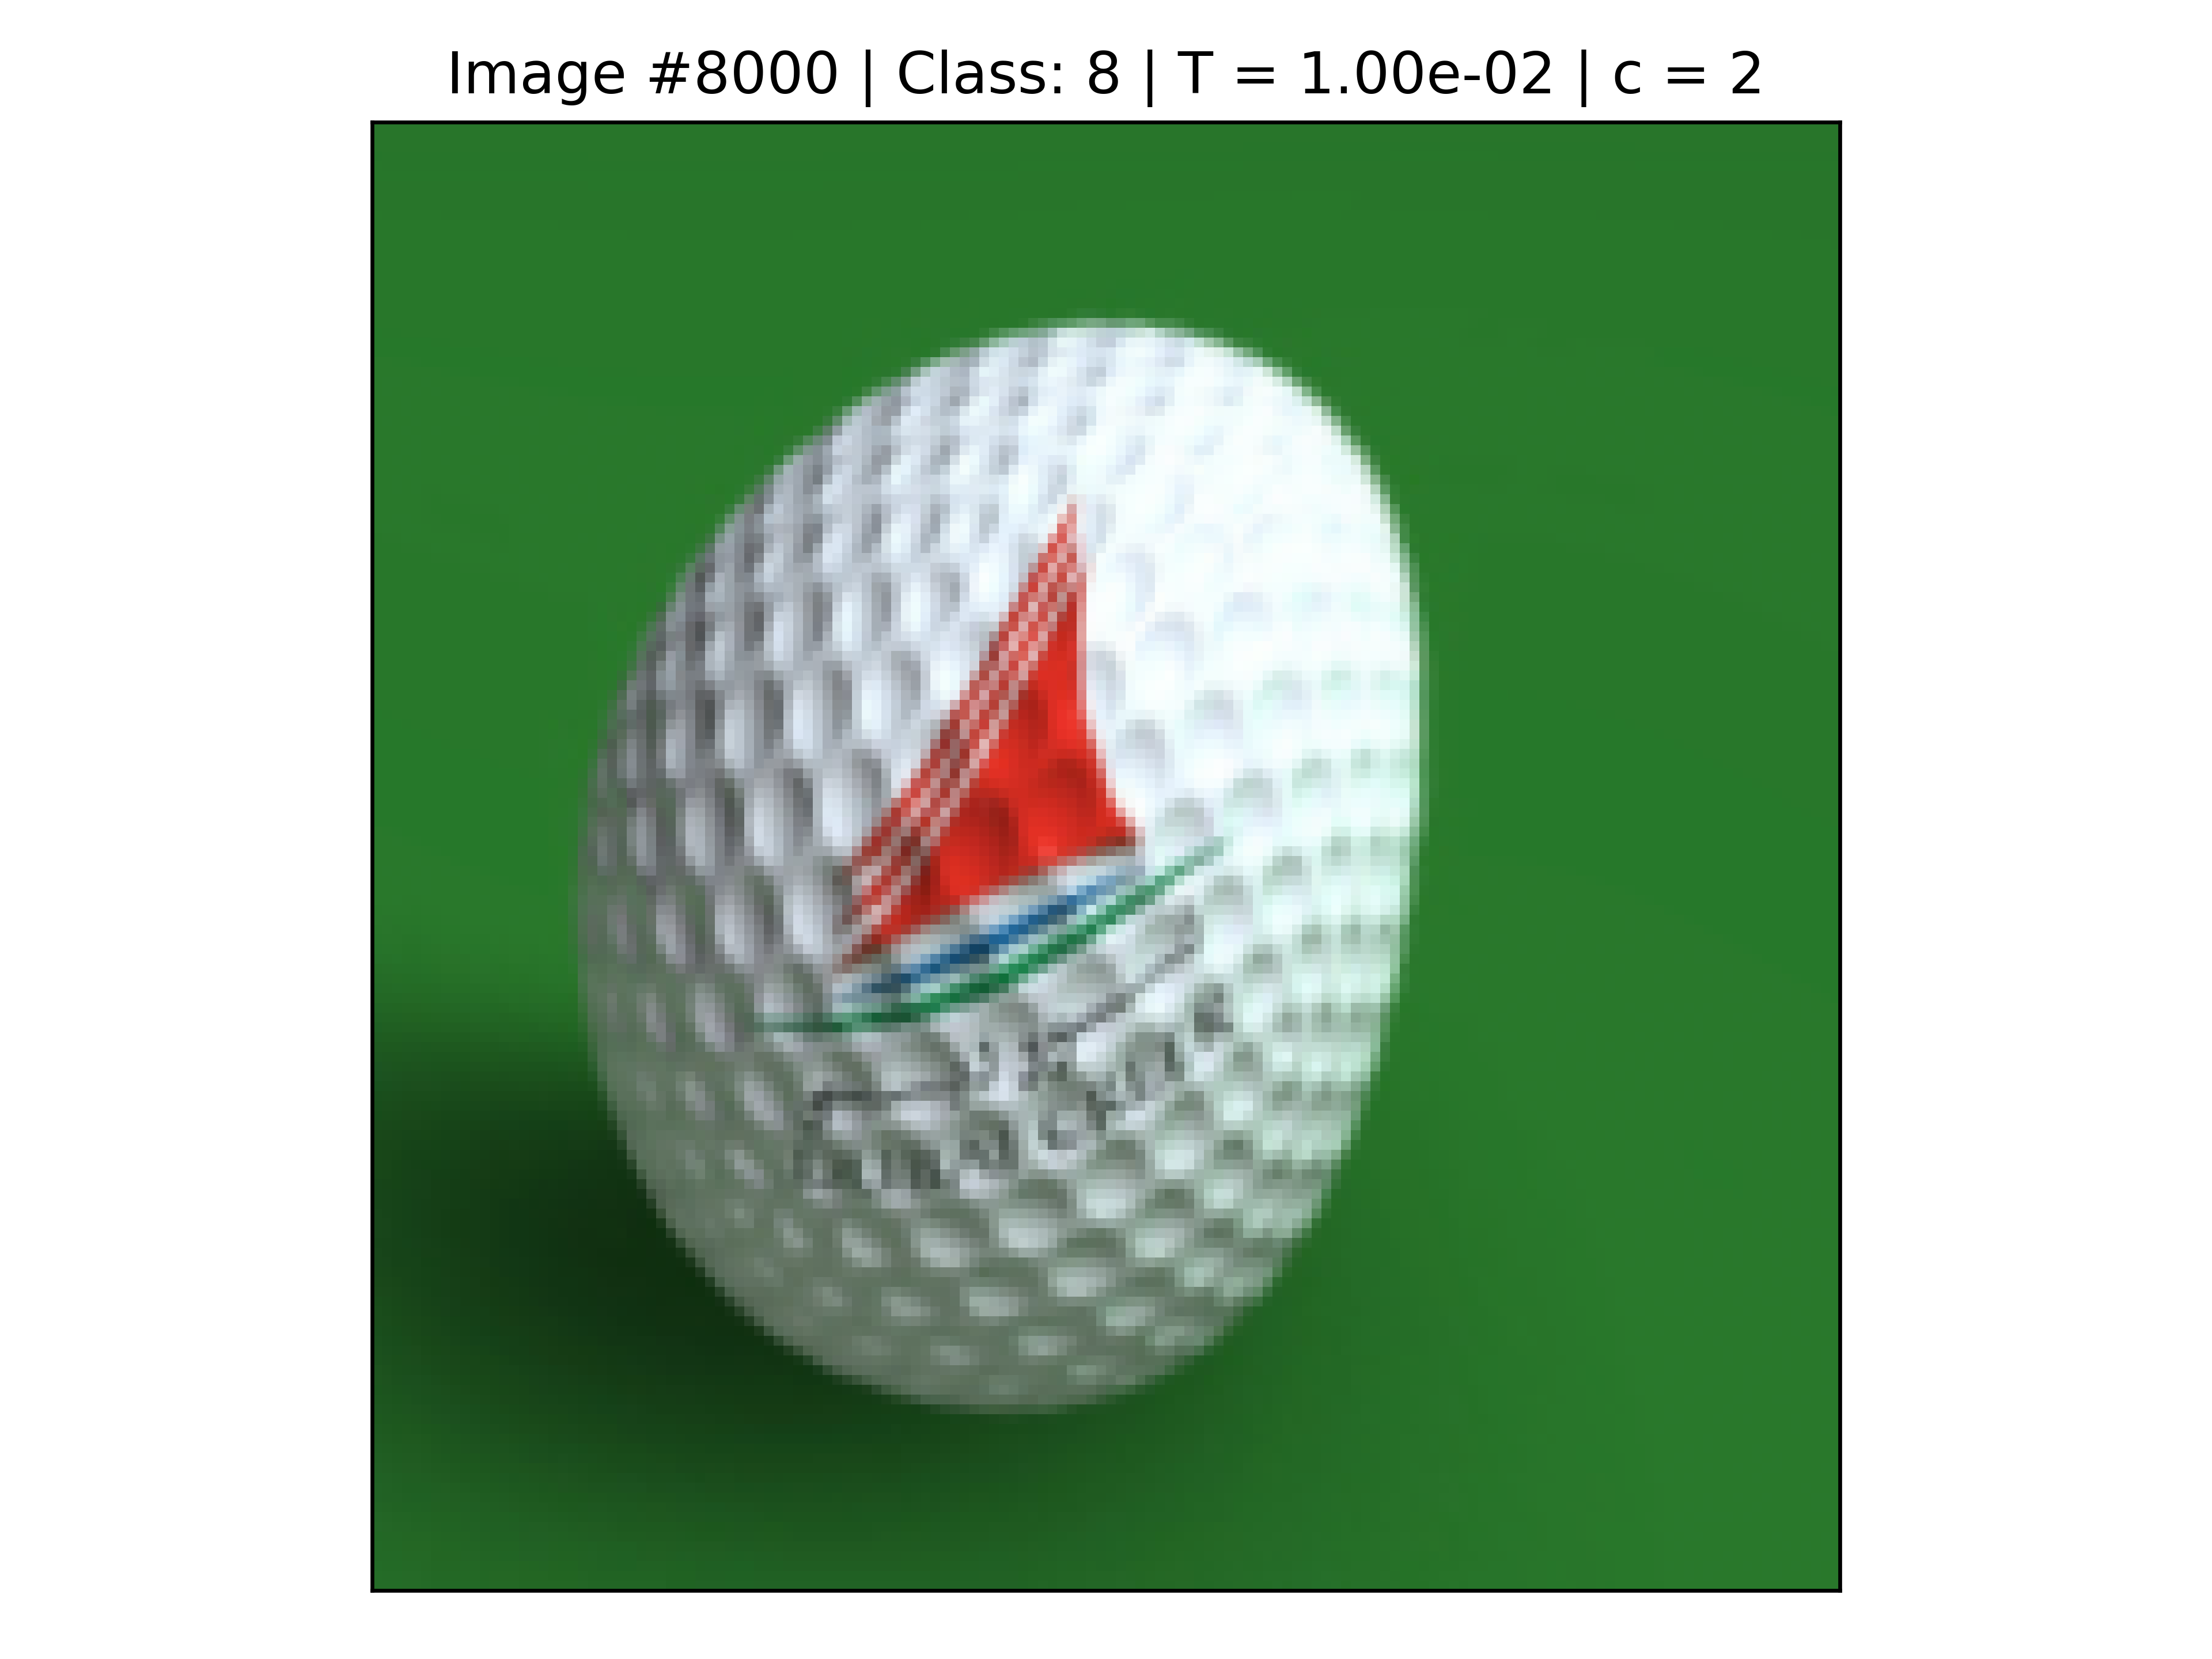
\includegraphics[width=\textwidth]{ch1-diffy/figures/warping_examples/8000_2_1.png}
%    \caption{$T=10^{-2}$}
%    % \label{fig:my_label}
%    \end{subfigure}
%    \begin{subfigure}{0.18\textwidth}
%    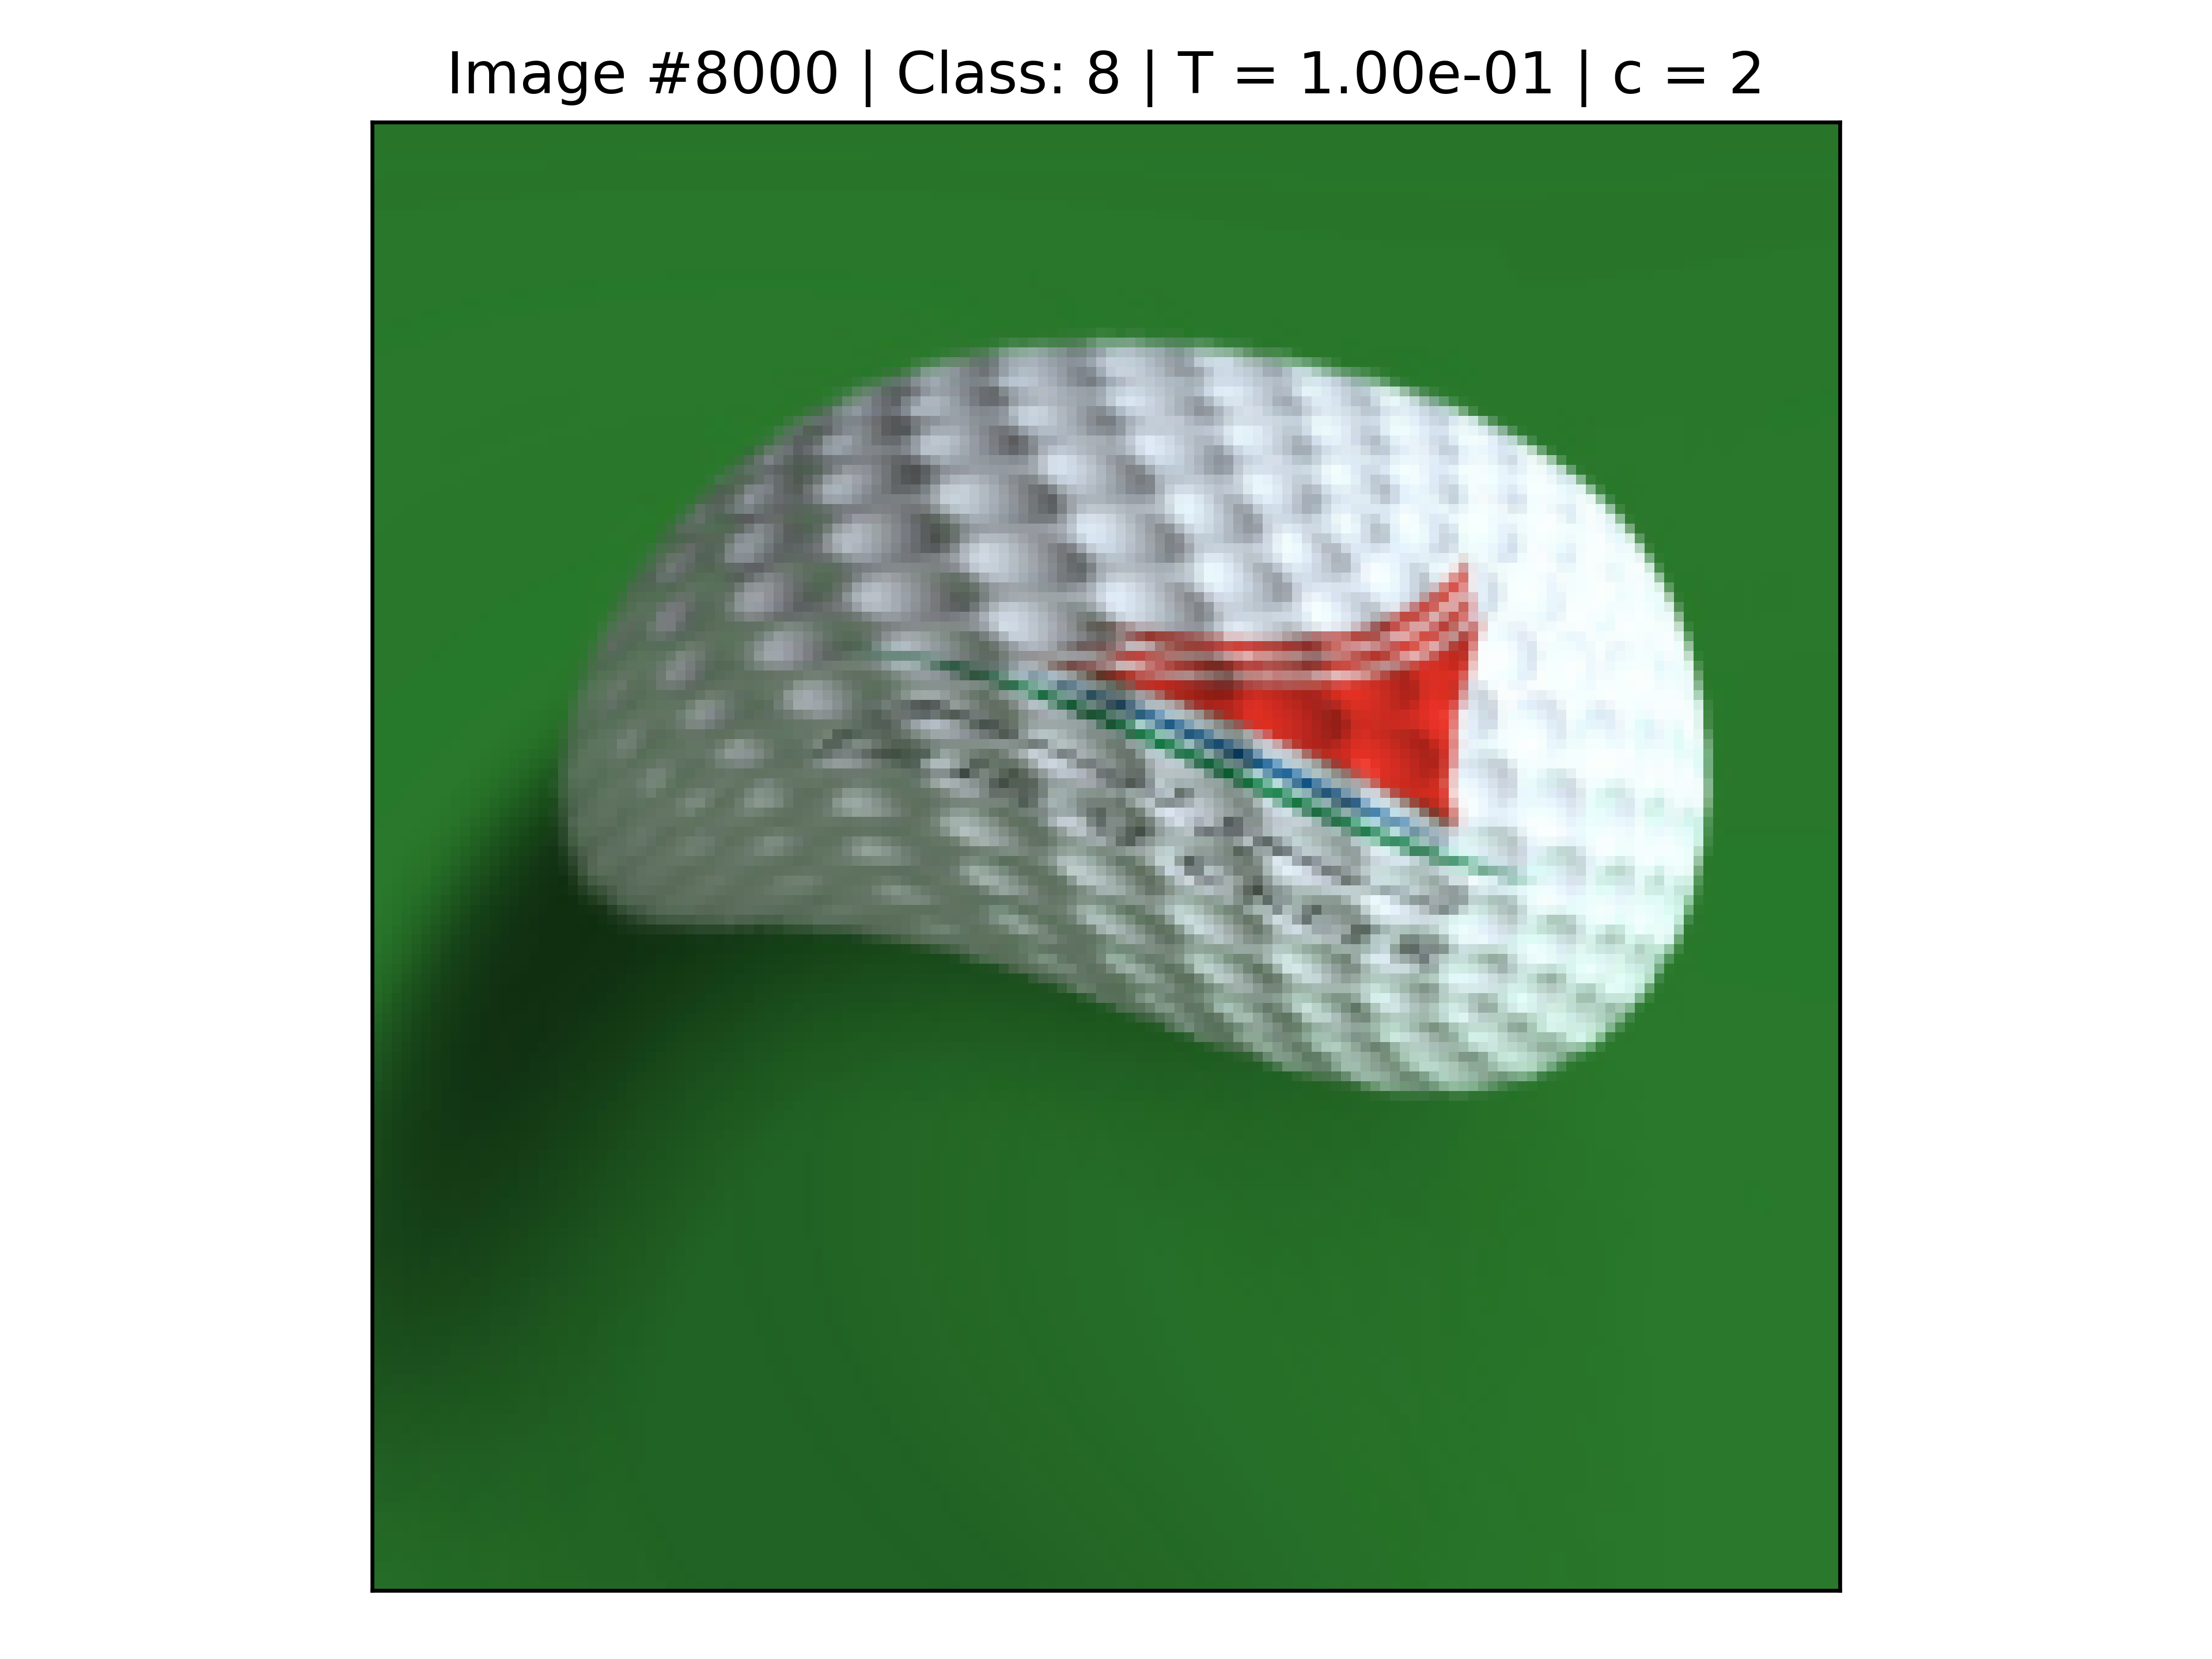
\includegraphics[width=\textwidth]{ch1-diffy/figures/warping_examples/8000_1_1.png}
%    \caption{$T=10^{-1}$}
%    % \label{fig:my_label}
%    \end{subfigure}
%    \begin{subfigure}{0.18\textwidth}
%    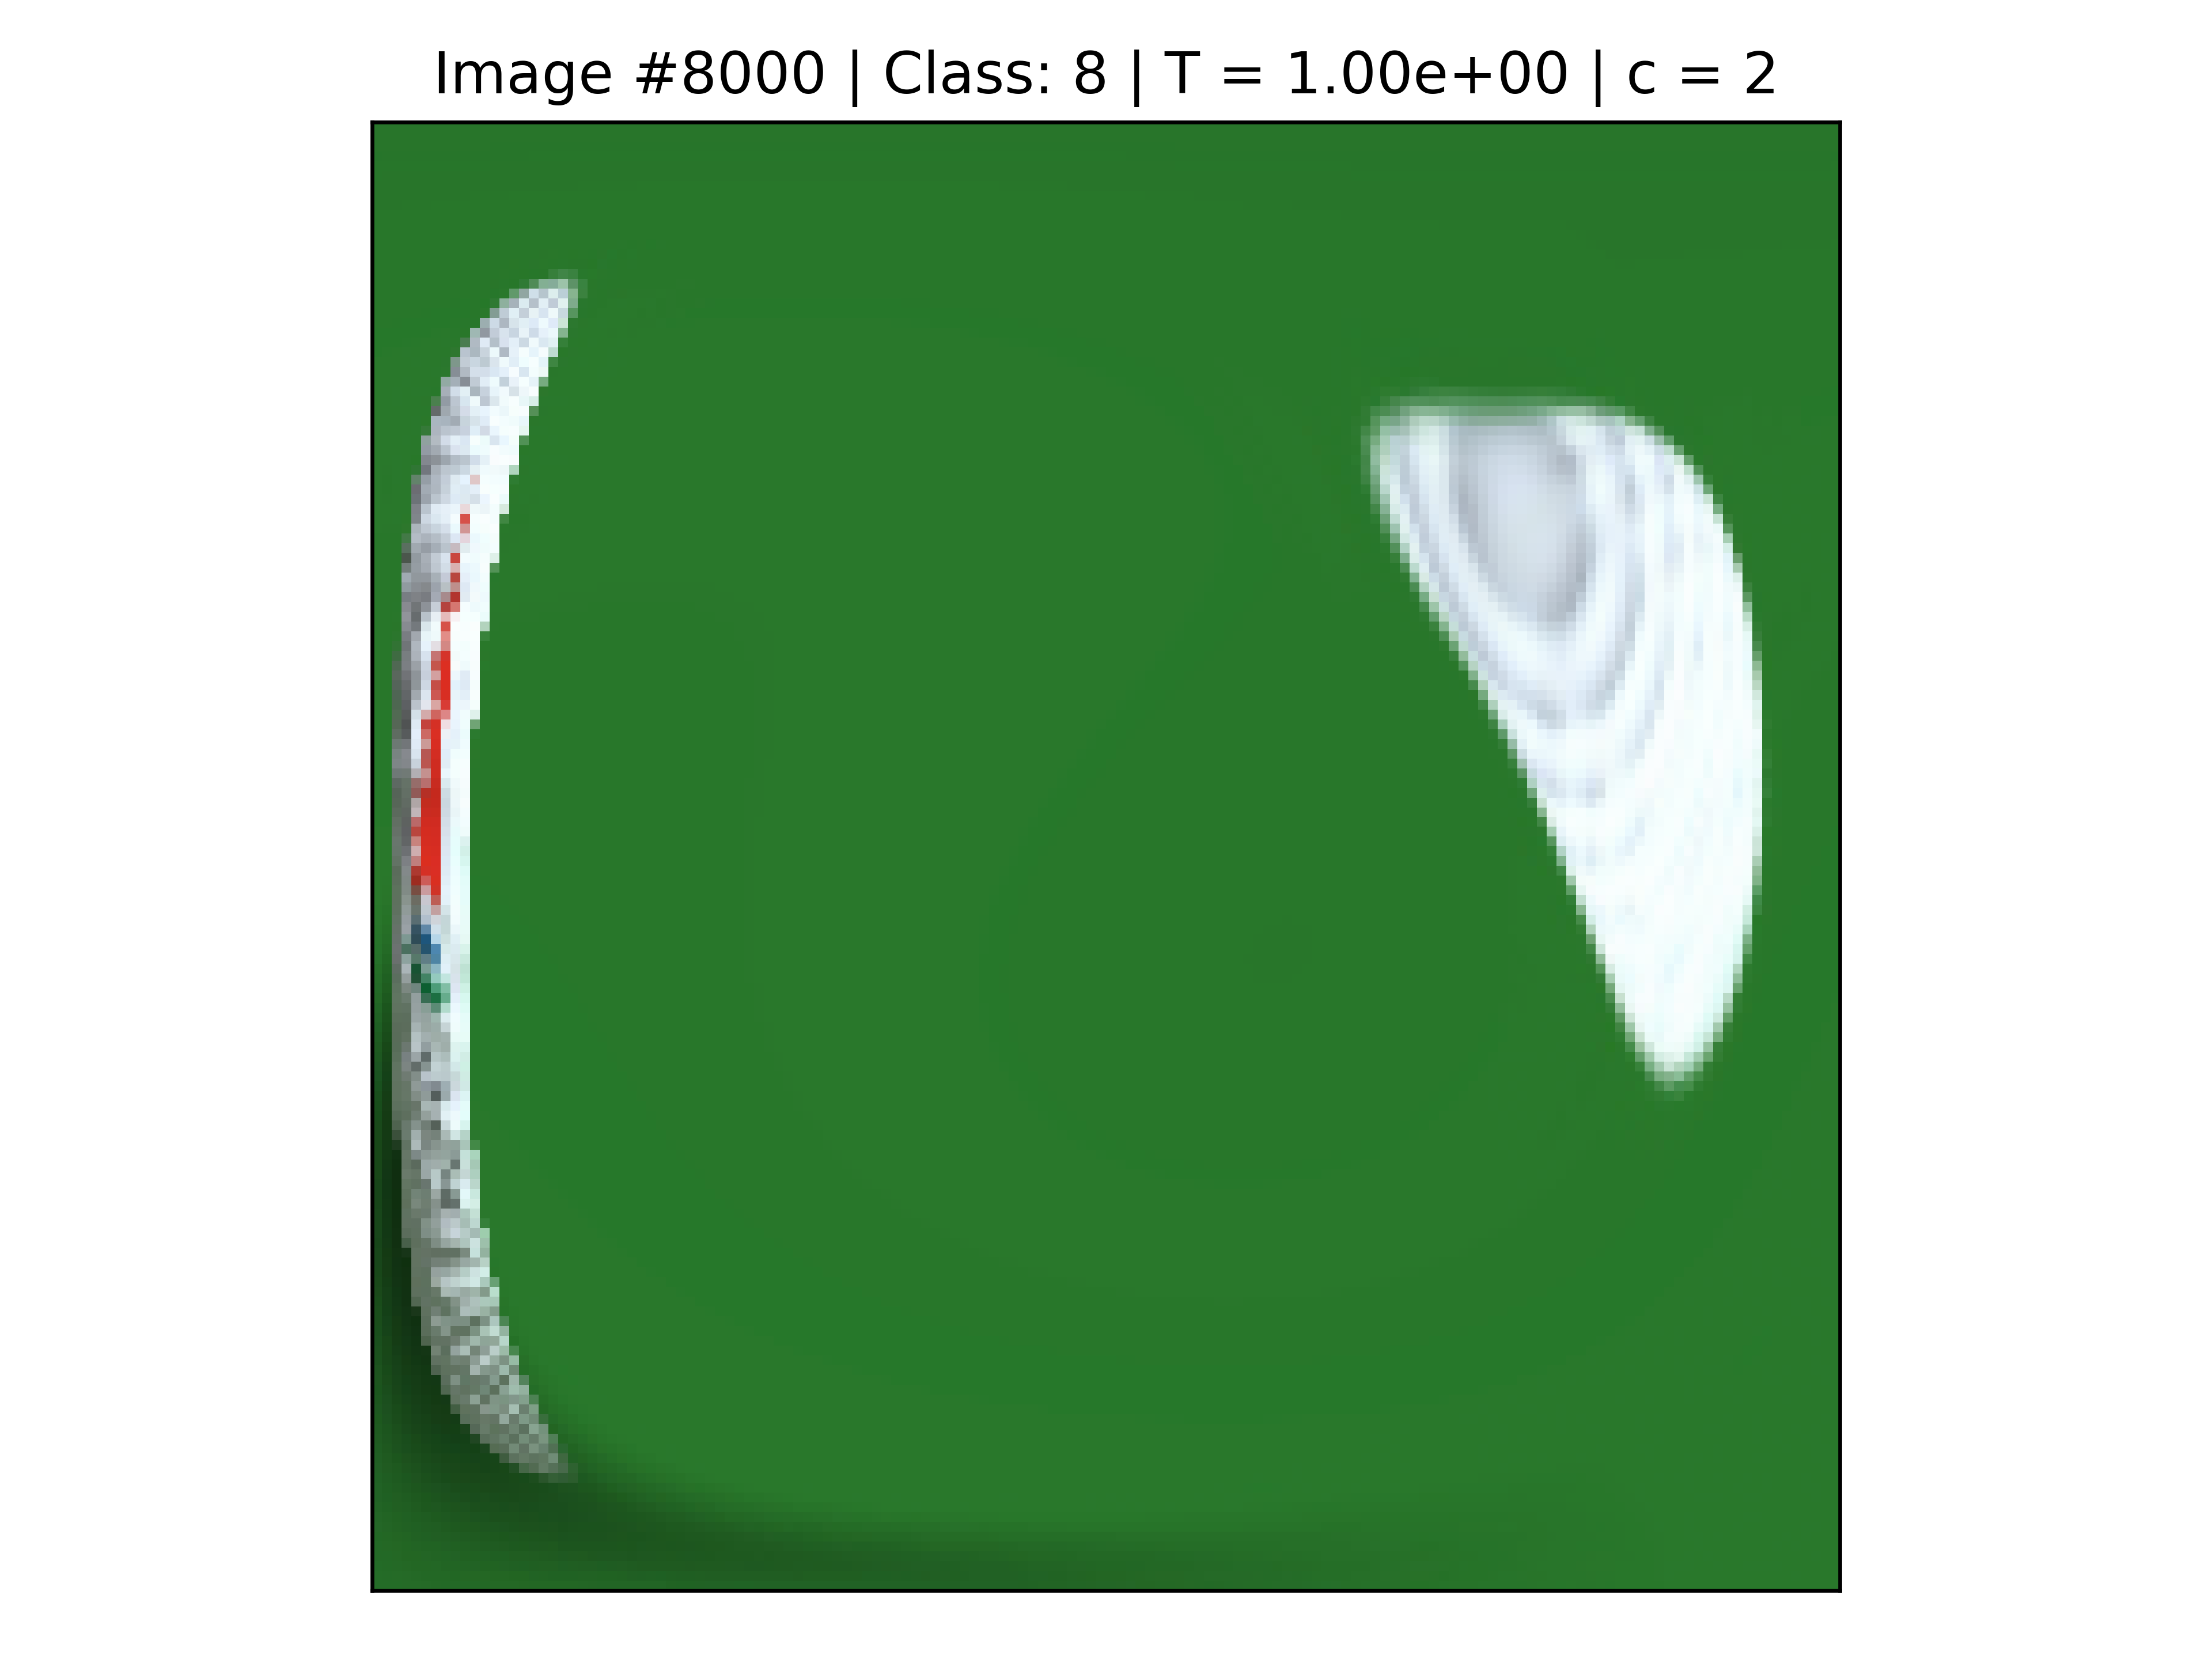
\includegraphics[width=\textwidth]{ch1-diffy/figures/warping_examples/8000_0_1.png}
%    \caption{$T=1$}
%    % \label{fig:my_label}
%    \end{subfigure}
%    \begin{subfigure}{0.18\textwidth}
%    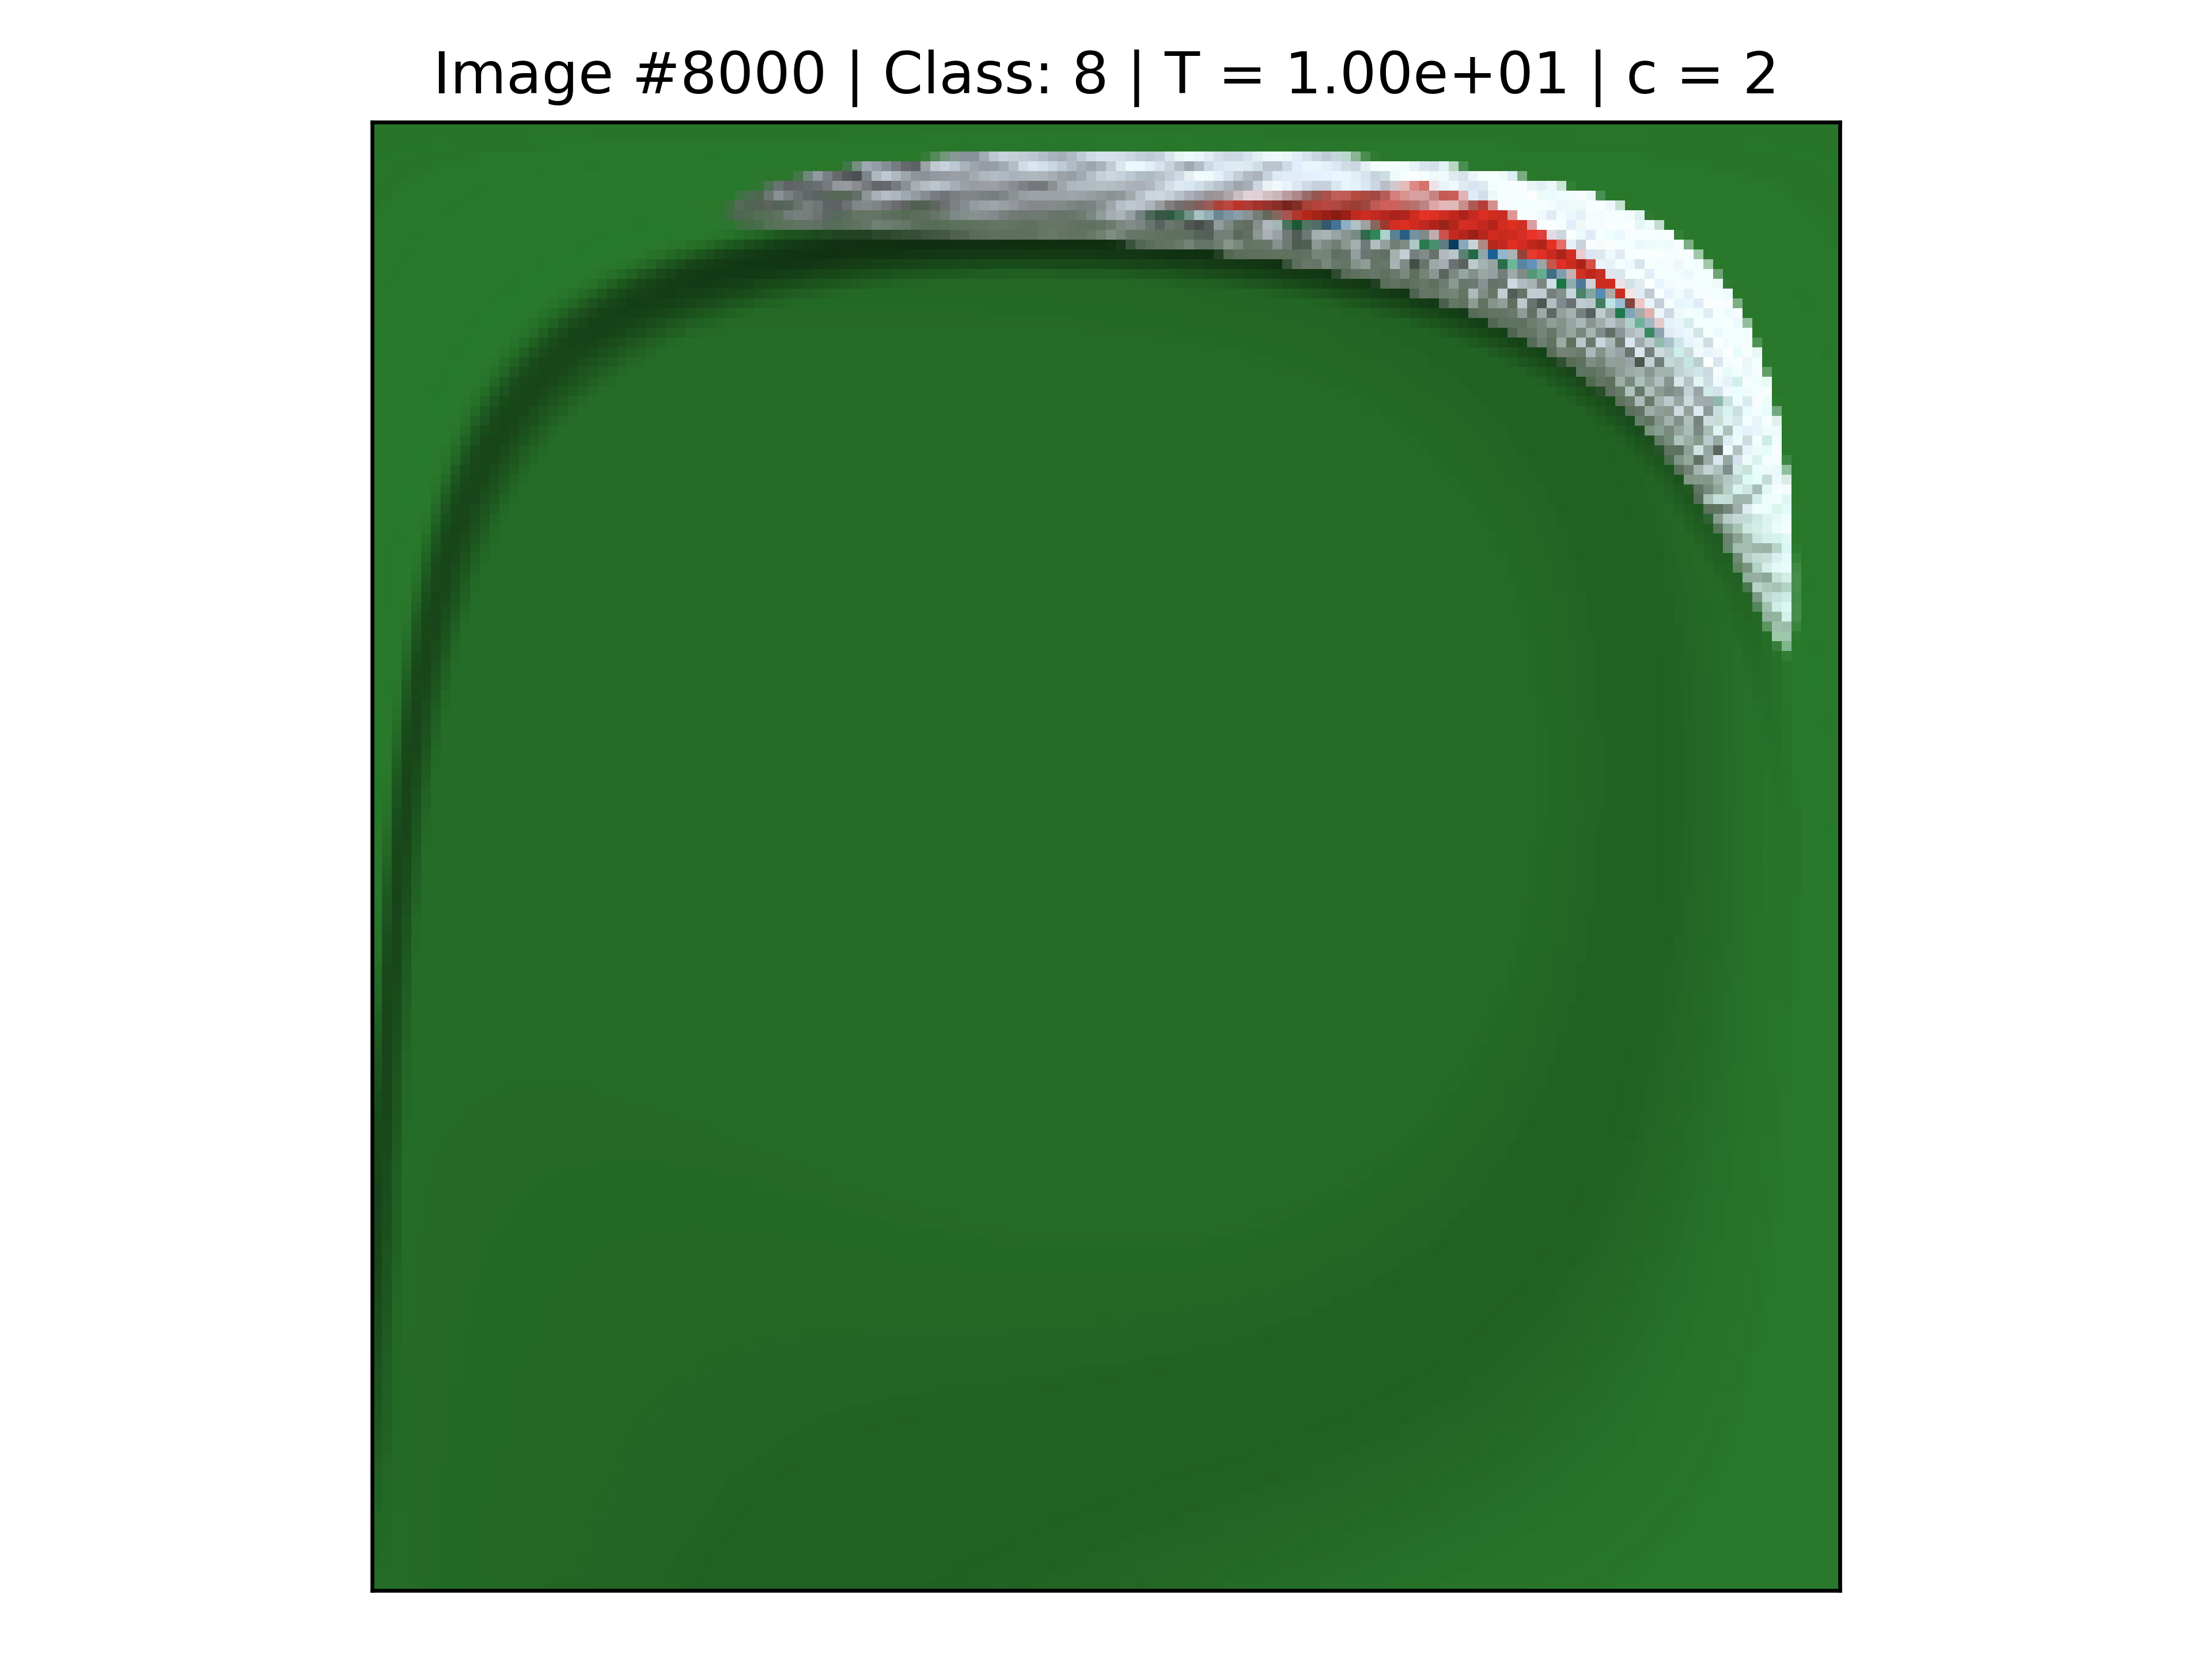
\includegraphics[width=\textwidth]{ch1-diffy/figures/warping_examples/8000_-1_1.png}
%    \caption{$T=10$}
%    % \label{fig:my_label}
%    \end{subfigure}
%    %%%%%
%    \begin{subfigure}{0.18\textwidth}
%    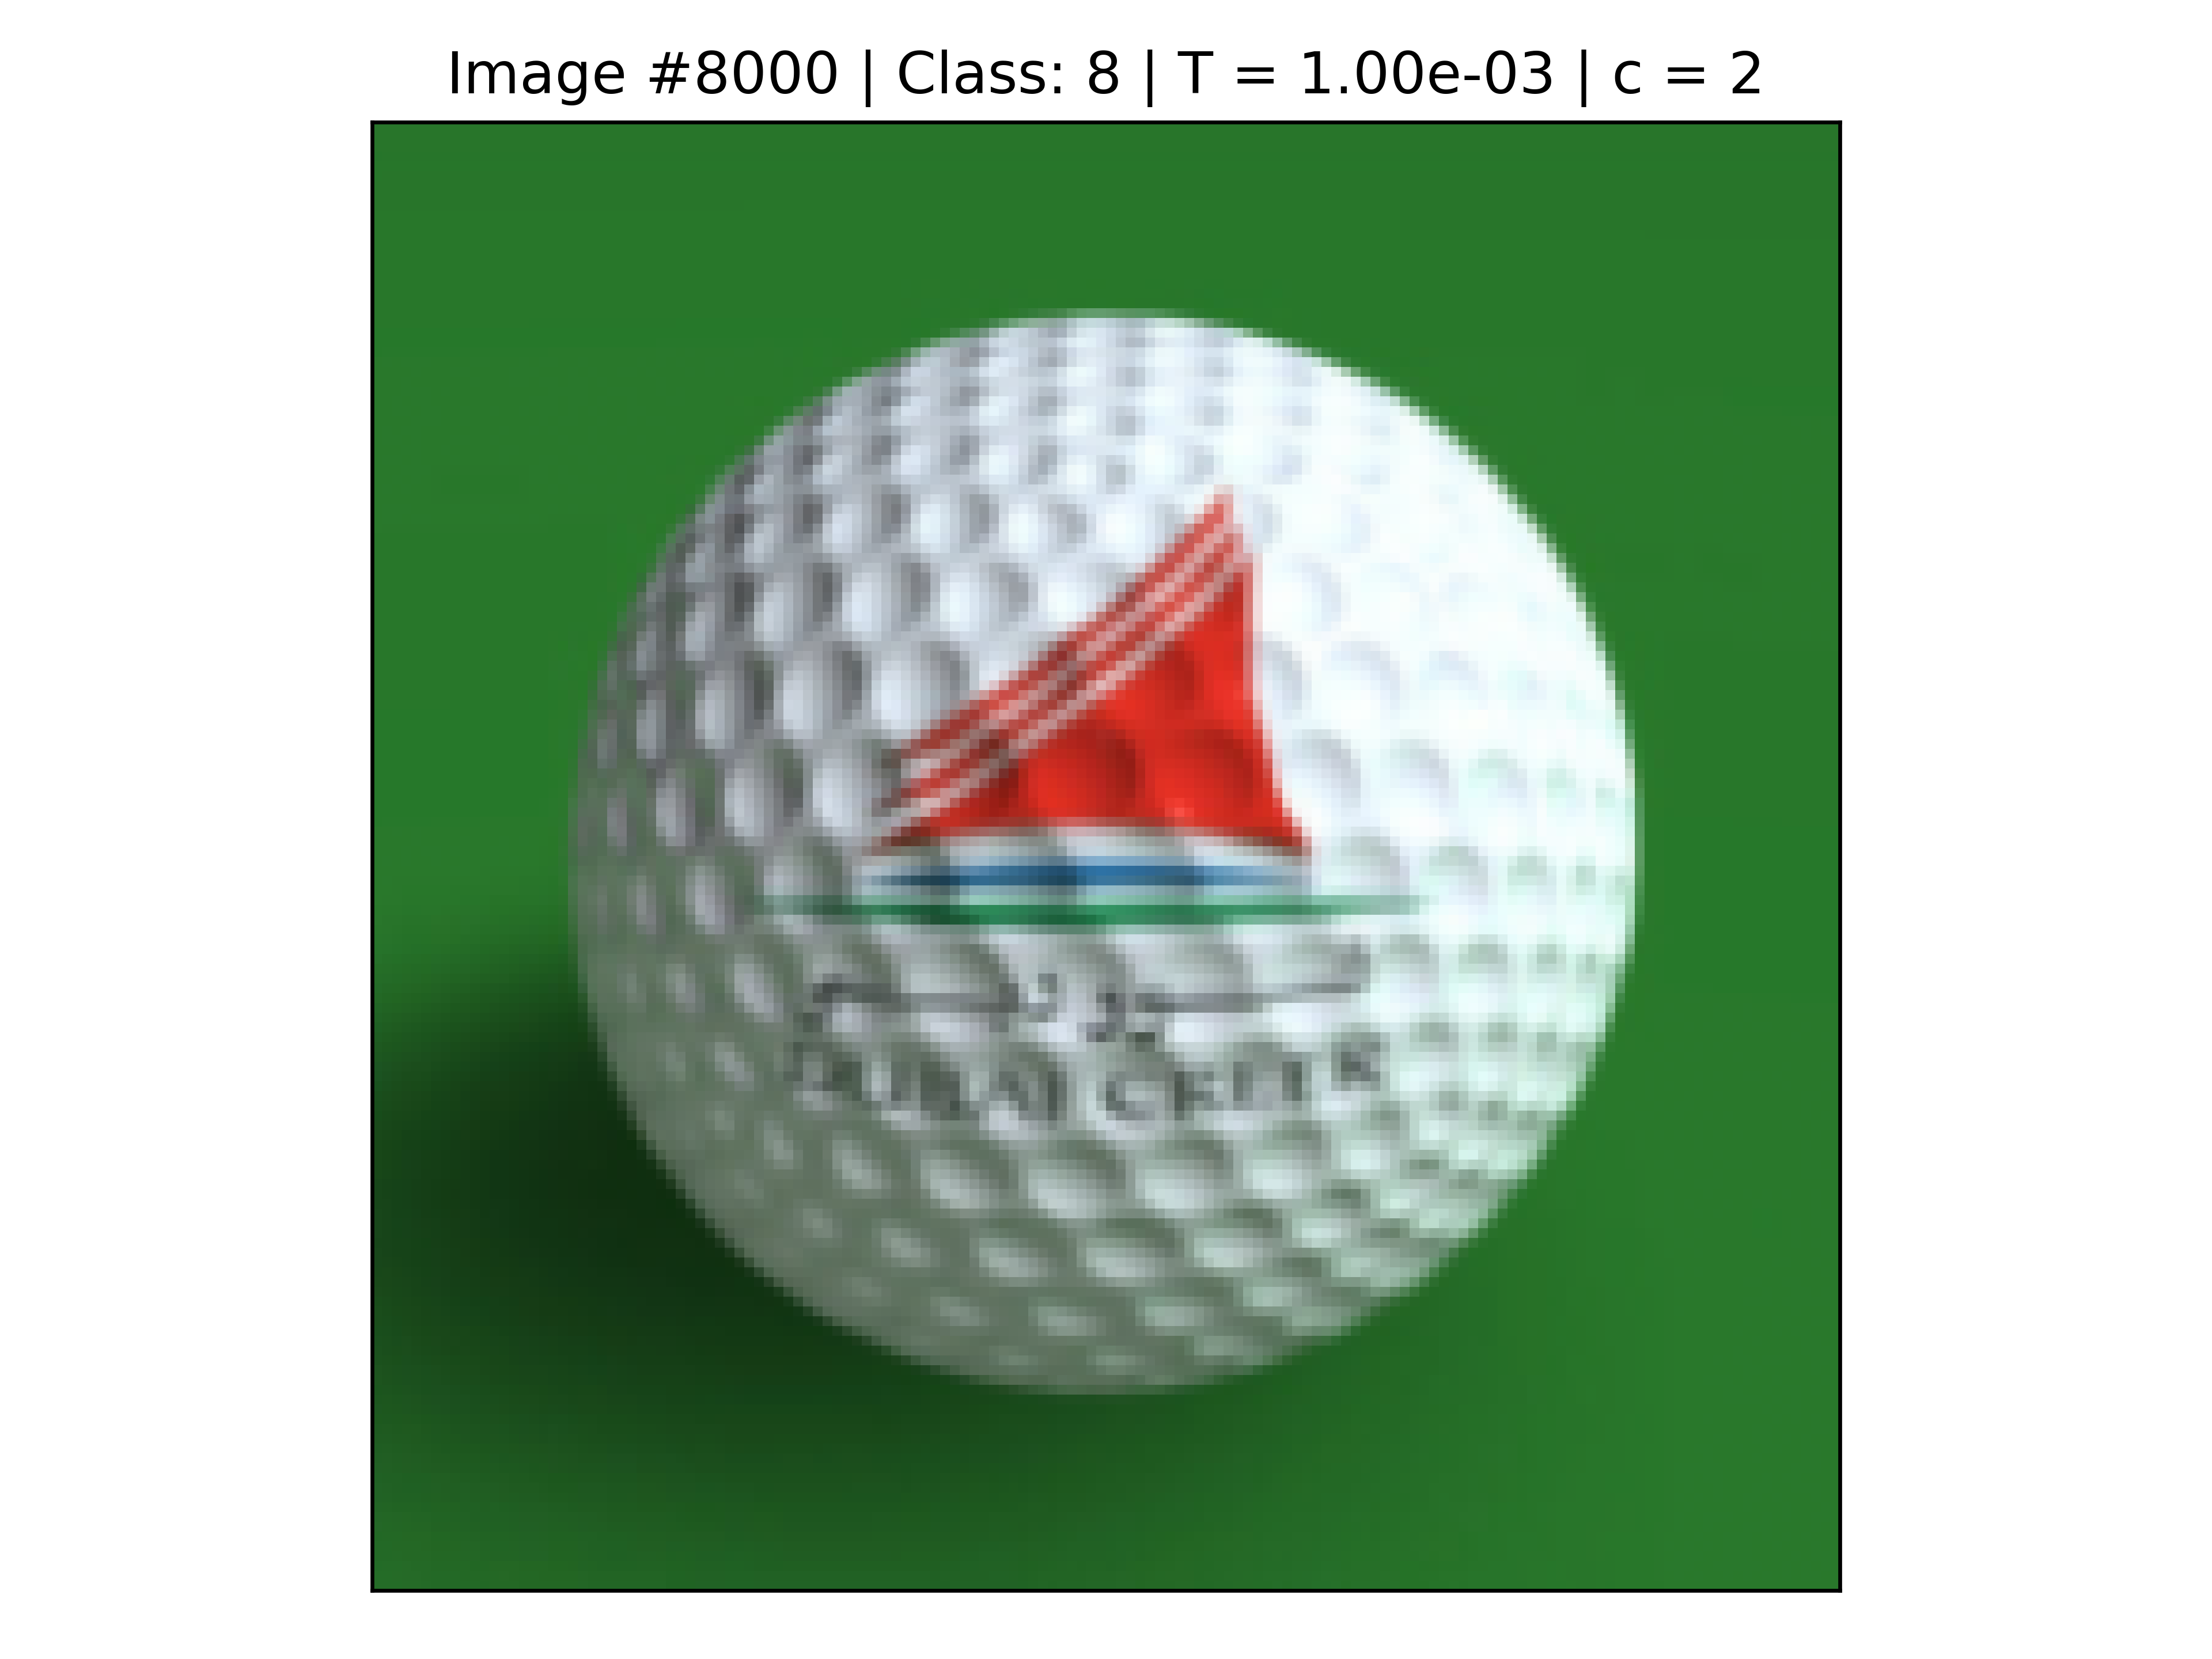
\includegraphics[width=\textwidth]{ch1-diffy/figures/warping_examples/8000_3_2.png}
%    \caption{$T=10^{-3}$}
%    % \label{fig:my_label}
%    \end{subfigure}
%    \begin{subfigure}{0.18\textwidth}
%    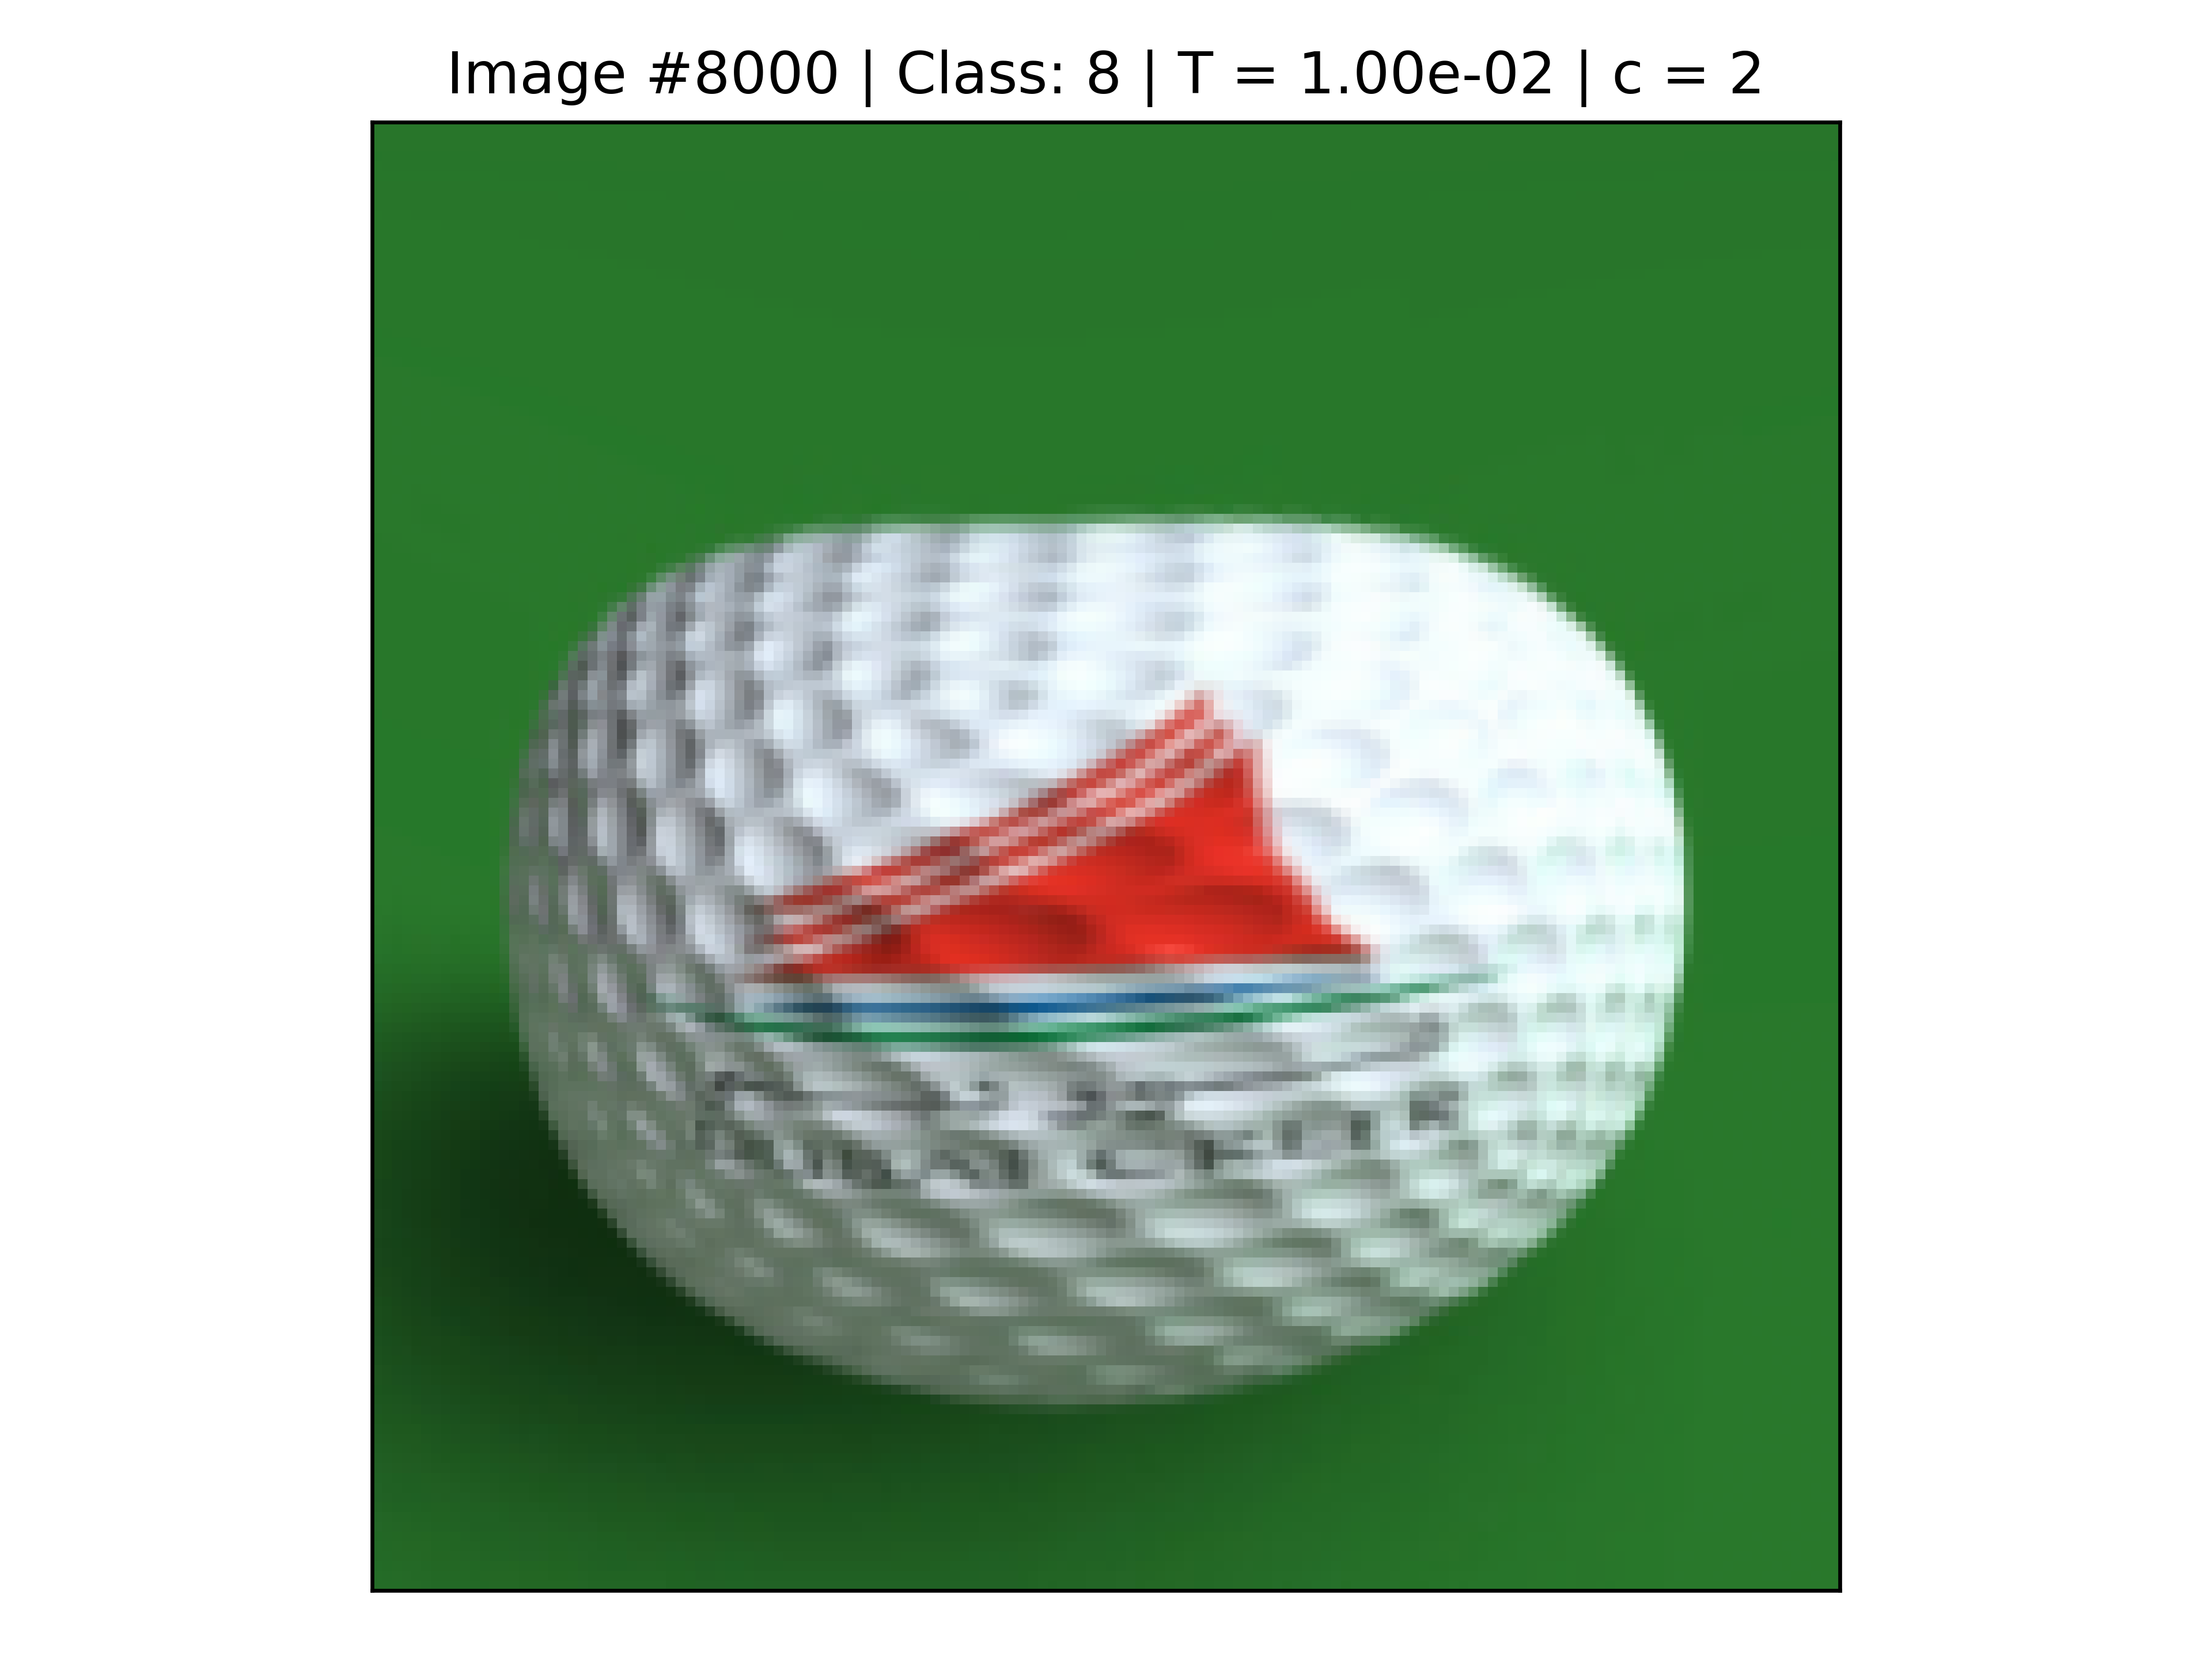
\includegraphics[width=\textwidth]{ch1-diffy/figures/warping_examples/8000_2_2.png}
%    \caption{$T=10^{-2}$}
%    % \label{fig:my_label}
%    \end{subfigure}
%    \begin{subfigure}{0.18\textwidth}
%    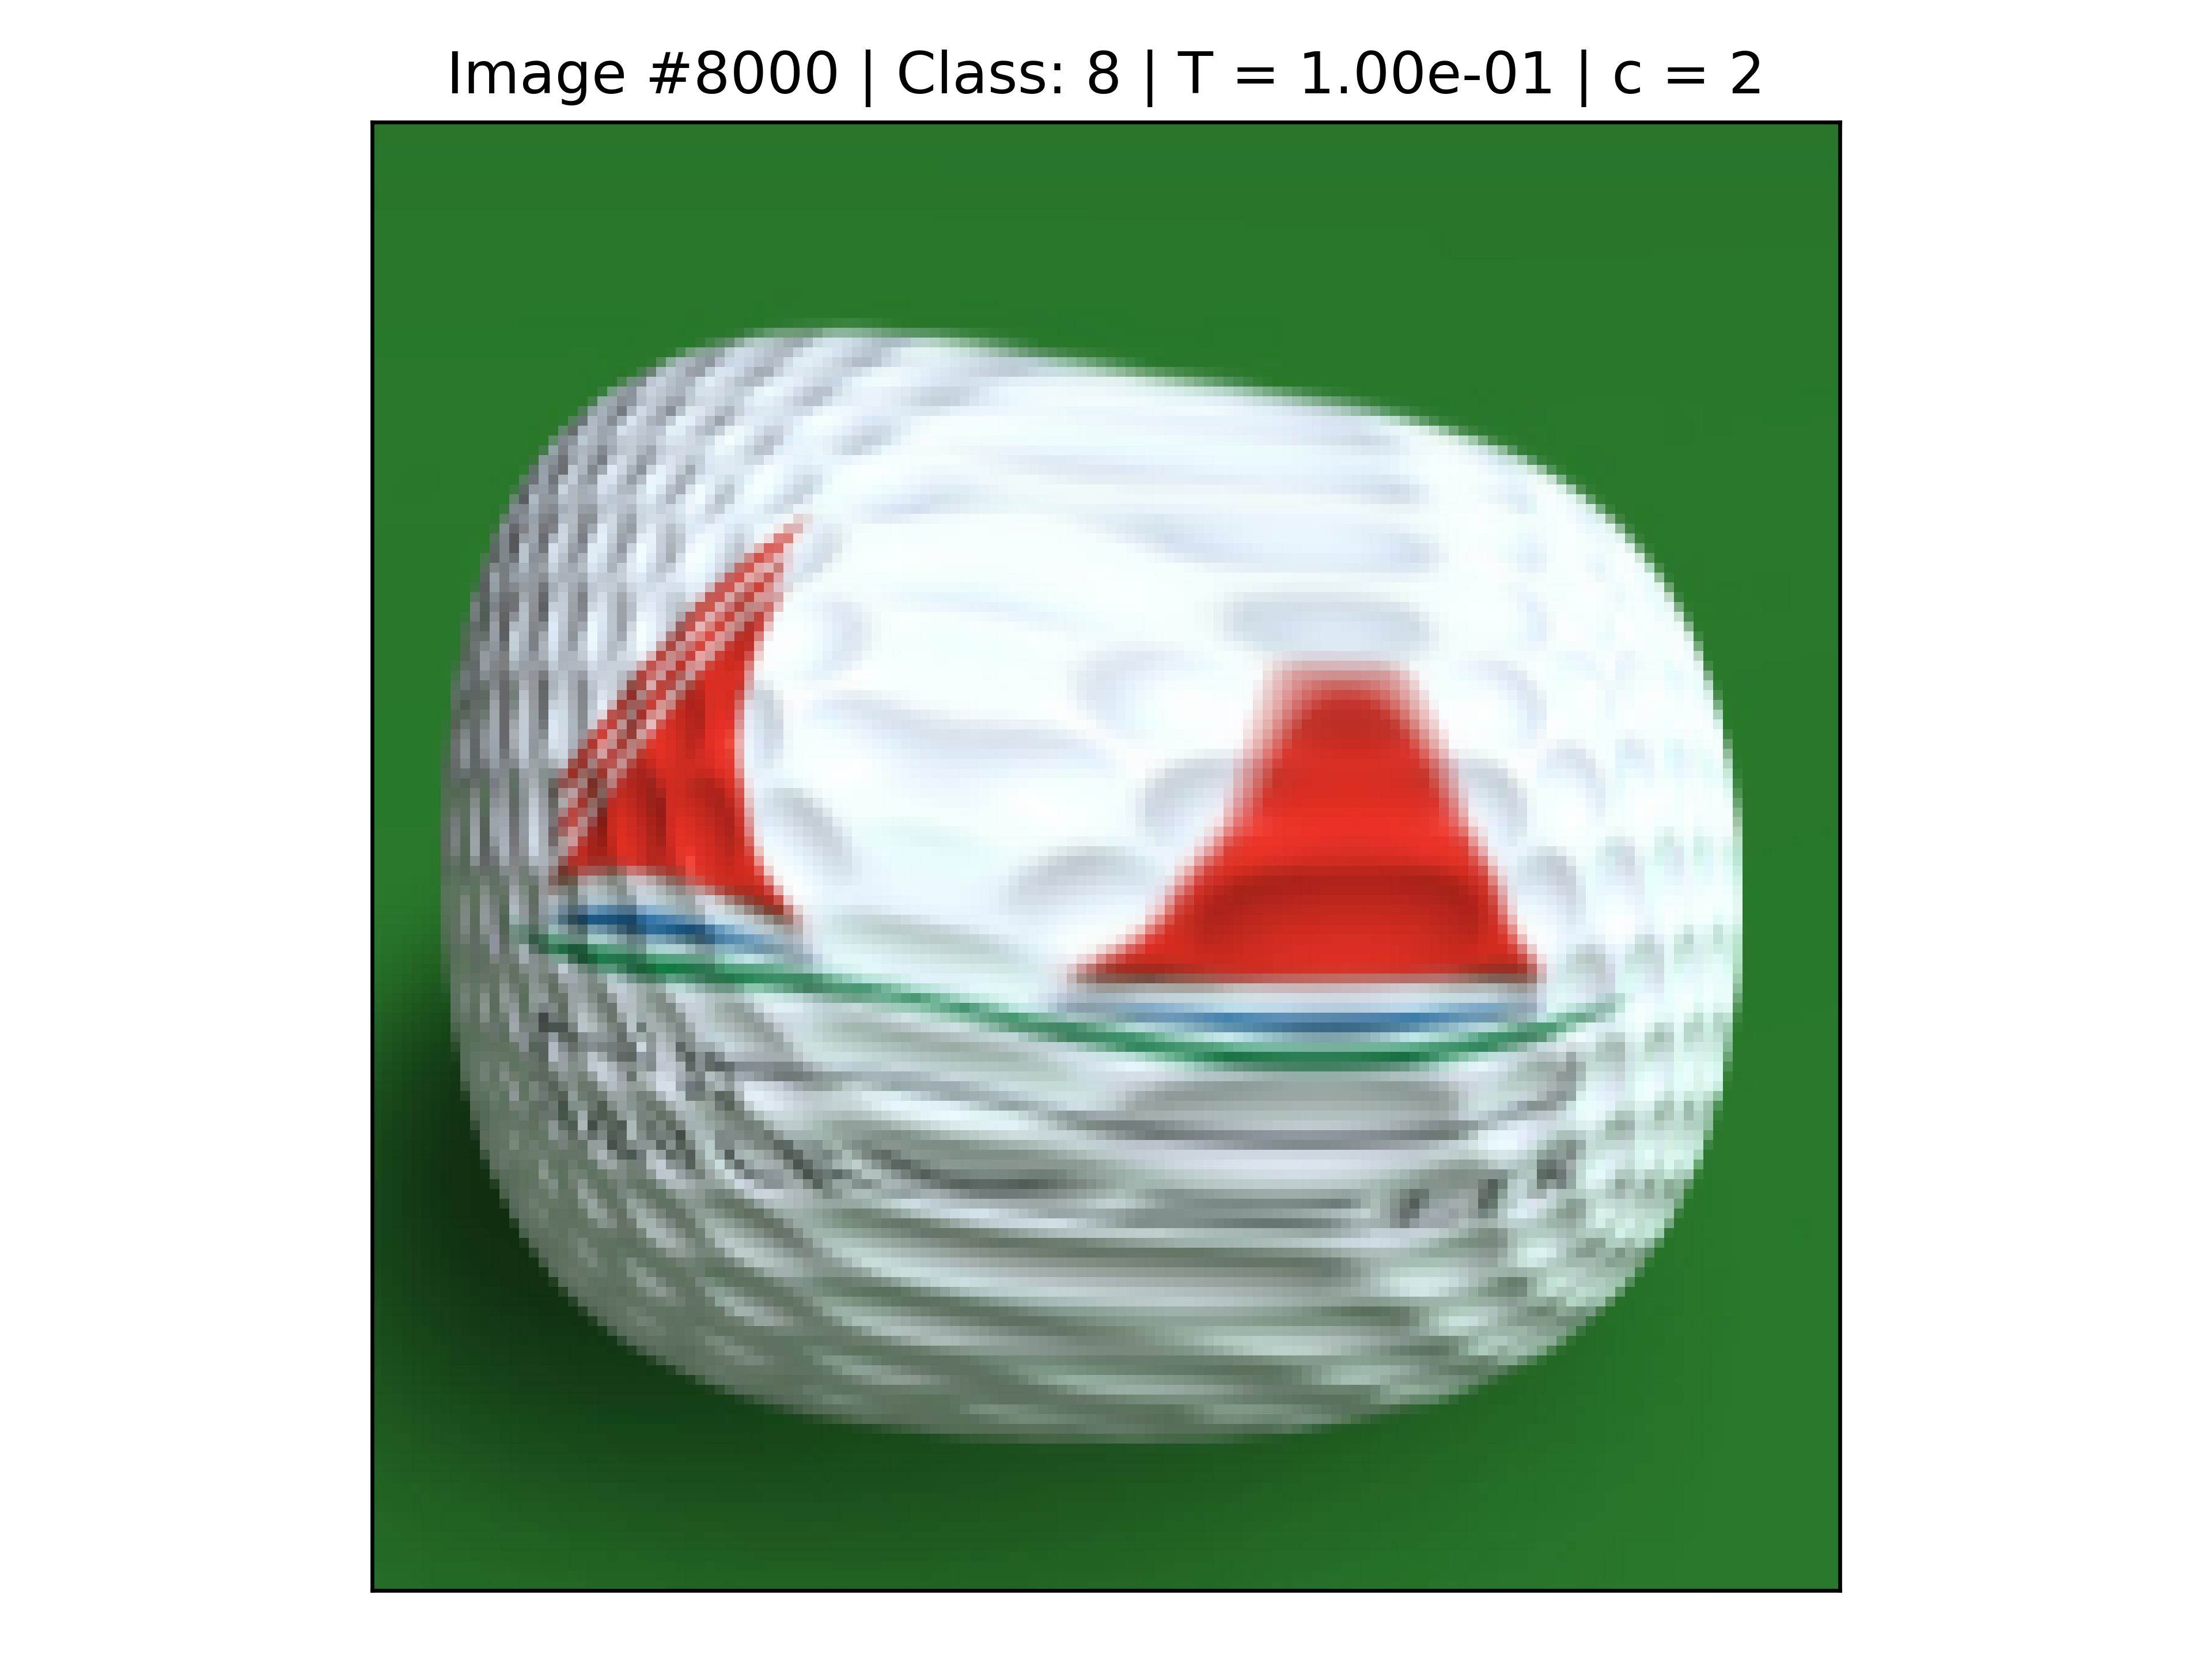
\includegraphics[width=\textwidth]{ch1-diffy/figures/warping_examples/8000_1_2.png}
%    \caption{$T=10^{-1}$}
%    % \label{fig:my_label}
%    \end{subfigure}
%    \begin{subfigure}{0.18\textwidth}
%    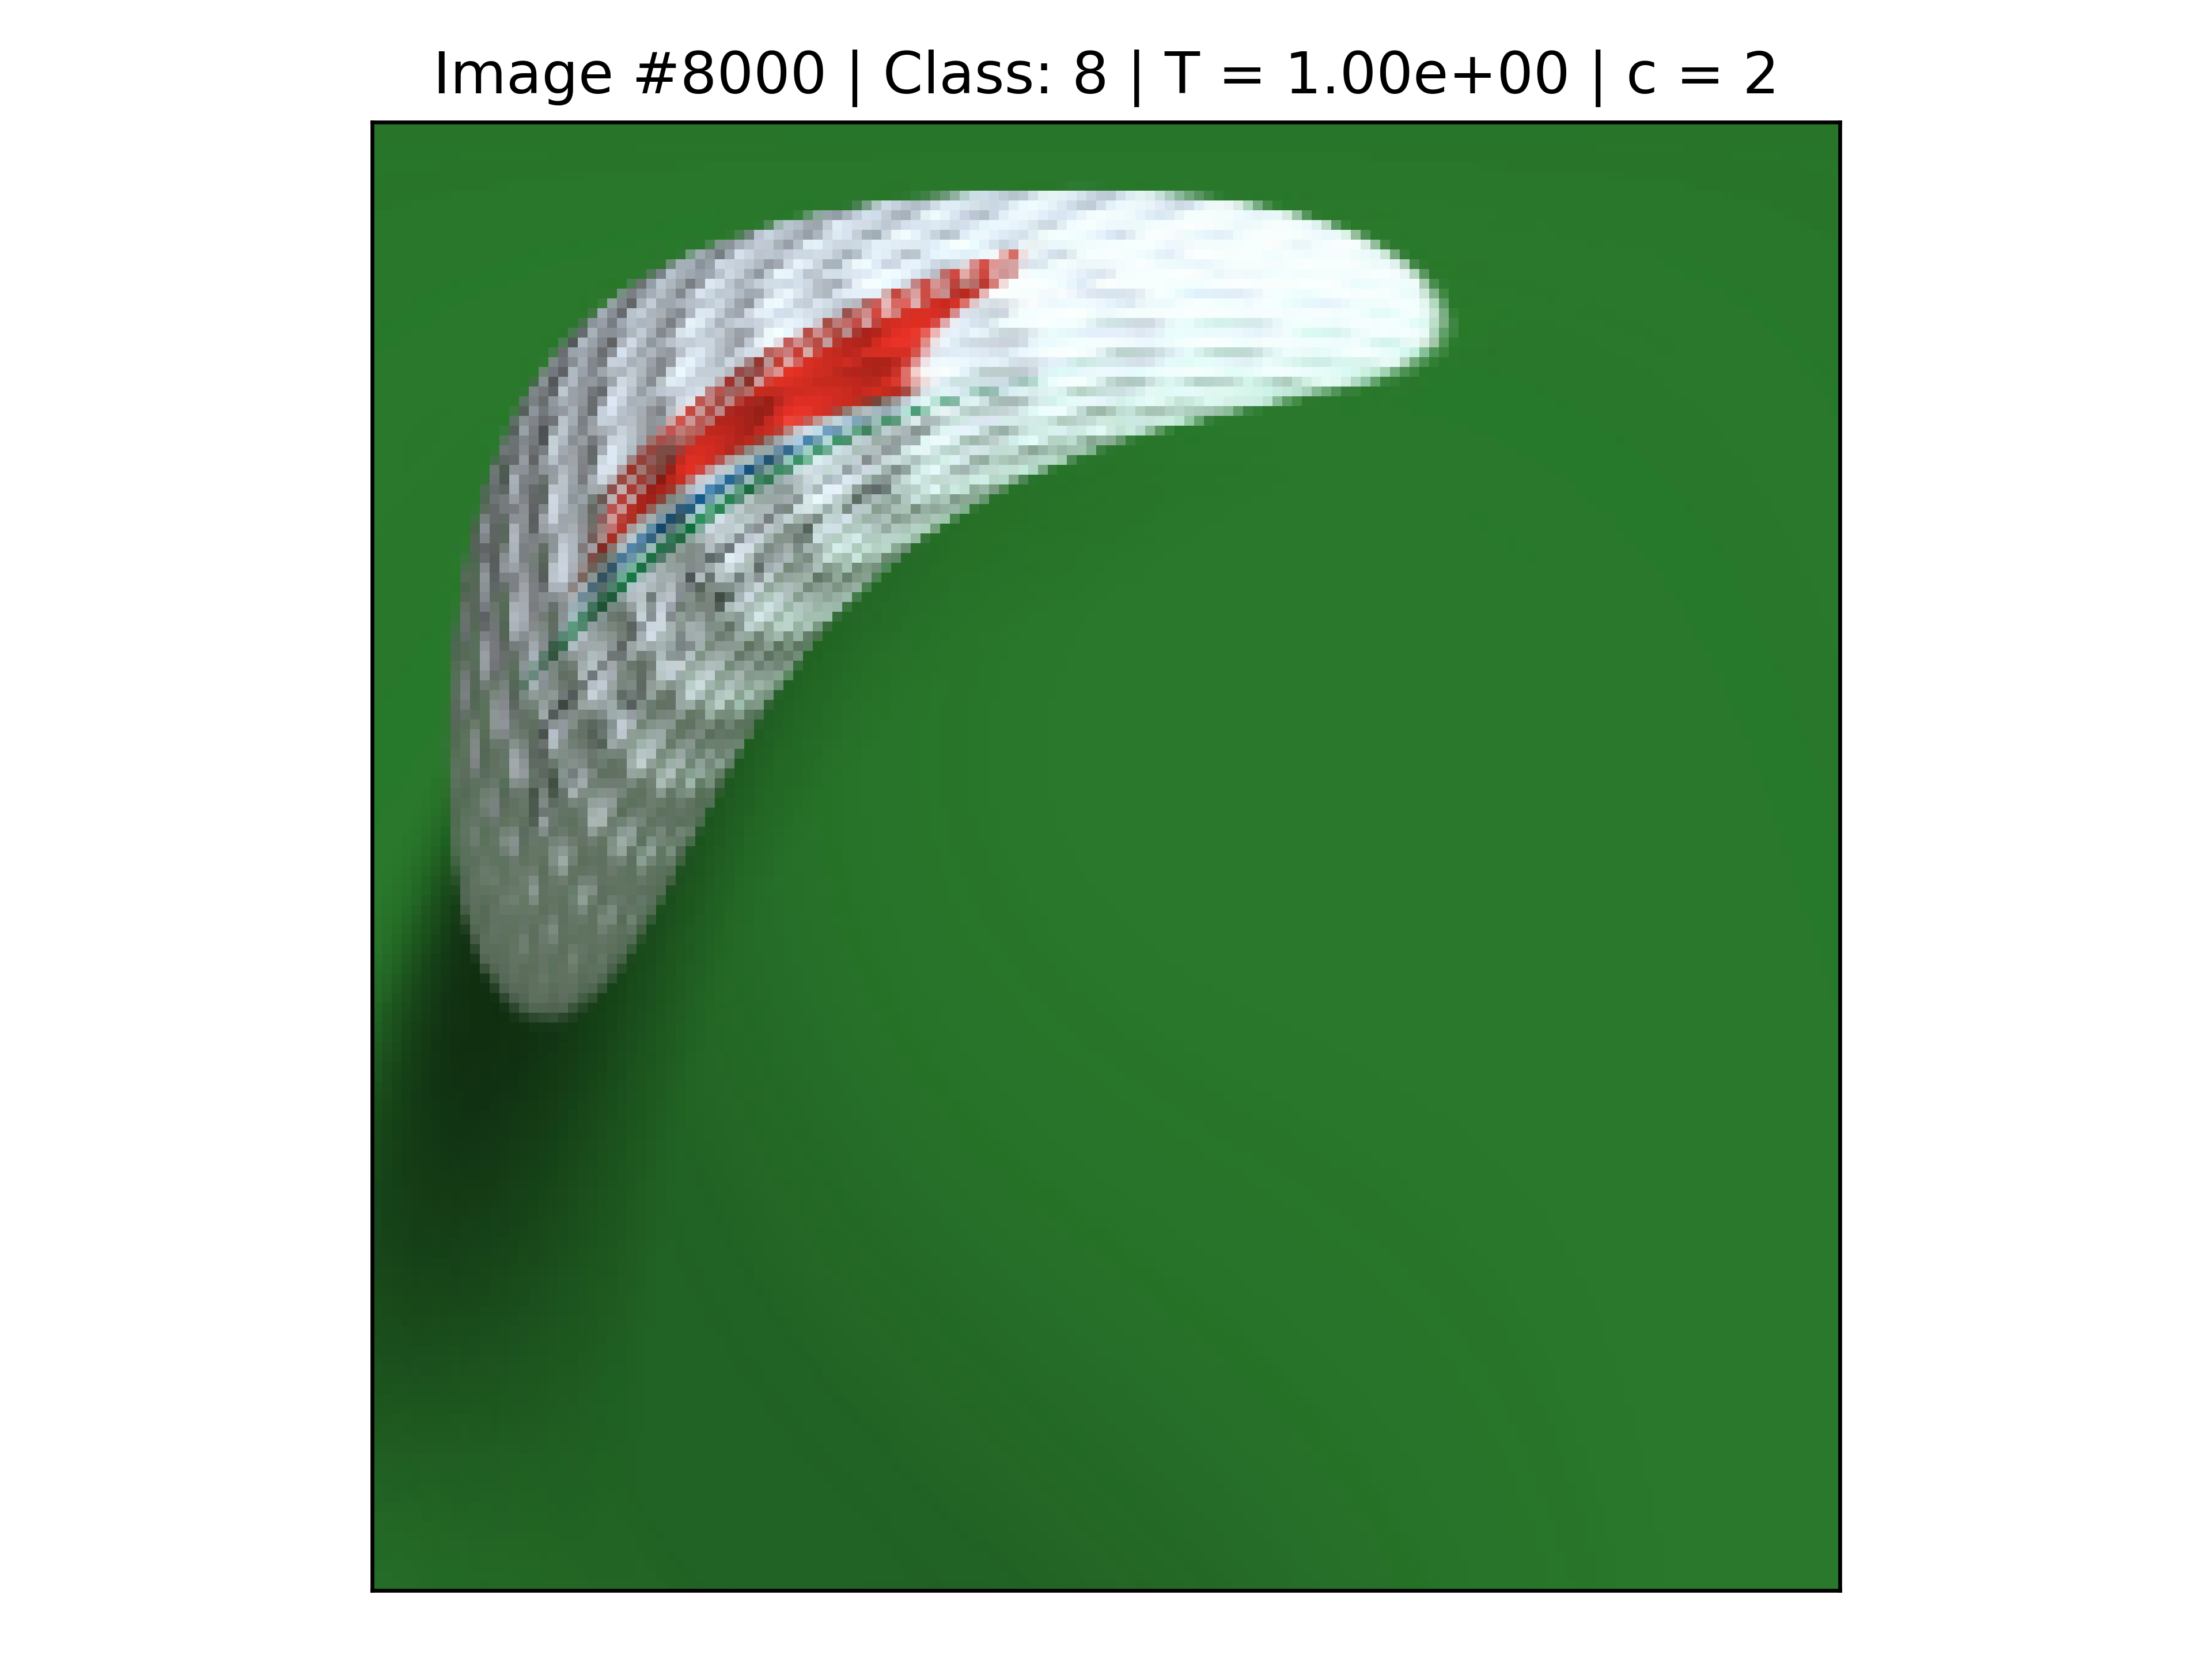
\includegraphics[width=\textwidth]{ch1-diffy/figures/warping_examples/8000_0_2.png}
%    \caption{$T=1$}
%    % \label{fig:my_label}
%    \end{subfigure}
%    \begin{subfigure}{0.18\textwidth}
%    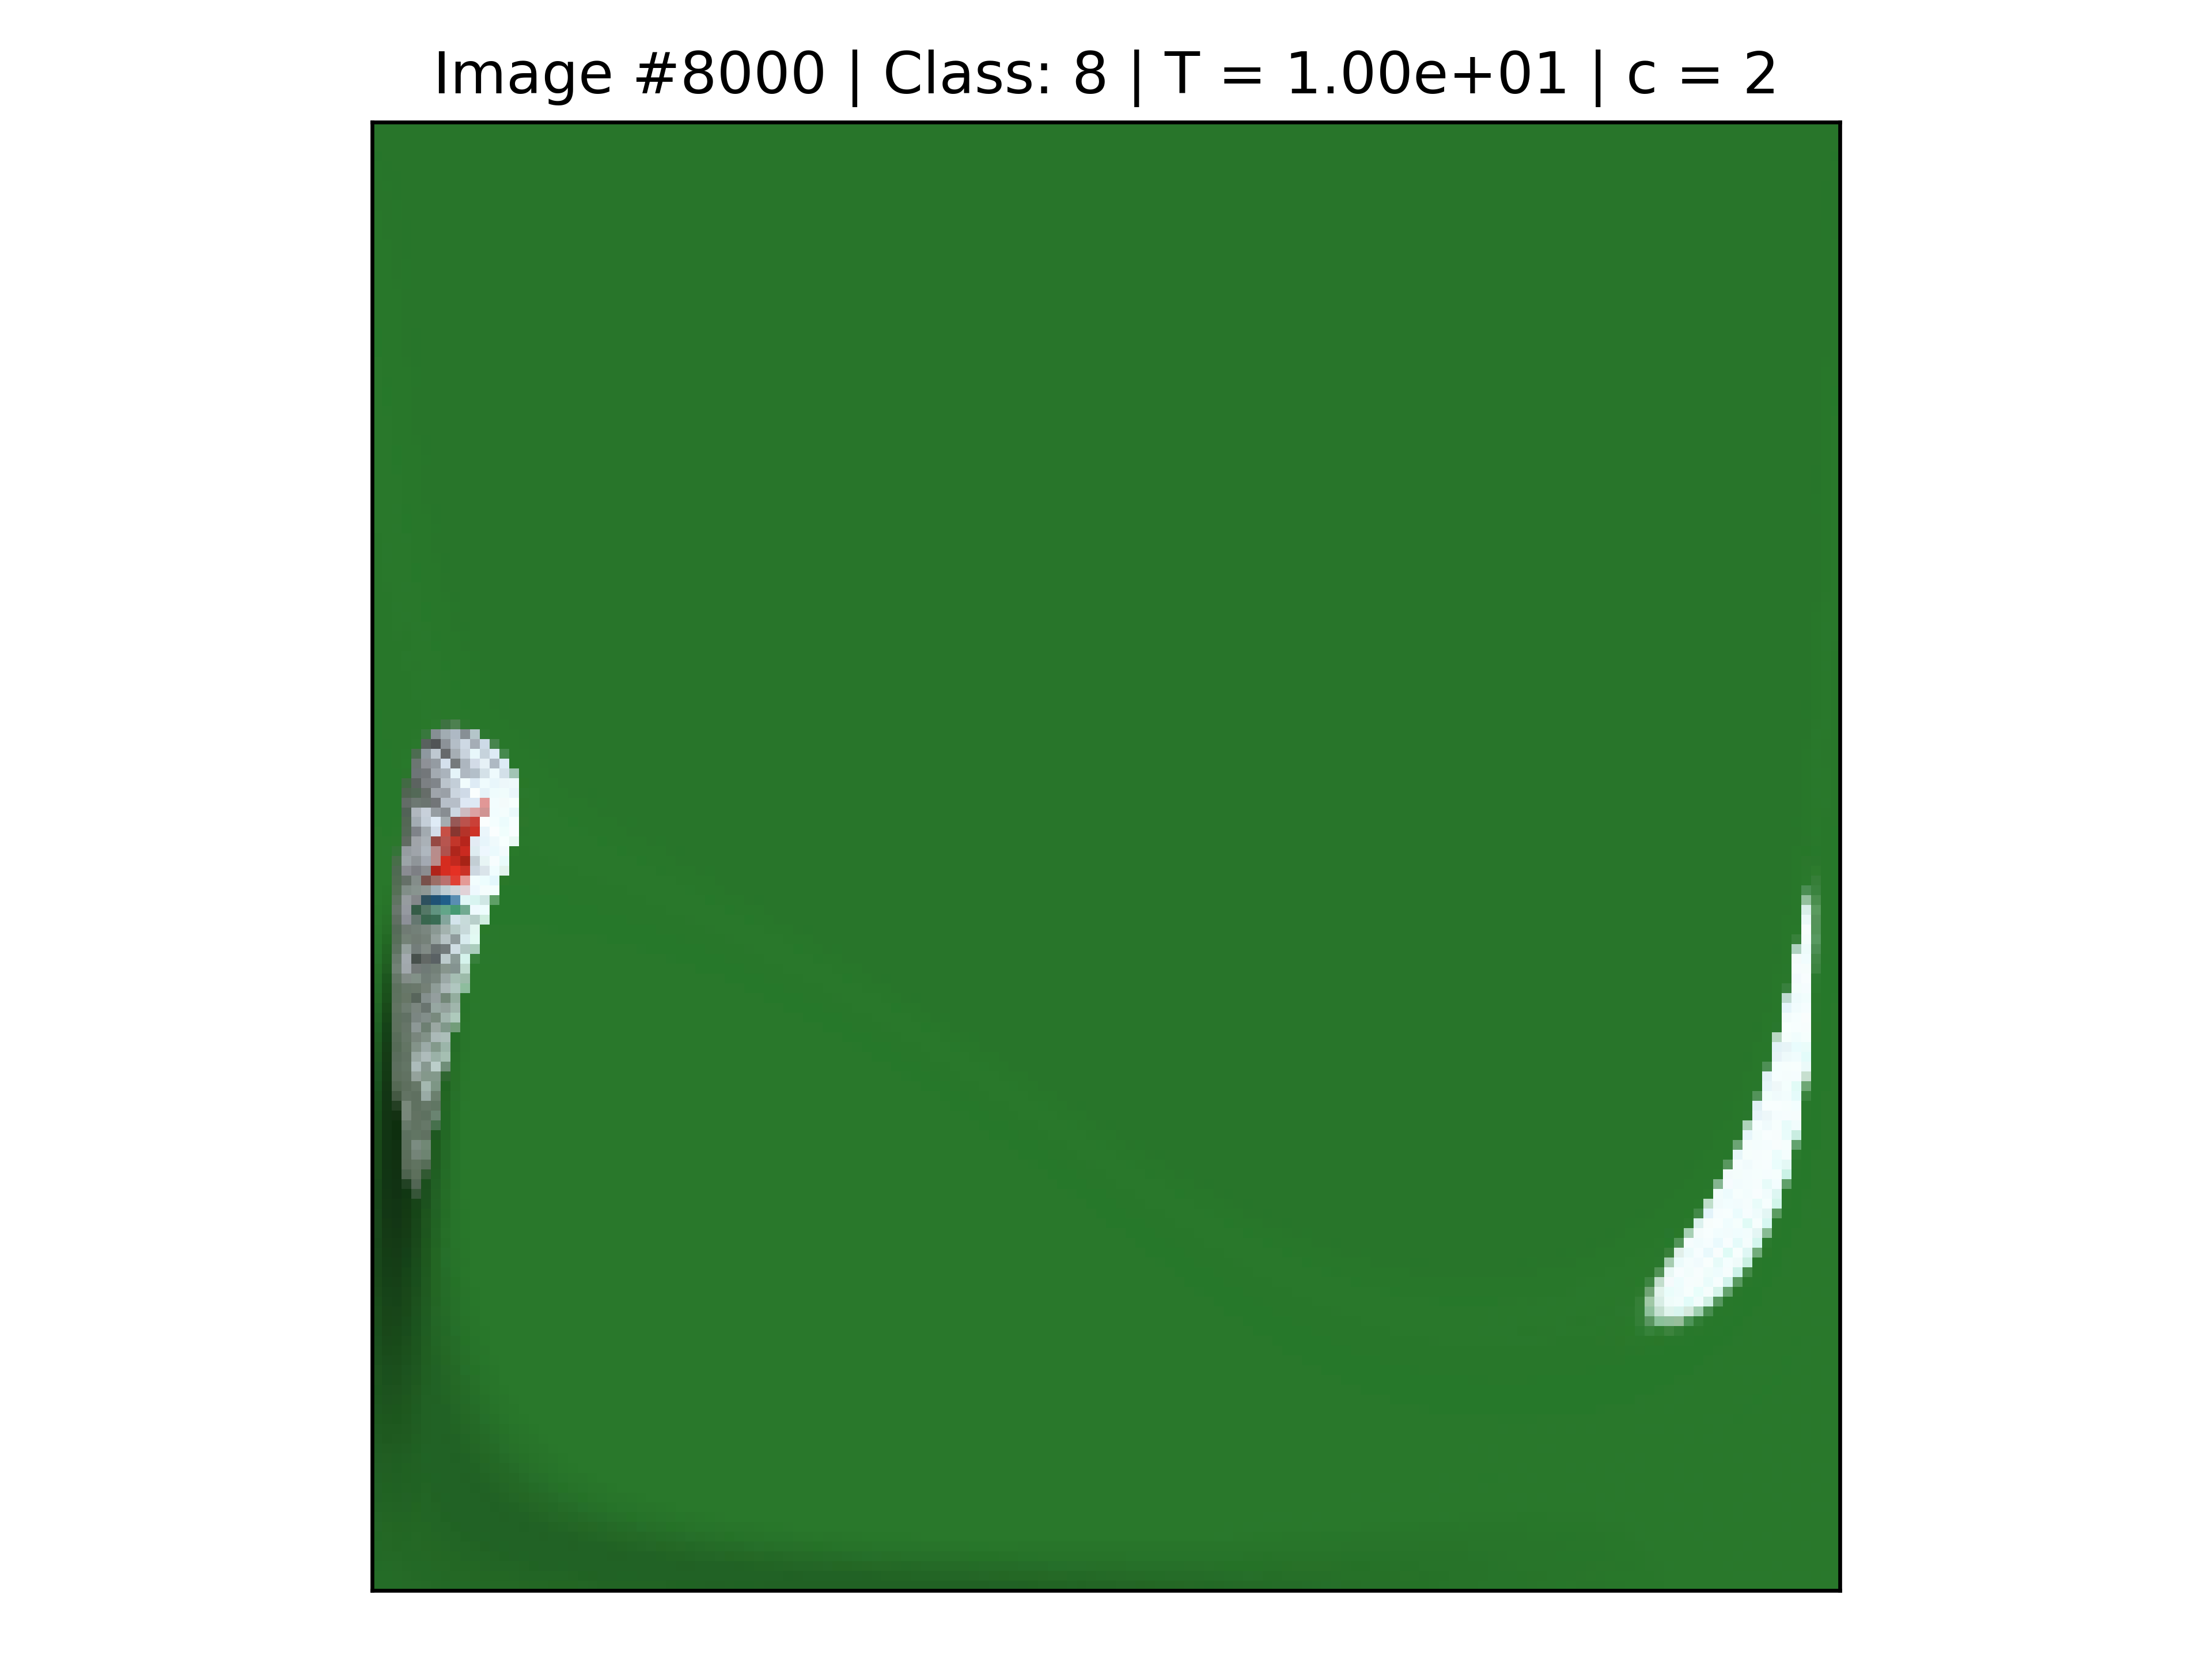
\includegraphics[width=\textwidth]{ch1-diffy/figures/warping_examples/8000_-1_2.png}
%    \caption{$T=10$}
%    % \label{fig:my_label}
%    \end{subfigure}
%    %%%%%
%    \centering
%    \begin{subfigure}{0.18\textwidth}
%    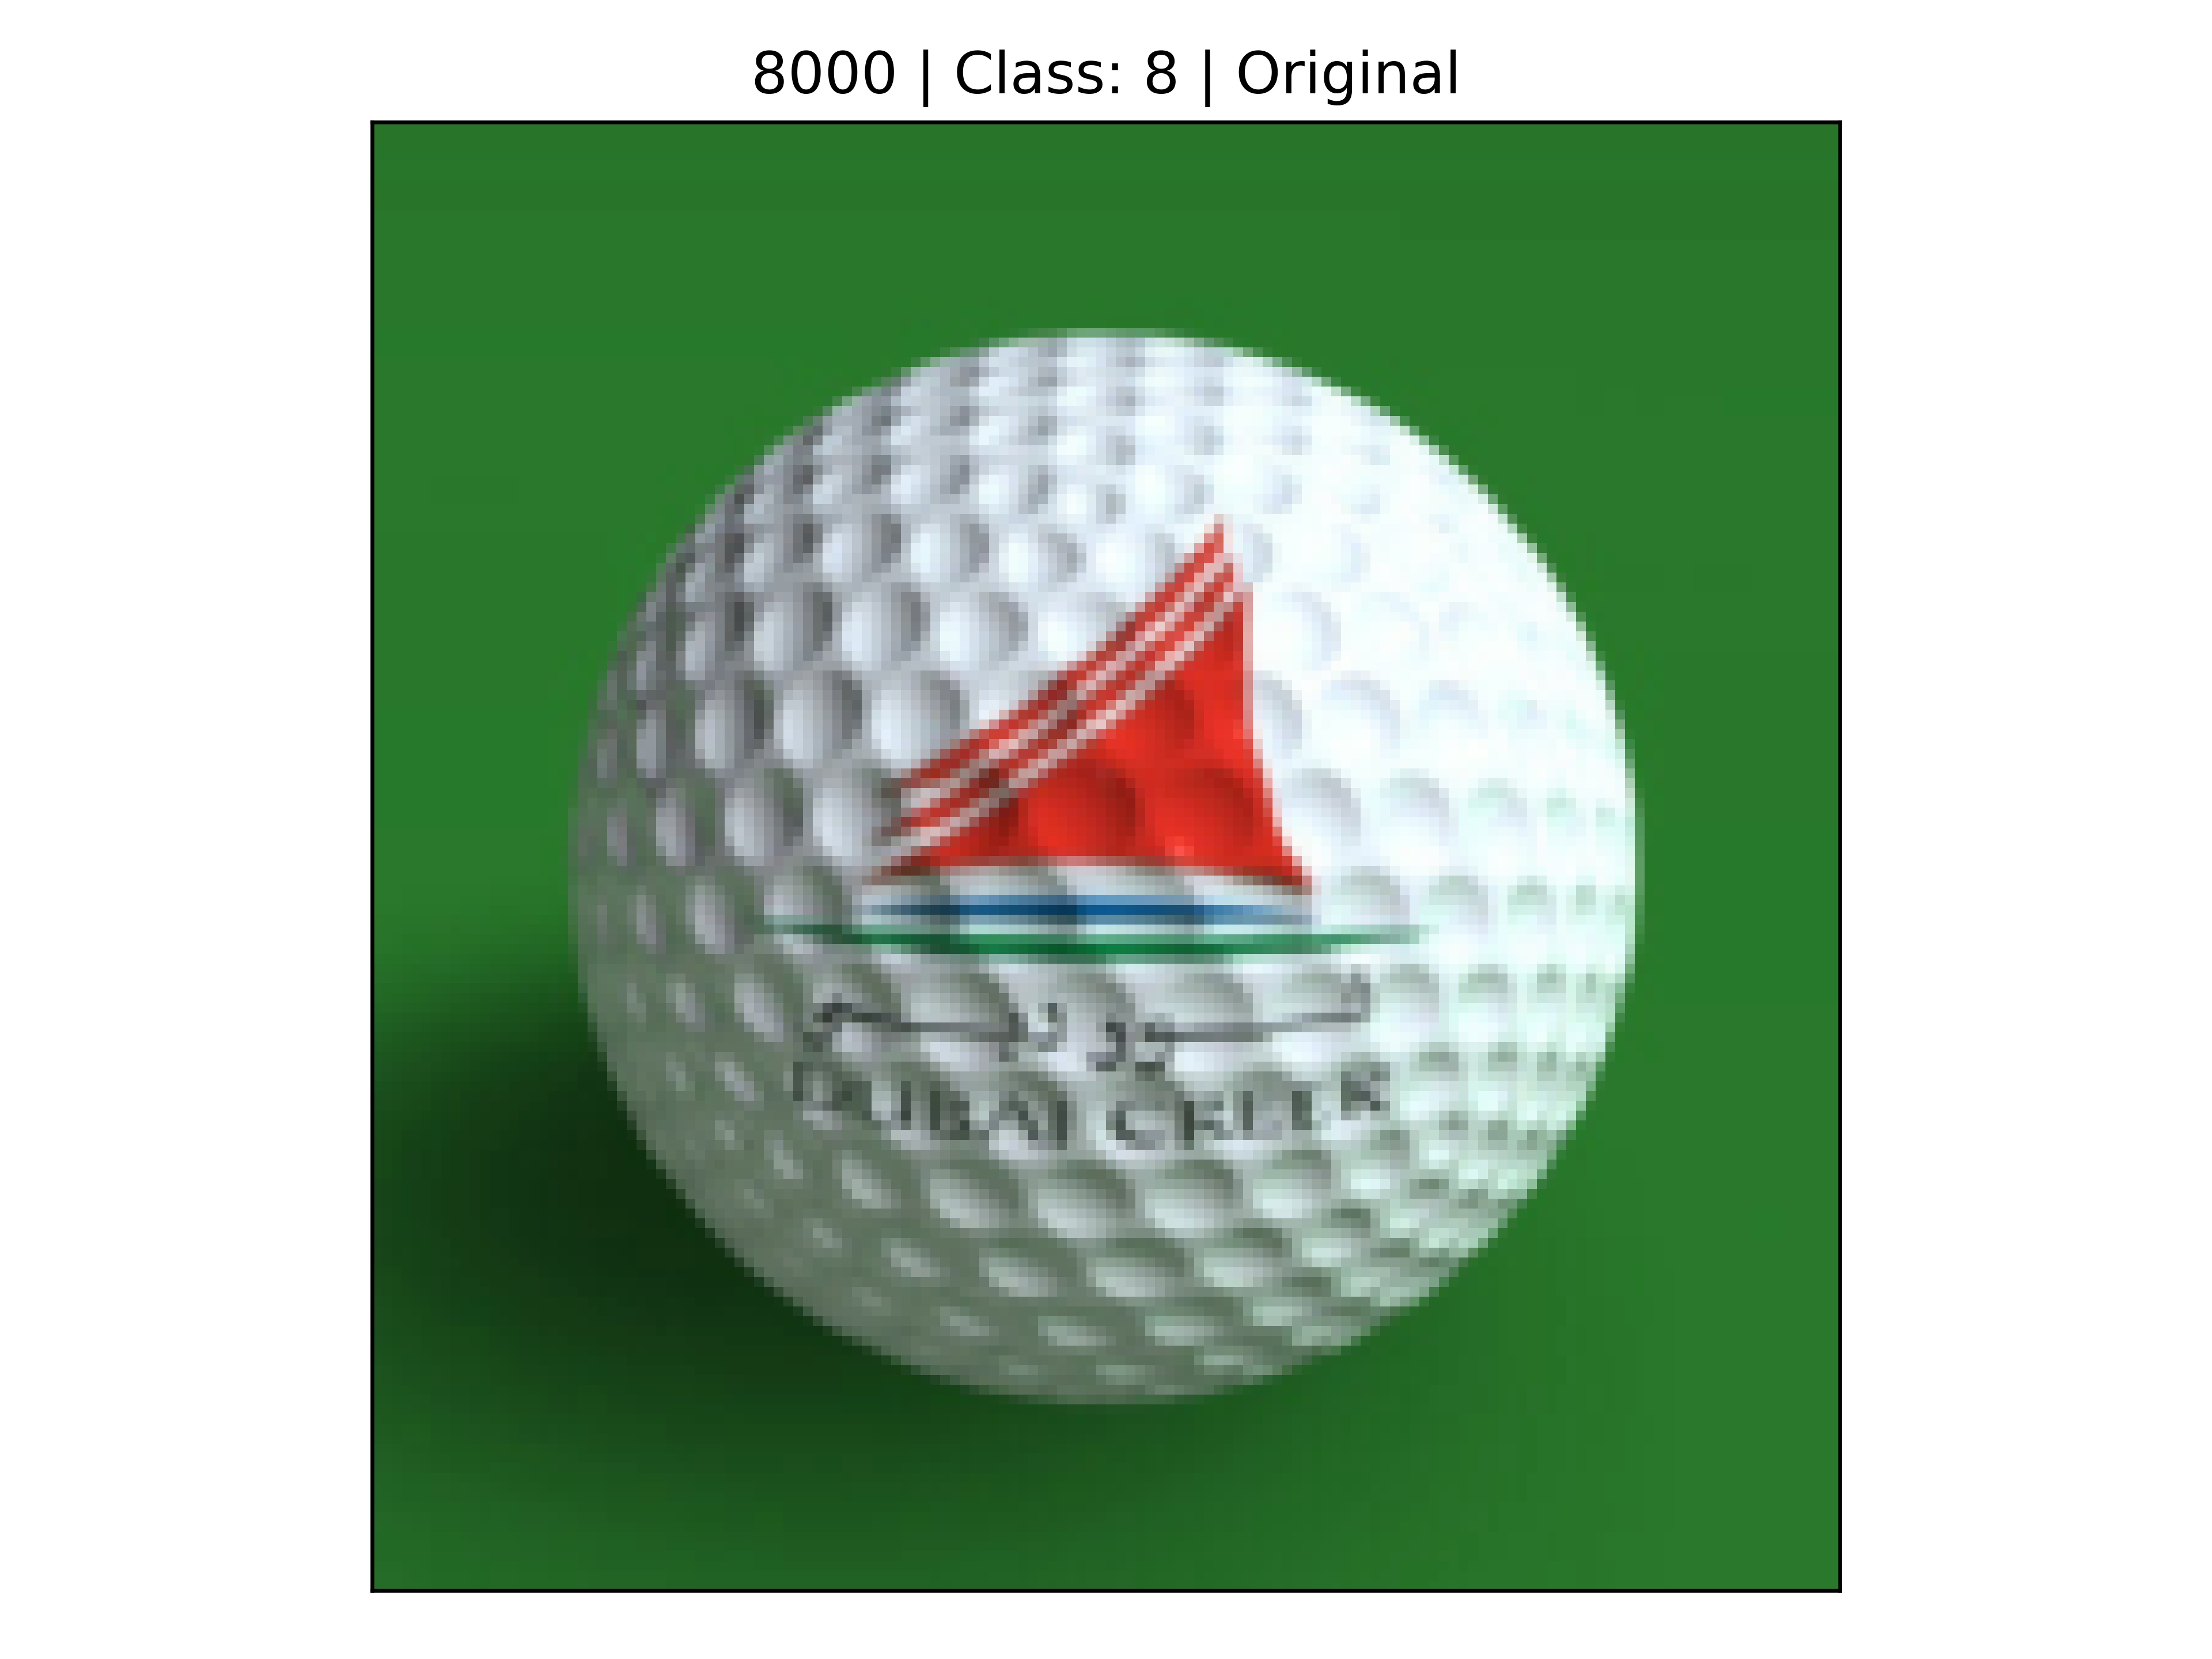
\includegraphics[width=\textwidth]{ch1-diffy/figures/warping_examples/8000.png}
%    \caption{Original}
%    % \label{fig:my_label}
%    \end{subfigure}
%    \caption{Image \#8000. Deformations $\text{warp}(f, T)$ for different values of $T$ ($c=2$).}
%\end{figure}

%\end{subappendices}

\chapter[DiffyTW: comparing time-series with smooth, time-warping invariance]{DiffyTW: comparing time-series with smooth, time-warping invariance}\label{ch:diffytw}
\chaptermark{DiffyTW}


\objectif{Measures of similarity (or dissimilarity) are a key ingredient to many machine learning algorithms. We introduce Diffy, a pairwise dissimilarity measure applicable to a wide range of data spaces, which leverages the data's internal structure to be invariant to diffeomorphisms. We prove that Diffy enjoys properties which make it relevant for theoretical study and practical use. By representing each datum as a function, Diffy is defined as the solution to an optimization problem in a Reproducing Kernel Hilbert Space and can be expressed in closed-form. In practice, it can be efficiently approximated via Nyström sampling. Empirical experiments support the merits of Diffy.}
\section{Introduction}

Time-series are ubiquitous in data analysis applications with tasks such as forecasting, classification or clustering and in fields such as medecine, atmospheric sciences and weather, finance and economics, or robotics.

At its heart, time-series analysis factors in the time-dependent structure of collected data\footnote{We will also study this problem for filtering in \cref{ch:hmm}.}. If this structure is to be exploited, time-series cannot be compared as if they were vectors in Euclidean space. Indeed, the points of two time-series do not necessarily portray data captured at comparable times (we say they are not \emph{aligned}). In fact, the instances can have a different number of points!

Dynamic Time Warping (DTW) was introduced by \cite{dtw-sakoe} to compare time series and account for misalignment. DTW became the \emph{de facto} standard for comparing time series in analysis tasks, as well as a strong baseline for classification when combined with the nearest neighbor classifier\cite{dtw-baseline-1, dtw-baseline-2}. Intuitively, Dynamic Time Warping finds a minimal-cost alignment between two time series, while respecting the order of the points. In practice refinements of the DTW are used that constrain the possible matchings\cite{dtw-baseline-1}. This minimization is carried out in $O(nm)$ where the compared time-series are of length $n$ and $m$. DTW does not take into account when the samples occur, only their relative order. DTW is differentiable with respect to one of its inputs as soon as there is a unique solution to the matching (that does not make the DTW zero). Non-differentiability can happen in innocuous situations as illustrated in \cite{tavenard-dtw-diff}. Despite being non-smooth, DTW-based averaging methods such as DBA have been proposed\cite{dba-petitjean}.

Soft Dynamic Time Warping (Soft-DTW) was proposed in \cite{sdtw} as a smooth replacement for DTW. Empirically, Soft-DTW behaves similarly to DTW, has equivalent computational complexity, is differentiable, and works better than DTW-based DBA for averaging based methods like clustering.

\paragraph{Related work}
While DTW and Soft-DTW are the most widely used elastic distances on time-series, other distances include: Fréchet distance \citep{frechet-clustering}, the Continuous-DTW distance\citep{cdtw}, extensions of (soft)DTW to comparing the feature space as well \citep{dtw-incomparable,vayer2022time}.

Functional data analysis methods have also been proposed, especiallly around the seminal contribution of the Square-Root Velocity representation\citep{srvf}. Another approach is to use the moments of a functions, depending on its higher-order derivatives\citep{0712.1425}. Shape analysis methods have also been applied to time-series of shapes\citep{2108.05634,hal-00813825}. Neural network methods including with neural networks that learn an alignment function from the dataset\citep{2106.11911,dtan,2206.08107}. These methods focus on the alignement task and do not develop dissimilarities between time-series.

\paragraph{Approach \& Contributions}
DiffyTW is divergence between functions on $[0,1]$ representing time-series. It is provably invariant to subset of smooth reparametrizations. The set of transformations it is invariant to can be tuned. It can be robustly and efficiently used to compare time-series, by solving a quadratic program. DiffyTW produces a dissimilarity score and a reparametrization that aligns the time series. DiffyTW is differentiable with respect to its input and can be integrated in wider machine learning workflows. We illustrate and study DiffyTW's behavior on time series empirically.

\paragraph{Notation} In this chapter, a time series is represented by a sample pattern $(t_i)_{1 \leq i \leq n}$ such that $0 = t_1 < \ldots < t_n = 1$ (not necessarily random) and values $(f_i)_{1\leq i\leq n}$ where $f_i \in\mathbb R^d$. $k$ is a positive definite kernel on $\mathbb R$ with reproducing kernel Hilbert space $\mathcal F$. $K$ is a positive definite kernel with reproducing kernel Hilbert space $\mathcal H$. Functions $f,g:[0,1] \to \mathcal X$, where $\mathcal X$ is a metric space, generally $\mathcal R^d$.

\section{DiffyTW}
In this section, we introduce DiffyTW, a divergence between functions $[0,1] \to \mathcal X$ which is invariant to a chosen class of diffeomorphic reparametrizations of $[0,1]$.

\subsection{Intuition}
We call \emph{reparametrization} any increasing, diffeomorphic function $Q:[0,1] \to [0,1]$. Let $\mathcal Q$ be a set of such functions. Our goal is to concieve a divergence such that $d(f\circ Q, f) = 0$ for any $Q\in\mathcal Q$ and any $f:[0,1] \to \mathbb R^d$.

A key idea is to compare the integrals of $f\circ Q$ and $f$. Indeed, this allows one to apply the change of variable theorem \citep{change-variable-ref}:
\begin{equation}
    \int_0^1 f\circ Q(x)Q^\prime(x)dx = \int_0^1 f(x)dx.
\end{equation}
The intuition is then that finding $q(x) = Q^\prime(x)$ makes the integrals match, and makes the difference between both integrals small. This was also proposed in \cref{ch:diffy} for handling invariances on general data spaces. We highlight differences with \ciref{ch:diffy} in \cref{sec:diffytw-vs-diffy}.

If $q = Q^\prime$ is contained in the space we optimized over,
\begin{equation}
    q \mapsto \left\vert\int_0^1 f\circ Q(x)q(x) dx - \int_0^1 f(x)dx\right\vert
\end{equation}
is minimized by $q=Q^\prime$. However, in general, we cannot exhaustively specify the set of transformations the problem is invariant to, and $q=Q^\prime$ may not be the only minimizer in the space. Indeed, if $f:[0,1] \to \mathbb R^+$, then $q(x) = f(x) / f\circ Q(x)$ also minimizes this quantity.

\paragraph{}
Such spurious minimizers can be avoided with two refinements.

First, to ensure matchings work for all features of the time series, we embed their values with $\phi$, chosen as a high-dimensional embedding. This avoids the minimizer above, but also handles the case where $f(x)\in\mathbb R^d$. Indeed, if the match is not perfect, then $f$ and $g$ can be made close by favoring the coordinates with the highest magnitude. This is avoided when embedding with $\phi$.

Second, we enforce the search space to contain only derivatives of reparametrizations, i.e. we restrict functions $q$ to verify the two following constraints: $q(x) \geq 0, \forall x\in[0,1]$ and $\int_0^1 q(u)du=1$. As a byproduct, retieving $q$ allows us to reconstruct a reparametrization $Q$ and align the time series.

\subsection{Definition of DiffyTW}

Let $\mathcal F$ be a space of functions $[0, 1] \to \mathbb R$. Let $\mathcal F_{0,1} \subset \mathcal F$ be a subset of $\mathcal F$ such that if $q\in\mathcal F_{0,1}$, $q\geq 0$ and $\int_0^1q(t)dt =1$. $\mathcal F_{0,1}$ defines the class of diffeormophic reparametrizations the divergence is invariant to through its derivatives. We denote $\mathcal Q$ the set of reparametrizations obtained by integrating the elements of $\mathcal F_{0,1}$, i.e.
\begin{equation}
    \mathcal Q = \left\lbrace Q: x\in[0,1] \mapsto \int_0^x q(x)dx ~\vert~ q \in \mathcal F_{0,1}\right\rbrace
\end{equation}

\begin{definition}[DiffyTW]\label{def:diffytw}
Let $d: \mathcal X^{[0,1]} \times \mathcal X^{[0,1]} \to \mathbb R^+$ be for any $f, g\in\mathcal X^{[0,1]}$,
\begin{equation}\label{eq:diffytw}
    d(f, g) = \min_{q \in \mathcal F_{0,1}}\left\Vert \int_0^1 \phi(f(x))q(x)dx - \int_0^1\phi(g(x))dx\right\Vert^2_\mathcal H.
\end{equation}
We call this divergence DiffyTW.
\end{definition}

Note that as soon as $f$ and $g$ and measurable, then $d$ is well defined. Indeed, since $\phi$ is bounded on $[0,1]$ and $q$ is integrable, the integrals are well-defined Bochner integrals and $d(f, g)$ is finite and well-defined.

\paragraph{Time-series alignment}
If $f$ and $g$ are two functions representing two time-series, DiffyTW aligns $f$ and $g$. Indeed, we can -- applying the change of variable theorem -- rewrite \cref{eq:diffytw} as
\begin{equation}\label{eq:diffytw-Q}
    d(f, g) = \min_{Q \in \mathcal Q} \left\Vert \int_0^1 \phi(f \circ Q^{-1}(x))dx - \int_0^1\phi(g(x))dx\right\Vert^2_\mathcal H
\end{equation}

\noindent \Cref{eq:diffytw-Q} shows we that the minimizer of the optimization problem in \cref{eq:diffytw} is the derivative of the reparametrization that aligns $f$ with $g$ in terms of the embedding $f \mapsto \int \phi(f(x))dx$.

We adopt the following notation for convenience:
\begin{equation}\label{def:diffytw-delta}
\Delta(f , g) = \left\Vert \int_0^1 \phi(f(x))dx - \int_0^1\phi(g(x))dx\right\Vert^2_\mathcal H
\end{equation}

\begin{figure}[ht!]
\begin{center}
\includegraphics[width=0.45\textwidth]{ch3-diffytw/figures/trace-demo.pdf}
\includegraphics[width=0.45\textwidth]{ch3-diffytw/figures/trace-demo-Q.pdf}
\end{center}
\caption[Time series alignment with DiffyTW]{Time series aligment with DiffyTW: in this example, time series $g$ is transformed into $f=g\circ Q$ by reparametrization $Q$. The reparametrization computed by DiffyTW is $\hat Q$, and reconstruction $\hat f$ of $f$, which agrees with $f$.\textsuperscript{*}}
\small\textsuperscript{*} Details: An instance $g$ of the Trace dataset from the UCR repository is transformed into $f$ by a reparametrization $Q$ induced by a NNLM from $\mathcal F_{0,1}^{M_w}$ with $M_{w}=30$ and $\eta_w= 100$ for the RBF kernel (see right plot, continous line). $\hat d_M$ is computed using parameters $M=100$, $\eta =100$ for the Laplace kernel (kernel $k$ that over time) and $\gamma=10$ for the RBF kernel (kernel $K$ over features). $\hat Q$ is the reconstruction of $Q$ from the solution to DiffyTW.
\end{figure}

\subsection{Invariance to time-warping}
DiffyTW was designed to be equal to zero when comparing functions that are diffeomorphic one to the other, i.e. $d(f\circ Q, f)=0$. We show this is \cref{thm:diffytw-invariance}:


\begin{theorem}\label{thm:diffytw-invariance}
Let $Q$ be a reparametrization of $[0,1]$ such that $Q^\prime \in \mathcal F_{0, 1}$. Then, for any $f: [0,1] \to \mathcal X$,
\begin{equation}
    d(f\circ Q, f) = 0.
\end{equation}
\end{theorem}

\begin{proof}
Let $f: [0,1] \to\mathbb R^d$ a measurable function. $Q:[0,1] \to [0,1]$ is continuously differentiable, bijective and $Q^{-1}$ is continuously differentiable. We apply the Change of variable theorem:
\begin{equation}
\int_0^1 \phi(f\circ Q(x))\vert Q^\prime(x)\vert dx = \int_0^1 \phi(f(x))dx.
\end{equation}

Since $Q$ is a reparametrization, it is increasing and $Q^\prime(x) \geq 0$ so we can drop the absolute value.

Since $Q^\prime \in \mathcal F_{0,1}$,
\begin{equation}
    d(f\circ Q, f) \leq \left \Vert \int_0^1 \phi(f\circ Q(x))Q^\prime(x)dx - \int_0^1 \phi(f(x))dx\right\Vert_\mathcal H^2
\end{equation}
and finally,
\begin{equation}
    d(f\circ Q, f) \leq 0.
\end{equation}
Since $d(f\circ Q, f) \geq 0$, we have proven the result.
\end{proof}


Of course, in practice, one wishes to compute $d(f, g)$ where $f$ and $g$ are not exactly diffeomorphic. In \cref{prop:diffytw-properties} we show that some intuitive invariance properties remain:
\begin{proposition}\label{prop:diffytw-properties} Let $f, g:[0,1] \to\mathbb R^d$. Then, $d$ verifies the following properties:
\begin{enumerate}
\item[(a)]if $id \in Q$, $d$ is a semi pseudo-distance, i.e. for any $f, g: [0,1] \to\mathcal X$,  $d(f, g)\geq 0$ and $d(f, f)=0$.
\item[(b)]if $id \in \mathcal Q$ and $Q_0\in\mathcal Q$ is such that $\Delta(f\circ Q_0^{-1}, g) \leq d(f, g) + \varepsilon$ then, $d(f \circ Q_0^{-1}, g) \leq d(f, g) + \varepsilon$. In particular, if $\Delta(f\circ Q_0^{-1}, g) = d(f,g)$ then $d(f\circ Q_0^{-1}, g)=d(f, g)$.
\item[(c)] if $Q_0$ is a reparametrization that leaves $\mathcal Q$ invariant (i.e. $\lbrace Q\circ Q_0 ~\vert~ Q\in \mathcal Q \rbrace = \mathcal Q$), then $d(f\circ Q_0^{-1}, g) = d(f, g)$.
\end{enumerate}
\end{proposition}
\begin{proof} (a) is clear. Proof of (b) follows from noticing that:
\begin{equation}
d(f\circ Q_0^{-1}) \leq \Delta(f\circ Q_0^{-1}, g)
\end{equation}
Finally, proof of (c) follows from noticing that:
\begin{align}
d(f \circ Q_0^{-1}, g) &= \min_{Q\in\mathcal Q}\Delta(f\circ Q_0^{-1} \circ Q^{-1}, g)\\
& = \min_{R\in\mathcal Q} \Delta(F\circ R^{-1}, g)\\
& = d(f, g),
\end{align} where the second equality comes from the change of variable $Q \to R \circ Q_0^{-1}$, which does not modify the set we optimize over by hypothesis.
\end{proof}

\section{Computing DiffyTW in practice}\label{sec:computing-diffytw}
DiffyTW is defined over the space of functions $[0,1] \to \mathcal X$ and the optimization problem is defined over an arbitrary set of functions $\mathcal F_{0,1}$, which determines the set of transformations $\mathcal Q$ the divergence is invariant to. In this section, we show DiffyTW can be computed for sampled time-series and with an expressive set of diffeomorphims $\mathcal F_{0,1}^M$ by solving a Quadratic program. We show that this approximate computation is exact if we assume the underlying signals are piece-wise constant. When the signals have regularity, we show that as the number of sample points grow, the approximated DiffyTW value approaches that compyuted on the underlying signals.

\emph{\textbf{In what follows, we highlight the main ingredients and steps in our reasoning.} Formal definitions of components, statements of results and proofs follow in the rest of the section and related appendices.}

\paragraph{Time-series as piece-wise constant functions} Times series are discrete objectifs, with data arriving at different time points. By representing them as piece-wise constant functions (i.e. step functions), we take into account the relative position between the sample points and their values. %Consider $f$ and $g$ two piece-wise constant functions adapted to $(x_1, \ldots, x_n)$ and $(y_1, \ldots, y_m)$. A piece-wise constant function is adapted to an increasing sequence of distinct points in its domain if $f$ is a constant between each point.
Thus we define $\hat f(\hat f, \hat g) =d(f, g)$ where $f$ and $g$ are piece-wise constant functions adapted to $\hat f$ and $\hat g$. By doing so, we can rewrite the integrals in the definition of \cref{eq:diffytw} as follows:
\begin{align}
    \hat d(\hat f, \hat g) &= \min_{q \in \mathcal F_{0,1}}\left\Vert \int_0^1 \phi(f(x))q(x)dx - \int_0^1\phi(g(x))dx\right\Vert^2_\mathcal H\label{eq:diffytw-step-1}\\
            &\label{eq:diffytw-step-2}= \min_{q\in\mathcal F_{0,1}} \left \Vert \sum_{i=1}^{n-1} \underbrace{\int_{x_i}^{x_{i+1}}q(u)du}_{I(q, x_i, x_{i+1})} \phi(f(x_i)) - \sum_{j=1}^{m-1} (y_{j+1} - y_j)\phi(g(y_j))\right\Vert_\mathcal H^2
            %&\label{eq:diffytw-step-3}=\min_{\substack{q\in\mathbb R^{M}\\h^\top q=1\\0 \leq q}}\frac{1}{2}q^\top Pq - v^\top q + C
\end{align}

\paragraph{Linear parametrization of $\mathcal F_{0,1}$} If $\mathcal F_{0,1}$ is chosen to be very general, then the optimization problem in \cref{eq:diffytw} is intractable. Furthermore, from a modelling perspective, very large diffeomorphism classes may encompass transformations that are not representative of the invariance structure present in data. We propose to choose $\mathcal F_{0,1}^M\subset \mathcal F_{0,1}$ such that solving \cref{eq:diffytw} is feasible and such that $\mathcal F_{0,1}^M$ is expressive enough to encompass a wide class of transformations. Anotherway of seeing things -- in the spirit of the approximation litterature -- is to consider how $\mathcal F_{0, 1}^M$ grows as $M \to \infty$.

In this chapter, we rely on Non-Negative Linear Models in the style of Gaussian Mixture Models of the form
\begin{equation}\label{eq:nnlm}
q(x) = \sum_{k=1}^M q_k k(x, \tilde x_k)\text{ such that } q_k\in\mathbb R^+, \int_0^1q(u)du=1
\end{equation}
%$q(x) = \sum_{k=1}^M q_k k(x, \tilde x_k)$ where $q_k$, $k$ and $\tilde x$ are chosen such that $q\in\mathcal F_{0,1}$.
For $q\in\mathcal F_{0,1}^M$, $I(q, x, y)$ can be computed in closed-form (see \cref{ex:H-rbf,ex:H-laplace}) and is linear in the coordinates $q$. This also implies that \cref{eq:nnlm} are linear equality and inequality constraints in $q$.

We define $d_M(f, g)$ as $d(f,g)$ replacing $\mathcal F_{0,1}$ by $\mathcal F_{0,1}^M$ in the optimization problem, i.e.:
\begin{equation}\label{eq:hat-d_M}
d_M(f, g) = \min_{q \in\mathcal F_{0,1}^M} \Vert \int \phi(f(x))q(x) - \int \phi(g(x))dx\Vert_\mathcal H^2
\end{equation}


\paragraph{Quadratric Program} We can now find a natural expression for $\hat d_M(\hat f, \hat g)$ which combines representing $\hat f$ and $\hat g$ by adapted piece-wise constant functions and optimizing over $\mathcal F_{0,1}^M$. We exploit the linearity in the coordinates on $q$ in \cref{eq:diffytw-step-2} and develop the squared-norm. This leads to defining $\hat d_M(\hat f, \hat g)$ as the optimal value to a Quadratic program over the coordinates $q$ with a single equality constraint (corresponding to $\int_0^1q(x)dx = 1$) and $M$ inequality constraints ($q \geq 0$):
\begin{equation}\label{eq:discrete-diffytw-informal}
\hat d_M(\hat f, \hat g) :=\min_{\substack{q\in\mathbb R^{M}\\h^\top q=1\\0 \leq q}}\frac{1}{2}q^\top Pq - v^\top q + C
\end{equation}
We define $\hat d_M(\hat f, \hat g)$ formally in \cref{sec:consistent}.

In the rest of \cref{sec:computing-diffytw}, we prove that \cref{eq:discrete-diffytw-informal} is consistent with \cref{def:diffytw}, that (under mild hypotheses) it is not sensitive to the sampling patterns of $\hat f$ and $\hat g$ as $n, m\to\infty$ and how it can be computed in practice.

%\subsection{Application to sampled time-series}

%A time series is a series of data points indexed in by time indexes. Often, the data points are taken at regular intervals. For instance, the position of a smartphone's GPS has a frequency around 1 Hz. However, this is not always the case. Indeed, in power-saving modes, a GPS position can be updated only when required by the algorithm or by the user.

%To incorporate the question of sampling pattern, we model a time series as n-tuple of couples $\left( t_i, f_i\right)_{1\leq i\leq n}$. The value $f_i$ is taken by the time-series at time $t_i$. We call $t_i$ sample points and the set $(t_i)_{1 \leq i \leq n}$ the sampling pattern. Without loss of generality, we assume that $0 \leq t_1 < \ldots < t_n \leq 1$.

%Given $\hat f_n = (t_i, f_i)_{1 \leq i\leq n}$ and $\hat g_m  = (s_j, g_j)_{1\leq j\leq m}$ taken from $f$ and $g$ we show that one can compute $d(\hat f_n, \hat g_m)$, by approximating $f$ and $g$ as rectangle functions. The approximated functions are denoted $\hat f_n$ and $\hat g_m$, by abuse of notation. We then show that $d(\hat f_n, \hat g_m)$ is close to $d(f, g)$ when $f,g$ have minimal regularity properties or if the sample pattern is random. For instance, if $f = g \circ Q$, then when $n, m \to 0$, $d(\hat f, \hat g) \to 0$.

%\subsection{Non-negative linear models}

%Non-negative linear models (NNLM) are widely used in probabilistic modeling, statistics and machine learning. One of the most well known classes are Gaussian Mixture Models (GMM).

%Let $M$ be a positive integer, the order of approximation considered. Let $(\tilde x_k)_{1\leq k\leq M}$ be $M$ distinct points in $[0, 1]$. To simplify our notations, we assume that $k < l \implies \tilde x_k < \tilde x_l$. We define the set of normalized NNLMs on $[0, 1]$ of order $M$ as the set of functions $q$ of the form
%\begin{equation}\label{eq:nnlm}
%q(x) = \sum_{k=1}^M q_k k(x, \tilde x_k)\text{ such that } q_k\in\mathbb R^+, \int_0^1q(u)du=1
%\end{equation}
%where $x \mapsto k(x, y)$ is a basis function, for instance the partial evaluation of a positive definite kernel. Normalized NNLMs are clearly a subset of $\mathcal F_{0,1}$, which we denote $\mathcal F_{0, 1}^M$. Note that $\mathcal F_{0,1}^M$ depends on the choice of kernel $k$ and of the set of anchor points $\tilde X = (\tilde x_k)_{1\leq k\leq M}$, both of which are fixed. When clear from context, we use the same notation for the function $q$ and the vector of coefficients $q\in{\mathbb R^+}^M$.


\subsection{Discrete DiffyTW is consistent with DiffyTW}\label{sec:consistent}
We begin by formally defining Discrete DiffyTW, as motivated above:
\begin{definition}[Discrete DiffyTW]\label{def:discrete-diffytw} Let $\hat f = (x_i, f_i)$ and $\hat g= (y_j, g_j)$. We define the discrete DiffyTW between discrete time series as the optimal value of the Quadratic program:
\begin{equation}\label{prob:qp}
    \hat d_M(\hat f, \hat g) :=\min_{\substack{q\in\mathbb R^{M}\\h^\top q=1\\0 \leq q}}\frac{1}{2}q^\top Pq - v^\top q + C
\end{equation}
where $P= 2\tilde H^\top K_{f, f}\tilde H$, $C= \delta^\top K_{g,g}\delta$ and $v= 2 \delta^\top K_{g,f}\tilde H$. $\delta\in\mathbb R^{m-1}$ is defined by $\delta_j = y_{j+1} - y_j$. $\tilde H$ is defined in \cref{eq:H}, $[K_{gf}]_{ij} = K(g_i, f_j)$, $[K_{ff}]_{ij} = K(f_i, f_j)$, and $[K_{gg}]_{ij} = K(g_i, g_j)$, where $K(z_1, z_2) = \langle \phi(z_1), \phi(z_2)\rangle_\mathcal H$.
\end{definition}
Notice that $P$ is symmetric, semi-definite positive by construction.

Our definition of $\hat d_M(\hat f, \hat g)$ coincides with that of DiffyTW when applied to piece-wise constant functions that interpolate $\hat f$ and $\hat g$ as defined in the \cref{thm:prob-qp} (for short, we say $f$ and $g$ are adapted to $\hat f$ and $\hat g$ respectively).

\begin{theorem}\label{thm:prob-qp}
Let $\hat f = (x_i, f_i)_{1 \leq i\leq n}$ and $\hat g = (y_j, g_j)_{1 \leq j\leq m}$ be two sampled time series. We define $f[0, 1]\to\mathbb R^d$ (resp. $g$) as the piece-wise constant function defined by $f([x_i, x_{i+1}[) = \lbrace f_i\rbrace$ (resp. $g([y_i, y_{j+1}[) = \lbrace g_j\rbrace$). Then:
\begin{equation}
d_M(f, g) = \hat d_M(\hat f, \hat g)
\end{equation}
where $d_M(f, g)$ is defined in \cref{eq:hat-d_M} and $\hat d_M(\hat f, \hat g)$ is defined in \cref{def:discrete-diffytw}.
\end{theorem}

The proof of \cref{thm:prob-qp} stems from the development at the beginning of \cref{sec:computing-diffytw} and can be found in \cref{proof:prob-qp}. A consequence of \cref{thm:prob-qp} is that some of the invariance properties of DiffyTW transfer to Discrete DiffyTW, i.e. Discrete DiffyTWequal to zero for discrete time-series which encode the time-warping of a piece-wise constant function:

\begin{corollary}\label{corollary:discrete-invariance}
Let $h: [0, 1] \to \mathbb R^d$ be a piece-wise constant function adapted to the sampling pattern $0 \leq x_1 < \ldots < x_n \leq 1$. Let $Q$ be a reparametrization such that $Q^\prime \in \mathcal F_{0,1}^M$. Consider $\hat f = (Q(x_i), h(x_i))$ and $\hat g = (x_i, h(x_i))$. Then,
\begin{equation}
    \hat d_M(\hat f, \hat g) = 0.
\end{equation}
\end{corollary}
The proof of \cref{corollary:discrete-invariance} can be found in \cref{proof:discrete-invariance}.

\subsection{Computing Discrete DiffyTW}\label{sec:solving-qp}

\Cref{prob:qp} is a quadratic program with $M$ variables and linear inequality and equality constraints. It is convex, and strongly convex as soon as $K_{f,f}$ is positive definite. The interior point Newton method, for instance in \cite{fabian} solves this type of convex problem. Their time complexity is generally in $O(M^3)$.

As a point of comparaison, Dynamic Time Warping can be computed in $O(M^2)$ time using Dynamic programming.

\subsection{Approximation error}
\cref{corollary:discrete-invariance} illustrates that the definition of Discrete DiffyTW is ``tight'' with respect to that of DiffyTW if the underlying signals are piece-wise constant and diffeomorphic. In this section, we raise three questions : how good is this approximation for arbitrary signals $f$ and $g$? how dependent is $\hat d_M(\hat f, \hat g)$ on the sampling patterns? how should one go about choosing $k$, $\tilde x$ and $K$?

\begin{theorem}[Rectangle approximation]\label{thm:rectangle-approx}
Let $f,g:[0,1] \to \mathbb R^d$ be two $L$-Lipchitz functions. Let $(x_i)_{1\leq i \leq n}$ and $(y_j)_{1\leq j\leq m}$ two sampling patterns. We denote $\hat f = (x_i, f(x_i))$ and $\hat g = (y_j, g(y_j))$.
If $K$ is the RBF kernel with $\gamma > 0$,
\begin{equation}
    \left\vert \sqrt{d_M(f, g)} - \sqrt{\hat d_M(\hat f_n, \hat g_m)}\right\vert \leq \sqrt{2\gamma L}\left(\sum_{i=1}^{n-1} (x_{i+1} - x_i)^{3/2} + \sum_{j=1}^{m-1} (y_{j+1} - y_j)^{3/2}\right)
\end{equation}

In particular, if $(x_i)$ and $(y_j)$ are evenly spaced in $[0,1]$, then:
\begin{equation}
    \left\vert \sqrt{d_M(f, g)} - \sqrt{\hat d_M(\hat f_n, \hat g_m)}\right\vert \leq \sqrt{2\gamma L}\left(\frac{1}{\sqrt{n}} - \frac{1}{\sqrt{m}}\right)
\end{equation}
\end{theorem}

\todo[inline]{Using $a^2- b^2 = (a-b)(a+b)$, restate on $d_m$ and $\hat d_M$}
\todo[inline]{Optimal rates ? This is with direct naïve proof.}

The proof on \cref{thm:rectangle-approx} is included in \cref{sec:proof-rectangle-approx}.

\subsection{Parameter choice}
Discrete DiffyTW has several hyper-parameters in particular the choice of $\mathcal F_{0,1}^M$ -- i.e. the basis function kernel $k(\cdot, \tilde x)$ and the anchor points $(\tilde x_k)_{1\leq j\leq M}$ -- and of $K$ the kernel on time-series features. When Discrete DiffyTW is integrated into a machine learning algorithm, a solution is to typical hyperparameter tuning strategies such as cross-validation. Below, we give intuition into the impact of the different hyperparameters.

The choice of basis function and the number and positions of the anchor points control the richness of the set of transformations that can be identified in data. The parameters of $k$ as well as $M$ should be chosen as a function of prior knowledge about the transformations present. For $k$ the RBF or Laplce kernel of parameter $\eta>0$, smaller values of $\eta$ and larger values of $M$ lead to richer function spaces. In addition, choosing the Laplace kernel makes for a much richer space than choosing the RBF kernel. Generally, $M$ is chosen to be much smaller than $n$ and $m$. Note that a richer space is not necessarily the goal as ``simple'' reparametrizations may make the most sense for an application.

The choice of kernel on time-series features has no impact on invariance for DiffyTW. However, empirically, we observe that it plays a role with Discrete DiffyTW. This is confirmed in \cref{thm:rectangle-approx} as $\gamma$, the RBF kernel parameter intervenes controls the value of the bound. Large values of $\gamma$ lead to larger values of the bound. Intuitively, this is explained by the fact that large values of $\gamma$ lead to a very discriminative kernel $K$. Loosely, any two distinct points seem very different. This implies having a large number of samples, in order to have sufficient overlap between the time-series (in $d$ this overlap is built-in as the functions are defined over $[0,1]$). On the other hand, a smaller $\gamma$ leads to a smaller bound, which means that $d$ and $\hat d_M$ are close. A small value for $\gamma$ means that $K$ is not very discriminative and any two values seem close. This applies to both $d$ and $\hat d_M$. In other words, $d$ (and $\hat d_M$) will be small for both pairs of diffeomorphic time-series and non-diffeomorphic time-series.

\section{Differentiability}
Differentiability makes Discrete DiffyTW effective as a building block inside of machine learning algorithms, for example as a loss function for training time-series generation algorithms.

We consider differentiability of $V(\theta) = \hat d_M(\hat f, \theta)$ and our goal is to compute $\nabla V(\theta)$, the gradient of $V$ with respect to $\theta$. Here, $\theta$ takes the place of $\hat g$ but we consider its sample pattern fixed. Additionally, $\nabla V(\theta)$ can be chained to extend to the (more common) case where we wish to compare $\hat f$ to $\hat g(\theta)$, a time-series generated by a model.

In this section, we denote:
\begin{equation}\label{prob:fullqp}
    V(\theta) = \min_{q\in\mathcal C} \ell(q, \theta)
\end{equation}
where $\ell(q, \theta) = \frac{1}{2} q^\top Pq - v(\theta)^\top q + C(\theta)$ and $\mathcal C = \left\lbrace q\in\mathbb R^N ~\vert~ h^\top q=1, q \geq 0\right\rbrace$.

The difficulty is differentiating through the $\min$ operator since the optimal $q^*$ depends on $\theta$. $V$ is differentiable and its gradient can be computed from the optimal solution $q^*$. Our proof is direct and does not rely on the Implicit Function Theorem (see below for a comparaison with other approaches).

\begin{theorem}\label{thm:diffytw-grad}
    If $\ell(\cdot, \theta)$ is strictly convex, then $V(\theta)$ is differentiable and
    \begin{equation}
        \nabla V(\theta) = J_\theta \ell(q^*(\theta), \theta) + \nabla C(\theta),
    \end{equation} where $q^*(\theta)$ is the unique solution to \cref{prob:fullqp}.
\end{theorem}

In particular, so long as $P$ is positive definite, $V$ is differentiable. This is ensured in all practical situations by definition of the Discrete DiffyTW. In practice, regularization is added to $P$ under the form $P + \lambda I$ to make the Quadratic program solver more stable.

Our proof of \cref{thm:diffytw-grad} builds on a result from \cite{shapiro} and \cite{lee}, which give sufficient conditions for differentiability of quadratic programs. See \cref{sec:proof-diffytw-grad} for the proof. Note that a similar argument is used in \cite{tavenard-dtw-diff} for the differentiability of DTW.

\paragraph{Other methods for differentiability of QPs}
There is a growing body of work on differentiating through convex programs, with three major approaches: analytical differentiation (when a closed-form solution to the convex problem is known, \emph{e.g.\ } unconstrained QPs), unrolling (differentiating through the operations in the algorithm used to solve the convex problem), implicit differentiation (applying the implicit function theorem).

\begin{remark}[Relation to implicit differentiation for QPs]
    \cite{bambade,optnet,...} study differentiation of Quadratic programs where the constraints also depend on $\theta$. They rely on implicit differentiation of the KKT conditions for the Quadratic Program and handle a more general setting, including Extended Conservative Jacobians when the QPs are not feasible. As a sanity check, we verify that we recover our result using their method for our setting in \cref{sec:lagrangian}.
\end{remark}

\section{Experiments}
DiffyTW is implemented in the \texttt{difftw} library, open-sourced at \url{github.com/theophilec/diffytw}. This library implements the computation of DiffyTW, the gradient computation using the \texttt{jax} library. It can be used with different QP solvers.

In this section, we demonstrate and study DiffyTW's behavior on the UCR dataset. Some takeaways of these experiments are:

\begin{itemize}
    \item DiffyTW captures synthetic diffeomorphisms.
    \item DiffyTW is sensitive to the choice of $\gamma$ (and more generally to the choice of $\phi$), including with synthetic warpings. Making DiffyTW more robust to this choice is key to making it useful for applied settings (such as averaging), and this is left for future work.
    \item Regularizing the choice of $q$ has significant effect on the robustness of DiffyTW. Regularization is not studied in the previous sections and it is incorporated in practice by padding the Hessian matrix, which is necessary for numerical reasons. Adding regularization to the definition of DiffyTW (in the spirit of Diffy in \cref{ch:diffy}) and analyzing its role is left for future work.
\end{itemize}

\subsection{Introduction}

\paragraph{Experiment design}
We choose $\tilde X = (\tilde x_k)_{1\leq k \leq M}$ anchor points, $\eta >0$ and choose $\mathcal F_{0,1}^M$ to be the set of functions of the form $q(x) = \sum_{k=1}^Mq_k k_\eta(x, \tilde x_k)$ where $q\in\mathbb R^M$ verifies: $q \geq 0$, $g^\top q =1$, and $\int_0^1 q(u)du =1$.
We consider $K$ the RBF kernel with $\gamma> 0$.

\paragraph{Datasets} We rely on the UCR dataset\cite{ucr}. Specifically we use the Trace dataset. We compare elements of datasets, but also synthetic transformations of times-series from the UCR dataset. In that case, we consider the linear interpolation of $g \circ Q$. For completeness here is the Python code used for a time-series $x, g$ and a warping function $Q$: \texttt{np.interp(Q(x), x, g)}. Since these time series are well-sampled, we ignore the errors caused by interpolation.



\subsection{Alignment with synthetic warpings} \emph{In this section, we illustrate the behavior of DiffyTW on a real dataset with synthetic warpings. This ensures that the warpings are attainable by DiffyTW.}

Here we choose $\hat g\in\mathcal S$ (for Trace), generate $q \in \mathcal F_{0, 1}^M$ and $\hat f$ the transformation of $g$ by $Q = \int q$ (according to linear interpolation). We then compute $\hat d_M(\hat f, \hat g)$ over the same space $\mathcal F_{0,1}^M$ (we call this setting ``in-domain''). The value of $\eta$ is fixed by $\mathcal F^M$ but we show results with the best value of $\gamma$. We study the dependence on $\gamma$ in \cref{sec:XP-gamma}.










\subsection{Dependence of $\gamma$}\label{sec:XP-gamma}

\begin{figure}[ht!]
\begin{center}
\includegraphics[width=\textwidth]{ch3-diffytw/figures/Figure-50words-rbf-30_rbf-100-laplace-10000.0-100-1.0e-05.pdf}
\end{center}
\caption[itopto]{Sensitivity to choice of $\gamma$}
\small\textsuperscript{*} Details: For computing DiffyTW between the original and transformed time-series, the RBF kernel with parameter $\eta=100.0$ and $M=100$ anchor points is used for the time space, and the Laplace kernel with varying parameter $\gamma$.
\end{figure}

\begin{figure}[ht!]
\centering
\includegraphics[width=0.8\textwidth]{ch3-diffytw/figures/Figure-outkernel-parameters.pdf}
\caption[Sensitivity of DiffyTW to the choice of $\gamma$.]{\textbf{Sensitivity to the choice of $\gamma$.} This graph shows the residual Euclidean error after alignment by DiffyTW: $\Vert f\circ Q - f\Vert_2\circ \hat Q$ where $Q(x) = \int_0^x q(u)du$ where $q$ is drawn from $\mathcal F_{0,1}^M$ and $\hat Q(x) = \int_0^x \hat q(u)du$ where $\hat q$ is the solution to Discrete DiffyTW over $\mathcal F_{0,1}^M$.}
\end{figure}

\begin{figure}[ht!]
\centering
\includegraphics[width=0.8\textwidth]{ch3-diffytw/figures/Figure-qnorm-qhatnorm.pdf}
\caption{}
\end{figure}


\subsection{Runtime speed}

\begin{subappendices}
\section{Quadrature of non-negative linear models}\label{app:diffytw-quadrature}

Given $q\in\mathcal F_{0,1}^M$, we introduce . $q\in{\mathbb R_{\geq 0}}^M \mapsto I(q, x, y)$ is linear in the coefficients.

Consider a fixed set of points $X=(x_i)_{1\leq i\leq n-1}$. We introduce
\begin{equation}
H: q\in\mathbb R_{\geq 0}^M \mapsto (I(q, x_i, x_{i+1}))_{1\leq i\leq n-1}\in \mathbb R^{N-1}
\end{equation}

$H$ is a linear map and we can represent it by a matrix in $\mathbb R^{N-1 \times M}$ such that if $q\in \mathcal F_{0,1}^M$, then $[Hq]_{i} = \int_{x_i}^{x_{i+1}}q(u)du$. Similarly, the map $q \mapsto \int_0^1 q(u)du$ is a linear form, linear in the coefficients $q$ and can be represented by an adjoint vector $h\in\mathbb R^M$.

$H$ and $h$ are given as a function of the basis function and the anchor points. For $1 \leq i \leq n-1$ and $1\leq k\leq M$,
\begin{align}\label{eq:H}
    H_{ik}= \int_{x_i}^{x_{i+1}}k(u, \tilde x_k)du&& h_k = \int_0^1 k(u, \tilde x_k)du
\end{align}

We derive the exact expressions in three cases in the following examples.

\begin{example}[RBF kernel]\label{ex:H-rbf} If $k$ is the RBF kernel with parameter $\eta > 0$, i.e. $k(x, y) = \exp\left( - \eta (x - y)^2\right)$, then
\begin{align}
    H_{i,k} &= \frac{1}{2}\sqrt{\frac{\pi}{\eta}}\left[\mathrm{erf}(\sqrt{\eta}(x_{i+1}-\tilde x_k) - \mathrm{erf}(\sqrt{\eta}(x_i- \tilde x_k) \right]\\
    h_k &= \frac{1}{2}\sqrt{\frac{\pi}{\eta}}\left[\mathrm{erf}(\sqrt{\eta}(1-\tilde x_k) - \mathrm{erf}(\sqrt{\eta}(- \tilde x_k) \right]
\end{align}
\end{example}
\begin{example}[Laplace kernel]\label{ex:H-laplace} If $k$ is the Laplace kernel with parameter $\gamma > 0$,i.e. $k(x, y) = \exp\left( - \gamma\vert x - y\vert\right)$, then
\begin{align}
    H_{i,k} &= \varphi(\gamma(x_{i+1} - \tilde x_k)) - \varphi(\gamma(x_i - \tilde x_k))\\
    h_{k} &= \varphi(\gamma(1- \tilde x_k)) - \varphi(\gamma(- \tilde x_k))
\end{align}
where $\varphi(u) = (2 - e^u)/\gamma$ if $u \geq 0$ and $\varphi(u) = e^{-u} / \gamma$ else.
\end{example}




\section{Proof of consistency}\label{proof:prob-qp}
\begin{proof}
Our goal is to prove that our definition of $\hat d_M(\hat f, \hat g)$ coincides with that of DiffyTW when applied to piece-wise constant functions that interpolate $\hat f$ and $\hat g$.

\subparagraph{Encoding the function space} $\mathcal F_{0, 1}^M$ is the set of functions parametrized by $q\in\mathbb R^M$ such that $q(x) \geq 0, \forall x\in [0,1]$ and $\int_0^1 q(x)dx= 1$. Let $h\in\mathbb R^M$ be such that $\int_0^1q(x)dx = h^\top q$. Then, the constraint $q\in\mathcal F_{0,1}^M$ can be replaced by $q\in\mathbb R^M$, $q\geq 0$ (coordinate-wise) and $h^\top q = 1$.


\subparagraph{Computing $d_M(f, g)$} Using the fact that $K(z_1, z_2) = \langle \phi(z_1), \phi(z_2)\rangle$ and $I(q, x_i, x_{i+1}) = [Hq]_i$, for any $q\in\mathcal F_{0,1}^M$,
\begin{align}
\left \Vert \int_0^1 \phi(f(x))q(x)dx \right\Vert^2_\mathcal H&=\left\Vert\sum_{i=1}^{n-1} \underbrace{\int_{x_i}^{x_{i+1}}q(u)du}_{I(q, x_i, x_{i+1})}\phi(f(x_i))\right\Vert_\mathcal H^2\\
&=\sum_{i=1}^{n-1}\sum_{j=1}^{n-1}\underbrace{I(q, x_i, x_{i+1})}_{[Hq]_i}I(q, x_j, x_{j+1})\underbrace{\langle \phi(f(x_i)), f(x_j))\rangle}_{K(f(x_i), f(x_j))}\\
&= q^\top H^\top K_{ff} H q
\end{align}

\begin{align}
\left\Vert\int_0^1\phi(g(x))dx\right\Vert_\mathcal H^2 &= \left\Vert\sum_{j=1}^{m-1} \underbrace{(y_{j+1} - y_j)}_{\delta_j}\phi(g(y_j))\right\Vert_\mathcal H^2\\
&= \sum_{j=1}^{m-1} \sum_{i=1}^{m-1} \delta_i \delta_j K(g(y_j), g(y_i))\\
& = \delta^\top K_{gg} \delta
\end{align}

\begin{align}
\left\langle \int\phi(f(x))q(x)dx, \int\phi(g(x))\right\rangle&=\sum_{i=1}^{n-1}\sum_{j=1}^{m-1} I(q, x_i, x_{i+1}) \delta_j \langle \phi(f(x_i)), \phi(g(x_j))\rangle\\
&= \delta^\top K_{gf} Hq
\end{align}

Thus by developing the squared-norm in the definition of $d_M(f, g)$,
\begin{equation}
d_M(f, g) = \min_{\substack{q\in\mathbb R^M \\ h^\top q = 1 \\ q \geq 0}} \frac{1}{2} q^\top P q - v^\top q + C
\end{equation}
where $P = 2 H^\top K_{ff}H$, $C = \delta^\top K_{gg}\delta$ and $v = 2\delta^\top K_{gf}H$, and we recover the definition of $\hat d_M(\hat f, \hat g)$.
\end{proof}

\section{Proof of the approximation theorem}\label{sec:proof-rectangle-approx}
\begin{lemma}\label{lemma:rectangle-approx}
Consider $f, g:[0, 1] \to \mathbb R^d$ and $s, r:[0,1] \to[0,1]$ two piece-wise constant functions such that $s(0)=r(0)=0$ and $s(1)=r(1)=1$. Then,
\begin{equation}
    \vert d(f, g) - d(f \circ s, g\circ r) \vert \leq \max_{q\in\mathcal F_{0,1}}\max_{x\in[0,1]}\vert q(x) \vert \left\Vert \int \phi(f) - \phi(f\circ s)\right\Vert_{\mathcal H} + \left\Vert \int \phi(g)- \phi(g\circ s)\right\Vert_\mathcal H
\end{equation}

\end{lemma}
\begin{proof}[Proof of \cref{lemma:rectangle-approx}]
Indeed, let $q\in\mathcal F_{0,1}$. By the triangle inequality,
\begin{align}
\left\Vert \int \phi(f(x))q(x)dx - \int \phi(g(x))dx \right\Vert
\leq
\left\Vert \int \phi(f(x))q(x)dx - \int \phi(f\circ s(x))q(x)dx \right\Vert\\
+ \left\Vert \int \phi(f\circ s(x))q(x)dx - \int \phi(g\circ r(x))dx \right\Vert
+ \left\Vert \int \phi(g\circ r(x))dx - \int \phi(g(x))dx \right\Vert
\end{align}
\end{proof}

\begin{lemma}\label{lemma:rbf-lip}
Let $\phi:\mathbb R^d \to \mathcal H$ such that $\langle
\phi(x), \phi(y)\rangle_\mathcal H = K(x, y)$ where $K$ is the RBF kernel with parameter $\gamma > 0$. Then,

\begin{equation}
\left\Vert \phi(z) - \phi(u)\right\Vert_\mathcal H \leq C_\gamma\sqrt{\Vert z - u \Vert_2}
\end{equation}
where $C_\gamma = \sqrt{\frac{2\sqrt{2\gamma}}{\sqrt{e}}}$.
\end{lemma}

\begin{proof}[Proof of \cref{lemma:rbf-lip}]

\begin{align}
\Vert \phi(z) - \phi(u)\Vert_\mathcal H^2 &= \Vert \phi(z) \Vert^2+ \Vert \phi(u)\Vert^2 - 2 \langle \phi(z), \phi(u)\rangle\\
&= 2 \left(1 - K(u, z)\right)
\end{align}

Denote $\varphi(x) = 1- e^{-\gamma x^2}$. $\varphi^\prime$ attains its global maxima at $x = \pm \sqrt{\frac{1}{2\gamma}}$, with value $\Vert \phi^\prime\Vert_{\infty} = \sqrt{\frac{2\gamma}{e}}$. And so:

\begin{align}
\Vert \phi(z) - \phi(u)\Vert_\mathcal H^2 & \leq \frac{2\sqrt{2\gamma}}{\sqrt{e}}\Vert z - u \Vert_2
\end{align}
\end{proof}

\begin{proof}[Proof of \cref{thm:rectangle-approx}]
Let $s:[0,1] \to [0,1]$ be a step function such that $f\circ s$ is adapted to $\hat f$. Similarly, let $r:[0,1]\to[0,1]$ be such that $g\circ r$ is adapted to $\hat g$. Then, by \cref{lemma:rectangle-approx},
\begin{equation}
    \vert d(f, g) - d(f \circ s, g\circ r) \vert \leq \max_{q\in\mathcal F_{0,1}}\Vert q \Vert_\mathcal H \left\Vert \int \phi(f) - \phi(f\circ s)\right\Vert_{\mathcal H} + \left\Vert \int \phi(g)- \phi(g\circ s)\right\Vert_\mathcal H
\end{equation}
By \cref{lemma:rbf-lip},
\begin{equation}
\left\Vert \int \phi(f) - \phi(f\circ s)\right\Vert_{\mathcal H} \leq \sum_{i=1}^{n-1} \delta_i^{3/2}C_\gamma\sqrt{\gamma L}
\end{equation}





Let $f$ be $L$-Lipschitz on $[0,1]$ and $\phi$ be the RBF kernel with parameter $\gamma > 0$.
Then, for any $\vert x - u \vert \leq \Delta$,
\begin{equation}
    \Vert \phi(f(x)) - \phi(f(u)) \Vert^2 \leq 2\left(1 - k(f(x), f(u))\right) \leq 2 \gamma L \Delta
\end{equation}
\end{proof}

\section{On the differentiability of DiffyTW}


\subsection{Proof of differentiality for DiffyTW}\label{sec:proof-diffytw-grad}
\begin{proof}

The set of admissible solutions $\mathcal C$ is non empty and is closed. Indeed, $\mathcal C$ is the intersection of a hyperplane ($h^\top q=1$) and of the non-negative quadrant ($q \geq 0$) ; both are closed so $\mathcal C$ is too.

Recall that $\ell(q, \theta) = \frac{1}{2}q^\top P(\theta) q - v(\theta)^\top q + C(\theta)$ where $\theta \mapsto P(\theta), \theta \mapsto v(\theta), \theta \mapsto C(\theta)$ are $\mathcal C^\infty$.

Our goal is to show that for any $\theta_0\in U :=\mathbb R^{n \times d}$, if $\bar q$ is the (unique) solution to quadratic program $\min_{q\in\mathcal C}\ell(q, \theta)$, which we denote as $\mathcal P(\theta_0)$ , then
   \begin{equation}\label{eq:goal}
       V(\theta_0 + d) - V(\theta_0) = D_\theta \ell(\bar q, \theta)d + o\left(\Vert d\Vert\right)
   \end{equation}
   where $D_q \ell$ is the differential of $\ell$ with respect to its first argument.

   \subparagraph{Upper bound}
   Let $\theta_0 \in U$, and let $\bar q$ the solution to $\mathcal P(\theta_0)$. Let $d$ such that $\theta_0 + d \in U$. Since $V(\theta_0) = \ell(\bar q, \theta_0)$, we have $V(\theta_0+d) \leq \ell(\bar q, \theta_0 + d)$. Thus,
   \begin{equation}
       V(\theta_0 + d) - V(\theta_0) - D_q\ell(\bar q, \theta_0)d \leq \ell(\bar q, \theta_0 + d) - \ell(\bar q, \theta_0) - D_\theta \ell(\bar q, \theta_0)d
   \end{equation}

By the Mean Value Theorem, $\ell(\bar q, \theta_0 + d) - \ell(\bar q, \theta_0) = \int_0^1 D_\theta\ell(\bar q, \theta_0 + td)ddt$ and we can upper bound the previous equation by:
   \begin{align}
       V(\theta_0 + d) - V(\theta_0) - D_\theta\ell(\bar q, \theta_0)d&\leq \ell(\bar q, \theta_0 + d) - \ell(\bar q, \theta_0) - D_\theta \ell(\bar q, \theta_0)d\\
       &\leq \int_0^1 D_\theta\ell(\bar q, \theta_0 + td)ddt  - D_\theta \ell(\bar q, \theta_0)d\\
        &\leq \Vert d\Vert \int_0^1 \Vert D_\theta\ell(\bar q, \theta_0 +td) - D_\theta\ell(\bar q, \theta_0)\Vert dt
   \end{align}

We denote $\varepsilon(d)= \int_0^1 \Vert D_\theta\ell(\bar q, \theta_0 +td) - D_\theta\ell(\bar q, \theta_0)\Vert dt$.

With the output kernel as the RBF kernel, notice that $q, \theta \mapsto D_\theta\ell(q, \theta)$ is continuous. Indeed, $D_\theta \ell(q, \theta) = -q^\top D v(\theta) + D_\theta C(\theta)$ and $D v(\theta)$ and $DC(\theta)$ on $\theta$ through the kernel matrices $K(\theta, \theta)$ and $K(f, \theta)$. The differential of the kernel matrix for the RBF kernel is still $C^\infty$ since the gradient of $\theta \mapsto \Vert f_i - \theta_i\Vert_2^2$ is $2(f_i - \theta_i)$.

In the end, $\theta \mapsto D_\theta\ell(\bar q, \theta)$ is continuous at $\theta_0$ and so is $ \delta \mapsto \Vert D_\theta\ell(\bar q, \theta_0 + \delta) -D_\theta\ell(\bar q, \theta_0)\Vert$ is continuous. In particular, it is equal to $0$ at $\delta=0$.

Finally,
   \begin{equation}
       V(\theta_0+d) - V(\theta_0) - D_\theta\ell(\bar q, u)d \leq \Vert d\Vert \varepsilon(d)
   \end{equation}
where $\varepsilon$ is continuous and $\varepsilon(0)=0$.


\subparagraph{Lower bound}
Assume corresponding lower bound is false, i.e. for any $\varepsilon>0$ and any $\eta >0$, there exists $d$ such that $\theta_0 + d\in U$ and
   \begin{equation}
       V(\theta_0+d) - V(\theta_0) - D_\theta\ell(\bar q, u)d < -\varepsilon\Vert d\Vert
   \end{equation}
    Let $d_n$ a sequence such that $d_n \to 0$ and
   \begin{equation}\label{eq:proof_hyp}
       V(\theta_0+d_n) - V(\theta_0) - D_\theta\ell(\bar q, \theta_0)d_n < -\varepsilon\Vert d_n\Vert
   \end{equation}

   We have a sequence $q_n\in \mathcal C$ such that $V(\theta_0+ d_n) = \ell(\bar q_n, \theta_0 + d_n)$. Because $P$ is positive definite and $q > 0$ is admissible, there is subsequence of $(q_n)$ that converges towards $\bar q$ solution to $\mathcal P(\theta_0)$ \citep[Lemma 14.4]{lee}. By abuse of notation, we denote this subsequence $(q_n)$ as well.

   Then, by the Mean Value Theorem,
   \begin{align}
       \vert \ell(q_n, \theta_0 + d_n) - \ell(q_n, \theta_0) - D_\theta \ell(q_n, \theta_0)d_n\vert \leq \Vert d_n\Vert \int \Vert D_\theta \ell(q_n, \theta_0 + td_n) - D_\theta \ell(q_n, \theta_0)\Vert dt
   \end{align}

   For $n$ large enough, $\theta_0 + d_n$ is close to $\theta_0$ and $q_n$ is close to $\bar q$. By continuity of $q, u \mapsto D_\theta\ell(q, u)$ (again, because kernel matrices are smooth for the RBF kernel), wer have the three following bounds:

   \begin{align}
       \vert \ell(q_n, \theta_0 + d_n) - \ell(q_n, \theta_0) - D_\theta \ell(q_n, \theta_0)d_n\vert &\leq \frac{1}{10} \varepsilon \Vert d_n \Vert\\
        \vert D_\theta \ell(\bar q, \theta_0)d_n - D_\theta \ell(q_n, \theta_0)d_n\vert &\leq \frac{1}{4}\varepsilon \Vert d_n \Vert\\
        \vert \ell(q_n, \theta_0) - \ell(\bar q, \theta_0) \vert \leq \frac{1}{10}
    \end{align}

    So, by the triangle inequality,

    \begin{equation}
       \vert \ell(q_n, \theta_0 + d_n) - \ell(q_n, \theta_0) - D_\theta \ell(\bar q, \theta_0)d_n\vert \leq \frac{1}{2} \varepsilon \Vert d_n \Vert
    \end{equation}
    Finally, since $V(\theta + d_n) - V(\theta) \geq \ell(q_n, \theta_n) - \ell(q_n, \theta)$,
    \begin{align}
        V(\theta_0 + d_n) - V(\theta_0) - D_\theta \ell(q_n, \theta_0)&\geq-\frac{1}{2}\varepsilon\Vert d_n\Vert
    \end{align}
    This contradicts \cref{eq:proof_hyp}.
\end{proof}






\subsection{Relation to implicit differentiation}\label{sec:lagrangian}
In this section, we derive the gradient ($\theta$ is seen as a vector) of $V$ using implicit differentiation, as in \citet{QP-Layer,optnet}, and show we arrive to the same expression as in \cref{thm:diffytw-grad}. This derivation is informal.


Roughly, we proceed as follows: link optimality of $q^*$ to the KKT conditions using strong duality (Slater's Condition) and the KKT conditions ; rewrite the KKT conditions as an implicit function ; use the implicit function theorem and simplify the expression.

Indeed, differentiating freely with a chain rule yields:
\begin{equation}\label{eq:lagrangian-first}
    \nabla V(\theta) = \nabla_1 \ell(\theta, q^*(\theta)) + \nabla_2 \ell(\theta, q^*(\theta))J q^*(\theta)
\end{equation}
where $q^*(\theta)$ is the optimal solution to the problem for parameter $\theta$. The first term corresponds to the differential we derived formally. We will show that the second term is $0$.

\paragraph{Step 1: Derivation of the Lagrangian \& KKT conditions}
The Lagrangian of \cref{prob:fullqp} is:
\begin{equation}
    L(q, \lambda, \nu, \theta) = \underbrace{\frac{1}{2}q^\top Pq - v(\theta)^\top q + C(\theta)}_{\ell(q, \theta)}+ \lambda^\top (h^\top q - 1) - \nu^\top q
\end{equation}
where
where $L: \mathbb R^M \times \mathbb R \times \mathbb R^M\times\Theta\to\mathbb R$, as there are $M$ variables, $1$ equality constraint and $M$ inequality constraints, where we added the dependence on $\theta$.

For optimal primal and dual solutions $(q^*(\theta), \lambda^*(\theta), \nu^*(\theta))$, the KKT conditions are verified:
\begin{align}
    0 &= \partial_q \ell(q^*, \theta) + \lambda^*h - \nu^* &\text{(primal stationarity)}\\
    1 & =h^\top q^*(\theta)  & \text{(primal feasibility)} \\
    0 & \geq q^*(\theta) & \text{(primal feasibility)}\\
    0 & = \mathrm{Diag}(\nu^*(\theta))q(\theta) & \text{(complimentary slackness)}
\end{align}


\paragraph{Step 2: translate the KKT conditions as an implicit function}

We define the function
\begin{equation}
g(q, \lambda, \nu, \theta) = \begin{bmatrix}
    Pq - v(\theta) + uh - v\\
    h^\top q- 1\\
    \mathrm{Diag}(\nu)q
\end{bmatrix}.
\end{equation}
By strong duality, $(q^*, \lambda^*, \nu^*)$ are solutions if and only if $g(q^*, \lambda^*, \nu^*, \theta) = 0$.

\paragraph{Step 3: applying the implicit function theorem}
Denoting $z = (q, u, v)$, $g$ is a function of two variables $(z, \theta)$. We apply the implicit function theorem by inverting $\partial_z g(z^*, \theta)$.

The partial Jacobian can be written:
\begin{align}
    J_z g(z^*, \theta) = \begin{bmatrix}
    P & h^\top  & - I\\
    h & 0 & 0\\
    \mathrm{Diag}(\nu)& 0 & \mathrm{Diag}(q)
    \end{bmatrix}
\end{align}

We do not go into details but we can justify solving the corresponding system even if the matrix is not invertible in our simple case. Note that the structure of the partial Jacobian is particularly simple in our case since the constraints do not depend on $\theta$.


In the end,
\begin{align}
    J_\theta z^*(\theta) = - J_zg(z^*, \theta)^{-1}J_\theta g(z^*, \theta)
\end{align}


We can then combine these results with \cref{eq:lagrangian-first}, selecting the parts of the Jacobians that we are interested in:
\begin{align}
J_\theta V(\theta) &=  J_q \ell(q^*, \theta)J_\theta q^*(\theta) + J_\theta \ell(q^*, \theta),\\
&= J_q \ell(q^*, \theta)  \left[J_\theta z^*(\theta)\right]_{q, \theta} + J_\theta \ell(q^*, \theta),\\
&= - J_q\ell(q^*, \theta) \left[J_z g(z^*, \theta)^{-1} J_\theta g(z^*, \theta)\right]_{q,\theta}+ J_\theta \ell(q^*, \theta)
\end{align}

\paragraph{Step 4: simplify the expression} To retrieve the result in \cref{thm:diffytw-grad}, we prove that $\left[J_z g(z^*, \theta)^{-1} J_\theta g(z^*, \theta)\right]_{q,\theta}=0$. For simplicty, we assume that $\theta$ is such that $q^*(\theta) > 0 $ so $\nu^*(\theta)=0$. Thus:

\begin{align}
    J_z g(z^*, \theta) = \begin{bmatrix}
    P & - I & h\\
    0 & \mathrm{Diag}(q)& 0\\
    h^\top  & 0 & 0
    \end{bmatrix}
\end{align}
 and recall
\begin{align}
    J_\theta g(z^*, \theta) = \begin{bmatrix}
    -J_\theta v(\theta)\\
    0 \\
    0
    \end{bmatrix}
\end{align}

We solve the following system:
\begin{equation}
\begin{bmatrix}
    P & - I & h\\
    0 & \mathrm{Diag}(q)& 0\\
    h^\top  & 0 & 0
    \end{bmatrix}
\begin{bmatrix}
    A \\
    B \\
    C
    \end{bmatrix} =
\begin{bmatrix}
    - J_\theta v(\theta) \\
    0 \\
    0
    \end{bmatrix}
\end{equation}

which is equivalent to:

\begin{align}
   PA - B + hC =& -J_\theta v(\theta)\\
   \mathrm{Diag}(q)B =& 0\\
   h^\top A =& 0
\end{align}

The second equation implies that $B=0$, and the first implies
\begin{equation}
    A = - P^{-1}hC - P^{-1}J_\theta v(\theta)
\end{equation}

And finally,
\begin{align}
    J_q\ell(q^*,\theta)A &= (q^\top P - v(\theta)^\top )A = h^\top A = 0
\end{align}
\paragraph{}
And we do indeed recover the result in \cref{thm:diffytw-grad}, which did not seem obvious from the outset.
\qed

\end{subappendices}

\part{Inference for data with Markovian structure}\label{part2}
\chapter[Closed-form Filtering for Non-linear Systems]{Closed-form Filtering for Non-linear Systems}\label{ch:hmm}
\chaptermark{Closed-form Filtering for Non-linear Systems}


\objectif{Measures of similarity (or dissimilarity) are a key ingredient to many machine learning algorithms. We introduce Diffy, a pairwise dissimilarity measure applicable to a wide range of data spaces, which leverages the data's internal structure to be invariant to diffeomorphisms. We prove that Diffy enjoys properties which make it relevant for theoretical study and practical use. By representing each datum as a function, Diffy is defined as the solution to an optimization problem in a Reproducing Kernel Hilbert Space and can be expressed in closed-form. In practice, it can be efficiently approximated via Nyström sampling. Empirical experiments support the merits of Diffy.}
\section{Introduction}

Sequential Bayesian Filtering is the task of inferring the distribution of unobserved variable $X_T$ from observations $Y_1, \ldots, Y_T$ where $(X_t, Y_t)_{n \geq 0}$ is a Hidden Markov Model. The distribution of $X_T$ given $Y_1, \ldots, Y_T$ is known as the filtering distribution (or optimal filter), denoted $\pi_T^\nu$ where $\nu\in\mathcal P(E)$ is the distribution of $X_0$ (or prior knowledge on $X_0$ more generally). In a Hidden Markov Model, the conditional distributions of $X_n$ given $X_{n-1}$ and $Y_n$ given $X_n$ are described by transition kernels $Q$ and $G$ respectively. Kernels act linearly on the space of measures. Intuitively, $Q(u,x)$ identifies the conditional probability of transitioning to the state $X_{n}=x$ at time $n$ given the fact that the system was in the state $X_{n-1}=u$ at time $n-1$, while $G(x,y)$ is the probability of observing $Y_{n} = y$ given the fact that the system is in the state $X_{n} = x$. If one has perfect knowledge of the initial distribution $\pi_0$, the transition and observation kernels $Q, G$, then the filtering distribution can be computed recursively by applying Bayes rule:
\begin{align}\label{eq:bayes-0}
\pi_n(dx) = \frac{\int Q(u, dx)G(x, y_n)\pi_{n-1}(du)}{\iint Q(u, dx)G(x, y_n)\pi_{n-1}(du)}
\end{align}
The recursive expression of the filtering distribution can be seen as a combination of two steps: the prediction of $X_{n+1}$ given belief on $X_n$ given past observations, then the correction of this prediction based on the observation $Y_{n+1}$ received. Readers familiar with applications of the Kalman filter car recognize the different steps.

This chapter aims to be self-contained. For a complete introduction to Hidden Markov Models and inference, we refer the reader to \cite{cappehmm}.

Two quintessential problems in filtering are studying the stability and robustness of the optimal filter, and computing an approximation of it in practice.

The stability of the optimal filter is related the robustness of the sequence $\pi_n^\nu$ with respect to the initial distribution $\nu$, which is generally unknown and estimates or priors are used in practice. The optimal filter is stable when its dependence on the initial distribution decreases as more observations are provided (also known as ``forgetting''). More formally, a filter is stable when the distance between $\pi_n^\nu$ and $\pi_n^\mu$ goes to zero as $n\to\infty$ for any two initial distributions $\nu$ and $\mu$. Filter stability has attracted considerable interest since the first contributions of \cite{ocone} and \cite{kunita}. Some references relevant to this chapter include \cite{oudjane,mcdonald2020,legland99,decastro2017,mitrophanov-hmm-stability-2005}.
A modern review of the literature and different approaches can be found in \cite{kim2022duality}.

In general, the iteration in \cref{eq:bayes-0} is intractable. Two exceptions are when the state-space in finite or when the state-space is continuous but the transition kernels are Gaussian Linear Conditional Distributions. In the former case, the algorithm is known as the \textit{forward algorithm}. In the latter, the algorithm is the well-known Kalman filter \cite{kalman-bucy}. The Kalman filter is known to compute the recursion \cref{eq:bayes-0} exactly where the Hidden Markov Model has linear dynamics and observations and independent Gaussian noise. More precisely, the Kalman filter algorithm tracks the mean and covariance of the state distribution (the law of $X_n$ given $Y_1, \ldots, Y_n$).
If the state-space is finite, the Baum-Welch algorithm can compute filtering and smoothing distributions in closed-form using the forward-backward approach.

Many real-world systems do not have linear dynamics nor Gaussian uncertainty. On one hand, many algorithms have been devised to handle variations on the Kalman filter's assumptions, including the Extended Kalman Filter or the Unscented Filter \citep{ukf} (see also \cite{sarkka}). These models approximate the state variable as a Gaussian, which excludes many systems where, for instance, multi-modality is present. On the other, Sequential Monte Carlo algorithms such as the Particle filter and variants were developed. These algorithms approximate the marginalization step above using sampling, and can handle multi-modality. This family of methods has strong theoretical guarantees (though under arguably stringent conditions), but do not give a closed-form expression of the approximate distribution and are known to be difficult to turn and prohibitively costly for online applications.

Gaussian PSD Models were introduced in \cite{rudi2021psd} as models for probability distributions. Gaussian PSD Models are a special case of the family of models proposed in \cite{ulysse-non-negative}. They generalize Gaussian Mixture Models by allowing for negative coefficients in the mixture, forming a richer family of functions. As originally highlighted in \cite{rudi2021psd}, Gaussian PSD Models have appealing properties for applications involving Bayesian inference, filtering in particular. First, they have optimal approximation guarantees with respect to a large family of probability densities. Second, products and marginals of Gaussian PSD models can be efficiently computed in closed-form. This makes them ideal for plugging into \cref{eq:bayes-0}.


\subsection*{Approach \& Contributions}
In this chapter, we study the problem of performing the iteration in \cref{eq:bayes-0} when using approximations of the transition $Q$ and observation $G$ probabilities. Our approach is in two steps. First, we approximate $Q$ and $G$ with Gaussian PSD models $\hat Q$ and $\hat G$ using a convex algorithm with optimal learning rates. Second, we study the $\hat \pi_n(dx)$ a new estimator of $\pi_n(dx)$, which leverages the closed form application of \cref{eq:bayes-0} with $\hat Q$ and $\hat G$. The proposed estimator extends previous filtering strategies, such as the Kalman filter and offers strong theoretical guarantees on a large family of application settings.

Our main contributions are:
 \begin{enumerate}
     \item A novel algorithm to tackle Sequential Bayesian Filtering, which recovers previously proposed estimators and can be applied to any filtering problem where the transition kernels admit a smooth density.
     \item We show that the proposed estimator is both stable and robust with respect to a large family of application settings. These theoretical properties are adaptive to the regularity properties of the Hidden Markov Model.
     \item The computational and space complexity of the proposed algorithm depends on the regularity of the transition kernels. For very regular kernels (\emph{e.g.\ } infinitely differentiable) the algorithm has a computational complexity that is smaller than, for example, particle filtering.
 \end{enumerate}


This chapter is organized as follows: in \cref{sec:gaussian-psd-models}, we describe Gaussian PSD Models and their properties, in particular their stability with respect to probabilistic operations. In \cref{sec:learning-gaussian-psd}, we devise an algorithm for learning Gaussian PSD Models from function evaluations and prove that optimal estimation rates are attained for smooth targets. In \cref{sec:psd-filter-root}, we introduce \textsc{PSDFilter}, an approximate filtering algorithm which plugs $\hat Q$ and $\hat G$ in the iteration above. We prove this algorithm is robust to the choice of initial distribution and to the approximation error in $Q$ and $G$. Sketches of the proofs of our main theorems \cref{theorem:learning} and \cref{theorem:bound-diagonal} are presented in \cref{sec:sketches-learning} and \cref{sec:sketches-filter} respectively. Finally, in \cref{sec:generalized-psd-models}, we generalize Gaussian PSD Models to allow for a richer class of approximators, while retaining most of the desirable properties of Gaussian PSD Models.

\paragraph{Notation} We denote $E=(-1, 1)^d$ and $F = (-1, 1)^{d^\prime}$ the state and observation space. $\mathcal P(E)$ is the set of probability measures on $E$ and $\mathcal M_+(E)$ the set of finite, positive measures on $E$. We assume that all measures admit a density with respect to the Lebesgue measure and use the abuse of notation $\mu(dx)=\mu(x)dx$. $\beta>0$ is a smoothness parameter, $\mixing$ is a mixing parameter for kernels and $\epsilon$ is the accuracy when doing function approximation. Denote $\mathbb R^d_+$ the set of vectors in $\mathbb R^d$ with all positive components and $\mathcal S^+(\mathbb R^M)$ the set of positive definite matrices of size $M$. Given $\eta\in \mathbb R^d_+$, we denote $k_\eta(x, y) = \exp\left(- (x-y)^\top \textrm{diag}(\eta)(x-y)\right)$ the Gaussian kernel over $\mathbb R^d$ with precision vector $\eta$.

\section{Gaussian PSD Models}\label{sec:gaussian-psd-models}

Gaussian PSD Models, introduced in \cite{rudi2021psd}, is a family of models for non-negative functions and, in particular, probability densities specializing the PSD Models from \cite{ulysse-non-negative}.

\begin{definition}[Gaussian PSD Model of \cite{rudi2021psd}]\label{def:psd-model}
   A Gaussian PSD Model of order $M$ is a function $f: \mathbb R^d \to \mathbb R$ which can be written:
   \begin{align}\label{eq:psd-model-def}
      f(x) = \sum_{i=1}^M\sum_{j=1}^M A_{ij}k_\eta(x, x_i)k_\eta(x, x_j)
   \end{align}
   where $\eta \in \mathbb R^d_+$ is the \emph{precision vector},  $X = (x_i)_{1\leq i \leq M}\in \mathbb R^{M\times d}$ are the \emph{anchor points} and $A\in\mathcal S^+(\mathbb R^M)$ is the \text{weight matrix}. Such a function is denoted $f(x; A, X, \eta)$ (or $f(x;\theta)$ for shorthand).
\end{definition}


\paragraph{Relation to general PSD models} In \cite{ulysse-non-negative}, PSD Models are introduced as functions of the form $x \mapsto \langle\phi(x), A\phi(x)\rangle$ where $\phi: \mathbb R^d \to \mathcal H$ and $A$ is a positive semi-definite operator on $\mathcal H$, where $\mathcal H$ is a Hibert space. Notice that we can define Gaussian PSD Models as functions of the form $f(x) = \Phi_\eta(x)^\top A\Phi(x)$ where $\Phi_\eta$ is defined as $\Phi_\eta(x)= (k_\eta(x, x_1) \ldots k_\eta(x, x_M))^\top \in\mathbb R^M$, which matches the more general definition.

\paragraph{Main properties} From the above comment, it is clear a Gaussian PSD Model is non-negative everywhere and admits a linear parametrization in $A$.  Indeed, a Gaussian PSD model is a linear combination of kernels, whose weights are chosen such that the function is non-negative. Gaussian PSD Models can be learned from samples and function evaluations. In the context of fitting HMM transition kernels, we are interested in learning from function evaluations. We decribe our algorithm for learning Gaussian PSD Models from function evaluations in \cref{sec:learning-gaussian-psd} and prove learning rates for the algorithm.


When defined on the product of Euclidean spaces $\mathbb R^d \times \mathbb R ^{d^\prime}$ with anchor points $[X, Y]$ (the row-wise concatenation of $X$ and $Y$) and precision vector $\eta = (\eta, \eta^\prime)$ (column-wise concatenation of $\eta_1$ and $\eta_2$), we denote denote the model $f(x, y ; A, [X, Y], (\eta_1, \eta_2))$. This split notation is justified by the fact that $k_\eta((x, y), (u, v)) = k_{\eta_1}(x, u)k_{\eta_2}(y, v)$.

\begin{example}[Gaussian Mixture Model]\label{ex:mixtures} Let $p(x) = \sum_{k=1}^M\alpha_kp(x|\mu_k, \eta)$ where $\mu_k\in\mathbb R^d$, $\eta_k\in\mathbb R^d_+$, and $\alpha \in\mathbb R^d_+$ with $\sum_{k=1}^M\alpha_k = 1$ and $p(x|\mu_k, \eta)$ is the Gaussian density with mean $\mu$ and precision vector $\eta$. $p$ is known as a Gaussian Mixture Model. $p$ can be written as a Gaussian PSD Model of order $M$ $f(x ; A, X, \eta / 2)$ with $A=\textrm{diag}(\alpha)$ and $X = (\mu_1 \ldots \mu_M)^\top $.
\end{example}

\begin{example}[Squared linear Gaussian model]\label{ex:sq-linear-model}
Let $g(x) = w^\top \Phi_\eta(x)$ where $w\in\mathbb R^d$ and $\Phi_\eta(x)= (k_\eta(x, x_1), \ldots, k_\eta(x, x_M))^\top $. Then, $f=g^2$ can be written as a Gaussian PSD Model of order $M$ with $A=ww^\top $ and $X = (x_1, \ldots, x_M)^\top $. Indeed, $f(x) = (w^\top \Phi_\eta(x))^2 = \Phi_\eta(x)^\top ww^\top \Phi_\eta(x)$.
\end{example}


 PSD Model can be seen as a linear combination of Gaussians. Indeed, $k_\eta(x, u)k_\eta(x, v)\propto k_{2\eta}(x, \frac{u+v}{2})$, where the proportionality constant is independent of $x$. It is important to note that the coefficients of the components can be non-negative, which makes them much more expressive then Mixture models. Consider for instance $f(x) = (e^{-(x-2)^2} - e^{-(x-3)^2})^2$ which is clearly non-negative and can be written as a Gaussian PSD Model but not as a Mixture model.

\subsection{Operations on Gaussian PSD Models}\label{sec:operations}
Gaussian PSD Models are compatible with operations on probabilistic models such as integration, partial evaluation, product and marginalization. The operations are summarized in \cref{prop:ops-diagonal} and the algorithms, based on kernel evaluations and matrix-vector products are detailed in \cite{rudi2021psd}. These operations are implemented in a library to be released in open-source.

In \cref{sec:generalized-psd-models}, we generalize these operations to a larger family of models, where each basis function has an independent precision matrix and this precision matrix is not necessarily diagonal.

\begin{proposition}[Closed form operations for Gaussian PSD Models]\label{prop:ops-diagonal}
    Let $f(x, y; \theta_1)$ and $g(y, z; \theta_2)$ be two Gaussian PSD Models of order $M_1$ and $M_2$ respectively, as in \cref{def:psd-model}. Then there exist algorithms $\integralpsd$, $\partialpsd$, $\productpsd$, $\marginalpsd$ for the following operations.
    \begin{enumthm}
        \item \textbf{Integral over $\mathbb R^d$ or over a hypercube } $\int f(x, y; \theta_1)dxdy$ can be computed exactly and in closed form by the algorithm $\integralpsd(\theta_1)$ with a computational cost of $O(M_1^2 d)$.
        \item \textbf{Partial evaluation }$f(x, y_0; \theta_1) = h(x; \theta^\prime)$ is a Gaussian PSD Model of order at most $M_1$ and $\theta^\prime$ can be computed exactly and in closed form by the algorithm $\partialpsd(y_0, \theta_1)$ with a computational cost of $O(M_1^2 d)$
        \item \textbf{Product } $f(x, y; \theta_1)g(y, z; \theta_2)=h(x, y, z; \theta^\prime)$ is a Gaussian PSD Model of order at most $M_1\times M_2$ and $\theta^\prime$  can be computed exactly and in closed form by the algorithm $\productpsd(\theta_1, \theta_2)$ with a computational cost of $O(M_1^2 M_2^2 d)$.
        \item \textbf{Marginalization } $\int f(x, y; \theta_1)dy=h(x; \theta^\prime)$ is a Gaussian PSD Model of order at most $M_1$ and $\theta^\prime$ can be computed exactly and in closed form by the algorithm $\marginalpsd(y, \theta_1)$ with a computational cost of $O(M_1^2 d)$.
    \end{enumthm}
\end{proposition}
The proof of the proposition above can be found in \citep[Appendix F]{rudi2021psd}.

Note that a Markov transition $g(x) = \int Q(u, x)f(u)du$, when $Q$ and $f$ are Gaussian PSD models, can be decomposed in terms of product and marginalization and computed in closed form, with $g$ again a Gaussian PSD Model. More importantly,  $g$ is of order $M_1$ (instead of the naive $M_1\times M_2$ according to \cref{prop:ops-diagonal}). This is summarized in the following proposition

\begin{proposition}[Constant order for Markov transition]\label{prop:markov-step}
   If $Q(u, x; \theta_Q)$ and $f(u; \theta_f)$ are two Gaussian PSD Models of order $M_1$ and $M_2$ respectively, then $g(x) = \int Q(u, x;\theta_Q)f(u;\theta_f)du$, computed via $\productpsd$ and $\marginalpsd$ is a Gaussian PSD Model of order $M_1$.
\end{proposition}
The proof of \cref{prop:markov-step} can be found in \citep[Appendix F.5]{rudi2021psd}.

\section{Learning transition and observation kernels with Gaussian PSD Models}\label{sec:learning-gaussian-psd}
In this section, we show that General Gaussian Models can be used to efficiently approximate smooth, non-negative functions in $L^\infty$ using function evaluations. Let $\Omega = (-1, 1)^d$ and $f: \Omega \to \mathbb R$ be the target function. We assume we can evaluate $f(x)$ at any point $x\in\Omega$. We assume that $f$ is the sum of squared $\beta$-smooth functions. Formally, we introduce:

\begin{assumption}[Smooth sum-of-squares assumption]\label{assumption:target_function}
    There exist $q \in\mathbb N$ and $\beta \geq 0$ and $f_i \in W^\beta_2(\Omega) \cap L^\infty(\Omega)$ such that $f(x) = \sum_{i=1}^q f_i(x)^2$.
\end{assumption}

\cref{assumption:target_function} is verified for most continuous dynamical models of interest. For instance, any transition kernel $Q(x, y) \propto e^{-\Vert \Sigma^{-1/2}(y - h(x)\Vert^2}$ verifies the assumption.

We recall four sufficient conditions in \cref{prop:sufficient-conditions-target}:

\begin{proposition}[Generality of \cref{assumption:target_function}, Prop. 5 in \cite{rudi2021psd}]\label{prop:sufficient-conditions-target}
A function $f$ satisfies \cref{assumption:target_function} on $\Omega = (-1, 1)^d$ as soon as at least one of the following sufficient conditions is satisfied:
\begin{enumthm}
    \item $f$ is a probability density and $f\in W_2^\beta(\Omega)\cap L^\infty(\Omega)$, and strictly positive on $[-1, 1]^d$ ;
    \item $f$ is an exponential model $f(x) = e^{-v(x)}$ with $v\in W_2^\beta(\Omega) \cap L^\infty(\Omega)$ ;
    \item $f$ is a mixture of models from (b) ;
    \item $f$ is $\beta+2$-times differentiable on $[-1, 1]^d$, with a finite set of zeroes all in $(-1, 1)^d$, and a positive definite Hessian in each zero.
\end{enumthm}
\end{proposition}

In \cref{sec:optimization}, we introduce the optimization problem we solve to learn $f$ and present the learning algorithm. In \cref{sec:learning}, we prove that the obtained estimator $\hat f$ is an optimal approximator of $f$.

\subsection{Learning algorithm}\label{sec:optimization}
The intuition behind our algorithm is to approximate $g=\sqrt{f}$ using $\hat g$ a Gaussian Linear Model. Then, $\hat f = \hat g^2$ should approximate $f=g^2$ well. Indeed, we showed in \cref{ex:sq-linear-model} that the square of any Gaussian Linear Model is a Gaussian PSD Model and its weight matrix is of rank $1$ and given by $A =aa^\top $ where $a$ is the weight vector of the Gaussian Linear Model.

\paragraph{What about $A$?} In \cref{def:psd-model}, we defined as Gaussian PSD Model as parametrized by a positive semi-definite matrix $A$, not necessarily of rank $1$. $A$ A full-rank estimator $\hat f$ can be also learned, by solving a Semi-Definite Programming problem using \emph{e.g.\ } Newton's method. This does not improve the learning rate, indeed it is minimax optimal. Algorithmically, solving as SDP problem is harder and costs $O(M^4)$.

We use this insight to efficiently approximate a smooth sum-of-squares function $f$ with a Gaussian PSD Model $\hat f$. This approach was first published by \cite{sampling-ulysse} for density estimation from samples. In \cref{theorem:learning}, we show that this approach attains minimax optimal learning rates for learning smooth non-negative functions from samples.

We approximate $f$ using $\hat f= \hat g^2$ where $\hat g$ is a Gaussian Linear Model learned on $g$. Denoting the Linear Gaussian Model $\hat g(x ; a, \eta, \tilde X) = \sum_{i=1}^M a_ik_\eta(x, \tilde x_i)$ where $a\in\mathbb R^M$, $\eta \in \mathbb R_+^d$, $\tilde X \in \mathbb R^{M\times d}$ and $\lambda > 0$, we introduce the optimization problem used to learn $\hat a$ from data points $X\in\mathbb R^{n\times d}$:
\begin{align}\label{eq:learning-problem}
\min_{a \in\mathbb R^M} \frac{1}{n}\sum_{k=1}^n \vert \sqrt{f(x_k)} - \hat g(x_k ; a, \eta, \tilde X)\vert^2+ \lambda \, a^\top Ka
\end{align}
where $K$ is described by $K_{ij}=k_\eta(\tilde x_i, \tilde x_j)$.

In \cref{sec:proof-learning}, we cast \cref{eq:learning-problem} as a kernel ridge regression problem, which can be efficiently solved for large values of $n$ and $M$ in $O(n\sqrt{n})$ time using approximate kernel methods such as in \cite{falkon}.

\begin{algorithm}[ht!]
% \jmlralgorule
\caption{\textsc{LearnPSDModel} algorithm}\label{alg:learn}
% \jmlralgorule
\KwData{$f(x)$, $M$, $N$, $\eta$, $\lambda$}
$X \gets \textsc{UniformSample}(\Omega, N)$ \tcp*{sample $N$ points uniformly from $\Omega$} \BlankLine
$Y \gets (\sqrt{f(x_i)} \vert x_i \in X)$\;\BlankLine
$\tilde X\gets \textsc{UniformSample}(\Omega, M)$\; \tcp*{sample $M$ points uniformly from $\Omega$} \BlankLine
$\hat a \gets \textsc{KernelRidgeRegression}(k_\eta, \tilde X, X, Y, \lambda)$ \; \tcp*{solve \cref{eq:learning-problem}} \BlankLine
$\hat f(x) \gets \textsc{GaussianPSDModel}(aa^\top, \tilde X, \eta)$\;\BlankLine
\KwResult{$\hat f(x)$}
% \jmlralgorule
\end{algorithm}

\subsection{Learning rates}\label{sec:learning}
The Gaussian PSD Model $\hat f$ obtained from \cref{alg:learn} using function evaluations at uniformly sampled training points $X$ on the domaine approximates $f$ in $L^\infty(\Omega)$ with optimal learning rates for $L^\infty$ norm \citep{wendland2004scattered}, if $f$ is a $\beta$-smooth and bounded density (see \cref{assumption:target_function}). This uniform result to key to controlling stability and robustness of \textsc{PSDFilter}.

We build on the results in \cite{rudi2021psd} and \cite{sampling-ulysse}. The former studies the $L^2$ convergence of $\hat f$ to $f$ when the training set is sampled from the target density, using the full-rank counterpart to \cref{alg:learn}. The latter studies convergence in Hellinger distance using \cref{alg:learn}. Both works use the insights of \cite{rudi2015less}.

\cref{alg:learn} finds a solution to \cref{eq:learning-problem} in the reproducing kernel Hilbert space $\mathcal H_\eta$ associated to $k_\eta$ where $\eta$ is chosen as a function of the desired precision $\epsilon$. \cref{theorem:learning} proves that $\hat f$ converges to $f$ in $L^\infty$, with optimal rates \citep{wendland2004scattered}. In particular, to learn $f$ uniformly to precision $\epsilon$, $N\approx\epsilon^{-\frac{2d}{2\beta -d}}$ function evaluations and a model with $M \approx N$ anchor points suffices.

\begin{theorem}\label{theorem:learning}
Let $\beta > d/2$ and $\theta^{-1} < 1 + 2\beta/d$.  Let $f:\Omega \to \mathbb R$ such that $f$ verifies \cref{assumption:target_function}. Set $M \geq C^\prime (\log(\frac{1}{\epsilon}))^d\log(\frac{1}{\delta\epsilon})\epsilon^{-d/\beta}$ and $n \geq C^\prime \epsilon^{-2 d/\beta} \log \frac{1}{\delta}$. Consider the set of anchor points $\tilde X \in \mathbb R^{M \times d}$ and the set of training points $X \in \mathbb R^{n \times d}$ sampled independently and uniformly from $\Omega = (-1, 1)^d$. Let $\epsilon\leq \epsilon_0$. Let $\eta = \epsilon^{-2/\beta} \, 1_d$ and $\mathcal H_\eta$ the RKHS associated to $k_\eta$. Let $\hat a$ solution to the kernel ridge regression problem defined in \cref{eq:learning-problem}. We denote $\hat g(\cdot) = \hat g(\cdot ~; \hat a, \tilde X, \eta)$ the estimator of $g$ and $\hat f = \hat g^2$. With probability at least $1 - 3\delta$,
\begin{align}
    \Vert \hat f - f \Vert_{L^\infty(\Omega)}\leq C \Vert \sqrt{f}\Vert_{W^\beta_2(\Omega)}^2\epsilon^{1-\frac{d}{2\beta}}
\end{align}
where $C, C^\prime$ are constants depending only on $\beta, d$ and independent of $f$ and $\epsilon$.
\end{theorem}
%%
We prove \cref{theorem:learning} in \cref{sec:proof-learning}. A sketch is given in \cref{sec:sketches-learning}.

\subsection{Sketch of the proof of \cref{theorem:learning}}\label{sec:sketches-learning}

We denote $f$ the target function and $g = \sqrt{f}$, and $\hat g$ the solution to \cref{eq:learning-problem} and $\hat f = \hat g^2$.

Since $\Vert f - \hat f\Vert_{L^\infty(\Omega)}\leq \left(2\Vert g\Vert_{L^\infty(\Omega)}+ \Vert g - \hat g\Vert_{L^\infty(\Omega)} \right)\Vert g- \hat g\Vert_{L^\infty(\Omega)}$, we focus on controlling $\Vert g - \hat g \Vert_{L^\infty(\Omega)}$.

The first key argument is to separate $g - \hat g$ as the sum of an approximation error $g - g_{\tau, \epsilon}$ and an estimation error $g_{\tau, \epsilon} - \hat g$ where $g_{\tau, \epsilon} \in \mathcal H_\eta$ and $\Vert g - g_{\tau, \epsilon}\Vert_{L^\infty(\Omega)}\leq C \Vert g \Vert \epsilon^{1-\tilde \nu}$. Using the triangle inequality, controlling $\Vert g - \hat g\Vert_{L^\infty(\Omega)}$ reduces to controlling $\Vert g_{\tau, \epsilon} - \hat g\Vert_{L^\infty(\Omega)}$. We apply the Gargliano-Niremberg inequality with well-chosen parameters to obtain a bound with the product of the Sobolev norm of the estimation error (which is controlled by the $\mathcal H_\eta$ norm) and of the $L^2(\Omega)$ norm.

By opening the proof of Proposition 11 in \cite{sampling-ulysse}, we can obtain bounds on $\Vert g - \hat g \Vert_{L^2(\Omega)}$ and (essentially) $\Vert \hat g - g\Vert_{W^m_2(\Omega)}$ as a function of $\Vert g\Vert_{W^\beta_2(\Omega)\cap L^\infty(\Omega)}$ and $\epsilon$ with optimal dependence on $\epsilon$. We combine these results to bound $\Vert f - \hat f\Vert_{L^\infty(\Omega)}$ with optimal rates in $\epsilon$.

Combining all the terms yields the result in \cref{theorem:learning}. See \cref{sec:proof-learning} for a complete proof.

\section{Gaussian PSD Models for filtering}\label{sec:psd-filter-root}
In \cref{sec:operations}, we presented how to efficiently carry out closed-form filtering operations using Gaussian PSD Models. In \cref{sec:learning}, we designed an algorithm for learning optimal approximations of non-negative functions using this family of models. Combining both contributions, in this section, we introduce \textsc{PSDFilter} and study its stability and robustness properties.

\subsection{Setting \& notation}
\emph{In this section, we more formally present HMM filtering and our notations. The notations are generally those of \cite{cappehmm}. For convenience, we recall all necessary definitions and results in \cref{sec:markov}. Recall that we use the same notation for a Markov kernel and its densities (in this chapter, all Markov kernels admit densities).}


Consider two discrete Markov Chains $(X_n)\in E^\mathbb N$ - the hidden state chain -  and $(Y_n)\in F^\mathbb N$ - the observations. We assume that $(X_t, Y_t)$ has a Hidden Markov Model structure described by $(\nu, Q, G)$ where $\nu\in\mathcal P(E)$ is an initial distribution, $Q:E\times E \to \mathbb R$ is a Markov kernel, and $G: E\times F \to \mathbb R$ is a transition kernel. Regardless of more technical considerations, a Hidden Markov Model is characterized by:
\begin{enumerate}
\item[(1)] the law of $X_n$ is fully-determined by the knowledge of $X_{n-1}$, i.e. $\mathbb P(X_n\in dx | X_{n-1}=x)=Q(x, dx)$ ;
\item[(2)] the law of $Y_n$ is fully-determined by the knowledge of $X_n$; i.e. $\mathbb P(Y_n\in dy |X_n=x) = G(x, dy)$ ;
\item[(3)] the law of $X_0$ is given by $\nu$.
\end{enumerate}
In particular, we have the usual Markovian structure: $X_n \independent X_l | X_{k}$ and $Y_n \independent Y_l | X_{k}$ for any $n > k > l$.


The goal of filtering is to compute the distribution of $X_n$ conditionally on past observation $Y_1, \ldots, Y_n$. We denote this distribution $\pi_n^\nu(z_{1:n}, dx)$ where $\nu$ is initial distribution and $z_{1:n}\in F^n$ are the observations. Importantly, these are not necessarily realizations of the chain $(Y_n)$). This distribution is known as the \emph{filtering distribution} or \emph{optimal filter}. When clear from context, we drop the dependence of $z_{1:n}$ and $\nu$.

Importantly, $\pi_n(dx)$ is computed recursively using $Q$ and $G$ and beginning from $\nu$:
\begin{align}\label{eq:iteration}
\pi_n = \bar{R}_n(\pi_{n-1}), ~~\textrm{where}~~ \bar{R}_n(\mu)(dx) := \frac{R_n \mu \, (dx)}{R_n\mu\,(E)} ~~\textrm{and}~~  R_n \mu \, (dx) := \int Q(u, dx)G(x, y_n) d\mu(u)
\end{align}
which recovers \cref{eq:bayes-0}.

Computing $\bar R_n(\pi_{n-1})$ is difficult in most circumstances since one must be able to compute products and marginals on probability distributions. Two notable exceptions include the Conditional Linear Gaussian Model (which corresponds to the Kalman filter) and when $E$ is finite (which corresponds to the Baum-Welch algorithm).


\subsection{PSD filter}\label{sec:psdfilter}
To overcome these difficulties, we approximate $Q$ and $G$ from evaluations using Gaussian PSD Models using \cref{alg:learn} then compute iteration \cref{eq:iteration} with these approximate kernels. Given a sequence of observations $(z_k)_{k\geq 1}$, we define $\hat R_k(u, x) = \hat Q(u, x)\hat G(x, y_k)$ analogously to $R_n$. The non-linear transformation $\barhat{R}_k$ is defined for any positive, finite measure $\mu$ by
\begin{align}\label{eq:approx-iteration}
    \barhat{R}_k (\mu) = \frac{\hat R_k\mu}{\hat R_k\mu\,(E)}.
\end{align}
%
% Note that at each step, $\hat \pi_k$ is a valid, normalized density. However, $\hat Q$ and $\hat G$ are not properly normalized,

Define the PSD Filter $(\hat \pi_k)_{k\geq 0}$ by applying recursion \cref{eq:approx-iteration} with data $(z_{k})_{k\in\mathbb N}$ and an initial distribution $\hat \pi_0$, in place of applying \cref{eq:iteration}, which is intractable. \cref{theorem:algorithm} below shows that so long as $\hat \pi_0$ is a Gaussian PSD Model and $\hat G$ and $\hat Q$ are Gaussian PSD Models, $\hat \pi_k$ is a Gaussian PSD Model for all $k\geq 0$, with constant order. In particular, it is a valid density even though $\hat G$ and $\hat Q$ are not properly normalized, i.e. $\hat G(u, F)=1$ is not guaranteed for all $u\in E$.

\begin{corollary}[$\hat{\pi}_n$ has constant order for any $n$] \label{theorem:algorithm}
    Let $\hat \pi_0(x)$ a Gaussian PSD Model on $E$ of order $M_0$, $\hat Q(u, x)$ a Gaussian PSD Model on $E\times E$ of order $M_Q$ and $\hat G(x, y)$ a Gaussian PSD Model on $E\times E$ of order $M_G$. Let $(z_n)\in F^\mathbb N$. Let $(\hat \pi_n)_{n\in\mathbb N}$ the sequence of functions defined by the recursion \cref{eq:approx-iteration}, initialized at $\hat \pi_0$. Then, for any $n\geq 0$, $\hat \pi_n$ is a Gaussian PSD Model of order at most $M_Q \times M_G$ and it is computed by \cref{alg:fullfilter}.
\end{corollary}

\begin{algorithm}[ht!]
% \jmlralgorule
\caption{PSDFilter algorithm}\label{alg:fullfilter}
% \jmlralgorule
\KwData{$z_1, \ldots, z_T$, $\hat  \pi_0$, $\hat Q$, $\hat G$}
\For{$k=1,\dots, T$}{%
    $\beta \gets \productpsd(\hat\pi_{k-1}, \hat Q)$\;  \BlankLine
    $\hat Q \hat\pi_{k-1}(\cdot) \gets \marginalpsd\left(\beta(u, \cdot), [u]\right)$\;  \BlankLine
    $\hat G_k(\cdot) \gets \partialpsd(\hat G(\cdot, y), y:=y_k)$\;  \BlankLine
    $\tilde \pi_k \gets \productpsd\left(\hat Q \hat\pi_{k-1}, \hat G_k\right)$\;  \BlankLine
    $Z\gets \integralpsd(\tilde\pi)$\;  \BlankLine
    $\hat\pi \gets \tilde\pi / Z$\;\BlankLine
}
\KwResult{$\hat \pi_1, \ldots, \hat \pi_T$}
% \jmlralgorule
\end{algorithm}

\subsection{Gaussian PSD Filter Stability and Robustness}\label{sec:theory}
In this section, we show that \cref{alg:fullfilter} estimates a distribution which is close to the true filtering distribution in total variation distance. \cref{theorem:bound-diagonal} combines stability properties of the optimal filter with robustness of the iteration \cref{eq:approx-iteration} to the use of $\hat Q$ and $\hat G$ in place of $Q$ and $G$. We introduce the following assumption.

\begin{assumption}[$R_n$ is mixing]\label{assumption:mixing}
    There exists $1 >\mixing > 0$ and a probability density $\xi\in\mathcal P(E)$ such that for any $n \in\N$, $R_n$ is $\mixing$-$\xi$-mixing, i.e. for any $u, x \in E \times E$,
    \begin{align}
        \mixing \xi(x) \leq R_n(u, x) \leq \frac{1}{\mixing}\xi(x).
    \end{align}
\end{assumption}
%%
\cref{assumption:mixing} is a classical assumption for the study of filtering \citep{cappehmm}.

We are ready to state the main theorem of this chapter. In \cref{theorem:bound-diagonal}, we denote $D = d + d^\prime$ where $d$ and $d^\prime$ are the dimensions of $E$ and $F$ respectively. For simplicity in the constants we assume that $d = d^\prime$.

\begin{theorem}[PSD filter robustness and stability]\label{theorem:bound-diagonal}
Assume that $Q$ and $G$ verify \cref{assumption:target_function,assumption:mixing}. Let $\varepsilon > 0$.
When $\hat{G}, \hat{Q}$ are learned using \cref{alg:learn} and $M, N \in \N$ are chosen such that
%
$$M \geq C^\prime(\log\left(1/\varepsilon\right))^D\log\left(1/\varepsilon\delta\right)\varepsilon^{-\frac{D}{\beta - D/2}}, \quad n \geq C^\prime \varepsilon^{-\frac{D}{\beta - D/2}}\log (1/\delta)$$
%
then with probability at least $1-6\delta$, the following holds: for any $k \in \N$,
\begin{align}
    \Vert \pi_k - \hat\pi_k\Vert_{TV} ~~\leq~~ \frac{C}{\mixing^2}\left(\frac{1-\mixing^2}{1 + \mixing^2}\right)^{k-1}\|\pi_0 - \hat{\pi}_0\|_{TV} ~~+~~ \frac{\varepsilon}{\sigma},
\end{align}
where $\hat{\pi}_1,\dots, \hat{\pi}_k$ are computed using \cref{alg:fullfilter}. Moreover $C=\frac{2}{\log 3}$ and $C^\prime$ depends only on $\|\sqrt{Q}\|_{W^\beta_2}, \|\sqrt{G}\|_{W^\beta_2}, \beta, d$.
\end{theorem}
\cref{theorem:bound-diagonal} is proven in \cref{sec:proof-bound} and we include a sketch of the proof in \cref{sec:sketches-filter}.

The theorem above shows that the distance between the probability $\hat \pi_k$ resulting from our algorithm and the optimal one $\pi_k$ corresponding to $k$ steps of sequential Bayesian filtering with the true $Q, G$ is bounded by two terms:
\begin{enumerate}
\item[(1)] the first term accounts for stability and goes to zero exponentially fast in the number of steps $k$ and depends on how close we choose $\hat{\pi}_0$ with respect to $\pi_0$;
\item[(2)] the second terms accounts for robustness, it does not increase in $k$ and we can make it arbitrarily small by learning more precise $\hat{Q}, \hat{G}$, i.e. by increasing $M, n$.
\end{enumerate}

Assuming that $\hat{\pi}_0 = \pi_0$ the proposed algorithm \cref{alg:fullfilter} for any $k \in\N$ achieves an error $\|\pi_k - \hat{\pi}_k\|_{TV} \leq \varepsilon/\sigma$ producing a Gaussian PSD model $\hat{\pi}_k$ that satisfies
$$ \hat{\pi}_k ~~\textrm{of order}~~  O(\varepsilon^{-\frac{2D}{\beta - D/2}}), ~~\textrm{and computational cost} ~~ O(\varepsilon^{-\frac{6D}{\beta - D/2}}),$$
for \cref{alg:fullfilter}. The cost of learning $\hat{Q}, \hat{G}$ via \cref{alg:learn} is paid only once at the beginning and is of $O(\varepsilon^{-\frac{3/2D}{\beta - D/2}})$, if we use fast algorithms as the ones recalled in \cref{sec:learning}. Note that the proposed approach is adaptive to the regularity of the kernels $Q$ and $G$. In particular, if they are differentiable many times, i.e. $\beta \geq 4.5 D$, then the order of $\hat{\pi}_k$ becomes only  $O(\varepsilon^{-1/2})$, i.e.
$$
\textrm{memory cost} ~~ O(\varepsilon^{-1}), \quad \textrm{computational cost} ~~ O(\varepsilon^{-3/2}).
$$
%
This is remarkable since, for example, particle filter methods are bound to a computational complexity that cannot be smaller than $\varepsilon^{-2}$ since they have to approximate an integral via sampling \citep{oudjane}.

\subsection{Sketch of the proof of \cref{theorem:bound-diagonal}}\label{sec:sketches-filter}
The proof of Theorem 6 relies on decomposing the error at time $n$ between the intialization error and the modeling error using the triangle inequality:
\begin{equation*}
\Vert \pi^\nu_n - \hat\pi_n\Vert_{TV} \leq \Vert\pi^\nu_n - \pi^{\hat \pi_0}_n\Vert_{TV} + \Vert\pi^{\hat\pi_0} - \hat \pi_n\Vert_{TV}
\end{equation*}

The first source of discrepancy is the consequence of the intialization error. Indeed, $\hat\pi_k$ is initialized at $\hat \pi_0$ while $\pi_k^\nu$ is initialized at $\nu$ and we isolated this question above by considering the discrepancy between two optimal filters initialized at $\nu$ and $\hat \pi_0$. The decay of this term is known as the stability or forgetting property, and is a property of the optimal filter, i.e. of the dynamical system considered, and not of the algorithms considered. In our setting, since $R_n$ is mixing for any $n\geq 0$, this term decays exponentially with the number of iterations.

The second source of discrepancy is the accumulation of errors committed at each step by applying the approximate iteration \cref{eq:approx-iteration} in place of \cref{eq:iteration}. A telescopic argument shows that the accumulation is limited because the forgetting property of the optimal kernel tends to make past errors disappear exponentially, generalizing the argument in \cite{oudjane} beyond particle filters. The use of closed-form operations with Gaussian PSD Models is underlined in \cref{prop:bound-delta-n} in \cref{sec:proof-bound}. We conclude by bounding the second term below a constant $\varepsilon$, which is chosen as small as required.


\section{Extension: filtering with Generalized Gaussian PSD Models}\label{sec:generalized-psd-models}
Throughout this chapter, we have focused on Gaussian PSD Models. In fact, many of the properties studied above remain valid for a more general family of models we introduce and study in this section.

Seen as a mixture (with potentially negatively weighted components), Gaussian Mixture Models have components which are aligned with the axes of the space.
\begin{figure}[ht!]
\includegraphics[width=\textwidth]{ch2-hmm/figures/hmm-diagonal-vs-full.pdf}
\end{figure}
In cases where $f(u, x) = Q(u, x)$ a transition kernel, we know that $u$ and $x$ are strongly ``correlated''. Indeed, $Q(u, x)$ is a conditional density. Thus, having non-diagonal precision matrices can be more effective. In particular, when $Q(u, x)$ is a Gaussian Linear Conditional Distribution, one Gaussian component with non-diagonal precision matrix is enough to approximate $Q$ uniformly. We prove this in \cref{theorem:kalman}.

We introduce Generalized Gaussian PSD Models as a family of non-negative combinations of such components. In this section, we show that Generalized Gaussian PSD Models share many of the properties of Gaussian PSD Models. In addition, we show in \cref{theorem:kalman} that they generalize Kalman filters to more general initial distributions such as multi-modal models.

In this section, for $P$ a positive semi-definite matrix, we denote for any $x, y\in\mathbb R^d$, $k_P(x, y) = e^{-(x-y)^\top  P(x-y)}$ and $C(P) = \int_{\mathbb R^d} k_P(x, 0)dx$.

\begin{definition}[Generalized Gaussian PSD model of order $M$]\label{definition:ggpsd}
A Generalized Gaussian PSD model of order $M$ is a function $f: \mathbb R^d \to\mathbb R$ which can be written:
\begin{equation}\label{eq:def}
    f(x) = Tr(AB(x))%~ \text{ with } B(x)_{ij}=e^{C_{ij}}k_{P_{ij}}(x, x_{ij}), ~\forall~1 \leq i,j \leq M
\end{equation}
where $A$ is a positive semi-definite matrix of size $M$ and for any $x\in\mathbb R^d$, $B(x)$ is a positive semi-definite matrix with entries
\begin{align}\label{eq:developed}
    B(x)_{ij}=e^{C_{ij}}k_{P_{ij}}(x, x_{ij})
\end{align}
where $C_{ij} \in \mathbb R$, $x_{ij}\in\mathbb R^d$ and $P_{ij}$ is a $d\times d$ positive semi-definite matrix, for any $1\leq i,j\leq M$.
\end{definition}
We use the notation $f(x; \theta)$ where $\theta = (X, A, P, C)$ and $X = (x_{ij})_{1 \leq i,j\leq M}$, $P=(P_{ij})_{1 \leq i,j\leq M}$, and $C=(C_{ij})_{1 \leq i,j\leq M}$.

Like Gaussian PSD Models, Generalized Gaussian PSD Model are a generalization of Gaussian Mixture Models allowing for negative weights. Indeed, by developing \cref{eq:def} with \cref{eq:developed}, $f$ can be written :  $f(x) = \sum_{i=1}^M\sum_{j=1}^M A_{ij}e^{C_{ij}}k_{P_{ij}}(x, x_{ij})$. Unlike Gaussian PSD Models, $C_{ij}$, $P_{ij}$ and $x_{ij}$ can not be chosen arbitrarily: their choice ensures $B(x)$ is PSD for any $x\in\mathbb R^d$. In practice, we construct the models iteratively since they compose well, like Gaussian PSD Models.

\subsection{Examples of Generalized Gaussian PSD Models}
Below we show that Generalized Gaussian PSD Models generalize Gaussian Mixture Models, Gaussian PSD Models, and indeed, any squared linear combination of Gaussian functions.

\begin{example}[Gaussian Mixture Models are Generalized Gaussian PSD Models]
Let $a\in\mathbb R^d_+$ such that $\sum_{i=1}^d a_i=1$. If $f(x) = \sum_{i=1}^M a_i p(x | \mu_i, P_i)$ with $a_i \geq 0$ and $\sum_{i=1}^Ma_i = 1$, then $f$ verifies \cref{definition:ggpsd} with $A=\text{diag}(a)$, $P_{ii} = P_i/2$, $x_{ii}=x_i/2$ and $C_{ii} = - \frac{1}{2}\log(C(P_i))$.
\end{example}

\begin{example}[Gaussian PSD Models are Generalized Gaussian PSD Models]
Consider a Gaussian PSD Model $f(x) = \Phi_M(x)^\top  A \Phi_M(x)$ with $\Phi_M(x) = (k_\eta(x, x_1), \ldots, k_\eta(x, x_M)^\top\in\mathbb R^M$. Then, $f$ a Generalized Gaussian PSD Model. Indeed,
$f(x) = Tr(A \Phi_M(x) \Phi_M(x)^\top )$.
Each component of the positive semi-definite matrix $\Phi(x)\Phi(x)^\top $ is a function of the form $x \mapsto e^{C_{ij}}k_{2\eta}(x, \frac{x_i + x_j}{\sqrt{2}})$ with $C_{ij}=\Vert x_i\Vert^2 + \Vert x_j \Vert^2 -\frac{\Vert x_i + x_j\Vert^2}{2}$, and $f$ verifies \cref{definition:ggpsd}.
\end{example}
\begin{example}[Squared Gaussian Linear Models are Generalized Gaussian PSD Models]
Consider the function $f(x) = \left( w^\top \Phi_M(x)\right)^2$ where $\Phi_M(x) = (k_{P_1}(x, x_1), \ldots, k_{P_M}(x, x_M)^\top $ and $w\in\mathbb R^d$. Then, $f$ is a Generalized Gaussian PSD Model. Indeed, $f(x) = Tr\left(\Phi_M(x)^\top ww^\top \Phi_M(x)\right)=Tr\left(ww^\top  \Phi_M(x)\Phi_M(x)^\top \right)$. Since $ww^\top $ and $\Phi_M(x)\Phi_M(x)^\top $ are both positive semi-definite matrices, $f(x)\geq 0$ and $\Phi_M(x)\Phi_M(x)^\top _{ij}=e^C_{ij}k_{P_{ij}}(x, x_{ij})$ with $P_{ij} = P_i + P_j$, $x_{ij} = P_{ij}^{-1/2}\left(P_ix_i + P_jx_j\right)$.
\end{example}


\subsection{Closed-form stability with respect to probabilistic operations}
Like Gaussian PSD Models, we prove Generalized Gaussian PSD Models are closed under product, partial evaluation, and marginalization.
\begin{proposition}\label{prop:ops}
    Let $f(x, y; \theta_1)$ and $g(y, z; \theta_2)$ be two Generalized Gaussian PSD Models of order $M_1$ and $M_2$ respectively, where all precision matrices are positive definite.
    \begin{enumthm}
        \item \textbf{Integral over $\mathbb R^d$} $\int f(x, y; \theta_1)dxdy$ is given by the algorithm $\integralpsd(\theta_1)$.
        \item \textbf{Partial evaluation}$f(x, y_0; \theta_1) = h(x; \theta^\prime)$ is a Generalized Gaussian PSD Model of order $M_1$ and $\theta^\prime$ is given by the algorithm $\partialpsd(y_0, \theta_1)$.
        \item \textbf{Product} $f(x, y; \theta_1)g(y, z; \theta_2)=h(x, y, z; \theta^\prime)$ is a Generalized Gaussian PSD Model of order $M_1\times M_2$ and $\theta^\prime$ is given by the algorithm $\productpsd(\theta_1, \theta_2)$.
        \item \textbf{Marginalization} $\int f(x, y; \theta_1)dy=h(x; \theta^\prime)$ is a Generalized Gaussian PSD Model of order $M_1$ and $\theta^\prime$ is given by the algorithm $\marginalpsd(y, \theta_1)$.
    \end{enumthm}
    \end{proposition}
\paragraph{Proof sketch for the product} Using \cref{eq:def}, $f(x, y)g(y, z)$ can be written $h(x, y, z) = Tr(A_1\otimes A_2 \times B_1(x, y) \otimes B_2(y, z))$. The entries of $B_1(x, y) \otimes B_2(y, z)$ are products of Gaussian functions which can simplified into the the form \cref{eq:developed}. The complete proof and description of each operation can be found in \cref{sec:proof-ops}.

\subsection{Closed-form filtering iteration}
An optimal filtering iteration \cref{eq:iteration} can be written using the four operations of \cref{prop:ops}.
\begin{proposition}\label{proposition:psdfilterstep}
Let $\mu(x; \theta_\mu)$, $q(x, x^\prime; \theta_q)$ and $g(x, y; \theta_g)$ be three Generalized Gaussian PSD models with order $M$, $M_q$ and $M_g$ respectively. Let $y\in\mathbb R^d$ such that $\iint q(u, x)g(x, y)\mu(u)dudx>0$. The density $\mu^\prime$ defined by $\mu^\prime(x) = \frac{\int q(u, x)g(u, y)\mu(u)du}{\iint q(u, x)g(x, y)\mu(u)dudx}$ is a Generalized Gaussian PSD Model with order at most $M \times M_q \times M_g$ whose parameters are given by $\filtersteppsd(y, \theta_\mu, \theta_q, \theta_g)$.
\end{proposition}

Applying \cref{proposition:psdfilterstep} recursively as in \cref{alg:fullfilter} to compute an approximate filter $\hat \pi_n$, the order of $\hat\pi_n$ increases exponentially with $n$. A constant number of anchor points can be used by compression $\hat\pi_n$ at each step, for example by learning a Gaussian PSD Model with a given number of anchor points (indeed $\hat\pi_n$ is a smooth sum-of-squares), which is justified by \cref{theorem:learning}.

\subsection{Generalized Gaussian PSD Models generalize Kalman filters}

Conditional Gaussian Linear Distributions are widely used in filtering and dynamical modeling since they cover transition or observation state-space equations such as $X_{t+1} = FX_t + b + \Sigma^{1/2} U_t$ where $U_t$ is Gaussian noise considered in the Kalman filter and extensions.

\begin{theorem}[Approximating a Conditional Gaussian Linear Distribution]\label{theorem:kalman}
Let $p$ be a Conditional Gaussian Linear Distribution defined by $p(y | x) = \mathcal N(y | Fx + b, \Sigma)$ with $F\in\mathbb R^{d ^\prime\times d}$, $b\in\mathbb R^{d^\prime}$ and $\Sigma\in\mathcal S^{++}_{d^\prime}(\mathbb R)$. Then for any $\epsilon>0$ and $R>0$, there exists a Generalized Gaussian PSD Model of order $1$ such that $\vert p(y | x) - \hat p(x, y) \vert \leq \epsilon, $$\forall x, y \in \mathbb R^d \times \mathbb R^{d^\prime}$ such that $\Vert x\Vert_2^2 + \Vert y \Vert_2^2 \leq R^2$.
\end{theorem}

This shows that a Generalized Gaussian PSD Model of order $1$ can approximate a Conditional Gaussian Linear Model with arbitrary accuracy on any given compact. Note that in this case, applying \cref{alg:fullfilter} with $\hat Q$ and $\hat G$ such approximations (each of order $1$) and $\hat\pi_0$ of order $M$ yields an approximation of $\pi_n$ of constant order $M$.

We prove \cref{theorem:kalman} in \cref{sec:proof_kalman}.

Generalized Gaussian PSD Models can be used to learn general transition kernels using non-convex optimization. We discuss this in \cref{sec:learning-general}.



\section{Discussion \& Future work}

In this chapter, we used PSD models to design a non-linear filtering algorithm with strong theoretical guarantees. Specifically, assuming the optimal kernel is mixing, we show that our filter exponentially forgets its intial distribution and its error with respect to the optimal filter is bounded in total variation. This bound can be made smaller if more data is available to learn the model. This guarantee relies on robustness arguments and a learning bound for PSD models in $L_\infty$, which attains optimal rates and can be reached using a convex algorithm. This makes \textsc{PSDFilter} a promising direction for future work.

\paragraph{}
A natural direction for future work is to generalize \cref{theorem:bound-diagonal} to the more expressive class of Generalized Gaussian PSD Models we introduced in \cref{sec:generalized-psd-models}. This is computationally challenging (the number of anchor points is no longer constant through iterations). The theoretical analysis is also more subtle because the precision matrices also change at each iteration, making controlling the error an open problem. \emph{We refer the reader to the Conclusion of this thesis for a more in-depth treatment of this direction.}

\section{Markov kernels \& Hidden Markov Models}\label{sec:markov}


\subsection{Tools and notation}
Let $(E, \mathcal E)$ be a measurable space. We denote $\mathcal M(E)$ the set of finite signed measures on $(E, \mathcal E)$, $\mathcal M_+(E)$ the set of finite positive measures, $\mathcal M_0(E)$ the set of finite signed measures which sum to $0$ and $\mathcal P(E)$ the set of probability distributions on $(E, \mathcal E)$. Let $(F, \mathcal F)$ be a second measurable space.

\subsection{Total variation}

\begin{definition}[Total variation norm]
Let $\xi$ be a finite signed measure on $(E, \mathcal E)$. The total variation of $\xi$ is $\Vert \xi \Vert_{TV}= \xi^+(E) + \xi^-(X)$ where $\xi^+, \xi^-$ is the Jordan-Hahn decomposition of $\xi$. If $\xi$ admits a density with respect to the Lebesgue measure, then $\Vert \xi \Vert_{TV} = \int \vert \xi(x)\vert dx$.
\end{definition}
\begin{proposition} Let $\mu$ and $\nu$ be two finite measures on $(E, \mathcal E)$. Then,
\begin{align}
    \Vert \bar \mu - \bar \nu \Vert = \frac{\Vert \mu - \nu \Vert}{\mu(E)} + \frac{\vert \mu(E) - \nu(E)\vert}{\mu(E)}
\end{align}
In particular,
\begin{align}
    \Vert \bar \mu - \bar \nu \Vert \leq \frac{2\Vert \mu - \nu \Vert}{\mu(E)}
\end{align}
\end{proposition}
\subsection{Transition kernels}
We report the essential results relative to transition kernels taken \cite{cappehmm}.
\begin{definition}[Transition kernel]\label{def:transition-kernel}
A function $Q:E \times \mathcal F \to \mathbb R^+$ is an unnormalized transition kernel if:
\begin{itemize}
    \item for all $x\in E$, $Q(x, \cdot)$ is a positive measure on $(F, \mathcal F)$;
    \item for all $A\in \mathcal F$, $x\mapsto Q(x, A)$ is measurable.
\end{itemize}
$Q$ is normalized if for any $x\in E$, $Q(x, F)=1$. When $E=F$ and $Q$ is normalized, $Q$ is said to be a Markov transition kernel.

By abuse of notation, when $Q$ admits a density with respect to the Lebesgue measure, we denote it $Q$ as well, i.e. $Q(x, dy)=Q(x, y)dy$.
\end{definition}

Note that $R_n(u, x)= Q(u, x)G(x, z_n)$ is indeed an unnormalized transition kernel.

\begin{definition}[Effects of kernels]
    Let $K$ be an unnormalized kernel on $(E, \mathcal E)\times (F, \mathcal F)$, $\mu\in\mathcal M_+(E)$ and $f$ a bounded function $f:E\to\mathbb R$.

    Then, $K\mu\in\mathcal M_+(F)$ with for any $A\in\mathcal F$,
    \begin{align}
        K\mu(A) = \int K(u, A)\mu(du),
    \end{align}

    and $Kf: E \to \mathbb R$ is a bounded function with for any $x\in E$,
    \begin{align}
        Kf(x) = \int f(u)K(x, du)\mu(du).
    \end{align}
\end{definition}
\subsection{Hidden Markov Models}
\begin{definition}[Hidden Markov Model]
Let $(E, \mathcal E)$ and $(F, \mathcal F)$ be two measurable spaces. Let $Q$ and $G$ denote a Markov transition kernel on $(E, \mathcal E)$ and $G$ denote a transition kernel from $(E, \mathcal E)$ to $(F, \mathcal F)$. Let $T$ be the Markov transition kernel defined on the product space $(E \times F, \mathcal E \otimes \mathcal F)$ by
\begin{equation}
    \forall (x, y) \in E\times F, \forall C\in\mathcal E \otimes\mathcal F, ~T\left[(x, y), C\right] = \int \int 1_C((x^\prime, y^\prime)) Q(x, dx^\prime) G(x^\prime, dy^\prime)
\end{equation}

The Markov Chain $\lbrace X_k, Y_k \rbrace_{k\geq 0}$ with Markov transition kernel $T$ and initial distribution $\nu \otimes G$, where $\nu$ is a probability distribution on $(E, \mathcal E)$ is called a \textbf{Hidden Markov Model}.

We denote $\mathbb P_\nu$ and $\mathbb E_\nu$ the probability measure and corresponding expectation associated with the process $\lbrace (X_k, Y_k)\rbrace$ over $\left((E\times F)^{\mathbb N}, (\mathcal E \otimes \mathcal F)^{\otimes \mathbb N}\right)$.
\end{definition}

Throughout this chapter, we assume that for any $x\in E$, $Q(x, \cdot) \ll \lambda(\cdot)$ and $G(x, \cdot) \ll \lambda(\cdot)$ where $\lambda$ is the Lebesgue measure over $(E, \mathcal E)$, and we denote $Q(x, dx^\prime) = Q(x, x^\prime)dx^\prime$ and $G(x, dy)= G(x, y)dy$.


\begin{definition}[Filtering distribution]
Let $\nu$ be a probability distribution over $(E, \mathcal E)$ and $n \geq 0$. We denote $\pi_n^\nu$ the conditional distribution of $X_n$ given $Y_{1:n}$, i.e.
\begin{itemize}
    \item $\pi_n^\nu$ is a transition kernel from $F^n$ to $E$
    \item $\pi_n^\nu$ satisfies for any bounded function $f: E \to \mathbb R$,
    \begin{equation}
        \mathbb E_\nu \left[ f(X_n) \vert Y_{1:n}\right] = \int f(x)\pi^\nu_n(Y_{1:n}, dx)
    \end{equation}
\end{itemize}
\end{definition}

\subsection{Mixing kernels}
\begin{definition}[Mixing kernel]
    We say a kernel $K(x, dy)$ is mixing if there exists a positive constant $\mixing > 0$ and a non-negative measure $\xi$ such that for any $x\in E$ and $A\in\mathcal F$,
    \begin{equation}
        \mixing\xi(A) \leq K(x, A) \leq \frac{1}{\mixing}\xi(A).
    \end{equation}
\end{definition}
If $K$ is mixing for a measure $\xi$ and a constant $\mixing$ we write that $K$ is $\mixing$-$\xi$-mixing.

\begin{remark}
    Note that we can add the constraint that $\xi$ be normalized. Indeed, if $K$ is $\mixing$-$\xi$-mixing with $\xi(E)\neq 1$, then $K$ if $\bar \mixing$-$\bar\xi$-mixing with $\bar\mixing = \mixing \times \min\left(\xi(E), \frac{1}{\xi(E)}\right)\leq \mixing$.
\end{remark}

\begin{proposition}[Sufficient condition for mixing when $K$ admits a density]
    If $K(x, dy) = \kappa(x, y)dy$ and there exists $\mixing >0$ and a measure density $\xi$ such that for any $x\in E$ and $y\in F$,
    \begin{equation}
        \mixing\xi(y) \leq \kappa(x, y) \leq \frac{1}{\mixing}\xi(y).
    \end{equation}

    then $K$ is mixing with constant $\mixing$ and $\xi(A)=\int 1_A(y)\xi(y)dy$.
\end{proposition}

\begin{proposition}
    If $K$ is mixing with $\mixing$ and $\xi$, then for any $\mu$ such that $\mu(E)=1$,
    \begin{equation}
        \mixing\xi(A)\leq K\mu(A)\leq \frac{1}{\mixing}\xi(A).
    \end{equation}
\end{proposition}
\begin{proof}
    \begin{equation}
    \mixing\xi(A)\leq K\mu(A)=\int 1_A(x)\int K(u, dx)\mu(du) \leq \int 1_A(x)\int \frac{1}{\mixing}\xi(dx)\mu(du)=\frac{1}{\mixing}\xi(A)
    \end{equation}
\end{proof}


\subsection{Optimal kernel $R_n$}\label{sec:optimal_kernel_appendix}

\begin{definition}
Let $y_n \in F$.
Let $R_n : E \times \mathcal E \to \mathbb R^+$ a kernel defined by:
    for any bounded function $f\in\mathcal F_b(E)$, and $u\in E$,
    \begin{align}
        R_n(u, f) = \int f(x)Q(u, x)G(x, y_n)dx
    \end{align}
We call $R_n$ the optimal kernel.
\end{definition}
For alternative definitions see for example \citealp[page 220]{cappehmm}.


\subsection{Hilbert metric}

\begin{definition}[Comparable measures] Let $\mu$ and $\nu$ be two measures on $(E, \mathcal E)$. $\mu$ and $\nu$ are said to be comparable if there exists $\infty > a, b >0$ such that for any $A\in \mathcal E$,
\begin{equation}
    a\nu(A) \leq \mu(A) \leq b\nu(A)
\end{equation}
\end{definition}

\begin{proposition}
Let $\mu$ and $\nu$ be two comparable measures on $(E, \mathcal E)$ and let $K$ be an unnormalized transition kernel on $(E, \mathcal E)$. Then, for any $n\geq 0$, $K^n\mu$ and $K^n\nu$ are comparable.
\end{proposition}

\begin{proof} By recursion,
    \begin{equation}
        bK\nu(A) \leq K\mu(A) = \int 1_A(x) \int K(u, dx)\mu(du) \leq aK\nu(A)
    \end{equation}
\end{proof}

\begin{definition}[Hilbert metric]
   Let $\mu$ and $\nu$ be two comparable probability distributions on $(E, \mathcal E)$. The Hilbert metric between $\mu$ and $\nu$ is defined as
\begin{align}
    h(\mu, \nu) = \log\left[\frac{\sup_{A\in\mathcal E, \nu(A)>0} \frac{\mu(A)}{\nu(A)}}{\inf_{A\in \mathcal E, \nu(A) > 0}\frac{\mu(A)}{\nu(A)}}\right]
\end{align}
\end{definition}

\begin{proposition} If $\mu$ and $\nu$ are two comparable probability distributions on $(E, \mathcal E)$ and furthermore they both admit densities then,
\begin{equation}
h(\mu, \nu)=\log\left[\frac{\textrm{ess}\sup_x \frac{\mu(x)}{\nu(x)}}{\textrm{ess}\inf_x\frac{\mu(x)}{\nu(x)}}\right] = \log \left[\left\Vert\frac{\mu(x)}{\nu(x)}\right\Vert_\infty\left\Vert\frac{\nu(x)}{\mu(x)}\right\Vert_\infty\right]
\end{equation}
\end{proposition}

\begin{definition}[Birkhoff contraction coefficient]
Let $K$ be an unnormalized transition kernel. Define $\tau(K)$ such that
\begin{equation}
    \tau(K) = \sup_{0 < h(\mu, \nu) < \infty} \frac{h(K\mu, K\nu)}{h(\mu, \nu)}
\end{equation}
where the supremum is taken over comparable, positive measures $\mu$ and $\nu$.
\end{definition}

\begin{proposition}[Properties of the Birkhoff coefficient]\label{prop:hilbert}
Let $K$ be an unnormalized transition kernel.
\begin{itemize}
    \item $\tau$ is sub-multiplicative, i.e. $\tau(KL)\leq \tau(K)\tau(L)$
    \item $\tau \leq 1$
    \item if in addition $K$ is $\mixing$-$\xi$-mixing, then $\tau(K) \leq \frac{1- \mixing^2}{1 + \mixing^2}$
\end{itemize}
\end{proposition}

These properties are proven in \cite{cohen}, which studies the Hilbert metric is detail.

\begin{proof} We have $\tau(K) = \tanh\left[\frac{1}{4}\Delta(K)\right]$ where $\Delta(K) = \sup_{\mu, \mu^\prime}h(K\mu, K\mu^\prime)$ ($\Delta$ for diameter). Since $K$ is $\mixing$-$\xi$-mixing, if $\mu$ and $\mu^\prime$ are two finite measures on $(E, \mathcal E)$,
\begin{equation}
    \mixing^2K\mu(A)\leq\mixing\xi(A)\leq K\mu(A)\leq \frac{1}{\mixing}\xi(A) \leq \frac{1}{\mixing^2}K\mu^\prime(A)
\end{equation}
   So, $h(K) \leq \log\left(\frac{1}{\mixing^4}\right)$, which implies that $h(K) \leq \frac{1 - \mixing^2}{1 + \mixing^2}$.
\end{proof}


\begin{proposition}[Total variation - Hilbert comparaisons]\label{prop:comparaison}
Without any hypotheses on $\mu, \nu$ non-negative finite measures, if $\bar \mu = \mu / \mu(E)$ and $\bar \nu = \nu / \nu(E)$ are normalized counterparts to $\mu$ and $\nu$, then
    \begin{equation}\label{eq:tv-to-hilbert}
        \Vert \bar\mu - \bar\nu \Vert \leq \frac{2}{\log(3)}h(\mu, \nu)
    \end{equation}
If in addition, $K$ is an $\mixing$-mixing kernel,
\begin{equation}\label{eq:hilbert-to-tv}
    h(K\mu, K\nu) \leq \frac{1}{\mixing^2} \Vert \mu - \nu \Vert
\end{equation}
These inequalities are proven in \cite{cohen}.
\end{proposition}
\section{Proof of \cref{theorem:learning}}\label{sec:proof-learning}
\subparagraph{Notation and background results} In this section, $\Vert \cdot \Vert$ without any subscript denotes $\Vert \cdot\Vert_{W_2^\beta(\Omega)}$. Let $f$ a target function defined on $\Omega = (-1, 1)^d$ that verifies \cref{assumption:target_function}, and let $g = \sqrt{f}$. Let $\nu = \min(1, d/2\beta)$. Let $\epsilon > 0$ and $\delta > 0$. In this proof all constants $C$ and exponents $\alpha, \gamma, \rho, \ldots$ are independent of $f, g, \hat g, \hat f$ unless otherwise stated. Only $\beta, \nu$, $\tilde \nu$ and $\theta$ have importance. We recall also the Gagliardo-Nirenberg inequality, that will be used later.
\begin{lemma}[Gagliardo-Nirenberg inequality\cite{wendland2004scattered}]\label{lemma:gargliano}
Let $u\in L^\infty(\mathbb R^d)\cap W^{m, 2}(\mathbb R^d)$ then
    \begin{align}
        \Vert u \Vert_{L^\infty(\Omega)} \leq C \Vert u\Vert_{W^{m, 2}(\Omega)}^\theta \Vert u\Vert_{L^2(\Omega)}^{1-\theta}
    \end{align}
    where $\theta = \frac{d}{m}$ and $C$ is independent of $u$.
\end{lemma}


\subparagraph{Setting the function space $\mathcal H_\eta$ and $g_{\tau, \epsilon}$}
Set $\tau = \epsilon^{-2/\beta}$ and $\lambda = \epsilon^{\frac{2\beta + d}{\beta}}$ and $\mathcal H_\eta$ the reproducing kernel Hilbert space associated to $k_\eta$ where $\eta = \tau 1_d$.

\subparagraph{Existence and properties of $g_{\tau, \epsilon}$}
As a consequence of the Stein extension theorem (see Corollary A.3 of \cite{rudi2021psd}), there exists a function $\tilde g \in W^\beta_2(\Omega)$ such that $\tilde g_{\vert \Omega}=g$ and $\Vert \tilde g\Vert_{W_2^\beta(\Omega)} \leq\Vert g\Vert_{W_2^\beta(\Omega)}$ and $\Vert \tilde g\Vert_{L^\infty(\Omega)}\leq C\Vert g\Vert_{L^\infty(\Omega)}$.
%
According to \cite{rudi2021psd} and \cite{sampling-ulysse} (Proposition 7) there exists $g_{\tau, \epsilon}\in\mathcal H_\eta$ and some constants $C_1, C_2$ depending only on $\beta, d$ and independent of $g$ such that:
\begin{align}
&\Vert g - g_\tau \Vert_{L^\infty(\Omega)} \leq C_1 \epsilon^{1- \nu}\Vert g\Vert_{W^\beta_2(\Omega)}\label{eq:g-g-tau},\\
&\Vert g_\tau \Vert_{\mathcal H_\eta}\leq C_2 \Vert g\Vert_{W^\beta_2(\Omega)}\epsilon^{-d/2\beta}\label{eq:g-tau}.
\end{align}

\subparagraph{Learning $\hat g$ and $\hat f$} Let $M, n \in \N$, draw $X\in\mathbb R^{n \times d}$ the training set and $\tilde X \in \mathbb R^{M \times d}$ the set of anchor points. Define $y \in \mathbb R^n$ such that $y_i = g(x_i)$ for any $1 \leq i \leq n$ and $x_i$ is the $i$-th row of $X$.
%
We formalize \cref{eq:learning-problem} explicitly as a kernel ridge regression problem below:
%
\begin{align}\label{eq:learning-problem-appendix}
    \min_{a\in\mathbb R^d} \frac{1}{n} \vert a^\top \Phi_{\eta}(X_i) - y_i\vert^2 + \lambda a^\top K a
\end{align}
%
where $\Phi_\eta(x) = (k_\eta(x, \tilde x_1) \dots k_\eta(x, \tilde x_M))^\top \in\mathbb R^M$ and $K\in\mathbb R^{M\times M}$ is given by $K_{ij}=k_\eta(\tilde x_i, \tilde x_j)$.
%
Problem \cref{eq:learning-problem-appendix} is strongly convex and has a unique solution $\hat a$.
%
We denote $\hat g$ the Gaussian Linear Model defined by $\hat a, \eta,$ and $\tilde X$, i.e. such that for any $x \in\mathbb R^d$, $\hat g(x) = \hat a^\top \Phi_\eta(x)$. Define $\hat f$ the Gaussian PSD Model $\hat f= \hat g^2$ where $\hat f(x) = \Phi_\eta(x)^\top \hat a\hat a^\top \Phi_\eta(x)$.
%
The analysis of \cite{sampling-ulysse} shows that when $M \geq C^\prime \log^d(\frac{1}{\epsilon})\log(\frac{1}{\delta\epsilon})\epsilon^{-d/\beta}$, and $n \geq C^\prime \epsilon^{-d/\beta}\log \frac{1}{\delta}$, then there exist two constants $C_3$ and $C_4$ independent of $g$ and $\hat g$ such that $\hat g$ verifies the following inequalities each with probability at least $1-\delta$,
\begin{align}
   &\Vert \hat g\Vert_\mathcal H\leq C_3\Vert g\Vert_{W^\beta_2(\Omega)}\epsilon^{-d/2\beta}\label{eq:hat-g}\\
    &\Vert g - \hat g\Vert_{L^2(\Omega)} \leq C_4 \Vert g\Vert_{W^\beta_2(\Omega)}\epsilon.\label{eq:g-hat-g}
\end{align}

\subparagraph{Deriving the bound for $g - \hat{g}$ in $L^\infty(\Omega)$}
In particular, using the triangle inequality and combining \cref{eq:g-g-tau} and \cref{eq:g-hat-g}, there exists a constant $C_5$ such that with probability at least $1-\delta$,
\begin{align}
    &\Vert g_{\tau, \epsilon} - \hat g\Vert_{L^2(\Omega)} \leq C_5\Vert g\Vert_{W^\beta_2(\Omega)}\epsilon.\label{eq:g-tau-hat-g}
\end{align}
%
We now have all the ingredients to bound $\Vert g - \hat g\Vert_{L^\infty(\Omega)}$ in high probability. First, notice that :
%
\begin{align}
   \Vert g - \hat g\Vert_{L^\infty(\Omega)} \leq \Vert g - g_{\tau, \epsilon}\Vert_{L^\infty(\Omega)}+ \Vert g_{\tau, \epsilon} - \hat g\Vert_{L^\infty(\Omega)}.
\end{align}
%
We apply the Gagliardo-Nirenberg inequality (\cref{lemma:gargliano}) to $\Vert g_{\tau, \epsilon} - \hat g\Vert_{L^\infty(\Omega)}$:
\begin{align}
\Vert \hat g - g_{\tau, \epsilon}\Vert_{L^\infty(\Omega)}\leq C \Vert \hat g - g_{\tau, \epsilon}\Vert_{W^{m}_2(\Omega)}^\theta \Vert \hat g - g_{\tau, \epsilon}\Vert_{L^2(\Omega)}^{1-\theta}.
\end{align}
with $\theta = \frac{d}{2m}$ and $m \geq d/2$ (we fix $m$ when we optimize the exponents below) and $C$ is a constant independent of $\hat g$ and $g_{\tau, \epsilon}$.

The Sobolev norm $\Vert h \Vert_{W^m_2}(\mathbb R^d)$ is upper bounded by the rkhs norm $\Vert h \Vert_{\mathcal H_\eta}$ for $h\in \mathcal H_\eta \subset W^m_2(\mathbb R^d)$. Thus, applying the triangle inequality and bounds \cref{eq:g-tau,eq:hat-g,eq:g-tau-hat-g} there exists a constant $C_6$  such that with probability at least $1 - 2\delta$,
\begin{equation}\label{eq:g-hat-g-tau-infty}
\Vert \hat g - g_{\tau, \epsilon}\Vert_{L^\infty(\mathbb R^d)}\leq C_6\Vert g\Vert\epsilon^{1 - \theta - \theta d/2\beta}.
\end{equation}

Combining \cref{eq:g-g-tau,eq:g-hat-g-tau-infty}, there exist two constants $C, C^\prime > 0$ such that with probability at least $1 - 2\delta$,
\begin{align}
   \Vert g- \hat g\Vert_{L^\infty(\Omega)} \leq C\Vert g\Vert_{W^\beta_2(\Omega)} \epsilon^{1-\nu} + C^\prime\Vert g\Vert_{W^\beta_2(\Omega)}\epsilon^{1- \theta - \theta d/2\beta}
\end{align}

Choosing $m = \beta + \frac{d}{2}$, there exists a constant $C_7>0$  such that for $\epsilon$ small enough with probability at least $1 - 2\delta$,
\begin{align}
    \Vert g - \hat g\Vert_{L^{\infty}(\Omega)}\leq C\Vert g\Vert_{W^\beta_2(\Omega)}\epsilon^{1- d/2\beta}.
\end{align}

\subparagraph{Bounding $\Vert g+ \hat g\Vert_{L^\infty(\Omega)}$}
Using the triangle inequality and \cref{eq:hat-g}, there exists a constant $C_8>0$ and $\rho > 0$ such that with probability at least $1- \delta$,
\begin{align}
    \Vert g +\hat g\Vert_{L^\infty(\Omega)} \leq 2\Vert g\Vert_{L^\infty(\Omega)} + \Vert g-\hat g\Vert_{L^\infty(\Omega)} \leq 2\Vert g\Vert_{L^\infty(\Omega)} + C\Vert g\Vert_{W^\beta_2(\Omega)}\epsilon^{1- d/2\beta}.
\end{align}

\subparagraph{Bounding $\Vert f - \hat f\Vert_\infty$}
Notice that since $a^2 - b^2 = (a-b)(a+b)$,
\begin{align}
    \Vert \hat f - f \Vert_{L^\infty(\Omega)} \leq \Vert g - \hat g\Vert_{L^\infty(\Omega)} \Vert g +\hat g\Vert_{L^\infty(\Omega)}.
\end{align}

Combining the above bounds:

\begin{align}
    \Vert \hat f - f \Vert_{L^\infty(\Omega)} \leq C\Vert g\Vert^2_{W^\beta_2(\Omega)}\epsilon^{2- d/\beta} + C^\prime \Vert g\Vert^2_{W^\beta_2(\Omega)}\epsilon^{1 - d/2\beta}
\end{align}

Since $\beta > d/2$, under the conditions on $M, n$, there exists a constant $C^{\prime\prime}= C + C^\prime$ depending only on $\Omega, d, \beta$ and independent of $f, g,\hat g, \hat f$ such that with probability at least $1-3\delta$,

\begin{align}
    \Vert \hat f - f \Vert_{L^\infty(\Omega)} \leq C^{\prime\prime}\Vert g\Vert^2_{W^\beta_2(\Omega)} \epsilon^{1 - d/2\beta}
\end{align}


\section{Proof of \cref{theorem:bound-diagonal}}\label{sec:proof-bound}
In this section $E = (-1, 1)^d$ and $\Omega = E \times F$. Without loss of generality, we assume that $F=E$. Of course, any compact can be considered.

\subsection{Propagation of one-step errors}

We generalize the proof technique in \cite{oudjane} to take into consideration general sequences of densities.

\begin{proposition}
Let $\pi_0\in\mathcal P(E)$. Let $(z_k)_{k\geq 1}$ and $(\pi_k)_{k\geq 1}$ the optimal filter sequence computed on the $(z_k)_{k\geq 1}$ and initialized at $\pi_0$. Let $(\mu_k)\in\mathcal P(E)^\mathbb N$ a sequence of distributions such that $\mu_0 = \pi_0$. Then, for any $n\geq 0$:
\begin{align}\label{eq:telescopic}
    \mu_n - \pi_n = \sum_{k=1}^n \bar R_{n:k+1}(\mu_k) - \bar R_{n:k}(\mu_{k-1})
\end{align}
with the notation that $\bar R_{n:k} = \bar R_n \circ \dots \circ \bar R_k$ and $R_{n+1:n}=id$ if $k > l$.
\end{proposition}
\begin{proof}
    Telescopic sum:
\begin{align}
    \mu_n - \pi_n &= \sum_{k=1}^n \bar R_{n:k+1}(\mu_k) - \bar R_{n:k}(\mu_{k-1})\\
    &= \mu_n - \bar R_n(\mu_{n-1}) + \bar R_{n}(\mu_{n-1} - \bar R_{n:n-1}(\mu_{n-2}) \ldots + \bar R_{n:2}(\mu_1) - \underbrace{\bar R_{n:1}(\mu_0)}_{=\bar R_{n:1}(\pi_0)=\pi_n}
\end{align}
\end{proof}



\begin{proposition}[Optimal filter stability]\label{prop:optimal-forgetting}
Let $(\pi_n^\nu)$ and $(\pi_n^\mu)$ two sequences of optimal filters initialized at $\nu$ and $\mu$ respectively, and computed on the same data sequence $z_1, \ldots, z_n$. We assume that for all $n\geq 1$, $R_n$ verifies \cref{assumption:mixing}. Then,
\begin{align}
    \Vert \pi^\nu_n - \pi^\mu_n \Vert \leq \frac{2}{\mixing^2\log 3}\left(\frac{1 - \mixing^2}{1 + \mixing^2}\right)^{n-1}\Vert \mu - \nu \Vert_{TV}
\end{align}
\end{proposition}

\begin{proof}
   By \cref{eq:tv-to-hilbert},
\begin{align}
    \Vert \pi^\mu_n - \pi^\nu_n \Vert_{TV} & \leq h(R_{n:1}(\mu_n), R_{n:1}(\nu_n))
\end{align}
Since $R_{n}, \ldots, R_1$ are mixing, $R_{1}\mu$ and $R_1\nu$ are comparable and we can apply \cref{prop:hilbert} with the Hilbert contraction coefficient $\tau(R_{n:2})\leq \tau_\mixing^{n-1}\leq\left(\frac{1-\mixing^2}{1+\mixing^2}\right)^{n-1}$.
\begin{align}
    \Vert \pi^\mu_n - \pi^\nu_n \Vert_{TV} & \leq \frac{2}{\log 3}\tau_\mixing^{n-1}h(R_{1}(\mu), R_{1}(\nu))
\end{align}
And finally, applying \cref{eq:hilbert-to-tv},
\begin{align}
    \Vert \pi^\mu_n - \pi^\nu_n \Vert_{TV} & \leq \frac{2}{\mixing^2\log(3)}\tau_\mixing^{n-1}\Vert \mu - \nu\Vert_{TV}
\end{align}
\end{proof}
\begin{proposition}\label{prop:lemma_bound}
    Let $E = (-1, 1)^d$. Let $\mixing>0$ and $\xi\in\mathcal P(E)$ such that the optimal kernel $R_n:E\times E\to \mathbb R^+$ is $\mixing$-$\xi$ mixing for all $n$. Let $\mu_n$ a sequence of positive, finite measures on $E$ such that $\mu_0=\pi_0$. Then,
\begin{align}
    \Vert \mu_n - \pi_n \Vert_{TV} & \leq \delta_n + \frac{2}{\log 3}\frac{1}{\mixing^2}\sum_{k=1}^{n-1}\tau^{n-k-1}\delta_k
\end{align}
where $\delta_n = \Vert \mu_n - \bar R_n(\mu_{n-1})\Vert_{TV}$.
\end{proposition}

\begin{proof}
Applying the triangle inequality with the total variation norm to \cref{eq:telescopic},
\begin{align}
    \Vert \mu_n - \pi_n \Vert_{TV} &\leq \sum_{k=1}^n \Vert \bar R_{n:k+1}(\mu_k) - \bar R_{n:k}(\mu_{k-1}) \Vert_{TV} & \\
    & \leq \Vert \mu_n - \bar R_n(\mu_{n-1})\Vert_{TV} +\sum_{k=1}^{n-1} \Vert \bar R_{n:k+1}(\mu_k) - \bar R_{n:k}(\mu_{k-1}) \Vert_{TV} &
\end{align}
We apply \cref{eq:tv-to-hilbert} from \cref{prop:comparaison},
\begin{align}
    \Vert \mu_n - \pi_n \Vert_{TV}& \leq \Vert \mu_n - \bar R_n(\mu_{n-1})\Vert_{TV} + \frac{2}{\log 3}\sum_{k=1}^{n-1}h(R_{n:k+1}(\mu_k), R_{n:k}(\mu_{k-1}))
\end{align}
Since $R_{k+1}$ and $R_k$ are mixing, $R_{k+1}\mu_k$ and $R_{k+1}R_{k}\mu_{k-1}$ are comparable and we can apply \cref{prop:hilbert} with the Hilbert contraction coefficient $\tau(R_{n:k+2})\leq \tau_\mixing^{n-k-1}= \left(\frac{1-\mixing^2}{1+\mixing^2}\right)^{n-k-1}$.
\begin{align}
\Vert \mu_n - \pi_n \Vert_{TV}& \leq \Vert \mu_n - \bar R_n(\mu_{n-1})\Vert + \frac{2}{\log 3}\sum_{k=1}^{n-1}\tau_\mixing^{n-k-1}h(R_{k+1}\mu_k, R_{k+1}R_k\mu_{k-1})
\end{align}
Since $R_{k+1}$ is mixing, we apply \cref{eq:hilbert-to-tv} from \cref{prop:comparaison}:
\begin{align}
\Vert \mu_n - \pi_n \Vert_{TV}& \leq \Vert \mu_n - \bar R_n(\mu_{n-1})\Vert + \frac{2}{\mixing^2\log 3}\sum_{k=1}^{n-1}\tau_\mixing^{n-k-1}\frac{1}{\mixing^2}\Vert \mu_k - \bar R_{k}(\mu_{k-1})\Vert_{TV}
\end{align}
where we use that the Hilbert contraction coefficient is sub-multiplicative and can be bounded away from $1$ as a function of $\mixing$ (we denote it $\tau_\mixing$ this upper-bound given in \cref{prop:hilbert}). By denoting $\delta_n = \Vert \bar\mu_n - \bar{R}_n(\bar\mu_{n-1})\Vert_{TV}$ we obtain the result.
\end{proof}

We now prove \cref{lemma:bound}.

\begin{proof}
We apply the triangle inequality to $\Vert \pi^\nu_n - \hat\pi_0\Vert_{TV}$:
\begin{align}
    \Vert \pi^\nu_n - \hat\pi_0\Vert_{TV} \leq  \Vert \pi^\nu_n - \pi_n^{\hat \pi_0}\Vert_{TV} + \Vert \pi^{\hat\pi_0}_n - \hat\pi_n\Vert_{TV}
\end{align} and the result follows from \cref{prop:optimal-forgetting} and \cref{prop:lemma_bound}.
\end{proof}

\subsection{Bound with smooth, bounded approximations}

Let $\hat Q : E \times E\to\mathbb R^+$ and $\hat G: E \times F \to \mathbb R^+$ two bounded approximations of $Q$ and $G$. Given a sequence $(z_k)\in F^\mathbb N$, define the approximate non-negative kernel $\hat R_n(u, x) = \hat Q(u, x)\hat G(x, z_n)$ defined on $E\times E$. We introduce $(\hat\pi_n)$ the sequence of probability distributions computed using the recursion $\hat \pi_{n} = \hat R_n\hat\pi_{n-1}/R_n\hat\pi_{n-1}(E)=\barhat{R}_n(\hat\pi_{n-1})$.

\begin{proposition}\label{prop:bound-delta-n}
Let $\delta_n = \Vert \barhat{R}_n(\hat\pi_{n-1}) - \bar R_n(\hat\pi_{n-1})\Vert_{TV}$. Then,
\begin{align}
    \delta_n \leq & \frac{2}{\mixing\xi(E)}\left(\Vert G-\hat G\Vert_{L^\infty(E\times E)} + C_d\Vert \hat G\Vert_{L^\infty(E\times E)}\Vert Q-\hat Q\Vert_{L^\infty(E\times E)}\right)
\end{align}
where $C_d$ is a constant independent of $Q, G,\hat G, \hat Q$.
\end{proposition}

\begin{proof}
$\delta_n$ is the total variation distance between two probability distributions. Recall that
\begin{align}
    \Vert \bar \mu - \bar \nu\Vert_{TV} \leq \frac{2}{\mu(E)}\Vert \mu - \nu\Vert_{TV}
\end{align}
for any $\mu, \nu$ positive, finite measures on $E$ and $\bar \mu, \bar \nu$ their normalized counterparts.
Thus,
\begin{align}
    \delta_n & \leq \frac{2}{R_n\hat\pi(E)}\Vert\hat R_n(\hat\pi_{n-1}) - R_n(\hat\pi_{n-1})\Vert_{TV}.
\end{align}

Recall that for any $\mu\in\mathcal P(E)$, $\mixing\xi(E) \leq R_n\mu(E)\leq \frac{1}{\mixing}\xi(E)$, which allows us to control the denominator:
\begin{align}
    \delta_n & \leq \frac{2}{\mixing\xi(E)}\Vert\hat R_n(\hat\pi_{n-1}) - R_n(\hat\pi_{n-1})\Vert_{TV}.
\end{align}

Because we will be able to bound the quality of approximation between $Q$ and $\hat Q$ (and between $G$ and $\hat G$), we split the above expression:
\begin{align}
\Vert\hat R_n(\hat\pi_{n-1}) - R_n(\hat\pi_{n-1})\Vert_{TV} \leq& \int\int \hat \pi_{n-1}(u)\vert Q(u, x)G(x, z_n) - \hat Q(u, x)\hat G(x, z_n)\vert dudx\\
& \leq \underbrace{\int\int Q(u, x) \hat \pi_{n-1}(u)\vert G(x, z_n) - \hat G(x, z_n)\vert dudx}_{A_n}\label{eq:delta-a} \\
& + \underbrace{\int\int \hat G(u, x) \hat \pi_{n-1}(u)\vert Q(u, x) - \hat Q(u, x)\vert dudx}_{B_n}.\label{eq:delta-b}
\end{align}

First, let us bound $A_n$.
\begin{align}
A_n &= \int\int Q(u, x) \hat \pi_{n-1}(u)\vert G(x, y_n) - \hat G(x, y_n)\vert dudx\\
&\leq \Vert G-\hat G\Vert_{L^\infty(E\times E)}\int \hat\pi_{n-1}(u)\int Q(u,x)dxdu\\
&= \Vert G-\hat G\Vert_{L^\infty(E\times E)}.
\end{align}
where we used that $Q$ is a transition kernel (i.e. that $Q(u, E)=1$ for all $u\in E$) and that $\hat\pi_{n-1}$ is a distribution.

Second, let us bound $B_n$:
\begin{align}
B_n &= \int\int \hat G(x, z_n) \hat \pi_{n-1}(u)\vert Q(u, x) - \hat Q(u, x)\vert dudx\\
    &\leq \Vert Q-\hat Q\Vert_{L^\infty(E\times E)}\int \hat \pi_{n-1}(u)du \int \hat G(x, z_n)dx\\
    &\leq \textrm{Vol}(\Omega)\Vert \hat G\Vert_{L^\infty(E\times E)}\Vert Q-\hat Q\Vert_{L^\infty(E\times E)}
\end{align}
where we again used that $\hat \pi_{n-1}$ is a probability distribution.
\end{proof}

\subsection{Putting everything together}

We assume that $E=F$ without loss of generality (simply replace $D = 2d$ for $Q$ and $D=d+d^\prime$ for $G$). We choose $\beta > D/2$. Thus, here $\Omega = E\times E\subset \mathbb R^{D}$ where $D=2d$.

Let $\gamma > 0$ and apply \cref{theorem:learning} with its parameter $\epsilon = \gamma$, Then we have that there exist $\hat G$ and $\hat Q$ and two constants $C_1, C_2$ such that
$$\Vert \hat G-G\Vert_{L^\infty(\Omega)}\leq C_1 \Vert \sqrt{G}\Vert^2_{W^\beta_2(\Omega)}\gamma^{1-\frac{D}{2\beta}}, \quad \Vert \hat Q - Q \Vert_{L^\infty(\Omega)}\leq C_2\Vert\sqrt{Q}\Vert^2_{W^\beta_2(\Omega)}\gamma^{1-\frac{D}{2\beta}}$$
where $C_1$ and $C_2$ are independent of $Q,\hat Q, \hat G, G$.

By combining these inequalities with \cref{prop:bound-delta-n}, since $\xi(E) = 1$:
\begin{align}
    \delta_n \leq & \frac{2}{\mixing}\left(C\Vert \sqrt{G}\Vert^2_{W^\beta_2(\Omega)}\gamma^{1- \frac{D}{2\beta}} + C_d \Vert\hat G\Vert_{L^\infty(\Omega)}^2\Vert \sqrt{Q}\Vert^2_{W^\beta_2(\Omega)}\gamma^{1 - \frac{D}{2\beta}}\right).
\end{align}
Since $\Vert \hat G\Vert_{L^\infty(\Omega)} \leq \Vert G - \hat G \Vert_{L^\infty(\Omega)} + 2 \Vert \sqrt{G}\Vert_{L^\infty(\Omega)}^2 \leq \Vert G - \hat G \Vert_{L^\infty(\Omega)} + 2 \Vert \sqrt{G}\Vert^2_{W^\beta_2(\Omega)}$,
\begin{align*}
    \delta_n \leq & \frac{2}{\mixing}\left(C\Vert \sqrt{G}\Vert^2_{W^\beta_2(\Omega)}\gamma^{1- \frac{D}{2\beta}} + \left(C + C\epsilon^{1- \frac{D}{2\beta}}\right)\Vert\sqrt{G}\Vert^2_{W^\beta_2(\Omega)}\Vert\sqrt{Q}\Vert^2_{W^\beta_2(\Omega)}\gamma^{1 - \frac{D}{2\beta}}\right)
\end{align*}
Then, by upper-bounding the negligible terms, there exist two constants $C_1, C_2>0$ independent of $Q, \hat Q, G, \hat G$, such that :
\begin{align}
    \delta_n \leq & \underbrace{C_1\left(C_2 \Vert\sqrt{G}\Vert^2_{W^\beta_2(\Omega)} + C_2\Vert \sqrt{G}\Vert^2_{W^\beta_2(\Omega)}\Vert \sqrt{Q}\Vert^2_{W^\beta_2(\Omega)} \right)}_{C^\prime(Q, G)} \frac{\gamma^{1-\frac{D}{2\beta}}}{\sigma}
\end{align}
Note that $C^\prime$ only depends on parameters on $\Vert \sqrt{G}\Vert_{W^\beta_2(\Omega)}, \Vert \sqrt{Q}\Vert_{W^\beta_2(\Omega)}, d, \beta, \Omega$ and does not depend on $\hat{Q}, \hat{G}, \sigma, \gamma$.

We now apply \cref{theorem:learning}.
Let $\varepsilon > 0$ and $\delta > 0$. As a consequence of the development above, if $\gamma$ is chosen such that $\gamma = \left(\frac{\varepsilon}{C^\prime}\right)^{\frac{2\beta}{2\beta - D}}/\sigma$ then (1) $M, n$ correspond to the ones stated in the statement of the theorem (2)  with probability at least $1-6\delta$,
\begin{align}
    \delta_n \leq \frac{\varepsilon}{\sigma}
\end{align}
and then (3),



\section{Computations on Generalized Gaussian PSD Models}\label{sec:proof-ops}
The stability properties of Generalized Gaussian PSD Models under probabilistic operations rely at a high-level on the fact that $Tr(AB)Tr(CD)=Tr(A\otimes C B \otimes D)$ and that if $A$ and $B$ are positive semi-definite matrices then so is $A\otimes B$.

\subsection{\textsc{Integral}}
\begin{proposition}[Integration of a Generalized Gaussian PSD Model]
   Let $f(x) = Tr(AB(x))$ with parameters $\left\lbrace A, C, (P_{ij}), (\mu_{ij})\right\rbrace$. Then, $Z =\int f(x)dx$ where
   \begin{align}
       Z = Tr(A \circ \exp^\circ(C) \circ C(P))
   \end{align}
   where $\exp^\circ$ is the element-wise exponential map and $C(P)\in\mathcal S(\mathbb R^M)$ is decribed by $C(P)_{ij}=C(P_{ij})$.
\end{proposition}
We denote $\circ$ the Hadamard product.
\begin{proof}
The proof is clear by linearity of the trace.
\end{proof}
\begin{remark}[Computational complexity]
Because of the need to compute the determinant of $P_{ij}$ the computational complexity of the partial evaluation operation is $O(M^2 d!)$.
\end{remark}
\subsection{\textsc{PartialEval}}
\begin{proposition}[Partial evaluation of a Generalized Gaussian PSD Model]
   Let $f(x, y) = Tr(AB(x, y))$ with parameters $\left\lbrace A, C, (P_{ij}), (\mu_{ij})\right\rbrace$ and $y\in \mathbb R^d$. Then, $g(x):=f(x, y) = Tr(A^\prime B^\prime(x))$ with parameters $\left\lbrace A^\prime, C^\prime, (P^\prime_{ij}), (\mu^\prime_{ij})\right\rbrace$ where
   \begin{align}
       A^\prime &= A\\
       P^\prime_{ij} &= P_{ijxx}\\
       \mu^\prime_{ij} &= \mu_{ijx} + P_{ijxx}^{-1}P_{ijxy}\left(\mu_{ijy} - y\right)\\
        C_{ij}^\prime &= C_{ij} + \nu P_{xx}^{-1}\nu - yP_{yy}y + 2\mu_{x}P_{xy}y + 2\mu_yP_{yy}y-\mu P\mu
       \end{align}
where \begin{equation}
P = \left(\begin{array}{c c}
    P_{xx} & P_{xy}  \\
    P_{xy}^T & P_{yy}
\end{array} \right).
\end{equation}
\end{proposition}
\begin{proof}
We can compute $B^\prime(x)$ by expanding $C - \log(B(x, y)_{ij})$ for any $i,j$. Dropping the $i,j$ dependence:
\begin{align}
     \left\Vert P^{1/2}\left(\begin{bmatrix}x\\ y\end{bmatrix} - \mu \right)\right\Vert^2 =&  x^TP_{xx}x + 2y P_{xy}^Tx + yP_{yy}y - 2\mu P\begin{bmatrix}x\\ y\end{bmatrix}  + \mu P \mu\\
    =&  x^TP_{xx}x + 2y P_{xy}^Tx + yP_{yy}y - 2\mu_x P_{xx}x -2\mu_xP_{xy}y -2\mu_yP_{xy}x -2\mu_yP_{yy}y + \mu P \mu\\
    =&  x^TP_{xx}x -2(\underbrace{\mu_xP_{xx}+\mu_y P_{xy} -yP_{xy}^T}_\nu)x + yP_{yy}y -2\mu_xP_{xy}y -2\mu_yP_{yy}y + \mu P \mu\\
    =&  \left\Vert P_{xx}^{1/2}\left(x - P_{xx}^{-1}\nu\right)\right\Vert^2 - \nu P_{xx}^{-1}\nu + yP_{yy}y -2\mu_xP_{xy}y -2\mu_yP_{yy}y + \mu P \mu.
\end{align}
\end{proof}
\begin{remark}[Computational complexity]
Because of the need to compute the inverse of $P_{xx}$, the computational complexity of the partial evaluation operation is $O(M^2d_x^3)$.
\end{remark}

\subsection{\textsc{Marginalization}}
\begin{proposition}[Marginalization of a Generalized Gaussian PSD Model]
   Let $f(x, y) = Tr(AB(x, y))$ with parameters $\left\lbrace A, C, (P_{ij}), (\mu_{ij})\right\rbrace$. Then, $h(x):=\int f(x, y)dy = Tr(A^\prime B^\prime(x))$ with parameters $\left\lbrace A^\prime, C^\prime, (P^\prime_{ij}), (\mu^\prime_{ij})\right\rbrace$ where
   \begin{align}
       A^\prime &= A\\
        P_{ij}^\prime &= \left(\left[P^{-1}_{ij}\right]_{xx}\right)^{-1}\\
       \mu^\prime_{ij} &= \left[\mu_{ij}\right]_{x}\\
          C^\prime_{ij} &= C_{ij} + \log(C(P_{ij})) - \log(C(P^ \prime_{ij}))
       \end{align}
\end{proposition}
\begin{proof}
We compute the integral component-wise, denoting $\Sigma = (2P)^{-1}$:

\begin{align}
    \int B(x, y)_{ij}dy &= e^{C_{ij}}\int \exp\left(- \frac{\left\Vert \sqrt{2}P_{ij}^{1/2}\left[\begin{pmatrix}x\\ y\end{pmatrix} - \mu_{ij}\right] \right\Vert^2}{2}\right)dy\\
    &= e^{C_{ij}}\int \exp\left(- \frac{\left\Vert \Sigma^{-1/2}\left[\begin{pmatrix}x\\ y\end{pmatrix} - \mu_{ij}\right] \right\Vert^2}{2}\right)dy\\
    &= e^{C_{ij}}\sqrt{(2\pi)^{d_x + d_y}\vert \Sigma \vert}\int \frac{1}{\sqrt{(2\pi)^{d_x + d_y}\vert \Sigma \vert}}\exp\left(- \frac{\left\Vert \Sigma^{-1/2}\left[\begin{pmatrix}x\\ y\end{pmatrix} - \mu_{ij}\right] \right\Vert^2}{2}\right)dy\\
    &= e^{C_{ij}}\sqrt{(2\pi)^{d_x + d_y}\vert \Sigma\vert}\frac{1}{\sqrt{(2\pi)^{d_x}\vert \left[\Sigma\right]_{xx}\vert}}\exp\left(- \frac{\left\Vert [\Sigma]_{xx}^{-1/2}\left( x - \left[\mu_{ij}\right]_x\right)\right\Vert^2}{2}\right)\\
    &= e^{C_{ij}}\frac{C_{P_{ij}}}{C_{P_{ij}^\prime}}\exp\left(-\left\Vert {P_{ij}^\prime}^{1/2}\left( x - \left[\mu_{ij}\right]_x\right)\right\Vert^2\right)\\
    &= e^{C^\prime_{ij}}\exp\left(-\left\Vert {P_{ij}^\prime}^{1/2}\left( x - \mu_{ij}^\prime\right)\right\Vert^2\right)
\end{align}

where $C^\prime_{ij} = C_{ij} + \log(C_{P_{ij}}) - \log(C_{P^\prime_{ij}})$, $P^\prime_{ij} = \left(\left[P_{ij}^{-1}\right]_{xx}\right)^{-1}$ and $\mu_{ij}^\prime = \left[\mu_{ij}\right]_x$.
\end{proof}

\begin{remark}[Computational complexity]
Because of the need to compute the determinant of $P$ as well as invert it, the computational complexity of the partial evaluation operation is $O(M^2\max(d!, d^3))$.
\end{remark}
\subsection{\textsc{Product}}
\begin{proposition}[Product of two Generalized Gaussian PSD Models]
   Let $f(x, y) = Tr(AB(x, y))$ a generalized PSD model of order $M$ with parameters $\left\lbrace A, C, (P_{ij}), (\mu_{ij})\right\rbrace$.
   Let $g(x, y) = Tr(\tilde A \tilde B(x, y))$ a generalized PSD model of order $m$ with parameters $\left\lbrace \tilde A, \tilde C, (\tilde P_{kl}), (\tilde\mu_{kl})\right\rbrace$.

   Then, $h(x):=f(x)g(x)= Tr(A^\prime B^\prime(x))$ is a generalized PSD model of order $Mm$ with parameters $\left\lbrace A^\prime, C^\prime, (P^\prime_{ij}), (\mu^\prime_{ij})\right\rbrace$ where
    \begin{align}
    A^\prime &= A \otimes \tilde A\\
    P_{ijkl}^\prime &= \left[\begin{array}{ccc}
    P_{ijxx} & P_{ijxy}^T & 0 \\
    P_{ijxy} &P_{ijyy} + \tilde P_{klyy}  & \tilde P_{klyz} \\
    0 & \tilde P_{klyz} & \tilde P_{klzz}
    \end{array}\right]\\
    \mu^\prime_{ijkl} &= {P^\prime_{ijkl}}^{-1}\hat\mu_{ijkl}\\
    C_{ijkl} &= C^f_{ij} + C^g_{kl} +\hat\mu_{ijkl}P_{ijkl}\hat\mu_{ijkl} - \mu_{ij}P_{ij}\mu_{ij} - \tilde\mu_{kl}\tilde P_{kl}\tilde\mu_{kl}
\end{align}

where \begin{equation}
    \hat\mu_{ijkl} =\begin{pmatrix}
    {P_{ij}}\mu_{ij}\\
    0\end{pmatrix} +
    \begin{pmatrix}
     0 \\
    {\tilde P_{kl}}\tilde\mu_{kl}
    \end{pmatrix} =
    \begin{pmatrix}
    [{P_{ij}}\mu_{ij}]_x\\
    [{P_{ij}}\mu_{ij}]_{y} + [{\tilde P_{kl}}\tilde\mu_{kl}]_{y}\\
    [{\tilde P_{kl}}\tilde\mu_{kl}]_{z}
     \end{pmatrix}
     \end{equation}
\end{proposition}

\begin{proof}
Notice that:
    \begin{align}
        \log\left(B_f(x, y) \otimes B_g(y, z)_{ijkl}\right)& = C^f_{ij} + C^g_{kl} - \left\Vert {P_{ij}}^{1/2}\left[\begin{pmatrix}x\\ y\end{pmatrix}- \mu_{ij}\right]\right\Vert^2 - \left\Vert {\tilde P_{kl}}^{1/2}\left[\begin{pmatrix}x \\ y \end{pmatrix}- \tilde\mu_{kl}\right]\right\Vert^2
    \end{align}
Let us compute the following term by computing the square:
    \begin{align}
     &\left\Vert {P_{ij}}^{1/2}\left[\begin{pmatrix}x\\y\end{pmatrix}- \mu_{ij}\right]\right\Vert^2 + \left\Vert {\tilde P_{kl}}^{1/2}\left[\begin{pmatrix}y\\ z\end{pmatrix}- \tilde\mu_{kl}\right]\right\Vert^2 \\
     &= \begin{pmatrix}x\\ y\\ z\end{pmatrix}^TP_{ijkl}\begin{pmatrix}x\\ y\\ z\end{pmatrix}- 2\hat\mu_{ijkl}^T\begin{pmatrix}x\\ y\\ z\end{pmatrix} +\mu_{ij}P_{ij}\mu_{ij} + \tilde\mu_{kl}\tilde P_{kl}\tilde\mu_{kl}\\
     &= \left\Vert P_{ijkl}^{1/2}\left(\begin{pmatrix}x\\ y\\ z\end{pmatrix} - P_{ijkl}^{-1}\hat\mu_{ijkl}\right) \right\Vert^2 - \hat\mu_{ijkl}P_{ijkl}^{-1}\hat\mu_{ijkl}+\mu_{ij}P_{ij}\mu_{ij} + \tilde\mu_{kl}\tilde P_{kl}\tilde\mu_{kl}\\
    \end{align}

    where
    \begin{equation}
    P_{ijkl} = \left[\begin{array}{ ccc }
    {P_{ij}}_{xx} & {P_{ij}}_{xy}^T & 0 \\
    {P_{ij}}_{xy} &P_{ijyy} + \tilde P_{klyy}  & \tilde P_{klyz} \\
    0 & \tilde P_{klyz} & \tilde P_{klzz}
    \end{array}\right],
\end{equation}
    \begin{equation}
    \hat\mu_{ijkl} = \begin{pmatrix}
    {P_{ij}}\mu_{ij}\\
    0\end{pmatrix} +
    \begin{pmatrix}
     0 \\
    {\tilde P_{kl}}\tilde\mu_{kl}
    \end{pmatrix} =
    \begin{pmatrix}
    [{P_{ij}}\mu_{ij}]_x\\
    [{P_{ij}}\mu_{ij}]_{y} + [{\tilde P_{kl}}\tilde\mu_{kl}]_{y}\\
    [{\tilde P_{kl}}\tilde\mu_{kl}]_{z}
     \end{pmatrix}
\end{equation}

So
\begin{equation}
    (B_f(x, y) \otimes B_g(y, z))_{ijkl} =  \exp\left(C_{ijkl}-\left\Vert P_{ijkl}^{1/2}\left((x, y, z) - \mu_{ijkl}\right)\right\Vert^2\right)
\end{equation}
where
\begin{equation}
    \mu_{ijkl} = P_{ijkl}^{-1}\hat\mu_{ijkl}
\end{equation}
\begin{equation}
    C_{ijkl} = C^f_{ij} + C^g_{kl} +\hat\mu_{ijkl}P_{ijkl}^{-1}\hat\mu_{ijkl} -  \mu_{ij}P_{ij}\mu_{ij} - \tilde\mu_{kl}\tilde P_{kl}\tilde\mu_{kl}
\end{equation}
\end{proof}
\begin{remark}[Computational complexity]
Because of the need to compute the inverse of $P^\prime$ the computational complexity of the product operation between models of order $M$ and $m$ is $O(M^2m^2d^3)$.
\end{remark}


\subsection{Proof of \cref{theorem:kalman}}\label{sec:proof_kalman}
\begin{proof}
Let $P = L^\top\Sigma^{-1}L$ where $L = (F ~-I)$ and $P_\lambda = P + \lambda I$.

We have

\begin{align}
    -\log p(y|x) &= -C_\Sigma + \Vert \Sigma^{-1/2}(Fx + b -y)\Vert^2 = -C_\Sigma + \Vert \Sigma^{-1/2}(Lu + b)\Vert^2\\
                 &= -C_\Sigma + uL^\top \Sigma^{-1}Lu - 2b^\top \Sigma^{-1}Lu + b^\top \Sigma^{-1}b
\end{align}

If we define $\mu = P_{\lambda}^{-1}\beta$ where $\beta = L^\top \Sigma^{-1}b$ then,
\begin{align}
    -\log p(y|x) & = -C + \Vert P_\lambda^{1/2}\left(u - \mu\right)\Vert^2\\
                 & = -C + u^\top  P_\lambda u - 2 \mu^\top  P_\lambda u + \mu^\top  P_\lambda \mu\\
                 & = -C + u^\top Pu + \lambda \Vert u \Vert^2 -2 \beta^\top u + \beta^\top P_\lambda^{-1}P_\lambda P_\lambda^{-1}\beta\\
                 & = -C + u^\top Pu + \lambda \Vert u \Vert^2 -2 \beta^\top u + \beta^\top P_\lambda^{-1}\beta\\
\end{align}

And so,
\begin{align}
    - \log(p(y|x)/\hat p(y/x)) &= -C_\Sigma + uPu - 2\beta^\top u + b^\top \Sigma^{-1}b + C - u^\top Pu - \lambda \Vert u \Vert^2 +2 \beta^\top u - \beta^\top P_\lambda^{-1}\beta\\
   &= C -C_\Sigma+ b^\top \Sigma^{-1}b - \lambda \Vert u \Vert^2 - \beta^\top P_\lambda^{-1}\beta
\end{align}

Using Woodbury,
\begin{align}
    b^\top  \Sigma^{-1}b - \beta^\top P_\lambda^{-1}\beta &= b^\top \left(\Sigma^{-1} - \Sigma^{-1}L\left[ L^\top \Sigma^{-1}L + \lambda I\right]^{-1}L^\top -\Sigma^{-1}\right)b\\
    &=\lambda b^\top \left( \lambda \Sigma + LL^\top \right)^{-1}b
\end{align}

and

\begin{align}
    - \log(p(y|x)/\hat p(y/x)) &= C -C_\Sigma + \lambda b^\top \left( \lambda \Sigma + LL^\top \right)^{-1}b- \lambda \Vert u \Vert^2
\end{align}

With $C = C_\Sigma - \lambda b^\top \left( \lambda \Sigma + LL^\top \right)^{-1}b$, $\frac{p(y|x)}{\hat p(x, y)} = e^{\lambda \Vert u \Vert^2}$ and the result follows.
\end{proof}

\subsection{Learning Generalized Gaussian PSD Models}\label{sec:learning-general}
From an approximation perspective, a Generalized Gaussian PSD Model is a Gaussian PSD Model in which one can optimize the anchor points $\tilde x$ and precision matrices $P$ of each kernel function. In the case of approximating transition kernels, this can yield significant improvements in model order. Indeed, a transition kernel $Q(u, x)$ is a conditional probability distribution which depends in which the probability of the value $x$ depends on the value $u$. This dependence is encoded in the combination of kernel evaluations but not in the kernel evaluations themselves.

To approximate a function $f$ with a Generalized Gaussian PSD Model, we implicitly approximate the square-root of $f$ using a Gaussian Linear Model:
\begin{align}\label{eq:non-convex}
    \min_{\hat g \in \mathcal G_M} \frac{1}{n}\sum_{i=1}^n \left\vert f(x_i)- \hat g(x_i)^2\right\vert^2,
\end{align}

where $x_i$ are sampled or chosen on a grid, and $\mathcal G_M = \lbrace \sum_{j=1}^M\alpha_i k_{P_i}(x, \mu_i) ~\vert~ \mu_i \in \mathbb R^d, P = R_i^\top R_i, R_i \in\mathbb R^{d\times d}, \alpha_i \in \mathbb R \text{ for } 1\leq j\leq M \rbrace$. \cref{eq:non-convex} is a smooth, non-convex problem which can be solved approximately using off-the-shelf solver like L-BFGS \citep{lbfgs}.

In practice, we initialize the model by placing $\mu_i$ is regions where $f(\mu_i)$ is large. In the case where $f(u, x)$ is a transition kernel $Q(u, x)$, one strategy is to chose $[\mu_i]_u$ on a grid (or sampled uniformly) and then choose $[\mu_i]_v$ such that $f(\mu_i) = \sup_x f([\mu_i]_u, v)$. This is particularly interesting when $Q$ is a non-linear Gaussian model $Q(u, x) \propto e^{-\Vert\Sigma^{-1/2}(x - h(u))\Vert^2}$ for some non-linear transition model $h$.



%%%%%%%%%%%%%%%% AUTRES PAGES %%%%%%%%%%%%%%%%%%
\backmatter
\addchapnonumber{Conclusion et perspectives}

In this thesis, we developed and studied methods for leveraging structure in machine learning and statistical inference problems. First, we focused on invariance to smooth transformations on general spaces, developing a divergence between data points that is invariant to smooth diffeomorphisms. This made the case for casting data points as functions, unlocking a richer topology with better tools for analysis. Second, we developed a divergence to compare time-series that accounts for misalignment and time-warping. It should be seen as a principled alternative to Dynamic Time Warping, with strong theoretical properties such as invariance and differentiability. Finally, we combined Markovian structure with the non-negativity constraint of probability densities to develop a non-linear filter with stability and robustness guarantees.

\paragraph{} Taken as a whole, our work underscores the importance of embedding structure into algorithm design. By enforcing invariances and using all intrinsic model characteristics, we pave the way for more effective methods. Our three contributions are supported by theoretical guarantees and empirical evidence.

\paragraph{}\noindent We briefly summarize each contribution:

\subparagraph{} Firstly, we introduced Diffy, a novel divergence tailored for functions, which is inherently invariant to smooth diffeomorphisms. By embedding data within reproducing kernel Hilbert spaces and formulating the divergence as an optimization problem, Diffy offers a closed-form solution that is both computationally efficient and theoretically grounded. Its applicability spans various data types, including images and point clouds, and it serves as a robust alternative in distance-based machine learning methods, ensuring resilience against naturally occurring transformations.

\subparagraph{}Expanding on the concept of invariance, we developed DiffyTW to address the challenges of time-warping and misalignment in time-series data. Recognizing time-series as functions susceptible to smooth reparametrizations, DiffyTW provides a framework that not only compares such data effectively but also aligns them by estimating the underlying reparametrizations. Its discrete counterpart retains the core invariance properties, ensuring practical applicability. Moreover, the differentiability of DiffyTW with respect to its inputs facilitates its integration into broader machine learning pipelines, such as clustering and averaging tasks.

\subparagraph{}Lastly, we ventured into the realm of non-linear filtering with the introduction of PSDFilter. By harnessing the properties of positive semi-definite models, PSDFilter approximates filtering distributions in Hidden Markov Models with commendable stability and robustness. Its design capitalizes on both the Markovian structure and the non-negativity of conditional densities, leading to a filtering algorithm that adapts to the regularity properties of the underlying model. Notably, PSDFilter achieves optimal learning rates through convex optimization, positioning it as a computationally efficient alternative to traditional methods like the particle filter, especially in scenarios involving smooth densities.

\section*{Future research directions \& open problems}

We close this thesis by opening future research directions, which could serve as

\paragraph{Integrating Diffy into machine learning algorithms} Diffy was first expl


\paragraph{Extending PSD models}
In \cref{sec:generalization} of \cref{ch:hmm}, we present a generalization of PSD models using different, non-diagonal precision matrices for each basis function.

\subparagraph{Filtering with Generalized Gaussian PSD Models} Gaussian PSD models have fixed anchor points and precision matrices after the first filtering iteration (see \cref{corollary:filtering}). We rightly focused on the computational interest of this since it implies that the computational complexity of the filtering iteration does not increase through time. However, this is no longer the case with Generalized Gaussian PSD Models.

On one hand, this creates a computational burden, with complexity increasing exponentially through time, akin to what happens when combining Gaussian Mixture Models. We proposed to reduce this by compressing the filtering distribution after each iteration. If the compressed model is taken to be a Gaussian PSD Model, this can be achieved by solving a convex optimization problem for instance with \cref{alg:learn}, or using a non-convex solver to learn another Generalized Gaussian PSD Model with fewer anchor points.

On the other, because the anchor points and precision matrices evolve over iterations, the analysis we do in \cref{ch:hmm} cannot be extended directly. Studying the evolution of the precision matrices resembles a hardened version of the Riccati equation problem, which is already very difficult. Attacking the problem from the point of view of the function spaces could prove useful to obtain similar theoretical guarantees as for the Gaussian PSD Model case.

\subparagraph{Learning kernel parameters \& Squared-Neural Families} If $A$ is PSD matrix of size $M$ with rank $r \leq M$, we can write the PSD model induced by $A$ at anchor points $\tilde x_k$ as:
\begin{equation}
    f(x) = \left\Vert R\Phi(x)\right\Vert_2^2
\end{equation}
where $R$ is a $M \times r$ matrix such that $A = R^T R$ and $\Phi(x) = (k(x, \tilde x_1), \ldots, k(x, \tilde x_M))^\top\in\mathbb R^M$. This has been leveraged by \cite{beugnot-optim} for non-convex optimisation and \cite{squared-neural-families} for modelling probabilies. Note that this is equivalent to learning a Generalized Gaussian PSD Model using a non-convex solver as we propose in \cref{sec:generalization}.

\cite{squared-neural-families} leverage empirical feature maps akin to $\Phi(x)$, which induce probabilistic models. They consider modelling probabilities from another perspective, focusing on the interpretation as exponential families and choosing embeddings that make marginalization easy.

Exploring the point of view highlighted in \cite{squared-neural-families} could be promising, in particular to investigate how these models could be used for filtering.

%%%%%%%%%%%%%%%%%%%%%%%%%%%%%%%%%%%%%%%%%%%%%%%%%%%%%%%%%%%%
\addchapnonumber{Publications}

%%%%%%%%%%%%%%%%%%%%%%%%%%%%%%%%%%%%%%%%%%%%%%%%%%%%%%%%%%%%
\section*{International peer-reviewed conferences}

\Myprod{\textbf{Théophile Cantelobre}, Benjamin Guedj, Carlo Ciliberto, Alessandro Rudi}
{Measuring dissimilarity with diffeormorphism invariance}{International Conference on Machine Learning (ICML), Baltimore, Maryland (USA), 2022}

\section*{Submitted works}

\Myprod{\textbf{Théophile Cantelobre}, Benjamin Guedj, Carlo Ciliberto, Alessandro Rudi}
{Closed-form filtering for non-linear systems}{Submitted (2024)}
\medskip

\Myprod{\noindent\textbf{Théophile Cantelobre}, Benjamin Guedj, Carlo Ciliberto, Alessandro Rudi}
{Comparing time-series with smooth, time-warping invariance}{Submitted (2024)}
%\section*{Articles à comité de lecture}
%% Voir les macro MyprodwithDOI et Myprod dans config/macro.tex
%\MyprodwithDOI{\textbf{Co Auteur 1}, Co Auteur 2, Co Auteur 3}
%{Un long titre d'article}{Un journal qui a accepté mon travail}{a1b2c3d4.xxxxx.99999}


\begin{singlespace}
\setlength\labelalphawidth{0em}
\small\printbibliography[heading=bibintoc,title=Bibliographie]
\end{singlespace}

\end{document}
